% **************************************************************************************************************
% A Classic Thesis Style
% An Homage to The Elements of Typographic Style
%
% Copyright (C) 2018 André Miede and Ivo Pletikosić
%
% If you like the style then I would appreciate a postcard. My address
% can be found in the file ClassicThesis.pdf. A collection of the
% postcards I received so far is available online at
% http://postcards.miede.de
%
% License:
% This program is free software; you can redistribute it and/or modify
% it under the terms of the GNU General Public License as published by
% the Free Software Foundation; either version 2 of the License, or
% (at your option) any later version.
%
% This program is distributed in the hope that it will be useful,
% but WITHOUT ANY WARRANTY; without even the implied warranty of
% MERCHANTABILITY or FITNESS FOR A PARTICULAR PURPOSE.  See the
% GNU General Public License for more details.
%
% You should have received a copy of the GNU General Public License
% along with this program; see the file COPYING.  If not, write to
% the Free Software Foundation, Inc., 59 Temple Place - Suite 330,
% Boston, MA 02111-1307, USA.
%
% PLEASE SEE ALSO THE AUTHORS' NOTE REGARDING THIS LICENSE
% IN THE DOCUMENTATION (ClassicThesis.pdf --> Chapter 1 / Chapter01.tex)
% **************************************************************************************************************
\RequirePackage{silence} % :-\
    \WarningFilter{scrreprt}{Usage of package `titlesec'}
    %\WarningFilter{scrreprt}{Activating an ugly workaround}
    \WarningFilter{titlesec}{Non standard sectioning command detected}
\documentclass[ twoside,openright,titlepage,numbers=noenddot,%1headlines,
                headinclude,footinclude,cleardoublepage=empty,abstract=on,
                BCOR=5mm,paper=a4,fontsize=10pt
                ]{scrreprt}

%********************************************************************
% Note: Make all your adjustments in here
%*******************************************************
% ****************************************************************************************************
% classicthesis-config.tex
% formerly known as loadpackages.sty, classicthesis-ldpkg.sty, and classicthesis-preamble.sty
% Use it at the beginning of your ClassicThesis.tex, or as a LaTeX Preamble
% in your ClassicThesis.{tex,lyx} with % ****************************************************************************************************
% classicthesis-config.tex
% formerly known as loadpackages.sty, classicthesis-ldpkg.sty, and classicthesis-preamble.sty
% Use it at the beginning of your ClassicThesis.tex, or as a LaTeX Preamble
% in your ClassicThesis.{tex,lyx} with % ****************************************************************************************************
% classicthesis-config.tex
% formerly known as loadpackages.sty, classicthesis-ldpkg.sty, and classicthesis-preamble.sty
% Use it at the beginning of your ClassicThesis.tex, or as a LaTeX Preamble
% in your ClassicThesis.{tex,lyx} with \input{classicthesis-config}
% ****************************************************************************************************
% If you like the classicthesis, then I would appreciate a postcard.
% My address can be found in the file ClassicThesis.pdf. A collection
% of the postcards I received so far is available online at
% http://postcards.miede.de
% ****************************************************************************************************


% ****************************************************************************************************
% 0. Set the encoding of your files. UTF-8 is the only sensible encoding nowadays. If you can't read
% äöüßáéçèê∂åëæƒÏ€ then change the encoding setting in your editor, not the line below. If your editor
% does not support utf8 use another editor!
% ****************************************************************************************************
\PassOptionsToPackage{utf8}{inputenc}
  \usepackage{inputenc}

\PassOptionsToPackage{T1}{fontenc} % T2A for cyrillics
  \usepackage{fontenc}


% ****************************************************************************************************
% 1. Configure classicthesis for your needs here, e.g., remove "drafting" below
% in order to deactivate the time-stamp on the pages
% (see ClassicThesis.pdf for more information):
% ****************************************************************************************************
\PassOptionsToPackage{
  drafting=false,    % print version information on the bottom of the pages
  tocaligned=false, % the left column of the toc will be aligned (no indentation)
  dottedtoc=false,  % page numbers in ToC flushed right
  eulerchapternumbers=true, % use AMS Euler for chapter font (otherwise Palatino)
  linedheaders=false,       % chaper headers will have line above and beneath
  floatperchapter=true,     % numbering per chapter for all floats (i.e., Figure 1.1)
  eulermath=false,  % use awesome Euler fonts for mathematical formulae (only with pdfLaTeX)
  beramono=true,    % toggle a nice monospaced font (w/ bold)
  palatino=true,    % deactivate standard font for loading another one, see the last section at the end of this file for suggestions
  style=arsclassica % classicthesis, arsclassica
}{classicthesis}


% ****************************************************************************************************
% 2. Personal data and user ad-hoc commands (insert your own data here)
% ****************************************************************************************************
\input{revision}

% Separation and Count Estimation for Audio Signals Overlapping in Time and Frequency
% Trennung und Schätzung der Anzahl von Zeit- und Frequenzüberlappenden Audiosignalen

\newcommand{\myTitle}{Separation and Count Estimation for Audio Sources Overlapping in Time and Frequency\xspace}
\newcommand{\myTitleGerman}{Trennung und Schätzung der Anzahl von Audiosignalquellen mit Zeit- und Frequenzüberlappung\xspace}
\newcommand{\mySubtitle}{test\xspace}
\newcommand{\myDegree}{Doktor-Ingenieur (Dr.-Ing.)\xspace}
\newcommand{\myName}{Fabian-Robert Stöter\xspace}
\newcommand{\myProf}{Prof. Dr.-Ing. Bernd Edler\xspace}
\newcommand{\myOtherProf}{Prof. Gaël Richard (Ph.D)\xspace}
\newcommand{\mySupervisor}{Put name here\xspace}
\newcommand{\myFaculty}{International Audio Laboratories Erlangen\xspace}
\newcommand{\myDepartment}{\xspace}
\newcommand{\myUni}{Universität Erlangen-Nürnberg\xspace}
\newcommand{\myLocation}{Montpellier\xspace}
\newcommand{\myTime}{7. April 2019\xspace}
\newcommand{\myVersion}{commit \revision}

% ********************************************************************
% Setup, finetuning, and useful commands
% ********************************************************************
\providecommand{\mLyX}{L\kern-.1667em\lower.25em\hbox{Y}\kern-.125emX\@}
\newcommand{\ie}{i.\,e.}
\newcommand{\Ie}{I.\,e.}
\newcommand{\eg}{e.\,g.}
\newcommand{\Eg}{E.\,g.}
% ****************************************************************************************************


% ****************************************************************************************************
% 3. Loading some handy packages
% ****************************************************************************************************
% ********************************************************************
% Packages with options that might require adjustments
% ********************************************************************
\PassOptionsToPackage{ngerman,american}{babel} % change this to your language(s), main language last
% Spanish languages need extra options in order to work with this template
%\PassOptionsToPackage{spanish,es-lcroman}{babel}
    \usepackage{babel}

\usepackage{csquotes}

\PassOptionsToPackage{%
  backend=biber,bibencoding=utf8, %instead of bibtex
  % backend=bibtex8,bibencoding=ascii,%
  language=auto,%
  % style=ieee,%
  % dashed=false,
  firstinits=true,
  defernumbers,
  style=ieee, % Author 1999, 2010
  citestyle=numeric-comp,
  dashed=false,
  %bibstyle=authoryear,dashed=false, % dashed: substitute rep. author with ---
  sorting=nyt, % name, year, title
  maxbibnames=10, % default: 3, et al.
  %backref=true,%
  natbib=false % natbib compatibility mode (\citep and \citet still work)
}{biblatex}

\usepackage{biblatex}


% Emphasize own name in References with boldface
\usepackage{xpatch}

\usepackage{float}
\usepackage{amsmath,amssymb,amsfonts,amsthm,bm}
\usepackage{euscript}

%----------------------
\usepackage{tikz}
\usetikzlibrary{positioning,fit, calc}
\usepackage{pgfplots}

\usepackage{bm}

% ********************************************************************
% General useful packages
% ********************************************************************
\usepackage{graphicx} %
\usepackage{float}
\usepackage{scrhack} % fix warnings when using KOMA with listings package
\usepackage{xspace} % to get the spacing after macros right
\PassOptionsToPackage{printonlyused,smaller}{acronym}
  \usepackage{acronym} % nice macros for handling all acronyms in the thesis
  %\renewcommand{\bflabel}[1]{{#1}\hfill} % fix the list of acronyms --> no longer working
  %\renewcommand*{\acsfont}[1]{\textsc{#1}}
  %\renewcommand*{\aclabelfont}[1]{\acsfont{#1}}
  %\def\bflabel#1{{#1\hfill}}
  \def\bflabel#1{{\acsfont{#1}\hfill}}
  \def\aclabelfont#1{\acsfont{#1}}
% ****************************************************************************************************
\usepackage{pgfplots} % External TikZ/PGF support (thanks to Andreas Nautsch)
% \usetikzlibrary{external}
% \tikzexternalize[mode=list and make, prefix=ext-tikz/]
% ****************************************************************************************************


% ****************************************************************************************************
% 4. Setup floats: tables, (sub)figures, and captions
% ****************************************************************************************************
\usepackage{tabularx} % better tables
  \setlength{\extrarowheight}{3pt} % increase table row height
\newcommand{\tableheadline}[1]{\multicolumn{1}{l}{\spacedlowsmallcaps{#1}}}
\newcommand{\myfloatalign}{\centering} % to be used with each float for alignment

% ****************************************************************************************************

% ****************************************************************************************************
% 5. Setup code listings
% ****************************************************************************************************
% \usepackage{listings}
\usepackage{longtable}

%\lstset{emph={trueIndex,root},emphstyle=\color{BlueViolet}}%\underbar} % for special keywords
% \lstset{language=[LaTeX]Tex,%C++,
%   morekeywords={PassOptionsToPackage,selectlanguage},
%   keywordstyle=\color{RoyalBlue},%\bfseries,
%   basicstyle=\small\ttfamily,
%   %identifierstyle=\color{NavyBlue},
%   commentstyle=\color{Green}\ttfamily,
%   stringstyle=\rmfamily,
%   numbers=none,%left,%
%   numberstyle=\scriptsize,%\tiny
%   stepnumber=5,
%   numbersep=8pt,
%   showstringspaces=false,
%   breaklines=true,
%   %frameround=ftff,
%   %frame=single,
%   belowcaptionskip=.75\baselineskip
%   %frame=L
% }
% ****************************************************************************************************
\usepackage{setspace}
\usepackage[newfloat]{minted}
\usemintedstyle{tango}
\definecolor{tango-bg}{HTML}{F8F8F8}

\newminted{python}{bgcolor=tango-bg,frame=lines,framesep=2mm,samepage=true,fontsize=\footnotesize}


% ****************************************************************************************************
% 6. Last calls before the bar closes
% ****************************************************************************************************
% ********************************************************************
% Her Majesty herself
% ********************************************************************
\usepackage{classicthesis}


% ********************************************************************
% Fine-tune hyperreferences (hyperref should be called last)
% ********************************************************************
\hypersetup{%
  %draft, % hyperref's draft mode, for printing see below
  % colorlinks=true, linktocpage=true, pdfstartpage=3, pdfstartview=FitV,%
  % uncomment the following line if you want to have black links (e.g., for printing)
  colorlinks=true, linktocpage=false, pdfstartpage=3, pdfstartview=FitV, pdfborder={0 0 0},%
  breaklinks=true, pageanchor=true,%
  pdfpagemode=UseNone, %
  % pdfpagemode=UseOutlines,%
  plainpages=false, bookmarksnumbered, bookmarksopen=true, bookmarksopenlevel=1,%
  hypertexnames=true, pdfhighlight=/O,%nesting=true,%frenchlinks,%
  urlcolor=CTurl, linkcolor=CTlink, citecolor=CTcitation, %pagecolor=RoyalBlue,%
  %urlcolor=Black, linkcolor=Black, citecolor=Black, %pagecolor=Black,%
  pdftitle={\myTitle},%
  pdfauthor={\textcopyright\ \myName, \myUni, \myFaculty},%
  pdfsubject={},%
  pdfkeywords={},%
  pdfcreator={pdfLaTeX},%
  pdfproducer={LaTeX with hyperref and classicthesis}%
}


% ********************************************************************
% Setup autoreferences (hyperref and babel)
% ********************************************************************
% There are some issues regarding autorefnames
% http://www.tex.ac.uk/cgi-bin/texfaq2html?label=latexwords
% you have to redefine the macros for the
% language you use, e.g., american, ngerman
% (as chosen when loading babel/AtBeginDocument)
% ********************************************************************
\makeatletter
\@ifpackageloaded{babel}%
  {%
    \addto\extrasamerican{%
      \renewcommand*{\figureautorefname}{Figure}%
      \renewcommand*{\tableautorefname}{Table}%
      \renewcommand*{\partautorefname}{Part}%
      \renewcommand*{\chapterautorefname}{Chapter}%
      \renewcommand*{\sectionautorefname}{Section}%
      \renewcommand*{\subsectionautorefname}{Section}%
      \renewcommand*{\subsubsectionautorefname}{Section}%
    }%
    \addto\extrasngerman{%
      \renewcommand*{\paragraphautorefname}{Absatz}%
      \renewcommand*{\subparagraphautorefname}{Unterabsatz}%
      \renewcommand*{\footnoteautorefname}{Fu\"snote}%
      \renewcommand*{\FancyVerbLineautorefname}{Zeile}%
      \renewcommand*{\theoremautorefname}{Theorem}%
      \renewcommand*{\appendixautorefname}{Anhang}%
      \renewcommand*{\equationautorefname}{Gleichung}%
      \renewcommand*{\itemautorefname}{Punkt}%
    }%
      % Fix to getting autorefs for subfigures right (thanks to Belinda Vogt for changing the definition)
      \providecommand{\subfigureautorefname}{\figureautorefname}%
    }{\relax}
\makeatother


% ********************************************************************
% Development Stuff
% ********************************************************************
\listfiles
%\PassOptionsToPackage{l2tabu,orthodox,abort}{nag}
%  \usepackage{nag}
%\PassOptionsToPackage{warning, all}{onlyamsmath}
%  \usepackage{onlyamsmath}


% ****************************************************************************************************
% 7. Further adjustments (experimental)
% ****************************************************************************************************
% ********************************************************************
% Changing the text area
% ********************************************************************
%\areaset[current]{312pt}{761pt} % 686 (factor 2.2) + 33 head + 42 head \the\footskip
%\setlength{\marginparwidth}{7em}%
%\setlength{\marginparsep}{2em}%

% ********************************************************************
% Using different fonts
% ********************************************************************
%\usepackage[oldstylenums]{kpfonts} % oldstyle notextcomp
% \usepackage[osf]{libertine}
%\usepackage[light,condensed,math]{iwona}
%\renewcommand{\sfdefault}{iwona}
%\usepackage{lmodern} % <-- no osf support :-(
%\usepackage{cfr-lm} %
%\usepackage[urw-garamond]{mathdesign} <-- no osf support :-(
%\usepackage[default,osfigures]{opensans} % scale=0.95
% \usepackage[sfdefault]{FiraSans}
% \usepackage[opticals,mathlf]{MinionPro} % onlytext
% ********************************************************************
%\usepackage[largesc,osf]{newpxtext}
%\linespread{1.05} % a bit more for Palatino
% Used to fix these:
% https://bitbucket.org/amiede/classicthesis/issues/139/italics-in-pallatino-capitals-chapter
% https://bitbucket.org/amiede/classicthesis/issues/45/problema-testatine-su-classicthesis-style
% ********************************************************************
% ****************************************************************************************************

\newcommand{\contribs}[1]{
  \begin{minipage}{.3\linewidth}
  \end{minipage}
  \hfill
  \begin{minipage}{.67\linewidth}
    %\begin{flushright}
      \begin{small}
        \textcolor{gray}{\textsf{#1}}
      \end{small}
      \vspace{20pt}\\
    %\end{flushright}
  \end{minipage}
}

\input{mathcommands.tex}

\usepackage{siunitx}

\floatstyle{ruled}
\newfloat{algorithm}{tbp}{loa}
\providecommand{\algorithmname}{Algorithm}
\floatname{algorithm}{\protect\algorithmname}

% Example definitions.
\def\x{{\mathbf{x}}}
\def\L{{\cal{L}}}
\def\Pitch{{F}}

% Official addiontional AudioLabs colors
\definecolor{nice}{rgb}{0.8,0.725490196078431,0.454901960784314}
\definecolor{almagenta}{RGB}{210,85,255}
\definecolor{alturquise}{RGB}{43,174,91}
\definecolor{algreen}{RGB}{111,217,0}
\definecolor{alturquisedark}{RGB}{0,151,164}

% Example definitions.
% --------------------
\providecommand{\e}[1]{\ensuremath{\times 10^{#1}}}


% \renewcommand\formatchapter[1]{%
%     \setbox0=\hbox{\chapterNumber\thechapter\hspace{10pt}\vline\ }%
%     \begin{minipage}[t]{\dimexpr\linewidth-\wd0\relax}%
%     \raggedright\spacedallcaps{#1}%
%     \end{minipage}%
% }

\usepackage{caption}

\newenvironment{code}{\captionsetup{type=listing}}{}
\SetupFloatingEnvironment{listing}{name=Source Code}

\usepackage{framed} 
\definecolor{shadecolor}{gray}{0.9} 

\hyphenation{Sou-mi-tro}
\hyphenation{Cha-kra-bar-ty}

% ****************************************************************************************************
% If you like the classicthesis, then I would appreciate a postcard.
% My address can be found in the file ClassicThesis.pdf. A collection
% of the postcards I received so far is available online at
% http://postcards.miede.de
% ****************************************************************************************************


% ****************************************************************************************************
% 0. Set the encoding of your files. UTF-8 is the only sensible encoding nowadays. If you can't read
% äöüßáéçèê∂åëæƒÏ€ then change the encoding setting in your editor, not the line below. If your editor
% does not support utf8 use another editor!
% ****************************************************************************************************
\PassOptionsToPackage{utf8}{inputenc}
  \usepackage{inputenc}

\PassOptionsToPackage{T1}{fontenc} % T2A for cyrillics
  \usepackage{fontenc}


% ****************************************************************************************************
% 1. Configure classicthesis for your needs here, e.g., remove "drafting" below
% in order to deactivate the time-stamp on the pages
% (see ClassicThesis.pdf for more information):
% ****************************************************************************************************
\PassOptionsToPackage{
  drafting=false,    % print version information on the bottom of the pages
  tocaligned=false, % the left column of the toc will be aligned (no indentation)
  dottedtoc=false,  % page numbers in ToC flushed right
  eulerchapternumbers=true, % use AMS Euler for chapter font (otherwise Palatino)
  linedheaders=false,       % chaper headers will have line above and beneath
  floatperchapter=true,     % numbering per chapter for all floats (i.e., Figure 1.1)
  eulermath=false,  % use awesome Euler fonts for mathematical formulae (only with pdfLaTeX)
  beramono=true,    % toggle a nice monospaced font (w/ bold)
  palatino=true,    % deactivate standard font for loading another one, see the last section at the end of this file for suggestions
  style=arsclassica % classicthesis, arsclassica
}{classicthesis}


% ****************************************************************************************************
% 2. Personal data and user ad-hoc commands (insert your own data here)
% ****************************************************************************************************
% Autogenerated, do not edit
\newcommand{\revisiondate}{2018-10-12}
\newcommand{\revision}{134f96f}


% Separation and Count Estimation for Audio Signals Overlapping in Time and Frequency
% Trennung und Schätzung der Anzahl von Zeit- und Frequenzüberlappenden Audiosignalen

\newcommand{\myTitle}{Separation and Count Estimation for Audio Sources Overlapping in Time and Frequency\xspace}
\newcommand{\myTitleGerman}{Trennung und Schätzung der Anzahl von Audiosignalquellen mit Zeit- und Frequenzüberlappung\xspace}
\newcommand{\mySubtitle}{test\xspace}
\newcommand{\myDegree}{Doktor-Ingenieur (Dr.-Ing.)\xspace}
\newcommand{\myName}{Fabian-Robert Stöter\xspace}
\newcommand{\myProf}{Prof. Dr.-Ing. Bernd Edler\xspace}
\newcommand{\myOtherProf}{Prof. Gaël Richard (Ph.D)\xspace}
\newcommand{\mySupervisor}{Put name here\xspace}
\newcommand{\myFaculty}{International Audio Laboratories Erlangen\xspace}
\newcommand{\myDepartment}{\xspace}
\newcommand{\myUni}{Universität Erlangen-Nürnberg\xspace}
\newcommand{\myLocation}{Montpellier\xspace}
\newcommand{\myTime}{7. April 2019\xspace}
\newcommand{\myVersion}{commit \revision}

% ********************************************************************
% Setup, finetuning, and useful commands
% ********************************************************************
\providecommand{\mLyX}{L\kern-.1667em\lower.25em\hbox{Y}\kern-.125emX\@}
\newcommand{\ie}{i.\,e.}
\newcommand{\Ie}{I.\,e.}
\newcommand{\eg}{e.\,g.}
\newcommand{\Eg}{E.\,g.}
% ****************************************************************************************************


% ****************************************************************************************************
% 3. Loading some handy packages
% ****************************************************************************************************
% ********************************************************************
% Packages with options that might require adjustments
% ********************************************************************
\PassOptionsToPackage{ngerman,american}{babel} % change this to your language(s), main language last
% Spanish languages need extra options in order to work with this template
%\PassOptionsToPackage{spanish,es-lcroman}{babel}
    \usepackage{babel}

\usepackage{csquotes}

\PassOptionsToPackage{%
  backend=biber,bibencoding=utf8, %instead of bibtex
  % backend=bibtex8,bibencoding=ascii,%
  language=auto,%
  % style=ieee,%
  % dashed=false,
  firstinits=true,
  defernumbers,
  style=ieee, % Author 1999, 2010
  citestyle=numeric-comp,
  dashed=false,
  %bibstyle=authoryear,dashed=false, % dashed: substitute rep. author with ---
  sorting=nyt, % name, year, title
  maxbibnames=10, % default: 3, et al.
  %backref=true,%
  natbib=false % natbib compatibility mode (\citep and \citet still work)
}{biblatex}

\usepackage{biblatex}


% Emphasize own name in References with boldface
\usepackage{xpatch}

\usepackage{float}
\usepackage{amsmath,amssymb,amsfonts,amsthm,bm}
\usepackage{euscript}

%----------------------
\usepackage{tikz}
\usetikzlibrary{positioning,fit, calc}
\usepackage{pgfplots}

\usepackage{bm}

% ********************************************************************
% General useful packages
% ********************************************************************
\usepackage{graphicx} %
\usepackage{float}
\usepackage{scrhack} % fix warnings when using KOMA with listings package
\usepackage{xspace} % to get the spacing after macros right
\PassOptionsToPackage{printonlyused,smaller}{acronym}
  \usepackage{acronym} % nice macros for handling all acronyms in the thesis
  %\renewcommand{\bflabel}[1]{{#1}\hfill} % fix the list of acronyms --> no longer working
  %\renewcommand*{\acsfont}[1]{\textsc{#1}}
  %\renewcommand*{\aclabelfont}[1]{\acsfont{#1}}
  %\def\bflabel#1{{#1\hfill}}
  \def\bflabel#1{{\acsfont{#1}\hfill}}
  \def\aclabelfont#1{\acsfont{#1}}
% ****************************************************************************************************
\usepackage{pgfplots} % External TikZ/PGF support (thanks to Andreas Nautsch)
% \usetikzlibrary{external}
% \tikzexternalize[mode=list and make, prefix=ext-tikz/]
% ****************************************************************************************************


% ****************************************************************************************************
% 4. Setup floats: tables, (sub)figures, and captions
% ****************************************************************************************************
\usepackage{tabularx} % better tables
  \setlength{\extrarowheight}{3pt} % increase table row height
\newcommand{\tableheadline}[1]{\multicolumn{1}{l}{\spacedlowsmallcaps{#1}}}
\newcommand{\myfloatalign}{\centering} % to be used with each float for alignment

% ****************************************************************************************************

% ****************************************************************************************************
% 5. Setup code listings
% ****************************************************************************************************
% \usepackage{listings}
\usepackage{longtable}

%\lstset{emph={trueIndex,root},emphstyle=\color{BlueViolet}}%\underbar} % for special keywords
% \lstset{language=[LaTeX]Tex,%C++,
%   morekeywords={PassOptionsToPackage,selectlanguage},
%   keywordstyle=\color{RoyalBlue},%\bfseries,
%   basicstyle=\small\ttfamily,
%   %identifierstyle=\color{NavyBlue},
%   commentstyle=\color{Green}\ttfamily,
%   stringstyle=\rmfamily,
%   numbers=none,%left,%
%   numberstyle=\scriptsize,%\tiny
%   stepnumber=5,
%   numbersep=8pt,
%   showstringspaces=false,
%   breaklines=true,
%   %frameround=ftff,
%   %frame=single,
%   belowcaptionskip=.75\baselineskip
%   %frame=L
% }
% ****************************************************************************************************
\usepackage{setspace}
\usepackage[newfloat]{minted}
\usemintedstyle{tango}
\definecolor{tango-bg}{HTML}{F8F8F8}

\newminted{python}{bgcolor=tango-bg,frame=lines,framesep=2mm,samepage=true,fontsize=\footnotesize}


% ****************************************************************************************************
% 6. Last calls before the bar closes
% ****************************************************************************************************
% ********************************************************************
% Her Majesty herself
% ********************************************************************
\usepackage{classicthesis}


% ********************************************************************
% Fine-tune hyperreferences (hyperref should be called last)
% ********************************************************************
\hypersetup{%
  %draft, % hyperref's draft mode, for printing see below
  % colorlinks=true, linktocpage=true, pdfstartpage=3, pdfstartview=FitV,%
  % uncomment the following line if you want to have black links (e.g., for printing)
  colorlinks=true, linktocpage=false, pdfstartpage=3, pdfstartview=FitV, pdfborder={0 0 0},%
  breaklinks=true, pageanchor=true,%
  pdfpagemode=UseNone, %
  % pdfpagemode=UseOutlines,%
  plainpages=false, bookmarksnumbered, bookmarksopen=true, bookmarksopenlevel=1,%
  hypertexnames=true, pdfhighlight=/O,%nesting=true,%frenchlinks,%
  urlcolor=CTurl, linkcolor=CTlink, citecolor=CTcitation, %pagecolor=RoyalBlue,%
  %urlcolor=Black, linkcolor=Black, citecolor=Black, %pagecolor=Black,%
  pdftitle={\myTitle},%
  pdfauthor={\textcopyright\ \myName, \myUni, \myFaculty},%
  pdfsubject={},%
  pdfkeywords={},%
  pdfcreator={pdfLaTeX},%
  pdfproducer={LaTeX with hyperref and classicthesis}%
}


% ********************************************************************
% Setup autoreferences (hyperref and babel)
% ********************************************************************
% There are some issues regarding autorefnames
% http://www.tex.ac.uk/cgi-bin/texfaq2html?label=latexwords
% you have to redefine the macros for the
% language you use, e.g., american, ngerman
% (as chosen when loading babel/AtBeginDocument)
% ********************************************************************
\makeatletter
\@ifpackageloaded{babel}%
  {%
    \addto\extrasamerican{%
      \renewcommand*{\figureautorefname}{Figure}%
      \renewcommand*{\tableautorefname}{Table}%
      \renewcommand*{\partautorefname}{Part}%
      \renewcommand*{\chapterautorefname}{Chapter}%
      \renewcommand*{\sectionautorefname}{Section}%
      \renewcommand*{\subsectionautorefname}{Section}%
      \renewcommand*{\subsubsectionautorefname}{Section}%
    }%
    \addto\extrasngerman{%
      \renewcommand*{\paragraphautorefname}{Absatz}%
      \renewcommand*{\subparagraphautorefname}{Unterabsatz}%
      \renewcommand*{\footnoteautorefname}{Fu\"snote}%
      \renewcommand*{\FancyVerbLineautorefname}{Zeile}%
      \renewcommand*{\theoremautorefname}{Theorem}%
      \renewcommand*{\appendixautorefname}{Anhang}%
      \renewcommand*{\equationautorefname}{Gleichung}%
      \renewcommand*{\itemautorefname}{Punkt}%
    }%
      % Fix to getting autorefs for subfigures right (thanks to Belinda Vogt for changing the definition)
      \providecommand{\subfigureautorefname}{\figureautorefname}%
    }{\relax}
\makeatother


% ********************************************************************
% Development Stuff
% ********************************************************************
\listfiles
%\PassOptionsToPackage{l2tabu,orthodox,abort}{nag}
%  \usepackage{nag}
%\PassOptionsToPackage{warning, all}{onlyamsmath}
%  \usepackage{onlyamsmath}


% ****************************************************************************************************
% 7. Further adjustments (experimental)
% ****************************************************************************************************
% ********************************************************************
% Changing the text area
% ********************************************************************
%\areaset[current]{312pt}{761pt} % 686 (factor 2.2) + 33 head + 42 head \the\footskip
%\setlength{\marginparwidth}{7em}%
%\setlength{\marginparsep}{2em}%

% ********************************************************************
% Using different fonts
% ********************************************************************
%\usepackage[oldstylenums]{kpfonts} % oldstyle notextcomp
% \usepackage[osf]{libertine}
%\usepackage[light,condensed,math]{iwona}
%\renewcommand{\sfdefault}{iwona}
%\usepackage{lmodern} % <-- no osf support :-(
%\usepackage{cfr-lm} %
%\usepackage[urw-garamond]{mathdesign} <-- no osf support :-(
%\usepackage[default,osfigures]{opensans} % scale=0.95
% \usepackage[sfdefault]{FiraSans}
% \usepackage[opticals,mathlf]{MinionPro} % onlytext
% ********************************************************************
%\usepackage[largesc,osf]{newpxtext}
%\linespread{1.05} % a bit more for Palatino
% Used to fix these:
% https://bitbucket.org/amiede/classicthesis/issues/139/italics-in-pallatino-capitals-chapter
% https://bitbucket.org/amiede/classicthesis/issues/45/problema-testatine-su-classicthesis-style
% ********************************************************************
% ****************************************************************************************************

\newcommand{\contribs}[1]{
  \begin{minipage}{.3\linewidth}
  \end{minipage}
  \hfill
  \begin{minipage}{.67\linewidth}
    %\begin{flushright}
      \begin{small}
        \textcolor{gray}{\textsf{#1}}
      \end{small}
      \vspace{20pt}\\
    %\end{flushright}
  \end{minipage}
}

%%%%% NEW MATH DEFINITIONS %%%%%

% Mark sections of captions for referring to divisions of figures
\newcommand{\figleft}{{\em (Left)}}
\newcommand{\figcenter}{{\em (Center)}}
\newcommand{\figright}{{\em (Right)}}
\newcommand{\figtop}{{\em (Top)}}
\newcommand{\figbottom}{{\em (Bottom)}}
\newcommand{\captiona}{{\em (a)}}
\newcommand{\captionb}{{\em (b)}}
\newcommand{\captionc}{{\em (c)}}
\newcommand{\captiond}{{\em (d)}}

% Highlight a newly defined term
\newcommand{\newterm}[1]{{\bf #1}}


% Figure reference, lower-case.
\def\figref#1{figure~\ref{#1}}
% Figure reference, capital. For start of sentence
\def\Figref#1{Figure~\ref{#1}}
\def\twofigref#1#2{figures \ref{#1} and \ref{#2}}
\def\quadfigref#1#2#3#4{figures \ref{#1}, \ref{#2}, \ref{#3} and \ref{#4}}
% Section reference, lower-case.
\def\secref#1{section~\ref{#1}}
% Section reference, capital.
\def\Secref#1{Section~\ref{#1}}
% Reference to two sections.
\def\twosecrefs#1#2{sections \ref{#1} and \ref{#2}}
% Reference to three sections.
\def\secrefs#1#2#3{sections \ref{#1}, \ref{#2} and \ref{#3}}
% Reference to an equation, lower-case.
\def\eqref#1{equation~\ref{#1}}
% Reference to an equation, upper case
\def\Eqref#1{Equation~\ref{#1}}
% A raw reference to an equation---avoid using if possible
\def\plaineqref#1{\ref{#1}}
% Reference to a chapter, lower-case.
\def\chapref#1{chapter~\ref{#1}}
% Reference to an equation, upper case.
\def\Chapref#1{Chapter~\ref{#1}}
% Reference to a range of chapters
\def\rangechapref#1#2{chapters\ref{#1}--\ref{#2}}
% Reference to an algorithm, lower-case.
\def\algref#1{algorithm~\ref{#1}}
% Reference to an algorithm, upper case.
\def\Algref#1{Algorithm~\ref{#1}}
\def\twoalgref#1#2{algorithms \ref{#1} and \ref{#2}}
\def\Twoalgref#1#2{Algorithms \ref{#1} and \ref{#2}}
% Reference to a part, lower case
\def\partref#1{part~\ref{#1}}
% Reference to a part, upper case
\def\Partref#1{Part~\ref{#1}}
\def\twopartref#1#2{parts \ref{#1} and \ref{#2}}

\def\ceil#1{\lceil #1 \rceil}
\def\floor#1{\lfloor #1 \rfloor}
\def\1{\bm{1}}
\newcommand{\train}{\mathcal{D}}
\newcommand{\valid}{\mathcal{D_{\mathrm{valid}}}}
\newcommand{\test}{\mathcal{D_{\mathrm{test}}}}

\def\eps{{\epsilon}}


% Random variables
\def\reta{{\textnormal{$\eta$}}}
\def\ra{{\textnormal{a}}}
\def\rb{{\textnormal{b}}}
\def\rc{{\textnormal{c}}}
\def\rd{{\textnormal{d}}}
\def\re{{\textnormal{e}}}
\def\rf{{\textnormal{f}}}
\def\rg{{\textnormal{g}}}
\def\rh{{\textnormal{h}}}
\def\ri{{\textnormal{i}}}
\def\rj{{\textnormal{j}}}
\def\rk{{\textnormal{k}}}
\def\rl{{\textnormal{l}}}
% rm is already a command, just don't name any random variables m
\def\rn{{\textnormal{n}}}
\def\ro{{\textnormal{o}}}
\def\rp{{\textnormal{p}}}
\def\rq{{\textnormal{q}}}
\def\rr{{\textnormal{r}}}
\def\rs{{\textnormal{s}}}
\def\rt{{\textnormal{t}}}
\def\ru{{\textnormal{u}}}
\def\rv{{\textnormal{v}}}
\def\rw{{\textnormal{w}}}
\def\rx{{\textnormal{x}}}
\def\ry{{\textnormal{y}}}
\def\rz{{\textnormal{z}}}

% Random vectors
\def\rvepsilon{{\mathbf{\epsilon}}}
\def\rvtheta{{\mathbf{\theta}}}
\def\rva{{\mathbf{a}}}
\def\rvb{{\mathbf{b}}}
\def\rvc{{\mathbf{c}}}
\def\rvd{{\mathbf{d}}}
\def\rve{{\mathbf{e}}}
\def\rvf{{\mathbf{f}}}
\def\rvg{{\mathbf{g}}}
\def\rvh{{\mathbf{h}}}
\def\rvu{{\mathbf{i}}}
\def\rvj{{\mathbf{j}}}
\def\rvk{{\mathbf{k}}}
\def\rvl{{\mathbf{l}}}
\def\rvm{{\mathbf{m}}}
\def\rvn{{\mathbf{n}}}
\def\rvo{{\mathbf{o}}}
\def\rvp{{\mathbf{p}}}
\def\rvq{{\mathbf{q}}}
\def\rvr{{\mathbf{r}}}
\def\rvs{{\mathbf{s}}}
\def\rvt{{\mathbf{t}}}
\def\rvu{{\mathbf{u}}}
\def\rvv{{\mathbf{v}}}
\def\rvw{{\mathbf{w}}}
\def\rvx{{\mathbf{x}}}
\def\rvy{{\mathbf{y}}}
\def\rvz{{\mathbf{z}}}

% Elements of random vectors
\def\erva{{\textnormal{a}}}
\def\ervb{{\textnormal{b}}}
\def\ervc{{\textnormal{c}}}
\def\ervd{{\textnormal{d}}}
\def\erve{{\textnormal{e}}}
\def\ervf{{\textnormal{f}}}
\def\ervg{{\textnormal{g}}}
\def\ervh{{\textnormal{h}}}
\def\ervi{{\textnormal{i}}}
\def\ervj{{\textnormal{j}}}
\def\ervk{{\textnormal{k}}}
\def\ervl{{\textnormal{l}}}
\def\ervm{{\textnormal{m}}}
\def\ervn{{\textnormal{n}}}
\def\ervo{{\textnormal{o}}}
\def\ervp{{\textnormal{p}}}
\def\ervq{{\textnormal{q}}}
\def\ervr{{\textnormal{r}}}
\def\ervs{{\textnormal{s}}}
\def\ervt{{\textnormal{t}}}
\def\ervu{{\textnormal{u}}}
\def\ervv{{\textnormal{v}}}
\def\ervw{{\textnormal{w}}}
\def\ervx{{\textnormal{x}}}
\def\ervy{{\textnormal{y}}}
\def\ervz{{\textnormal{z}}}

% Random matrices
\def\rmA{{\mathbf{A}}}
\def\rmB{{\mathbf{B}}}
\def\rmC{{\mathbf{C}}}
\def\rmD{{\mathbf{D}}}
\def\rmE{{\mathbf{E}}}
\def\rmF{{\mathbf{F}}}
\def\rmG{{\mathbf{G}}}
\def\rmH{{\mathbf{H}}}
\def\rmI{{\mathbf{I}}}
\def\rmJ{{\mathbf{J}}}
\def\rmK{{\mathbf{K}}}
\def\rmL{{\mathbf{L}}}
\def\rmM{{\mathbf{M}}}
\def\rmN{{\mathbf{N}}}
\def\rmO{{\mathbf{O}}}
\def\rmP{{\mathbf{P}}}
\def\rmQ{{\mathbf{Q}}}
\def\rmR{{\mathbf{R}}}
\def\rmS{{\mathbf{S}}}
\def\rmT{{\mathbf{T}}}
\def\rmU{{\mathbf{U}}}
\def\rmV{{\mathbf{V}}}
\def\rmW{{\mathbf{W}}}
\def\rmX{{\mathbf{X}}}
\def\rmY{{\mathbf{Y}}}
\def\rmZ{{\mathbf{Z}}}

% Elements of random matrices
\def\ermA{{\textnormal{A}}}
\def\ermB{{\textnormal{B}}}
\def\ermC{{\textnormal{C}}}
\def\ermD{{\textnormal{D}}}
\def\ermE{{\textnormal{E}}}
\def\ermF{{\textnormal{F}}}
\def\ermG{{\textnormal{G}}}
\def\ermH{{\textnormal{H}}}
\def\ermI{{\textnormal{I}}}
\def\ermJ{{\textnormal{J}}}
\def\ermK{{\textnormal{K}}}
\def\ermL{{\textnormal{L}}}
\def\ermM{{\textnormal{M}}}
\def\ermN{{\textnormal{N}}}
\def\ermO{{\textnormal{O}}}
\def\ermP{{\textnormal{P}}}
\def\ermQ{{\textnormal{Q}}}
\def\ermR{{\textnormal{R}}}
\def\ermS{{\textnormal{S}}}
\def\ermT{{\textnormal{T}}}
\def\ermU{{\textnormal{U}}}
\def\ermV{{\textnormal{V}}}
\def\ermW{{\textnormal{W}}}
\def\ermX{{\textnormal{X}}}
\def\ermY{{\textnormal{Y}}}
\def\ermZ{{\textnormal{Z}}}

% Vectors
\def\vzero{{\bm{0}}}
\def\vone{{\bm{1}}}
\def\vmu{{\bm{\mu}}}
\def\vtheta{{\bm{\theta}}}
\def\va{{\bm{a}}}
\def\vb{{\bm{b}}}
\def\vc{{\bm{c}}}
\def\vd{{\bm{d}}}
\def\ve{{\bm{e}}}
\def\vf{{\bm{f}}}
\def\vg{{\bm{g}}}
\def\vh{{\bm{h}}}
\def\vi{{\bm{i}}}
\def\vj{{\bm{j}}}
\def\vk{{\bm{k}}}
\def\vl{{\bm{l}}}
\def\vm{{\bm{m}}}
\def\vn{{\bm{n}}}
\def\vo{{\bm{o}}}
\def\vp{{\bm{p}}}
\def\vq{{\bm{q}}}
\def\vr{{\bm{r}}}
\def\vs{{\bm{s}}}
\def\vt{{\bm{t}}}
\def\vu{{\bm{u}}}
\def\vv{{\bm{v}}}
\def\vw{{\bm{w}}}
\def\vx{{\bm{x}}}
\def\vy{{\bm{y}}}
\def\vz{{\bm{z}}}

% Elements of vectors
\def\evalpha{{\alpha}}
\def\evbeta{{\beta}}
\def\evepsilon{{\epsilon}}
\def\evlambda{{\lambda}}
\def\evomega{{\omega}}
\def\evmu{{\mu}}
\def\evpsi{{\psi}}
\def\evsigma{{\sigma}}
\def\evtheta{{\theta}}
\def\eva{{a}}
\def\evb{{b}}
\def\evc{{c}}
\def\evd{{d}}
\def\eve{{e}}
\def\evf{{f}}
\def\evg{{g}}
\def\evh{{h}}
\def\evi{{i}}
\def\evj{{j}}
\def\evk{{k}}
\def\evl{{l}}
\def\evm{{m}}
\def\evn{{n}}
\def\evo{{o}}
\def\evp{{p}}
\def\evq{{q}}
\def\evr{{r}}
\def\evs{{s}}
\def\evt{{t}}
\def\evu{{u}}
\def\evv{{v}}
\def\evw{{w}}
\def\evx{{x}}
\def\evy{{y}}
\def\evz{{z}}

% Matrix
\def\mA{{\bm{A}}}
\def\mB{{\bm{B}}}
\def\mC{{\bm{C}}}
\def\mD{{\bm{D}}}
\def\mE{{\bm{E}}}
\def\mF{{\bm{F}}}
\def\mG{{\bm{G}}}
\def\mH{{\bm{H}}}
\def\mI{{\bm{I}}}
\def\mJ{{\bm{J}}}
\def\mK{{\bm{K}}}
\def\mL{{\bm{L}}}
\def\mM{{\bm{M}}}
\def\mN{{\bm{N}}}
\def\mO{{\bm{O}}}
\def\mP{{\bm{P}}}
\def\mQ{{\bm{Q}}}
\def\mR{{\bm{R}}}
\def\mS{{\bm{S}}}
\def\mT{{\bm{T}}}
\def\mU{{\bm{U}}}
\def\mV{{\bm{V}}}
\def\mW{{\bm{W}}}
\def\mX{{\bm{X}}}
\def\mY{{\bm{Y}}}
\def\mZ{{\bm{Z}}}
\def\mBeta{{\bm{\beta}}}
\def\mPhi{{\bm{\Phi}}}
\def\mLambda{{\bm{\Lambda}}}
\def\mSigma{{\bm{\Sigma}}}

% Tensor
\DeclareMathAlphabet{\mathsfit}{\encodingdefault}{\sfdefault}{m}{sl}
\SetMathAlphabet{\mathsfit}{bold}{\encodingdefault}{\sfdefault}{bx}{n}
\newcommand{\tens}[1]{\bm{\mathsfit{#1}}}
\def\tA{{\tens{A}}}
\def\tB{{\tens{B}}}
\def\tC{{\tens{C}}}
\def\tD{{\tens{D}}}
\def\tE{{\tens{E}}}
\def\tF{{\tens{F}}}
\def\tG{{\tens{G}}}
\def\tH{{\tens{H}}}
\def\tI{{\tens{I}}}
\def\tJ{{\tens{J}}}
\def\tK{{\tens{K}}}
\def\tL{{\tens{L}}}
\def\tM{{\tens{M}}}
\def\tN{{\tens{N}}}
\def\tO{{\tens{O}}}
\def\tP{{\tens{P}}}
\def\tQ{{\tens{Q}}}
\def\tR{{\tens{R}}}
\def\tS{{\tens{S}}}
\def\tT{{\tens{T}}}
\def\tU{{\tens{U}}}
\def\tV{{\tens{V}}}
\def\tW{{\tens{W}}}
\def\tX{{\tens{X}}}
\def\tY{{\tens{Y}}}
\def\tZ{{\tens{Z}}}


% Graph
\def\gA{{\mathcal{A}}}
\def\gB{{\mathcal{B}}}
\def\gC{{\mathcal{C}}}
\def\gD{{\mathcal{D}}}
\def\gE{{\mathcal{E}}}
\def\gF{{\mathcal{F}}}
\def\gG{{\mathcal{G}}}
\def\gH{{\mathcal{H}}}
\def\gI{{\mathcal{I}}}
\def\gJ{{\mathcal{J}}}
\def\gK{{\mathcal{K}}}
\def\gL{{\mathcal{L}}}
\def\gM{{\mathcal{M}}}
\def\gN{{\mathcal{N}}}
\def\gO{{\mathcal{O}}}
\def\gP{{\mathcal{P}}}
\def\gQ{{\mathcal{Q}}}
\def\gR{{\mathcal{R}}}
\def\gS{{\mathcal{S}}}
\def\gT{{\mathcal{T}}}
\def\gU{{\mathcal{U}}}
\def\gV{{\mathcal{V}}}
\def\gW{{\mathcal{W}}}
\def\gX{{\mathcal{X}}}
\def\gY{{\mathcal{Y}}}
\def\gZ{{\mathcal{Z}}}

% Sets
\def\sA{{\mathbb{A}}}
\def\sB{{\mathbb{B}}}
\def\sC{{\mathbb{C}}}
\def\sD{{\mathbb{D}}}
% Don't use a set called E, because this would be the same as our symbol
% for expectation.
\def\sF{{\mathbb{F}}}
\def\sG{{\mathbb{G}}}
\def\sH{{\mathbb{H}}}
\def\sI{{\mathbb{I}}}
\def\sJ{{\mathbb{J}}}
\def\sK{{\mathbb{K}}}
\def\sL{{\mathbb{L}}}
\def\sM{{\mathbb{M}}}
\def\sN{{\mathbb{N}}}
\def\sO{{\mathbb{O}}}
\def\sP{{\mathbb{P}}}
\def\sQ{{\mathbb{Q}}}
\def\sR{{\mathbb{R}}}
\def\sS{{\mathbb{S}}}
\def\sT{{\mathbb{T}}}
\def\sU{{\mathbb{U}}}
\def\sV{{\mathbb{V}}}
\def\sW{{\mathbb{W}}}
\def\sX{{\mathbb{X}}}
\def\sY{{\mathbb{Y}}}
\def\sZ{{\mathbb{Z}}}

% Entries of a matrix
\def\emLambda{{\Lambda}}
\def\emA{{A}}
\def\emB{{B}}
\def\emC{{C}}
\def\emD{{D}}
\def\emE{{E}}
\def\emF{{F}}
\def\emG{{G}}
\def\emH{{H}}
\def\emI{{I}}
\def\emJ{{J}}
\def\emK{{K}}
\def\emL{{L}}
\def\emM{{M}}
\def\emN{{N}}
\def\emO{{O}}
\def\emP{{P}}
\def\emQ{{Q}}
\def\emR{{R}}
\def\emS{{S}}
\def\emT{{T}}
\def\emU{{U}}
\def\emV{{V}}
\def\emW{{W}}
\def\emX{{X}}
\def\emY{{Y}}
\def\emZ{{Z}}
\def\emSigma{{\Sigma}}

% entries of a tensor
% Same font as tensor, without \bm wrapper
\newcommand{\etens}[1]{\mathsfit{#1}}
\def\etLambda{{\etens{\Lambda}}}
\def\etA{{\etens{A}}}
\def\etB{{\etens{B}}}
\def\etC{{\etens{C}}}
\def\etD{{\etens{D}}}
\def\etE{{\etens{E}}}
\def\etF{{\etens{F}}}
\def\etG{{\etens{G}}}
\def\etH{{\etens{H}}}
\def\etI{{\etens{I}}}
\def\etJ{{\etens{J}}}
\def\etK{{\etens{K}}}
\def\etL{{\etens{L}}}
\def\etM{{\etens{M}}}
\def\etN{{\etens{N}}}
\def\etO{{\etens{O}}}
\def\etP{{\etens{P}}}
\def\etQ{{\etens{Q}}}
\def\etR{{\etens{R}}}
\def\etS{{\etens{S}}}
\def\etT{{\etens{T}}}
\def\etU{{\etens{U}}}
\def\etV{{\etens{V}}}
\def\etW{{\etens{W}}}
\def\etX{{\etens{X}}}
\def\etY{{\etens{Y}}}
\def\etZ{{\etens{Z}}}

% The true underlying data generating distribution
\newcommand{\pdata}{p_{\rm{data}}}
% The empirical distribution defined by the training set
\newcommand{\ptrain}{\hat{p}_{\rm{data}}}
\newcommand{\Ptrain}{\hat{P}_{\rm{data}}}
% The model distribution
\newcommand{\pmodel}{p_{\rm{model}}}
\newcommand{\Pmodel}{P_{\rm{model}}}
\newcommand{\ptildemodel}{\tilde{p}_{\rm{model}}}
% Stochastic autoencoder distributions
\newcommand{\pencode}{p_{\rm{encoder}}}
\newcommand{\pdecode}{p_{\rm{decoder}}}
\newcommand{\precons}{p_{\rm{reconstruct}}}

\newcommand{\laplace}{\mathrm{Laplace}} % Laplace distribution

\newcommand{\E}{\mathbb{E}}
\newcommand{\Ls}{\mathcal{L}}
\newcommand{\R}{\mathbb{R}}
\newcommand{\emp}{\tilde{p}}
\newcommand{\lr}{\alpha}
\newcommand{\reg}{\lambda}
\newcommand{\rect}{\mathrm{rectifier}}
\newcommand{\softmax}{\mathrm{softmax}}
\newcommand{\sigmoid}{\sigma}
\newcommand{\softplus}{\zeta}
\newcommand{\KL}{D_{\mathrm{KL}}}
\newcommand{\Var}{\mathrm{Var}}
\newcommand{\standarderror}{\mathrm{SE}}
\newcommand{\Cov}{\mathrm{Cov}}
% Wolfram Mathworld says $L^2$ is for function spaces and $\ell^2$ is for vectors
% But then they seem to use $L^2$ for vectors throughout the site, and so does
% wikipedia.
\newcommand{\normlzero}{L^0}
\newcommand{\normlone}{L^1}
\newcommand{\normltwo}{L^2}
\newcommand{\normlp}{L^p}
\newcommand{\normmax}{L^\infty}

\newcommand{\parents}{Pa} % See usage in notation.tex. Chosen to match Daphne's book.

\DeclareMathOperator*{\argmax}{arg\,max}
\DeclareMathOperator*{\argmin}{arg\,min}

\DeclareMathOperator{\sign}{sign}
\DeclareMathOperator{\Tr}{Tr}
\let\ab\allowbreak


\usepackage{siunitx}

\floatstyle{ruled}
\newfloat{algorithm}{tbp}{loa}
\providecommand{\algorithmname}{Algorithm}
\floatname{algorithm}{\protect\algorithmname}

% Example definitions.
\def\x{{\mathbf{x}}}
\def\L{{\cal{L}}}
\def\Pitch{{F}}

% Official addiontional AudioLabs colors
\definecolor{nice}{rgb}{0.8,0.725490196078431,0.454901960784314}
\definecolor{almagenta}{RGB}{210,85,255}
\definecolor{alturquise}{RGB}{43,174,91}
\definecolor{algreen}{RGB}{111,217,0}
\definecolor{alturquisedark}{RGB}{0,151,164}

% Example definitions.
% --------------------
\providecommand{\e}[1]{\ensuremath{\times 10^{#1}}}


% \renewcommand\formatchapter[1]{%
%     \setbox0=\hbox{\chapterNumber\thechapter\hspace{10pt}\vline\ }%
%     \begin{minipage}[t]{\dimexpr\linewidth-\wd0\relax}%
%     \raggedright\spacedallcaps{#1}%
%     \end{minipage}%
% }

\usepackage{caption}

\newenvironment{code}{\captionsetup{type=listing}}{}
\SetupFloatingEnvironment{listing}{name=Source Code}

\usepackage{framed} 
\definecolor{shadecolor}{gray}{0.9} 

\hyphenation{Sou-mi-tro}
\hyphenation{Cha-kra-bar-ty}

% ****************************************************************************************************
% If you like the classicthesis, then I would appreciate a postcard.
% My address can be found in the file ClassicThesis.pdf. A collection
% of the postcards I received so far is available online at
% http://postcards.miede.de
% ****************************************************************************************************


% ****************************************************************************************************
% 0. Set the encoding of your files. UTF-8 is the only sensible encoding nowadays. If you can't read
% äöüßáéçèê∂åëæƒÏ€ then change the encoding setting in your editor, not the line below. If your editor
% does not support utf8 use another editor!
% ****************************************************************************************************
\PassOptionsToPackage{utf8}{inputenc}
  \usepackage{inputenc}

\PassOptionsToPackage{T1}{fontenc} % T2A for cyrillics
  \usepackage{fontenc}


% ****************************************************************************************************
% 1. Configure classicthesis for your needs here, e.g., remove "drafting" below
% in order to deactivate the time-stamp on the pages
% (see ClassicThesis.pdf for more information):
% ****************************************************************************************************
\PassOptionsToPackage{
  drafting=false,    % print version information on the bottom of the pages
  tocaligned=false, % the left column of the toc will be aligned (no indentation)
  dottedtoc=false,  % page numbers in ToC flushed right
  eulerchapternumbers=true, % use AMS Euler for chapter font (otherwise Palatino)
  linedheaders=false,       % chaper headers will have line above and beneath
  floatperchapter=true,     % numbering per chapter for all floats (i.e., Figure 1.1)
  eulermath=false,  % use awesome Euler fonts for mathematical formulae (only with pdfLaTeX)
  beramono=true,    % toggle a nice monospaced font (w/ bold)
  palatino=true,    % deactivate standard font for loading another one, see the last section at the end of this file for suggestions
  style=arsclassica % classicthesis, arsclassica
}{classicthesis}


% ****************************************************************************************************
% 2. Personal data and user ad-hoc commands (insert your own data here)
% ****************************************************************************************************
% Autogenerated, do not edit
\newcommand{\revisiondate}{2018-10-12}
\newcommand{\revision}{134f96f}


% Separation and Count Estimation for Audio Signals Overlapping in Time and Frequency
% Trennung und Schätzung der Anzahl von Zeit- und Frequenzüberlappenden Audiosignalen

\newcommand{\myTitle}{Separation and Count Estimation for Audio Sources Overlapping in Time and Frequency\xspace}
\newcommand{\myTitleGerman}{Trennung und Schätzung der Anzahl von Audiosignalquellen mit Zeit- und Frequenzüberlappung\xspace}
\newcommand{\mySubtitle}{test\xspace}
\newcommand{\myDegree}{Doktor-Ingenieur (Dr.-Ing.)\xspace}
\newcommand{\myName}{Fabian-Robert Stöter\xspace}
\newcommand{\myProf}{Prof. Dr.-Ing. Bernd Edler\xspace}
\newcommand{\myOtherProf}{Prof. Gaël Richard (Ph.D)\xspace}
\newcommand{\mySupervisor}{Put name here\xspace}
\newcommand{\myFaculty}{International Audio Laboratories Erlangen\xspace}
\newcommand{\myDepartment}{\xspace}
\newcommand{\myUni}{Universität Erlangen-Nürnberg\xspace}
\newcommand{\myLocation}{Montpellier\xspace}
\newcommand{\myTime}{7. April 2019\xspace}
\newcommand{\myVersion}{commit \revision}

% ********************************************************************
% Setup, finetuning, and useful commands
% ********************************************************************
\providecommand{\mLyX}{L\kern-.1667em\lower.25em\hbox{Y}\kern-.125emX\@}
\newcommand{\ie}{i.\,e.}
\newcommand{\Ie}{I.\,e.}
\newcommand{\eg}{e.\,g.}
\newcommand{\Eg}{E.\,g.}
% ****************************************************************************************************


% ****************************************************************************************************
% 3. Loading some handy packages
% ****************************************************************************************************
% ********************************************************************
% Packages with options that might require adjustments
% ********************************************************************
\PassOptionsToPackage{ngerman,american}{babel} % change this to your language(s), main language last
% Spanish languages need extra options in order to work with this template
%\PassOptionsToPackage{spanish,es-lcroman}{babel}
    \usepackage{babel}

\usepackage{csquotes}

\PassOptionsToPackage{%
  backend=biber,bibencoding=utf8, %instead of bibtex
  % backend=bibtex8,bibencoding=ascii,%
  language=auto,%
  % style=ieee,%
  % dashed=false,
  firstinits=true,
  defernumbers,
  style=ieee, % Author 1999, 2010
  citestyle=numeric-comp,
  dashed=false,
  %bibstyle=authoryear,dashed=false, % dashed: substitute rep. author with ---
  sorting=nyt, % name, year, title
  maxbibnames=10, % default: 3, et al.
  %backref=true,%
  natbib=false % natbib compatibility mode (\citep and \citet still work)
}{biblatex}

\usepackage{biblatex}


% Emphasize own name in References with boldface
\usepackage{xpatch}

\usepackage{float}
\usepackage{amsmath,amssymb,amsfonts,amsthm,bm}
\usepackage{euscript}

%----------------------
\usepackage{tikz}
\usetikzlibrary{positioning,fit, calc}
\usepackage{pgfplots}

\usepackage{bm}

% ********************************************************************
% General useful packages
% ********************************************************************
\usepackage{graphicx} %
\usepackage{float}
\usepackage{scrhack} % fix warnings when using KOMA with listings package
\usepackage{xspace} % to get the spacing after macros right
\PassOptionsToPackage{printonlyused,smaller}{acronym}
  \usepackage{acronym} % nice macros for handling all acronyms in the thesis
  %\renewcommand{\bflabel}[1]{{#1}\hfill} % fix the list of acronyms --> no longer working
  %\renewcommand*{\acsfont}[1]{\textsc{#1}}
  %\renewcommand*{\aclabelfont}[1]{\acsfont{#1}}
  %\def\bflabel#1{{#1\hfill}}
  \def\bflabel#1{{\acsfont{#1}\hfill}}
  \def\aclabelfont#1{\acsfont{#1}}
% ****************************************************************************************************
\usepackage{pgfplots} % External TikZ/PGF support (thanks to Andreas Nautsch)
% \usetikzlibrary{external}
% \tikzexternalize[mode=list and make, prefix=ext-tikz/]
% ****************************************************************************************************


% ****************************************************************************************************
% 4. Setup floats: tables, (sub)figures, and captions
% ****************************************************************************************************
\usepackage{tabularx} % better tables
  \setlength{\extrarowheight}{3pt} % increase table row height
\newcommand{\tableheadline}[1]{\multicolumn{1}{l}{\spacedlowsmallcaps{#1}}}
\newcommand{\myfloatalign}{\centering} % to be used with each float for alignment

% ****************************************************************************************************

% ****************************************************************************************************
% 5. Setup code listings
% ****************************************************************************************************
% \usepackage{listings}
\usepackage{longtable}

%\lstset{emph={trueIndex,root},emphstyle=\color{BlueViolet}}%\underbar} % for special keywords
% \lstset{language=[LaTeX]Tex,%C++,
%   morekeywords={PassOptionsToPackage,selectlanguage},
%   keywordstyle=\color{RoyalBlue},%\bfseries,
%   basicstyle=\small\ttfamily,
%   %identifierstyle=\color{NavyBlue},
%   commentstyle=\color{Green}\ttfamily,
%   stringstyle=\rmfamily,
%   numbers=none,%left,%
%   numberstyle=\scriptsize,%\tiny
%   stepnumber=5,
%   numbersep=8pt,
%   showstringspaces=false,
%   breaklines=true,
%   %frameround=ftff,
%   %frame=single,
%   belowcaptionskip=.75\baselineskip
%   %frame=L
% }
% ****************************************************************************************************
\usepackage{setspace}
\usepackage[newfloat]{minted}
\usemintedstyle{tango}
\definecolor{tango-bg}{HTML}{F8F8F8}

\newminted{python}{bgcolor=tango-bg,frame=lines,framesep=2mm,samepage=true,fontsize=\footnotesize}


% ****************************************************************************************************
% 6. Last calls before the bar closes
% ****************************************************************************************************
% ********************************************************************
% Her Majesty herself
% ********************************************************************
\usepackage{classicthesis}


% ********************************************************************
% Fine-tune hyperreferences (hyperref should be called last)
% ********************************************************************
\hypersetup{%
  %draft, % hyperref's draft mode, for printing see below
  % colorlinks=true, linktocpage=true, pdfstartpage=3, pdfstartview=FitV,%
  % uncomment the following line if you want to have black links (e.g., for printing)
  colorlinks=true, linktocpage=false, pdfstartpage=3, pdfstartview=FitV, pdfborder={0 0 0},%
  breaklinks=true, pageanchor=true,%
  pdfpagemode=UseNone, %
  % pdfpagemode=UseOutlines,%
  plainpages=false, bookmarksnumbered, bookmarksopen=true, bookmarksopenlevel=1,%
  hypertexnames=true, pdfhighlight=/O,%nesting=true,%frenchlinks,%
  urlcolor=CTurl, linkcolor=CTlink, citecolor=CTcitation, %pagecolor=RoyalBlue,%
  %urlcolor=Black, linkcolor=Black, citecolor=Black, %pagecolor=Black,%
  pdftitle={\myTitle},%
  pdfauthor={\textcopyright\ \myName, \myUni, \myFaculty},%
  pdfsubject={},%
  pdfkeywords={},%
  pdfcreator={pdfLaTeX},%
  pdfproducer={LaTeX with hyperref and classicthesis}%
}


% ********************************************************************
% Setup autoreferences (hyperref and babel)
% ********************************************************************
% There are some issues regarding autorefnames
% http://www.tex.ac.uk/cgi-bin/texfaq2html?label=latexwords
% you have to redefine the macros for the
% language you use, e.g., american, ngerman
% (as chosen when loading babel/AtBeginDocument)
% ********************************************************************
\makeatletter
\@ifpackageloaded{babel}%
  {%
    \addto\extrasamerican{%
      \renewcommand*{\figureautorefname}{Figure}%
      \renewcommand*{\tableautorefname}{Table}%
      \renewcommand*{\partautorefname}{Part}%
      \renewcommand*{\chapterautorefname}{Chapter}%
      \renewcommand*{\sectionautorefname}{Section}%
      \renewcommand*{\subsectionautorefname}{Section}%
      \renewcommand*{\subsubsectionautorefname}{Section}%
    }%
    \addto\extrasngerman{%
      \renewcommand*{\paragraphautorefname}{Absatz}%
      \renewcommand*{\subparagraphautorefname}{Unterabsatz}%
      \renewcommand*{\footnoteautorefname}{Fu\"snote}%
      \renewcommand*{\FancyVerbLineautorefname}{Zeile}%
      \renewcommand*{\theoremautorefname}{Theorem}%
      \renewcommand*{\appendixautorefname}{Anhang}%
      \renewcommand*{\equationautorefname}{Gleichung}%
      \renewcommand*{\itemautorefname}{Punkt}%
    }%
      % Fix to getting autorefs for subfigures right (thanks to Belinda Vogt for changing the definition)
      \providecommand{\subfigureautorefname}{\figureautorefname}%
    }{\relax}
\makeatother


% ********************************************************************
% Development Stuff
% ********************************************************************
\listfiles
%\PassOptionsToPackage{l2tabu,orthodox,abort}{nag}
%  \usepackage{nag}
%\PassOptionsToPackage{warning, all}{onlyamsmath}
%  \usepackage{onlyamsmath}


% ****************************************************************************************************
% 7. Further adjustments (experimental)
% ****************************************************************************************************
% ********************************************************************
% Changing the text area
% ********************************************************************
%\areaset[current]{312pt}{761pt} % 686 (factor 2.2) + 33 head + 42 head \the\footskip
%\setlength{\marginparwidth}{7em}%
%\setlength{\marginparsep}{2em}%

% ********************************************************************
% Using different fonts
% ********************************************************************
%\usepackage[oldstylenums]{kpfonts} % oldstyle notextcomp
% \usepackage[osf]{libertine}
%\usepackage[light,condensed,math]{iwona}
%\renewcommand{\sfdefault}{iwona}
%\usepackage{lmodern} % <-- no osf support :-(
%\usepackage{cfr-lm} %
%\usepackage[urw-garamond]{mathdesign} <-- no osf support :-(
%\usepackage[default,osfigures]{opensans} % scale=0.95
% \usepackage[sfdefault]{FiraSans}
% \usepackage[opticals,mathlf]{MinionPro} % onlytext
% ********************************************************************
%\usepackage[largesc,osf]{newpxtext}
%\linespread{1.05} % a bit more for Palatino
% Used to fix these:
% https://bitbucket.org/amiede/classicthesis/issues/139/italics-in-pallatino-capitals-chapter
% https://bitbucket.org/amiede/classicthesis/issues/45/problema-testatine-su-classicthesis-style
% ********************************************************************
% ****************************************************************************************************

\newcommand{\contribs}[1]{
  \begin{minipage}{.3\linewidth}
  \end{minipage}
  \hfill
  \begin{minipage}{.67\linewidth}
    %\begin{flushright}
      \begin{small}
        \textcolor{gray}{\textsf{#1}}
      \end{small}
      \vspace{20pt}\\
    %\end{flushright}
  \end{minipage}
}

%%%%% NEW MATH DEFINITIONS %%%%%

% Mark sections of captions for referring to divisions of figures
\newcommand{\figleft}{{\em (Left)}}
\newcommand{\figcenter}{{\em (Center)}}
\newcommand{\figright}{{\em (Right)}}
\newcommand{\figtop}{{\em (Top)}}
\newcommand{\figbottom}{{\em (Bottom)}}
\newcommand{\captiona}{{\em (a)}}
\newcommand{\captionb}{{\em (b)}}
\newcommand{\captionc}{{\em (c)}}
\newcommand{\captiond}{{\em (d)}}

% Highlight a newly defined term
\newcommand{\newterm}[1]{{\bf #1}}


% Figure reference, lower-case.
\def\figref#1{figure~\ref{#1}}
% Figure reference, capital. For start of sentence
\def\Figref#1{Figure~\ref{#1}}
\def\twofigref#1#2{figures \ref{#1} and \ref{#2}}
\def\quadfigref#1#2#3#4{figures \ref{#1}, \ref{#2}, \ref{#3} and \ref{#4}}
% Section reference, lower-case.
\def\secref#1{section~\ref{#1}}
% Section reference, capital.
\def\Secref#1{Section~\ref{#1}}
% Reference to two sections.
\def\twosecrefs#1#2{sections \ref{#1} and \ref{#2}}
% Reference to three sections.
\def\secrefs#1#2#3{sections \ref{#1}, \ref{#2} and \ref{#3}}
% Reference to an equation, lower-case.
\def\eqref#1{equation~\ref{#1}}
% Reference to an equation, upper case
\def\Eqref#1{Equation~\ref{#1}}
% A raw reference to an equation---avoid using if possible
\def\plaineqref#1{\ref{#1}}
% Reference to a chapter, lower-case.
\def\chapref#1{chapter~\ref{#1}}
% Reference to an equation, upper case.
\def\Chapref#1{Chapter~\ref{#1}}
% Reference to a range of chapters
\def\rangechapref#1#2{chapters\ref{#1}--\ref{#2}}
% Reference to an algorithm, lower-case.
\def\algref#1{algorithm~\ref{#1}}
% Reference to an algorithm, upper case.
\def\Algref#1{Algorithm~\ref{#1}}
\def\twoalgref#1#2{algorithms \ref{#1} and \ref{#2}}
\def\Twoalgref#1#2{Algorithms \ref{#1} and \ref{#2}}
% Reference to a part, lower case
\def\partref#1{part~\ref{#1}}
% Reference to a part, upper case
\def\Partref#1{Part~\ref{#1}}
\def\twopartref#1#2{parts \ref{#1} and \ref{#2}}

\def\ceil#1{\lceil #1 \rceil}
\def\floor#1{\lfloor #1 \rfloor}
\def\1{\bm{1}}
\newcommand{\train}{\mathcal{D}}
\newcommand{\valid}{\mathcal{D_{\mathrm{valid}}}}
\newcommand{\test}{\mathcal{D_{\mathrm{test}}}}

\def\eps{{\epsilon}}


% Random variables
\def\reta{{\textnormal{$\eta$}}}
\def\ra{{\textnormal{a}}}
\def\rb{{\textnormal{b}}}
\def\rc{{\textnormal{c}}}
\def\rd{{\textnormal{d}}}
\def\re{{\textnormal{e}}}
\def\rf{{\textnormal{f}}}
\def\rg{{\textnormal{g}}}
\def\rh{{\textnormal{h}}}
\def\ri{{\textnormal{i}}}
\def\rj{{\textnormal{j}}}
\def\rk{{\textnormal{k}}}
\def\rl{{\textnormal{l}}}
% rm is already a command, just don't name any random variables m
\def\rn{{\textnormal{n}}}
\def\ro{{\textnormal{o}}}
\def\rp{{\textnormal{p}}}
\def\rq{{\textnormal{q}}}
\def\rr{{\textnormal{r}}}
\def\rs{{\textnormal{s}}}
\def\rt{{\textnormal{t}}}
\def\ru{{\textnormal{u}}}
\def\rv{{\textnormal{v}}}
\def\rw{{\textnormal{w}}}
\def\rx{{\textnormal{x}}}
\def\ry{{\textnormal{y}}}
\def\rz{{\textnormal{z}}}

% Random vectors
\def\rvepsilon{{\mathbf{\epsilon}}}
\def\rvtheta{{\mathbf{\theta}}}
\def\rva{{\mathbf{a}}}
\def\rvb{{\mathbf{b}}}
\def\rvc{{\mathbf{c}}}
\def\rvd{{\mathbf{d}}}
\def\rve{{\mathbf{e}}}
\def\rvf{{\mathbf{f}}}
\def\rvg{{\mathbf{g}}}
\def\rvh{{\mathbf{h}}}
\def\rvu{{\mathbf{i}}}
\def\rvj{{\mathbf{j}}}
\def\rvk{{\mathbf{k}}}
\def\rvl{{\mathbf{l}}}
\def\rvm{{\mathbf{m}}}
\def\rvn{{\mathbf{n}}}
\def\rvo{{\mathbf{o}}}
\def\rvp{{\mathbf{p}}}
\def\rvq{{\mathbf{q}}}
\def\rvr{{\mathbf{r}}}
\def\rvs{{\mathbf{s}}}
\def\rvt{{\mathbf{t}}}
\def\rvu{{\mathbf{u}}}
\def\rvv{{\mathbf{v}}}
\def\rvw{{\mathbf{w}}}
\def\rvx{{\mathbf{x}}}
\def\rvy{{\mathbf{y}}}
\def\rvz{{\mathbf{z}}}

% Elements of random vectors
\def\erva{{\textnormal{a}}}
\def\ervb{{\textnormal{b}}}
\def\ervc{{\textnormal{c}}}
\def\ervd{{\textnormal{d}}}
\def\erve{{\textnormal{e}}}
\def\ervf{{\textnormal{f}}}
\def\ervg{{\textnormal{g}}}
\def\ervh{{\textnormal{h}}}
\def\ervi{{\textnormal{i}}}
\def\ervj{{\textnormal{j}}}
\def\ervk{{\textnormal{k}}}
\def\ervl{{\textnormal{l}}}
\def\ervm{{\textnormal{m}}}
\def\ervn{{\textnormal{n}}}
\def\ervo{{\textnormal{o}}}
\def\ervp{{\textnormal{p}}}
\def\ervq{{\textnormal{q}}}
\def\ervr{{\textnormal{r}}}
\def\ervs{{\textnormal{s}}}
\def\ervt{{\textnormal{t}}}
\def\ervu{{\textnormal{u}}}
\def\ervv{{\textnormal{v}}}
\def\ervw{{\textnormal{w}}}
\def\ervx{{\textnormal{x}}}
\def\ervy{{\textnormal{y}}}
\def\ervz{{\textnormal{z}}}

% Random matrices
\def\rmA{{\mathbf{A}}}
\def\rmB{{\mathbf{B}}}
\def\rmC{{\mathbf{C}}}
\def\rmD{{\mathbf{D}}}
\def\rmE{{\mathbf{E}}}
\def\rmF{{\mathbf{F}}}
\def\rmG{{\mathbf{G}}}
\def\rmH{{\mathbf{H}}}
\def\rmI{{\mathbf{I}}}
\def\rmJ{{\mathbf{J}}}
\def\rmK{{\mathbf{K}}}
\def\rmL{{\mathbf{L}}}
\def\rmM{{\mathbf{M}}}
\def\rmN{{\mathbf{N}}}
\def\rmO{{\mathbf{O}}}
\def\rmP{{\mathbf{P}}}
\def\rmQ{{\mathbf{Q}}}
\def\rmR{{\mathbf{R}}}
\def\rmS{{\mathbf{S}}}
\def\rmT{{\mathbf{T}}}
\def\rmU{{\mathbf{U}}}
\def\rmV{{\mathbf{V}}}
\def\rmW{{\mathbf{W}}}
\def\rmX{{\mathbf{X}}}
\def\rmY{{\mathbf{Y}}}
\def\rmZ{{\mathbf{Z}}}

% Elements of random matrices
\def\ermA{{\textnormal{A}}}
\def\ermB{{\textnormal{B}}}
\def\ermC{{\textnormal{C}}}
\def\ermD{{\textnormal{D}}}
\def\ermE{{\textnormal{E}}}
\def\ermF{{\textnormal{F}}}
\def\ermG{{\textnormal{G}}}
\def\ermH{{\textnormal{H}}}
\def\ermI{{\textnormal{I}}}
\def\ermJ{{\textnormal{J}}}
\def\ermK{{\textnormal{K}}}
\def\ermL{{\textnormal{L}}}
\def\ermM{{\textnormal{M}}}
\def\ermN{{\textnormal{N}}}
\def\ermO{{\textnormal{O}}}
\def\ermP{{\textnormal{P}}}
\def\ermQ{{\textnormal{Q}}}
\def\ermR{{\textnormal{R}}}
\def\ermS{{\textnormal{S}}}
\def\ermT{{\textnormal{T}}}
\def\ermU{{\textnormal{U}}}
\def\ermV{{\textnormal{V}}}
\def\ermW{{\textnormal{W}}}
\def\ermX{{\textnormal{X}}}
\def\ermY{{\textnormal{Y}}}
\def\ermZ{{\textnormal{Z}}}

% Vectors
\def\vzero{{\bm{0}}}
\def\vone{{\bm{1}}}
\def\vmu{{\bm{\mu}}}
\def\vtheta{{\bm{\theta}}}
\def\va{{\bm{a}}}
\def\vb{{\bm{b}}}
\def\vc{{\bm{c}}}
\def\vd{{\bm{d}}}
\def\ve{{\bm{e}}}
\def\vf{{\bm{f}}}
\def\vg{{\bm{g}}}
\def\vh{{\bm{h}}}
\def\vi{{\bm{i}}}
\def\vj{{\bm{j}}}
\def\vk{{\bm{k}}}
\def\vl{{\bm{l}}}
\def\vm{{\bm{m}}}
\def\vn{{\bm{n}}}
\def\vo{{\bm{o}}}
\def\vp{{\bm{p}}}
\def\vq{{\bm{q}}}
\def\vr{{\bm{r}}}
\def\vs{{\bm{s}}}
\def\vt{{\bm{t}}}
\def\vu{{\bm{u}}}
\def\vv{{\bm{v}}}
\def\vw{{\bm{w}}}
\def\vx{{\bm{x}}}
\def\vy{{\bm{y}}}
\def\vz{{\bm{z}}}

% Elements of vectors
\def\evalpha{{\alpha}}
\def\evbeta{{\beta}}
\def\evepsilon{{\epsilon}}
\def\evlambda{{\lambda}}
\def\evomega{{\omega}}
\def\evmu{{\mu}}
\def\evpsi{{\psi}}
\def\evsigma{{\sigma}}
\def\evtheta{{\theta}}
\def\eva{{a}}
\def\evb{{b}}
\def\evc{{c}}
\def\evd{{d}}
\def\eve{{e}}
\def\evf{{f}}
\def\evg{{g}}
\def\evh{{h}}
\def\evi{{i}}
\def\evj{{j}}
\def\evk{{k}}
\def\evl{{l}}
\def\evm{{m}}
\def\evn{{n}}
\def\evo{{o}}
\def\evp{{p}}
\def\evq{{q}}
\def\evr{{r}}
\def\evs{{s}}
\def\evt{{t}}
\def\evu{{u}}
\def\evv{{v}}
\def\evw{{w}}
\def\evx{{x}}
\def\evy{{y}}
\def\evz{{z}}

% Matrix
\def\mA{{\bm{A}}}
\def\mB{{\bm{B}}}
\def\mC{{\bm{C}}}
\def\mD{{\bm{D}}}
\def\mE{{\bm{E}}}
\def\mF{{\bm{F}}}
\def\mG{{\bm{G}}}
\def\mH{{\bm{H}}}
\def\mI{{\bm{I}}}
\def\mJ{{\bm{J}}}
\def\mK{{\bm{K}}}
\def\mL{{\bm{L}}}
\def\mM{{\bm{M}}}
\def\mN{{\bm{N}}}
\def\mO{{\bm{O}}}
\def\mP{{\bm{P}}}
\def\mQ{{\bm{Q}}}
\def\mR{{\bm{R}}}
\def\mS{{\bm{S}}}
\def\mT{{\bm{T}}}
\def\mU{{\bm{U}}}
\def\mV{{\bm{V}}}
\def\mW{{\bm{W}}}
\def\mX{{\bm{X}}}
\def\mY{{\bm{Y}}}
\def\mZ{{\bm{Z}}}
\def\mBeta{{\bm{\beta}}}
\def\mPhi{{\bm{\Phi}}}
\def\mLambda{{\bm{\Lambda}}}
\def\mSigma{{\bm{\Sigma}}}

% Tensor
\DeclareMathAlphabet{\mathsfit}{\encodingdefault}{\sfdefault}{m}{sl}
\SetMathAlphabet{\mathsfit}{bold}{\encodingdefault}{\sfdefault}{bx}{n}
\newcommand{\tens}[1]{\bm{\mathsfit{#1}}}
\def\tA{{\tens{A}}}
\def\tB{{\tens{B}}}
\def\tC{{\tens{C}}}
\def\tD{{\tens{D}}}
\def\tE{{\tens{E}}}
\def\tF{{\tens{F}}}
\def\tG{{\tens{G}}}
\def\tH{{\tens{H}}}
\def\tI{{\tens{I}}}
\def\tJ{{\tens{J}}}
\def\tK{{\tens{K}}}
\def\tL{{\tens{L}}}
\def\tM{{\tens{M}}}
\def\tN{{\tens{N}}}
\def\tO{{\tens{O}}}
\def\tP{{\tens{P}}}
\def\tQ{{\tens{Q}}}
\def\tR{{\tens{R}}}
\def\tS{{\tens{S}}}
\def\tT{{\tens{T}}}
\def\tU{{\tens{U}}}
\def\tV{{\tens{V}}}
\def\tW{{\tens{W}}}
\def\tX{{\tens{X}}}
\def\tY{{\tens{Y}}}
\def\tZ{{\tens{Z}}}


% Graph
\def\gA{{\mathcal{A}}}
\def\gB{{\mathcal{B}}}
\def\gC{{\mathcal{C}}}
\def\gD{{\mathcal{D}}}
\def\gE{{\mathcal{E}}}
\def\gF{{\mathcal{F}}}
\def\gG{{\mathcal{G}}}
\def\gH{{\mathcal{H}}}
\def\gI{{\mathcal{I}}}
\def\gJ{{\mathcal{J}}}
\def\gK{{\mathcal{K}}}
\def\gL{{\mathcal{L}}}
\def\gM{{\mathcal{M}}}
\def\gN{{\mathcal{N}}}
\def\gO{{\mathcal{O}}}
\def\gP{{\mathcal{P}}}
\def\gQ{{\mathcal{Q}}}
\def\gR{{\mathcal{R}}}
\def\gS{{\mathcal{S}}}
\def\gT{{\mathcal{T}}}
\def\gU{{\mathcal{U}}}
\def\gV{{\mathcal{V}}}
\def\gW{{\mathcal{W}}}
\def\gX{{\mathcal{X}}}
\def\gY{{\mathcal{Y}}}
\def\gZ{{\mathcal{Z}}}

% Sets
\def\sA{{\mathbb{A}}}
\def\sB{{\mathbb{B}}}
\def\sC{{\mathbb{C}}}
\def\sD{{\mathbb{D}}}
% Don't use a set called E, because this would be the same as our symbol
% for expectation.
\def\sF{{\mathbb{F}}}
\def\sG{{\mathbb{G}}}
\def\sH{{\mathbb{H}}}
\def\sI{{\mathbb{I}}}
\def\sJ{{\mathbb{J}}}
\def\sK{{\mathbb{K}}}
\def\sL{{\mathbb{L}}}
\def\sM{{\mathbb{M}}}
\def\sN{{\mathbb{N}}}
\def\sO{{\mathbb{O}}}
\def\sP{{\mathbb{P}}}
\def\sQ{{\mathbb{Q}}}
\def\sR{{\mathbb{R}}}
\def\sS{{\mathbb{S}}}
\def\sT{{\mathbb{T}}}
\def\sU{{\mathbb{U}}}
\def\sV{{\mathbb{V}}}
\def\sW{{\mathbb{W}}}
\def\sX{{\mathbb{X}}}
\def\sY{{\mathbb{Y}}}
\def\sZ{{\mathbb{Z}}}

% Entries of a matrix
\def\emLambda{{\Lambda}}
\def\emA{{A}}
\def\emB{{B}}
\def\emC{{C}}
\def\emD{{D}}
\def\emE{{E}}
\def\emF{{F}}
\def\emG{{G}}
\def\emH{{H}}
\def\emI{{I}}
\def\emJ{{J}}
\def\emK{{K}}
\def\emL{{L}}
\def\emM{{M}}
\def\emN{{N}}
\def\emO{{O}}
\def\emP{{P}}
\def\emQ{{Q}}
\def\emR{{R}}
\def\emS{{S}}
\def\emT{{T}}
\def\emU{{U}}
\def\emV{{V}}
\def\emW{{W}}
\def\emX{{X}}
\def\emY{{Y}}
\def\emZ{{Z}}
\def\emSigma{{\Sigma}}

% entries of a tensor
% Same font as tensor, without \bm wrapper
\newcommand{\etens}[1]{\mathsfit{#1}}
\def\etLambda{{\etens{\Lambda}}}
\def\etA{{\etens{A}}}
\def\etB{{\etens{B}}}
\def\etC{{\etens{C}}}
\def\etD{{\etens{D}}}
\def\etE{{\etens{E}}}
\def\etF{{\etens{F}}}
\def\etG{{\etens{G}}}
\def\etH{{\etens{H}}}
\def\etI{{\etens{I}}}
\def\etJ{{\etens{J}}}
\def\etK{{\etens{K}}}
\def\etL{{\etens{L}}}
\def\etM{{\etens{M}}}
\def\etN{{\etens{N}}}
\def\etO{{\etens{O}}}
\def\etP{{\etens{P}}}
\def\etQ{{\etens{Q}}}
\def\etR{{\etens{R}}}
\def\etS{{\etens{S}}}
\def\etT{{\etens{T}}}
\def\etU{{\etens{U}}}
\def\etV{{\etens{V}}}
\def\etW{{\etens{W}}}
\def\etX{{\etens{X}}}
\def\etY{{\etens{Y}}}
\def\etZ{{\etens{Z}}}

% The true underlying data generating distribution
\newcommand{\pdata}{p_{\rm{data}}}
% The empirical distribution defined by the training set
\newcommand{\ptrain}{\hat{p}_{\rm{data}}}
\newcommand{\Ptrain}{\hat{P}_{\rm{data}}}
% The model distribution
\newcommand{\pmodel}{p_{\rm{model}}}
\newcommand{\Pmodel}{P_{\rm{model}}}
\newcommand{\ptildemodel}{\tilde{p}_{\rm{model}}}
% Stochastic autoencoder distributions
\newcommand{\pencode}{p_{\rm{encoder}}}
\newcommand{\pdecode}{p_{\rm{decoder}}}
\newcommand{\precons}{p_{\rm{reconstruct}}}

\newcommand{\laplace}{\mathrm{Laplace}} % Laplace distribution

\newcommand{\E}{\mathbb{E}}
\newcommand{\Ls}{\mathcal{L}}
\newcommand{\R}{\mathbb{R}}
\newcommand{\emp}{\tilde{p}}
\newcommand{\lr}{\alpha}
\newcommand{\reg}{\lambda}
\newcommand{\rect}{\mathrm{rectifier}}
\newcommand{\softmax}{\mathrm{softmax}}
\newcommand{\sigmoid}{\sigma}
\newcommand{\softplus}{\zeta}
\newcommand{\KL}{D_{\mathrm{KL}}}
\newcommand{\Var}{\mathrm{Var}}
\newcommand{\standarderror}{\mathrm{SE}}
\newcommand{\Cov}{\mathrm{Cov}}
% Wolfram Mathworld says $L^2$ is for function spaces and $\ell^2$ is for vectors
% But then they seem to use $L^2$ for vectors throughout the site, and so does
% wikipedia.
\newcommand{\normlzero}{L^0}
\newcommand{\normlone}{L^1}
\newcommand{\normltwo}{L^2}
\newcommand{\normlp}{L^p}
\newcommand{\normmax}{L^\infty}

\newcommand{\parents}{Pa} % See usage in notation.tex. Chosen to match Daphne's book.

\DeclareMathOperator*{\argmax}{arg\,max}
\DeclareMathOperator*{\argmin}{arg\,min}

\DeclareMathOperator{\sign}{sign}
\DeclareMathOperator{\Tr}{Tr}
\let\ab\allowbreak


\usepackage{siunitx}

\floatstyle{ruled}
\newfloat{algorithm}{tbp}{loa}
\providecommand{\algorithmname}{Algorithm}
\floatname{algorithm}{\protect\algorithmname}

% Example definitions.
\def\x{{\mathbf{x}}}
\def\L{{\cal{L}}}
\def\Pitch{{F}}

% Official addiontional AudioLabs colors
\definecolor{nice}{rgb}{0.8,0.725490196078431,0.454901960784314}
\definecolor{almagenta}{RGB}{210,85,255}
\definecolor{alturquise}{RGB}{43,174,91}
\definecolor{algreen}{RGB}{111,217,0}
\definecolor{alturquisedark}{RGB}{0,151,164}

% Example definitions.
% --------------------
\providecommand{\e}[1]{\ensuremath{\times 10^{#1}}}


% \renewcommand\formatchapter[1]{%
%     \setbox0=\hbox{\chapterNumber\thechapter\hspace{10pt}\vline\ }%
%     \begin{minipage}[t]{\dimexpr\linewidth-\wd0\relax}%
%     \raggedright\spacedallcaps{#1}%
%     \end{minipage}%
% }

\usepackage{caption}

\newenvironment{code}{\captionsetup{type=listing}}{}
\SetupFloatingEnvironment{listing}{name=Source Code}

\usepackage{framed} 
\definecolor{shadecolor}{gray}{0.9} 

\hyphenation{Sou-mi-tro}
\hyphenation{Cha-kra-bar-ty}

\usepackage{booktabs}
\usepackage{color}
\usepackage{colortbl, array} % für farbige cells
\usepackage{tabu}
\usepackage{graphicx}
\usepackage{makecell}
\usepackage{textcomp}
\usepackage{multirow}
\usepackage{amssymb, amsmath}
\usepackage{tikz,tkz-graph,tkz-berge}
\usepackage{xcolor}
\usepackage{enumitem}
\usepackage{lipsum,adjustbox}
\usepackage{kantlipsum}
% \usepackage{subcaption}

\usetikzlibrary{arrows,shapes,trees,patterns}
\usetikzlibrary{pgfplots.groupplots}
\usetikzlibrary{chains,scopes,positioning,fit}
\usetikzlibrary{arrows, positioning, patterns, calc, decorations.pathmorphing}
\usetikzlibrary{colorbrewer}

\pgfplotsset{mystyle/.style={%
            ticks=none,
            width=9.51339838214984in,
            height=6.74282549817947in,
            axis on top,
            scale only axis,
            xmin=0.5,
            xmax=1121.5,
            ymin=0.5,
            ymax=273.5,
            scale=0.15,
            axis lines=middle}}


%********************************************************************
% Bibliographies
%*******************************************************

\addbibresource{references.bib}
\addbibresource{ownref.bib}
\addbibresource{ownsideref.bib}

% \addbibresource[label=ownpubs]{AMiede_Publications.bib}

%********************************************************************
% Hyphenation
%*******************************************************
%\hyphenation{put special hyphenation here}

% ********************************************************************
% GO!GO!GO! MOVE IT!
%*******************************************************
\begin{document}
\frenchspacing
\raggedbottom
\selectlanguage{american} % american ngerman
%\renewcommand*{\bibname}{new name}
%\setbibpreamble{}
\pagenumbering{roman}
\pagestyle{plain}
%********************************************************************
% Frontmatter
%*******************************************************
%*******************************************************
% Little Dirty Titlepage
%*******************************************************
\thispagestyle{empty}
%\pdfbookmark[1]{Titel}{title}
%*******************************************************
\begin{center}
    \spacedlowsmallcaps{\myName} \\ \medskip                        

    \begingroup
        \color{Maroon}\spacedallcaps{\myTitle}
    \endgroup
\end{center}        

%*******************************************************
% Titlepage
%*******************************************************
\begin{titlepage}
    %\pdfbookmark[1]{\myTitle}{titlepage}
    % if you want the titlepage to be centered, uncomment and fine-tune the line below (KOMA classes environment)
    \begin{addmargin}[-1cm]{-3cm}
    \begin{center}
        \large

        \hfill

        \vfill

        \begingroup
            \color{CTtitle}\spacedallcaps{\myTitle} \\ \bigskip
            \color{CTtitle}\spacedallcaps{\myTitleGerman} \\ \bigskip
        \endgroup

        \spacedlowsmallcaps{\myName}

        \vfill

        % 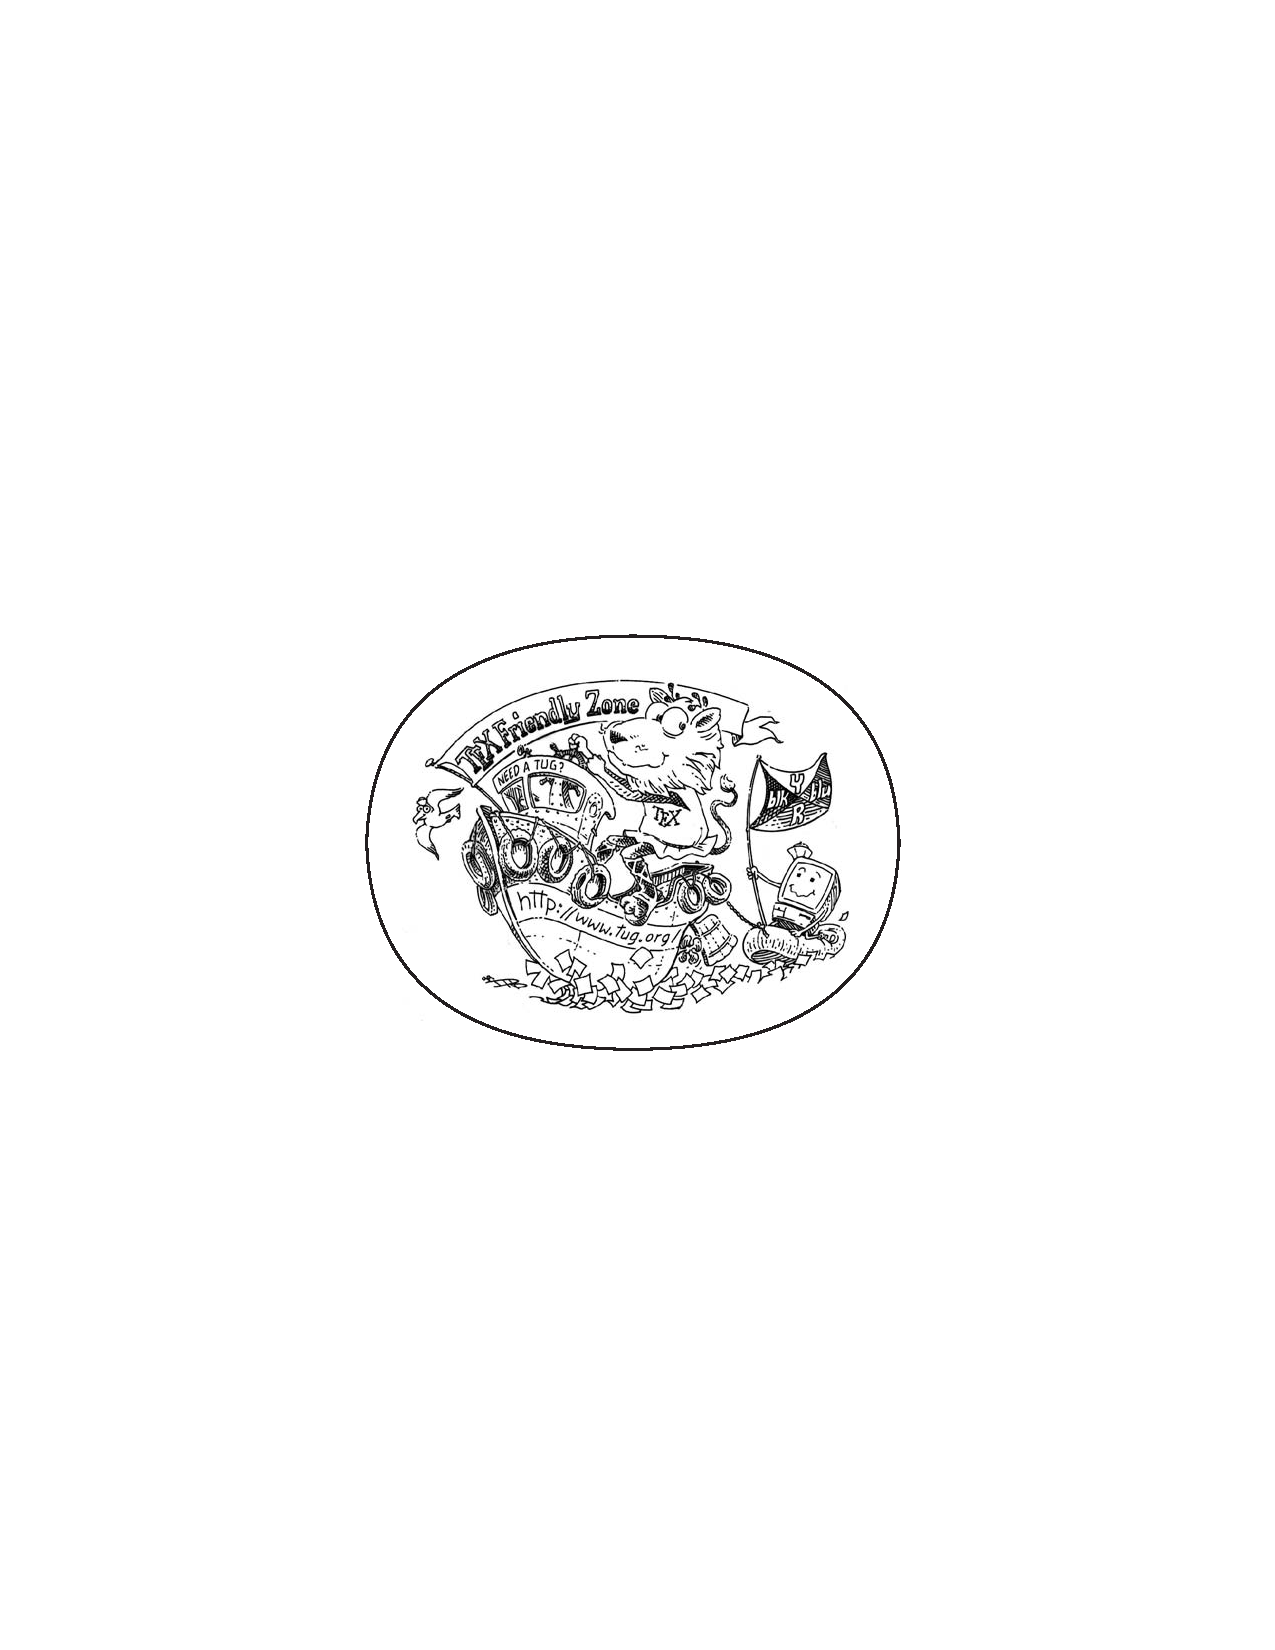
\includegraphics[width=6cm]{gfx/TFZsuperellipse_bw} \\ \medskip

        \mySubtitle \\ \medskip
        %\myDegree \\
        %\myDepartment \\
        %\myFaculty \\
        %\myUni \\ \bigskip

        \myTime\ -- \myVersion

        \vfill

    \end{center}
  \end{addmargin}
\end{titlepage}

\thispagestyle{empty}

\hfill

\vfill

\noindent\myName: \textit{\myTitle,} \mySubtitle, %\myDegree,
\textcopyright\ \myTime

%\bigskip
%
%\noindent\spacedlowsmallcaps{Supervisors}: \\
%\myProf \\
%\myOtherProf \\
%\mySupervisor
%
%\medskip
%
%\noindent\spacedlowsmallcaps{Location}: \\
%\myLocation
%
%\medskip
%
%\noindent\spacedlowsmallcaps{Time Frame}: \\
%\myTime

\cleardoublepage%*******************************************************
% Dedication
%*******************************************************
\thispagestyle{empty}
\phantomsection
\pdfbookmark[1]{Dedication}{Dedication}

\vspace*{3cm}

\begin{center}
    For Claudia and Emil \\ \smallskip
\end{center}

\cleardoublepage%*******************************************************
% Abstract
%*******************************************************
%\renewcommand{\abstractname}{Abstract}
\pdfbookmark[1]{Abstract}{Abstract}
% \addcontentsline{toc}{chapter}{\tocEntry{Abstract}}
\begingroup
\let\clearpage\relax
\let\cleardoublepage\relax
\let\cleardoublepage\relax

\chapter*{Abstract}
Everyday uses of audio recordings involve mixture signals: music contains a mixture of instruments; in a meeting or conference, there is a mixture of human voices.
Although human listeners find it easy to focus their attention on a particular sound source, automatically counting and separating sources remains a challenging task.
When two instruments play the same note (unison) or when many people speak concurrently (``cocktail party''), the overlap is severe, highlighting the need for new representations and powerful models to address these two tasks.
A common assumption when separating sources in the time-frequency domain (as in the case of non-negative matrix factorization) is that they are not fully overlapped.
Accurately estimating the number of sources is very important for real-world scenarios.
However, most approaches have relied on non-overlapping segments to facilitate ``counting by detection'' but with a higher amount of overlap, strategies need to shift towards directly inferring a count.
To address both problems, we used conventional signal processing techniques as well as deep neural networks (DNN).
We first address the source separation problem for unison instrument mixtures, 
thoroughly studying the distinct spectro-temporal modulations caused by vibrato. 
To exploit these modulations, we develop a method based on time warping informed by an estimate of the fundamental frequency. 
For cases where such estimates are not available, we present an unsupervised model, inspired by the way humans group time-varying sources (common fate).
This contribution comes with a novel representation that increases separability for overlapped and modulated sources on unison mixtures but also improves vocal/accompaniment separation when used as an input for a DNN model.
We approach the count estimation task by studying how humans can solve this tasks by conducting listening experiments, confirming that humans are only able to estimate up to four sources correctly.
To answer the question if machines can perform similarly, we present a DNN architecture, trained to estimate the number of concurrent speakers in a cocktail party scenario of up to ten speakers.
Our results show improvements compared to other methods, and the model even outperformed humans on the same task.
In this thesis, we affirmed the importance of modulation based signal separation. 
Our speaker count estimation model enables applications such as crowd surveillance or speaker diarization in challenging environments.
Finally, we inspected our count estimation model to glean insights on how it achieves its high performance, finding that modulations also play a crucial role in its workings.

\vfill

\begin{otherlanguage}{ngerman}
\pdfbookmark[1]{Zusammenfassung}{Zusammenfassung}
\chapter*{Zusammenfassung}

In unserem Alltag sind wir ständig von Signalmischungen umgeben: Musik  besteht aus einer Mischung von Instrumenten; in einem Meeting oder auf einer Konferenz sind wir Mischungen der menschlichen Stimme ausgesetzt.
Obwohl es für den menschlichen Zuhörer leicht ist, seine Aufmerksamkeit auf eine bestimmte Klangquelle zu fokussieren, bleibt die automatische Zählung und Trennung der Quellen eine anspruchsvolle Aufgabe.
Wenn zwei Instrumente die gleiche Note spielen (Unisono) oder wenn viele Menschen gleichzeitig sprechen (``Cocktail-Party''), ist die Überlappung groß, was die Notwendigkeit an neuen Repräsentationen und leistungsfähiger Modelle zur Bewältigung dieser beiden Aufgaben unterstreicht.
Bei der Trennung von Quellen im Zeit-Frequenzbereich (wie bei der nicht-negativen Matrixfaktorisierung) wird häufig angenommen, dass die Quellen nicht vollständig überlappt sind.
Die meisten Ansätze haben sich jedoch auf nicht überlappende Segmente konzentriert um eine Zählung durch Erkennung zu erleichtern, aber mit einer grösseren Überlappung müssen die Strategien hinzu eine direkten  Anzahl verlagert werden.
Die genaue Schätzung der Anzahl von Quellen ist für reale Szenarien sehr wichtig.
Um beide Probleme zu lösen, verwendeten wir sowohl konventionelle Signalverarbeitungstechniken als auch tiefgehendes neuronale Netze (DNN).
Wir gehen zunächst auf das Problem der Quellentrennung für unisono Instrumentenmischungen ein und untersuchen gründlich die unterschiedlichen zeitlich-spektralen Modulationen, verursacht durch Vibrato. 
Um diese Modulationen auszunutzen, entwickeln wir eine Methode, die auf dem Zeitverzerrung basiert und eine Schätzung der Grundfrequenz als zusätzliche Information nutzt.
Für Fälle, in denen diese Schätzungen nicht verfügbar sind, stellen wir ein unüberwachtes Modell vor, das inspiriert ist von der Art und Weise  wie Menschen zeitveränderliche Quellen gruppieren (Common Fate).
Dieser Beitrag enthält eine neuartige Repräsentation, die die Separierbarkeit für überlappte und modulierte Quellen in  Unisono-Mischungen erhöht, aber auch die Trennung in Gesang und Begleitung verbessert, wenn sie eingangs für ein DNN-Modell verwendet wird.
Wir bearbeiten die Aufgabe, die Anzahl von Quellen zu schätzen, indem wir zunächst untersuchen wie Menschen diese Aufgaben durch Hörversuche lösen können und bestätigen, dass Menschen nur in der Lage sind, bis zu vier Quellen korrekt in der Anzahl zu schätzen.
Um die Frage zu beantworten, ob Maschinen diese Aufgabe ähnlich gut bewältigen können, stellen wir eine DNN-Architektur vor, die erlernt hat, die Anzahl der gleichzeitigen Sprecher in einer Cocktail-Party-Umgebung von bis zu zehn Sprechern zu schätzen.
Unsere Ergebnisse zeigen Verbesserungen im Vergleich zu anderen Methoden, und das Modell übertraf sogar die Leistung des Menschen bei in der gleichen Aufgabe.
In dieser Arbeit haben wir bestätigt, wie wichtig die modulationsbasierte Signaltrennung ist. 
Unser Modell zur Schätzung der Sprecherzahl ermöglicht Anwendungen wie die Überwachung von Menschenmassen oder die beantwortung der Frage nach ``Wer spricht wann?'' in schwierigen Umgebungen.
Schließlich haben wir unser Schätzmodell für die Anzahl genau untersucht, um Erkenntnisse darüber zu gewinnen, warum es so leistungsfähig ist, und festgestellt, dass Modulationen auch hier eine entscheidende Rolle spielen.
\end{otherlanguage}

\endgroup

\vfill

\cleardoublepage%*******************************************************
% Publications
%*******************************************************
\pdfbookmark[1]{Publications}{publications}
\chapter*{Publications}
Chapters 4-8 of this thesis is mainly build upon the following publications that I published as first author during my time as a doctoral student.

\newcommand*{\boldnames}{}

\newbibmacro*{name:bold}[2]{%
  \def\do##1{\ifstrequal{#1, #2}{##1}{\bfseries\listbreak}{}}%
  \dolistloop{\boldnames}}


\xpretobibmacro{name:last}{\begingroup\usebibmacro{name:bold}{#1}{#2}}{}{}
\xpretobibmacro{name:first-last}{\begingroup\usebibmacro{name:bold}{#1}{#2}}{}{}
\xpretobibmacro{name:last-first}{\begingroup\usebibmacro{name:bold}{#1}{#2}}{}{}
\xpretobibmacro{name:delim}{\begingroup\normalfont}{}{}
\xapptobibmacro{name:last}{\endgroup}{}{}
\xapptobibmacro{name:first-last}{\endgroup}{}{}
\xapptobibmacro{name:last-first}{\endgroup}{}{}
\xapptobibmacro{name:delim}{\endgroup}{}{}

% \DeclareNameAlias{default}{last-first/first-last}

\DeclareFieldFormat{labelnumberwidth}{#1\adddot}
\newlength{\periodwidth}
\settowidth{\periodwidth}{.}

\defbibenvironment{numbered+bold}
  {\list
     {\printtext[labelnumberwidth]{%
        \printfield{prefixnumber}%
        \printfield{labelnumber}%
        }%
     }%
  {
   \setlength{\labelwidth}{\labelnumberwidth}%
   \setlength{\leftmargin}{\labelwidth}%
   \setlength{\labelsep}{\biblabelsep}%
   \addtolength{\labelsep}{1em}
   \addtolength{\leftmargin}{\labelsep}%
   \setlength{\itemsep}{\bibitemsep}%
   \setlength{\parsep}{\bibparsep}}%
   \renewcommand*{\makelabel}[1]{\hss##1}%
  }
  {\endlist}
  {\item\hskip-\periodwidth}


\newrefcontext[sorting=ynt]
\section*{Main Publications}

\begin{itemize}
  \item[\cite{stoeter19}] ~\fullcite{stoeter19}.
  \item[\cite{stoeter18}] ~\fullcite{stoeter18}.
\end{itemize}
\noindent
The publications were a result of collaboration with Soumitro Chakrabarty and Emanuël Habets. 
My contribution to this work was the initial problem formulation and the core idea to address the problem using deep neural networks. Furthermore, I designed the dataset design experimental design, and evaluation.
My college Soumitro Chakrabarty contributed to the development of the deep learning method; Emanuël Habets and Bernd Edler revised the articles.

\begin{itemize}
  \item[\cite{stoeter16}] ~\fullcite{stoeter16}.
\end{itemize}
\noindent
My contribution to this work was the experimental design, implementation and evaluation.
The original idea was developed by Antoine Liutkus, who also helped formulating the theory. Paul Magron provided code and results to compare with the HR-NMF method. Roland Badeau and Bernd Edler revised the article.

\begin{itemize}
  \item[\cite{stoeter15icassp}] ~\fullcite{stoeter15icassp}.
\end{itemize}
\noindent
My contribution in this work was the initial idea, literature overview of $F0$ estimation algorithm and the evaluation of the algorithms.
The work was done in close collaboration with my colleague Nils Werner who contributed to the efficient implementation of the $F0$ warping algorithm and the generation of appropriate warp contours to match mathematical constraints of time-warping. Bernd Edler revised this thesis.

\begin{itemize}
  \item[\cite{stoeter15acm}] ~\fullcite{stoeter15acm}.
\end{itemize}
\noindent
My contribution in this work was the initial idea which was inspired by the gap in existing $F0$ estimation datasets not providing sufficient level of annotation to derive an accurate ground truth.
The work was done together with our student, Michael Müller, who greatly helped to design and manufacture the custom experiment hardware, organize the actual recording and provide an assistance in analyzing and converting the recorded data.

\begin{itemize}
  \item[\cite{stoeter14}] ~\fullcite{stoeter14}.
\end{itemize}
\noindent
My contribution to this work was the initial idea, as well as the experimental design, and evaluation.
My college Stefan Bayer contributed important insights about the theory and implementation of time warping framework and formulated the mathematical notation therein. Bernd Edler revised the article.

\begin{itemize}
  \item[\cite{stoeter13}] ~\fullcite{stoeter13}.
\end{itemize}
\noindent
The work was based on a collaboration with Michael Schöffler and Jürgen Herre.
My contribution to this work was the initial idea, as well as the experimental prototype design, and evaluation.
My college Michael Schöffler contributed to the development of the web based evaluation software that later led to a follow-up publication~\cite{schoeffler13} which I co-authored. The article was revised by Jürgen Herre and Bernd Edler.



\section*{Additional Publications}
The following publications were not reprinted in this thesis but are nonetheless very closely related to audio based methods presented in this thesis.
\begin{refsection}[ownsideref.bib]
\nocite{*}
\printbibliography[env=numbered+bold, heading=none,resetnumbers=true, sorting=ynt]
\newrefcontext[sorting=nyt]
\end{refsection}

\section*{Open Datasets and Software}
To foster reproducible research, the following datasets and code were contributed under open licenses:
\begin{refsection}[owndata.bib]
\nocite{*}
\printbibliography[env=numbered+bold, heading=none,resetnumbers=true, sorting=ynt]
\newrefcontext[sorting=nyt]
\end{refsection}

\cleardoublepage%*******************************************************
% Acknowledgments
%*******************************************************
\pdfbookmark[1]{Acknowledgments}{acknowledgments}

\bigskip

\begingroup
\let\clearpage\relax
\let\cleardoublepage\relax
\let\cleardoublepage\relax
\chapter*{Acknowledgments}

First of all, I want to thank my supervisor Prof. Dr.-Ing. Bernd Edler for all his help and support throughout all the years. Bernd is the nicest and kindest supervisor anyone could have: his door was always open for me to have fruitful discussions and solve tricky problems together and at the same time he was giving me enough freedom to allow me to develop my own research ideas.

\bigskip

Besides my advisor, I want to thank Prof. Gaël Richard for taking the time to review my thesis.

\bigskip
I also want to thank Dr. Antoine Liutkus for inviting me to Nancy for a summer research visit that resulted in so many good ideas and a great friendship!

\bigskip

I want to thank all the amazing people in the AudioLabs, which made my work in Erlangen so enjoyable: First, I want to thank Elke, Tracy and Day-See for all the administrative help and beyond. Then, I want to thank Stefan Turowski for his great technical management in the AudioLabs. Next, I want to thank all of the colleagues at the AudioLabs (in alphabetical order): 
Alexander Adami, Stefan Bayer, Stefan Balke, Sebastian Braun, Tom Bäckström, Soumitro Chakrabarty, Youssef El Baba, Alexandra Craciun, Christian Dittmar, Sascha Disch, Jonathan Driedger, Esther Feichtner, Johannes Fischer, Yesenia Lacouture Parodi, Emanuël Habets, Jürgen Herre, Nanzhu Jiang, Patricio Lopez-Serrano, Wolfgang Mack, Goran Markovic, Vlora Arifi Müller, Meinard Müller, Thomas Prätzlich, Sebastian Rosenzweig, Konstantin Schmidt, Michael Schöffler, Armin Taghipour, Stefan Turowski, Maja Taseska, Maria Luis Valero, Elke Weiland, Christof Weiß, Nils Werner, Frank Zalkow and Julia Zalkow. Thanks to the people at Fraunhofer IIS, especially to Sascha Disch, Christopher Oates, Frederik Nagel, Christian Uhle.
And I also want to thank Thomas Zeiser from the RRZE high performance cluster for his great support.
In this vein, I want thank to all the great scientific open source tools out there that powered most of the experiments in this thesis.
\bigskip

A big thank to the students and interns I supervised and I thank them for all the great work: Berkan Ercan, Erik Johnson, Aravindh Krishnamoorty, Jeremy Hunt, Bufei Liu and Qiao Wang. 
To Karlheinz Busch from the Bamberg Symphonic Orchestra, Johannes Huber and Michael Müller for making our datasets possible. 

\bigskip

To Annika, Lisa, Florian, Chris and Chris for the great time Nuremberg and to Mathieu, Cheryl and Elias for the warm welcome in Montpellier.
I also want to thank the Faller family for their great support during the hard times of writing this thesis.

\bigskip

I deeply thank my family --- Dagmar, Heinrich and Marion --- for supporting me in every point of time in my life.

\bigskip

And last but not least, I want to thank my beloved partner and friend Claudia who gave me so much joy and hope that this journey succeeds.

\bigskip

...and to my son Emil for his beautiful smile.

\endgroup

\cleardoublepage%*******************************************************
% Table of Contents
%*******************************************************
\pagestyle{scrheadings}
%\phantomsection
\pdfbookmark[1]{\contentsname}{tableofcontents}
\setcounter{tocdepth}{1} % <-- 1 includes up to sections in the ToC
\setcounter{secnumdepth}{2} % <-- 2 numbers up to subsections
\manualmark
\markboth{\spacedlowsmallcaps{\contentsname}}{\spacedlowsmallcaps{\contentsname}}
\tableofcontents
\automark[section]{chapter}
\renewcommand{\chaptermark}[1]{\markboth{\spacedlowsmallcaps{#1}}{\spacedlowsmallcaps{#1}}}
\renewcommand{\sectionmark}[1]{\markright{\textsc{\thesection}\enspace\spacedlowsmallcaps{#1}}}
%*******************************************************
% List of Figures and of the Tables
%*******************************************************
\clearpage
% \pagestyle{empty} % Uncomment this line if your lists should not have any headlines with section name and page number
\begingroup
    \let\clearpage\relax
    \let\cleardoublepage\relax
    %*******************************************************
    % List of Figures
    %*******************************************************
    %\phantomsection
    %\addcontentsline{toc}{chapter}{\listfigurename}
    % \pdfbookmark[1]{\listfigurename}{lof}
    % \listoffigures

    % \vspace{8ex}

    %*******************************************************
    % List of Tables
    %*******************************************************
    %\phantomsection
    %\addcontentsline{toc}{chapter}{\listtablename}
    % \pdfbookmark[1]{\listtablename}{lot}
    % \listoftables

    % \vspace{8ex}
    % \newpage

    %*******************************************************
    % List of Listings
    %*******************************************************
    %\phantomsection
    %\addcontentsline{toc}{chapter}{\lstlistlistingname}
    % \pdfbookmark[1]{\lstlistlistingname}{lol}
    % \lstlistoflistings

    % \vspace{8ex}

    %*******************************************************
    % Acronyms
    %*******************************************************
    %\phantomsection
    \pdfbookmark[1]{Acronyms}{acronyms}
    \markboth{\spacedlowsmallcaps{Acronyms}}{\spacedlowsmallcaps{Acronyms}}
    \chapter*{Acronyms}
    \begin{acronym}[UMLX]
        \acro{DRY}{Don't Repeat Yourself}
        \acro{API}{Application Programming Interface}
        \acro{UML}{Unified Modeling Language}
    \end{acronym}

\endgroup

%********************************************************************
% Mainmatter
%*******************************************************
\cleardoublepage
\pagestyle{scrheadings}
\pagenumbering{arabic}
%\setcounter{page}{90}
% use \cleardoublepage here to avoid problems with pdfbookmark
\cleardoublepage
% \include{Chapters/DAFx14_StoeterEdler}
\cleardoublepage
\ctparttext{You can put some informational part preamble text here.
Illo principalmente su nos. Non message \emph{occidental} angloromanic
da. Debitas effortio simplbificate sia se, auxiliar summarios da que,
se avantiate publicationes via. Pan in terra summarios, capital
interlingua se que. Al via multo esser specimen, campo responder que
da. Le usate medical addresses pro, europa origine sanctificate nos se.}

% %************************************************
\chapter{Introduction}\label{ch:introduction}
%************************************************

It is very likely that you know the following situation: you were at a crowded party and the next day your best friend, who was unable to join, asked you ``How many people where there?''. 
You then struggled to find an answer because you had such intense conversations with the guests that you were unable to put your focus on the other guests.
It turns out that this scene includes many interesting aspects that are relevant for this thesis.
\par
First, it reminds us that in our daily life, we are exposed to situations where multiple events overlap in time.
In the proposed example of the conversation at a party, it is obvious that our field of view is limited and we can not see the other guests in a crowd.
In contrast to our vision, we physically might have been able to listen to all sounds, but we deliberatively chose to focus on only few sources and attenuate others.
We know that humans are notably good at performing such a task.
In such a noisy environment we are able to steer our attention to one sound source, even without eye contact and using only a single ear~\cite{bregman90}.
However, this attention mechanisms prevents us from fully observing the acoustic scene.
\par
In the audio research community, the attenuation of undesired speakers, when multiple concurrent speakers are present, is actually known as the ``cocktail party problem''~\cite{haykin05}.
Since almost 70 years (~\cite{cherry53}), research is fascinated by the idea to create a machine that separate the sources in a mixture.
This problem is called \emph{source separation}.
Although most scientific efforts have focused on separation, our example highlights that just the number of sources is already an important information.
In fact, many separation methods rely on this information for the effectiveness of subsequent processing.
These two tasks, separating and estimating the number of sources, is not just limited to conversations also applies to music as well.
If we imagine to attend a music concert of our favorite band, it is likely that we focus on the lead vocalist and miss out many details of the background band.
Furthermore, both scenarios of music and speech mixtures have more in common: it is valid to assume that estimating the number of sources and separating them is easier when there is less \emph{overlap} of the signals.
% why?
And both tasks become even more challenging when sources are almost fully overlapped such as when multiple instruments playing the same exact same note (in unison).
In this unique scenario where sources are overlapped in time and frequency, observable differences between sources are difficult to obtain.
Here, it is important to note that sounds are not stationary but they vary with time.
In fact, instruments and our voice can have distinct modulations such as vibrato, created by a conscious physical manipulation of the sound, to make a sound more pleasant to the listener~\cite{fletcher01}.
\par
In this thesis, we want to investigate if modulations can be used to separate highly overlapped speech and music source signals and 
To address this question I want to to investigate scenarios where sources are highly overlapped.
We then want to study and develop representations that allow to improve analysis and processing of these signals.
Also we want to develop new methods to address source separation scenarios. 
These methods would be designed for the constrained scenarios where modulation effects can easily be exploited.
Also we want to transfer the results and insights gained by these controlled studies onto more real-world scenarios.
And last but not least to investigate and develop new methods to address the task of estimating the number of sources in highly overlapped mixtures.

TODO: check if scope is clear (not promise too much)

% [X] Tell a story, and tell it well
% [X] Tell the reader the problem you are tackling in this project.
% [ ] Quote data sources, e.g., industry analysts, market surveys, case studies 
% [ ] Use plenty of concrete examples (or a running example) and figures 
% [X] State clearly how you aim to deal with this problem.
% [ ] Limit the scope of your study.

\clearpage
\section{Summary of Contributions}

This thesis comes with five main contributions:

\begin{enumerate}
\item I discuss scenarios of time and frequency overlapped audio sources.
I consider known scenarios for speech and music but also present a novel scenario where instruments are playing in unison.
In this scenario, I show, how slowly varying tempo-spectral modulations, caused e.g. by vibrato, can be utilized for separation and source count estimation of highly overlapped signals.
Furthermore I show how these scenarios can stimulate new research directions to \emph{analyze} and \emph{process} such signals.\\

\item I developed two novel methods to \emph{separate} unison instrument mixtures: one is informed by an estimate of the fundamental frequency variation.
% TODO: we also improved F0 estimation
The other is unsupervised, inspired by the way how humans segregate time-varying sources.
Finally, I study how the observations from the unison scenario can be transferred to real world scenarios such as the separation of professional produced music.\\

\item I provide two detailed experimental studies to assess how humans perceive highly overlapped mixtures.
In these studies I focussed on the \emph{number of concurrent sources} in scenarios such as a overlapped speech as well as polyphonic music recordings.
In this vein, I present the results of auditory experiments that studied the humans ability to detect the maximum number of sources.\\

\item For the task of \emph{estimating the maximum number of concurrent} speakers I developed a method based on deep neural networks that addresses ``cocktail party'' like environments.
Furthermore, I show that this model reached state-of-the art performance when compared to other models and also supersedes human performance when compared with the results of subjective listening experiments.
Finally I revealed the relation between slow modulations in speech and the ability of a model to count.\\

\item I co-organized the international source separation evaluation campaign (SiSEC) and helped to improve sustainability and reproducibility in our field by providing service the research community. In that vein, I provided tools to assess the quality of separation system. These tools were also used throughout the work presented in this thesis.
\end{enumerate}

This thesis is based on the previously listed publications. As such, they are cited repeatedly throughout this thesis. For readability reasons, if a section is mainly based on one of these publication, a remark is added at side of the page, instead of citing the same publication exhaustively. Furthermore, it should be noted ––– if not stated otherwise ---  that these contributions in the publications are based on the ideas and research of the author of this thesis.

\section{Structure of this Thesis}

The thesis and its relevant linked publications are organized into 6 main chapters.
\begin{description}
  \item[Chapter 2] explains the fundamental concepts of audio signals (Section~\ref{sec:specifics-of-audio-signals}) as well as sources and overlapped sounds (Section~\ref{sources-and-mixtures}), relevant for the remainder of this thesis. 
  This includes commonly used transformations and signal representations for the task of source separation and source count estimation.
  Furthermore, the process of mixing sound sources as well as its inverse task --- sound source separation --- are explained.
  The chapter also covers basics of fundamental frequency and its variations (Section~\ref{sub:time-variant-audio-signals}) as an important feature for harmonic audio signals.
  Part of this chapter is based on~\cite{rafii18}.
  \item[Chapter 3] introduces relevant tasks and applications in the context of highly overlapped sounds.
  Furthermore, the relevance of highly overlapped source scenarios are discussed and the research track of slow  modulations (Section~\ref{exploiting-slow-modulations}) to address separation tasks is proposed.
  \item[Chapter 4] presents and discusses the importance of data for analysis and evaluation.
  In this chapter synthetic (Section~\ref{}) and realistic (Section~\ref{}) datasets are presented, created during the course of this thesis~\cite{oss_wice, oss_unison, oss_libricount, stoeter15acm, liutkus17}.
  \item[Chapter 5 and 6] presents separation methods that are developed over the course of this thesis. 
  The covers techniques that utilize modulation information when available(Chapter 5, ~\cite{stoeter14, stoeter15icassp}) as well as blind methods (Chapter 6~\cite{stoeter16, liutkus17}).
  \item[Chapter 7 and 8] covers the analysis of overlapped sounds. Specifically, it deals with identifying and estimating the number of sources on music~\cite{schoeffler13, stoeter13} and the cocktail party scenario~\cite{stoeter19, stoeter18}.
  \item[Chapter 9] Concludes this thesis and gives a and outlook into future research directions.
\end{description}

% \hypertarget{Fundamentals of Overlapped Sounds}{%
\chapter{Fundamentals of Overlapped Sounds}\label{cha:fundamentals}}

In this thesis, the core part is focussed on \emph{analysis} and \emph{processing} of sound recordings of music and speech, commonly referred to as \emph{audio signals}.
In this chapter, we introduce basic concepts of digital audio signals which are relevant to apprehend the remaining chapters.

\hypertarget{Audio Signals}{%
\section{Audio Signals}\label{sec:specifics-of-audio-signals}}

When a sound wave travels through a medium like air, a signal can be captured using a microphone by measuring the local pressure deviation over time.
Such a signal can be written as a function \(x(t)\), continuous in both time \(t \in \sR\) and the amplitude \(x(t) \in \sR\).
An \emph{audio signal} is meant to be perceived by the human auditory system --- through our ears.
Therefore, we can observe specific properties, consistent with the limitations of the human hearing, for example in dynamics as well as in limited signal bandwidth.
Many other signals exist with similar characteristics such as signals from finance, geophysics, meteorology or medical data.
The result is that audio research is inspired by applications of other fields of signal processing and vice versa.

\hypertarget{digital-representations-of-audio-signals}{%
\subsection{Digital Representations of Audio
Signals}\label{digital-representations-of-audio-signals}}

Today, digital representations are used to store, analyze or process audio signals conveniently.
A digital audio signal can be obtained from an analog signal using analog-to-digital/digital-to-analog converters (ADC/DAC) which can be found in almost any every-day device such as laptops and smartphones.
In short, this process includes two steps: first, the continuous time signal \(x(t)\) is converted to a discrete time series, so that one sample\footnote{Please note, that the use of the word \emph{sample} will have different meanings in the context of machine learning, where a sample is an instance of a full signal instead of a single time step.} \(x_n\) was \emph{sampled} with equidistant steps \(T\); second, the amplitude values can be \emph{quantized}, resulting in a vector \(\vx \in \sZ\), represented as a one dimensional time series of amplitudes.
An important parameter in the process of digitization is the sample rate \(F_s = 1/T\) where \(T\) is the sampling period.
% Often, \(F_s\) has a significant effect on the quality of audio signals.
% And, it is the objective of a real-world audio system not to introduce perceivable degradation in audio quality when a digital signal is reproduced over headphones or loudspeakers.
% Due to the Nyquist-Shannon sampling theorem, the sample rate needs to be at least twice the bandwidth of the analog signal.
To facilitate the full human hearing range of 20~\si{\hertz} - 20~\si{\kilo\hertz}~\cite{fastl90, moore89}, due to the Nyquist-Shannon sampling theorem, often, sample rates of at least 40~\si{\kilo\hertz} are chosen.
However, for many applications, a lower sampling rate is sufficient, e.g., in speech communication where intelligibility often is more important than quality.
For further details, we refer the reader to audio signal processing basics such as~Chapter 1 in~\cite{proakis96} or Chapter 2 in~\cite{Mueller15}.

\hypertarget{time-frequency-representation}{%
\subsection{Time-Frequency Representation}\label{sub:time-frequency-representation}}

We often analyze sounds in the frequency domain where the reduced redundancy of the signal improves the computational efficiency of signal processing methods, especially for speech and music that have periodicities.
It is common to achieve this through the use of discrete Fourier transform (DFT) and its fast FFT implementation~\cite{cooley65} (for details, the reader is referred to~Chapter 4 of~\cite{proakis96}).
Spectral representations also relate to our human auditory system~\cite{zwicker13, moore89}, allowing us to process sounds closer to how we perceive them.
\par
The periodicity of real-world sounds, usually only holds for short durations of several milliseconds, often referred to as \emph{quasi-stationarity}.
We analyze and process short-time spectra, computed in an overlapped fashion, resulting in a \emph{time-frequency} (TF) representation.
The short-time Fourier transform (STFT) is the most commonly used TF representation~\cite{mcaulay86}.
It encodes the time-varying spectra into a matrix \(\mX\) with frequencies \(k\) and time frames \(n\).
\par
STFT matrices \(\mX \in \sC^{n \times k}\) are complex and include phase information.
When sounds are processed in the time-frequency domain, the transformation greatly benefits from being invertible to reconstruct a time domain signal.
However, analysis and processing is often focussed  on the \emph{magnitude} \(|\mX|\) or the \emph{spectrogram} \(|\mX|^2\).

\subsection{Fundamental Frequency and Harmonicity}

\begin{figure}[h!]
  \centering
  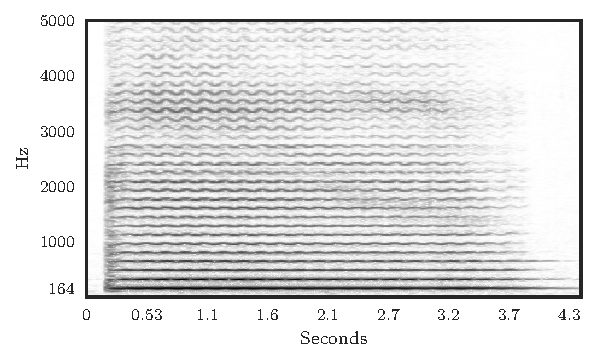
\includegraphics[width=0.8\columnwidth]{gfx/cello.pdf}
  \caption{Spectrogram of single violoncello note (E3) of a fundamental frequency \(F_0\) of about 164\si{\hertz}. The vibrato is clearly visible in the upper part of the harmonic spectrum. X-axis shows time (in seconds), y-axis depicts frequency (in Hertz). The audio signal is part of the MUSERC dataset~\cite{stoeter15acm}.}%
  \label{fig:cello_example}%
\end{figure}

Speech and music signals are characterized by its periodicity.
And it is this property we perceive as \emph{pitched}.
\emph{Pitch} is defined by Klapuri in~\cite{klapuri06book} as 

\begin{quote}
``a perceptual attribute which allows the ordering of sounds on a frequency-related scale extending from low to high.''
\end{quote}

It is important to note that \emph{pitch} is a subjective measure.
The objective equivalent is referred to as the \emph{fundamental frequency} (\(F_0\))\footnote{Pitch and $F_0$ are often used synonymously in audio research. 
Even though this is incorrect, we sometimes may refer to other work where pitch instead of $F_0$ is used.}.
All frequencies together formed by the integer multiples of the fundamental frequency are named \textit{harmonics}~\cite{schenker54}.
\(F_0\) can be defined as the lowest frequency/partial of a harmonic signal.
An example of a harmonic signal can be seen in Figure~\ref{fig:cello_example} that depicts a single note (E3) played by violoncello.
When the fundamental frequency changes, the frequencies of these harmonics change accordingly.
This results in the typical comb-like structure of harmonic signals when analyzed in the time-frequency domain.
For a detailed overview into the research field of pitch and \(F_0\), the reader is referred to~\cite{klapuri06book}.

\subsection{Time-Variant Audio Signals}\label{sub:time-variant-audio-signals}

Audio signals are considered to be stationary or time-invariant when their properties such as the amplitude of the fundamental frequency of the signal do not change over time.
% A stationary sound can turn into time-invariant sound using modulations
The signal becomes time-variant when an external function changes (modulates) the parameters of a signal over time.
This type of modulation was the basis for many break-through inventions such as radio transmission~\cite{shannon48}.
In the case of audio signals, often both the modulating function (modulator or carrier) and the signal being modulated (input), are periodic.
Signal modulations are often created intentionally but also occur naturally in many real-world audio signals such as speech.
In the following, we will present audio modulation categories and their cause, underlining the importance of them.

\subsubsection*{Audio Signal Communication}

Audio modulations play an essential role in the transmission of audio signals such as in radio broadcasting.
It is based on the principle of a modulator/demodulator (modem) where a high-frequency carrier signal is modulated by a (lower frequency) audio signal to be transmitted.
The modulator varies the amplitude or the frequency of the carrier signal.
Let us imagine a sinusoidal carrier signal $x(t) = \sin \omega_c t$ where $\omega_c$ is the carrier frequency. Now, applying a time varying amplitude $a(t)$ results in \emph{amplitude modulation} (AM):

% We assume that we can separate overlapping partials of the sources based on differences in amplitude and/or frequency modulation, resulting in the following model for a signal with $P$ commonly modulated partials
% \begin{equation}
%   \begin{array}{l}
%    x(n) = \displaystyle \sum_{p=1}^{P} \Big[\big(1 + a(n)\big) \\
%    \hspace{3.5em}\displaystyle \cdot\sin \Big(2\pwe f_{p,0}\big(n + \frac{1}{f_{1,0}} \sum_{m=m_0}^{n}{f(m)} \big) + \phi_{p,0} \Big)\Big] ,
%   \end{array}
% \end{equation}
% where effectively the amplitude modulation is $a(n)$ and the frequency modulation of the first partial is $f(n)$.

\begin{equation*}
    s_{AM}(t) = a(t) \sin \left( \omega_{c} t\right).    
\end{equation*}

In comparison to AM, frequency modulation (FM) varies the frequency of the carrier, so that:

\begin{equation*}
    s_{FM}(t) = A \sin \left( \omega_{c} t + p_0 + M_f \int f(t) dt \right)
\end{equation*}

where A is the amplitude, $\omega_{c}$ is the carrier frequency and $M_f$ is called modulation index.
When the modulation function $f(t)$ is a single sine wave, $\cos \left(\omega_{m} t+p_{m}\right)$, of frequency $\omega_{m}$, the Fourier spectrum of $s_{FM}(t)$, in theory, depends on Bessel functions that do not admit a closed-form expression, being intractable in practice~\cite{abramowitz64}.
% For applications where the modulation frequencies are a lot smaller than the carrier frequency, the spectrum that results by frequency modulations is similar to those of amplitude modulations.
% This is the reason why algorithms that aim to capture the amplitude modulation will also observe frequency modulations.
% The total bandwidth in this scenario is approximately $2\Delta \omega_0$, as found by Carson in~\cite{carson22}.\par
For audio communication such as FM radio, the modulation frequency or rate is the same as the audio signal being transmitted (audio rate modulations).
In music signals, the carrier could be a single note, played by a violin and the modulation signal is the movement of the finger on the fretboard, producing a vibrato effect.
In music or speech, these modulations are much slower --- typically up to 10~\si{\hertz} (slow) or up to 100~\si{\hertz} (medium/fast).

\subsubsection*{Modulations in Music --- Vibrato}

Both, frequency and amplitude modulations are a recurrent phenomenon in music as well.
In traditional instruments, modulations are known to as \emph{vibrato}, defined by~\cite{seashore31} as

\begin{quote}
``...a periodic pulsation, generally involving pitch, intensity, and timbre, which produces a pleasing flexibility, mellowness and richness of tone.''
\end{quote}

Pitch and intensity vibrato can directly be mapped to AM and FM, a timbre vibrato, however, is not easily defined and describes a joint AM/FM modulation~\cite{desain99}.
Vibrato is an essential playing style for string instruments like a violin. 
For these instruments, that are usually plucked or bowed, the strings are the primary source of excitation that is modulated in frequency by the player's finger on a fretboard~\cite{macleod06}.
Modulations are also present in woodwind and brass instruments; however, instead of the excitation signal, the modulations affect the resonator.
Many musicians use similar modulation rates to perform a vibrato, usually in the range of 4-8\si{\hertz}.
A detailed overview of the different musical instruments and their modulation characteristics is presented in~\cite{fletcher01}.
\par
Real instruments are not capable of purely amplitude modulated sounds (\emph{tremolo}). 
Today, however, many instruments are electric or attached to electronic effects where pure modulations can be applied using digital or analog signal processing.
For example, popular electric pianos like the ``Fender Rhodes'' can include an optional tremolo effect\footnote{Even though it is labeled as \emph{vibrato}.}.
In its most pure form, synthesizers like~\cite{pinch09, buchla05} allow modulating almost any parameters of a sound using low-frequency oscillators (LFOs) or envelopes that produce sinusoidal, square or triangle functions of any rate.
One of the most important sound synthesis methods --- FM Synthesis --- became popular in the early days of digital signal processing. 
Chowning found in~\cite{chowning73} that the modulation of sinusoids using audio rate modulators provides a computationally efficient way of producing fairly complex sounds which mimic, e.g. piano sounds using just four sinusoidal modulators.
\par
It turns out that instrumental vibrato has similar properties compared to vibrato produced in singing voice.
Vocal vibrato mainly depends on frequency modulation even though amplitude fluctuations are present~\cite{sundberg94}. 
Vocal vibrato rates are similar to that of instrumental vibrato rates with an average of 5~\si{\hertz}.
However, analysis of exceptional voices such as from Freddie Mercury~\cite{herbst17}, shows peak rates of up to 7~\si{\hertz}.

\subsubsection*{Modulations in Speech}

Unlike singing voice, speech modulations are part of human communication and therefore part of our language.
Modulations in speech include medium to fast modulations of up to a few hundred Hertz, perceived as \emph{roughness} or \emph{residue pitch}.
However, often research is focussed on slow modulations around 4~\si{\hertz}~\cite{greenberg97, fuellgrabe09} that correlate to the syllable rate~\cite{plomp83, houtgast85}.
In fact, it was found in~\cite{joris04} that speech is the reason why our human auditory system is so sensitive to amplitude modulations and even our brain is capable of processing rhythm-like envelope fluctuations of the same rate~\cite{schreiner88, plomp83}.

\subsubsection*{The importance of Slow Modulations}

% Table~\ref{tab:modulations} summarized the many types of modulations in audio signals.
It is interesting to observe that many modulations have a rate of around 5~\si{\hertz}. 
Zwicker found in~\cite{zwicker52} that humans are very sensitive at detecting amplitude modulations at such a low modulation frequency.
This observation can be confirmed when looking at physical modulations that occur when humans suffer from vocal tremor~\cite{ramig87} or Parkinson~\cite{botzel14}: in both cases, muscle contractions are actuated with the same frequency, indicating that these modulations are natural for humans.

% \begin{table}[]
% \scriptsize
% \centering
% \begin{adjustbox}{angle=90}
% \begin{tabular}{@{}lllp{3.5cm}ll@{}}
% \toprule
%                           & Carrier Signal    & Modulation Function & Modulated Parameters        & Modulation rate & References\\ 
% \midrule
% AM/FM/PM                  & HF Sinusoid       & any audio signal    & amplitude, frequency, phase & up to 20~\si{\kilo\hertz}     & \cite{shannon48}        \\
% String Vibrato & String Excitation & sinusoidal-like     & string length   & 5-7~\si{\hertz}          & \cite{fletcher01, macleod06}\\
% Woodwind and Brass Vibrato & Resonator & sinusoidal-like & amplitude, timbre               & 4-8~\si{\hertz}          & \cite{fletcher01, gilbert05}\\
% Modular Synthesizer       & any audio signal  & LFO                 & any parameter               & not limited     & \cite{buchla05, pinch09}\\ 
% Electronic Organ with Tremolo  & instrument sound & doppler effect      & amplitude and frequency & 1~\si{\hertz}/7~\si{\hertz} & \cite{leslie49} \\
% Singing Voice  & vocal &  sinusoidal/triangular &  amplitude and frequency & 5-8~\si{\hertz} & \cite{sundberg94} \\
% Speech  & glottal pulse, language & not defined & amplitude, frequency, \newline phoneme duration, timbre& 4-10~\si{\hertz} & \cite{plomp83, fuellgrabe09}\\
% Parkinsonian tremor  & muscle activity &  sinusoidal-like & amplitude & 5~\si{\hertz} & \cite{botzel14}\\
% Auditory cortex  & nerve activity &  sinusoidal-like & amplitude & up to 20~\si{\hertz} & \cite{schreiner88}\\
% \bottomrule
% \end{tabular}
% \end{adjustbox}
% \caption{Overview of modulations in audio signals and a selection of their respective properties.}%
% \label{tab:modulations}
% \end{table}

\hypertarget{sources-and-mixtures}{%
\section{Sources and Mixtures}\label{sources-and-mixtures}}

In the real world, single isolated audio signals are rare.
Instead, we are faced with sets of \emph{sound sources} that make up an \emph{acoustical sound scene}.
When multiple sources are active at the same time, the sound that reaches our ears or is recorded using a microphone is superimposed or \emph{mixed} to a single sound.
A \emph{mixture} represents a mapping from a set of sources \(\mathbf{s}\) to an output signal \(\mathbf{x}\).
There exist a variety of different mixing models that are utilized in literature.
\par
Usually, these are built upon several assumptions to constrain the scenario and model specific aspects of real-world signals.
The most important assumption is that the mixture is the linear sum of all sources.
Another differentiation is made between instantaneous or convolutive mixtures.
For instantaneous mixtures, all sources are mixed using fixed mixing parameters \(a_j\).
This is the typical scenario when sources are mixed using a mixing console.
In \emph{convolutive} mixtures, each source \(\mathbf{s_j}\) is convolved by a filter response \(r_j\) before summation.
\par
Usually, the mixing process is assumed to be time-invariant but for a variety of signals, such as live recordings with moving sources, it can also be time-variant.
The mathematical notations of different mixing models are summarized in Table~\ref{tab:mixing_models}.
\par
In the remainder of this thesis, we will only consider the linear (instantaneous) case of time-invariant mixing, but many of the methods could be transferred to other cases.

\begin{table}[]
    \centering
\begin{longtable}[]{lll}
\toprule
\begin{minipage}[b]{0.26\columnwidth}\raggedright
\strut
\end{minipage} & \begin{minipage}[b]{0.32\columnwidth}\raggedright
Instantaneous\strut
\end{minipage} & \begin{minipage}[b]{0.3\columnwidth}\raggedright
Convolutive\strut
\end{minipage}\tabularnewline
\midrule
\endhead
\begin{minipage}[t]{0.26\columnwidth}\raggedright
Time-Invariant\strut
\end{minipage} & \begin{minipage}[t]{0.32\columnwidth}\raggedright
\(\mathbf{x}=\sum_{j=1}^{J}a_j\mathbf{s}_j\)\strut
\end{minipage} & \begin{minipage}[t]{0.3\columnwidth}\raggedright
\(\mathbf{x} = \sum_{j=1}^{J}r_{j} \ast \mathbf{s}_j\)\strut
\end{minipage}\tabularnewline
\begin{minipage}[t]{0.26\columnwidth}\raggedright
Time-Variant\strut
\end{minipage} & \begin{minipage}[t]{0.32\columnwidth}\raggedright
\(\mathbf{x}=\sum_{j=1}^{J}a_j(n)\mathbf{s}_j\)\strut
\end{minipage} & \begin{minipage}[t]{0.3\columnwidth}\raggedright
\(\mathbf{x} = \sum_{j=1}^{J}r_{j}(n) \ast \mathbf{s}_j\)\strut
\end{minipage}\tabularnewline
\bottomrule
\end{longtable}
    \caption{Overview of linear mixing models for a mixture \(\mathbf{x}\), sources \(\mathbf{s}_j\) and a filter response \(r_j\).}
    \label{tab:mixing_models}
\end{table}

\subsubsection*{Specifics of Music Mixtures}
\label{par:specifics_of_music_mixtures}

In music, the process of mixing is an essential step in the process of music creation.
Mixing sources are a creative task that involves recording engineers and tonmeisters, and often the artists itself.
In today's digital mastering processes, professionally produced music consists of several intermediate mixing steps before the final mixture is produced:

\begin{description}
  \item[1) Microphone Recording:] in this step, the analog sources are captured and A/D converted. 
  Vocals and other acoustic instruments are recorded using one or multiple microphones.
  Electric instruments such as electric guitars, keyboards or synthesizers may be amplified and then directly digitized.
  \item[2) Raw Source Image:] the digital raw source signals are grouped and mixed into a \emph{source image} (also \emph{stem}).
  This grouping involves a creative process; hence it is usually done by a recording engineer.
  The source image is mixed to a specific number of output channels (e.g., stereo) even though the recording may have used less (e.g., vocals) or more than two microphones (e.g., drums).
  In this stage, a panning is added to position the source images spatially.
  \item[3) Mastered Source Image:] for each of the images, an additional mastering step is being applied.
  At this stage, effects such as artificial reverberation are added.
  \item[4) Raw Mix:] the linear sum of all source images are mixed.
  \item[5: Mastered Mix:] Optionally, further mastering is applied.
  Often, this step involves non-linear processing such as dynamic range compression.
\end{description}

This emphasizes that the definition of a source is subjective and depends on the application and its context. In this thesis, we mainly deal with tasks where we observe 4) and want to obtain 3) which is a common restriction made in tasks that are concerned with professionally produced music~\cite{sisec16}.

\hypertarget{processing-and-analysis-of-mixtures}{%
\section{Processing and Analysis of Mixtures}\label{sec:processing-and-analysis-of-mixtures}}

While in many ways, mixtures are not different to any other audio signal, two research questions stand out prominently:

\begin{itemize}
    \item Can we obtain \(\vs_j\) from \(\vx\)? 
    \item Can we find \(J\) from \(\vx\)?
\end{itemize}

These two questions are addressed in the scientific fields of \emph{sound source separation} and \emph{source count estimation}.

\subsection{Sound Source Separation}

One of the earliest work on audio source separation started in the mid 70s~\cite{miller73}.
Since then a large number of contributions were made in this field, both, targeted at speech and music separation.
Due to this large number of contributions, it is hardly feasible to give an extensive overview of all existing methods in the context, and the reader is referred to~\cite{vincent18, comon10, rafii}.
\par
Source separation methods have relevant applications for music and speech mixtures such as attenuation of hearing aids, karaoke or music creation due to isolated sample composition.
It also indirectly helps for related tasks such as upmixing/remixing, improved music transcription or automatic speech recognition (ASR). 
\par
In the following, we present three ways to group separation scenarios:

\subsubsection*{Underdetermined vs. Overdetermined Separation}
As mentioned in Section~\ref{sources-and-mixtures}, generating sound mixtures is closely related to the process of mixing taken place during recording (speech) or with the help of professional recording engineers (music).
One assumption that was not mentioned before, is the importance of the number of sensors or microphones used to create the mixture.
A source separation problem is \emph{over-determined} when the number of sources is smaller than the number of sensors; \emph{determined} when they are equal.
For these two cases, a large number of method exist and in a closed form solution is possible.
The reader is referred to~\cite{common10}, which gives a detailed overview of these methods.\\
Many real-world source separation problems, however, are \emph{under-determined} and up to date for a large number of scenarios, the problem of separating sources is still very challenging.
\par
In this thesis, we only focus on methods that perform separation on underdetermined mixtures.

\subsubsection*{Single Channel vs. Multichannel Separation}
Today music recordings are mostly produced for stereo output. 
In many music recordings certain assumptions can be made (and utilized) of how sources are balanced between the two stereo channels. 
E.g., often in popular music, a fixed panning for the vocals is correctly assumed.
\par
As a large number of recording nowadays is still stored as single channel, in this thesis we want to focus on this single channel separation.

\subsubsection*{Blind vs. Supervised Separation}
A blind source separation system does not require additional information about the source signals, the location or acoustical environment to perform separation~\cite{makino07}.
In practice, blind source separation is ill-posed and it is not generally possible to find a single solution.
This why many proposed methods rely on additional information such as the acoustic environment, the musical score or the fundamental frequency~\cite{liutkus13, ewert14}.

\subsection{Vocal Accompaniment Separation}
The separation of music into two parts, the foreground lead (mostly the vocals) and the background accompaniment (drums, bass, other), is one of the most relevant scenarios in music separation with a large number of applications such as mixing karaoke or acapella tracks.
Vocal Accompaniment separation has specific issues and assumptions when compared to other separation scenarios like speech.
Many music separation methods often rely on knowledge about the mixing process as made in Table~\ref{tab:mixing_models}.
While there exist many source separation methods that aim to extract the actual raw audio recording, often it is sufficient to extract the source images from the raw mixture.
In a live recording, this results in inverting the process of convolution as well.
Separation of convoluted mixtures is a very active field in source separation described in~\cite{pedersen07}.
In the context of music separation, however, this becomes less relevant as today's recording and studio mixing environment are mostly digital.
Here, the last step in creating music mixtures, as described earlier, is a linear mix.
While the source images can yield from a mixing process undergoing the various assumptions, for the case of a mixture of source images, we consider only linear mixing in this thesis.
For a more detailed description of this scenario and applications of source image extraction, see~\cite{sturmel12}.
\par
Another specific about music separation is that it is typically restricted to a well-defined set of musical sources.
Often these restrictions need to be made because not for all kind of music separation scenarios, datasets are available.
Thus, the most popular task is to extract the vocals and the background of the music.
An extensive overview of music separation methods can be found in~\cite{rafii18}.
Even though the overview is focused on vocal accompaniment separation, most approaches can be generalized to other sources.
\par
To evaluate separation systems for this scenario, the majority of publications used the Blind Source Evaluation (BSS Eval) toolbox~\cite{fevotte05,vincent06} that provides ``different and complementary metrics for evaluating separation that measure the amount of distortion, artifacts, and interference in the results''~\cite{rafii18}.

\subsection{Estimating the Number of Sources}%
\label{sub:count_problemstatement}

\begin{figure}[ht!]
  \centering
  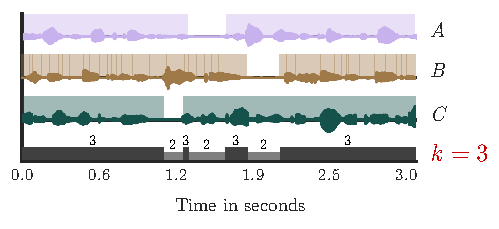
\includegraphics[width=0.8\columnwidth]{Chapters/08_Analysis_CountNet/figures/teaser.pdf}
  \caption{Illustration of three concurrent sources (A, B, C) and their respective activity. Bottom plot shows the mixture (input), the number of concurrently active sources and its maximum \(k\). Figure was published in ~\cite{stoeter18} \textsuperscript{\textregistered}2018 IEEE.}%
  \label{fig:teaser}%
\end{figure}

The number of sources is an important information to be used in source separation and many other related research fields.
In real-world applications, information about the actual number of concurrent speakers is often not available.
\par
The \emph{number of sources} \( \cardinality \in \mathbb{Z}^{+}_{0} \) appears to be a clearly defined property of a mixture. 
However, the meaning of it can differ, depending on its application.
Let us assume that we have \(L\) sources and a mixture of duration \(N\).
Further, we imagine a latent binary \textit{source activity} variable~$v_{nl}\in \left\{ 0,1 \right\}$ that indicates the activity of each source \(l\) and for each time instance \(n\).
Now, concerning the number of sources, two definitions of \(k\) can be imagined:

\begin{description}
\item[A)] maximum number of sources, even if not concurrently active. It is simply the sum of all sources that are active at least once within \(N\). This definition is more useful when the sources can be identified or detected first. This definition can also be considered as ``counting by detection''.
\item[B)] maximum number of concurrent sources even if the sources belong to the same class. Here, it represents the maximum of the mixtures concurrency. This definition is more useful as a preprocessing for a separation system since such a system would only require the number of auditory streams and not the number of (non-concurrent) sources. For such approaches it becomes possible to apply separation only when its ``needed''. This definition can also be considered as ``direct count estimation''\footnote{Note the subtle difference between ``counting'', which refers to a sequential process and ``count estimation'' or ``denumerating'', which directly relate to an integer.}.
\end{description}

At short time scales A) is equal to B) because the instrumentation usually does not change. 
In Fig.~\ref{fig:teaser}, we illustrate a setup featuring~$L=3$ unique sources.
At any given time, one can see --- given definition B) --- that at most~$k=L=3$ sources are active at the same time and~$k=2$ could be the outcome if a smaller excerpt would be evaluated.
In this thesis, we will pick definition B when concerned about developing methods to estimate the number of sources.
% \hypertarget{highly-overlapped-signals}{%
\chapter{Challenges of Highly Overlapped Signals}\label{cha:highly-overlapped-signals}}

In the previous chapter, I introduced signal processing in the context of audio mixtures. In this chapter, I focus on the challenges of highly overlapped signals.

\hypertarget{separability-of-mixtures}{%
\section{Separability of Mixtures}\label{separability-of-mixtures}}

Time-frequency representations such as the short-time Fourier transform (STFT) have clear benefits such as the improved interpretability due to its ``image-like'' two-dimensional properties.
More importantly, however, such a representation allows to separate mixtures of speech and musical instruments.
The reason for this is that these mixtures may be fully overlapped in the time domain but are less overlapped in the frequency domain~\cite{rickard02, giannoulis11, rafii}.
In turn, a time-frequency representation allows applying to filter in a way that sufficiently extracts all targets from the mixture.
Furthermore, it allows for the reconstruction of the original waveform and provides a good trade-off between computational complexity and separation quality.
\par
Due to these reasons, many source separation methods focus on extracting individual sources by modeling their respective target in the time-frequency domain.
Further, it is assumed that the STFT provides a sufficient level of separability.
The actual extraction or filtering is done by synthesizing the magnitude estimate of the model and applying the originals mixture phase.
\par
In practice, the ability to extract a source from a mixture depends on the amount of overlap between sources.
Without any overlap, separation is not necessary, and a small amount of overlap can be tolerated to extract the sources still sufficiently.
However, if sources are fully overlapped in both, time and frequency, a separation in the TF domain is hardly possible.
A metric that is often used for evaluation is called \emph{separability} and was found by Rickard in~\cite{rickard02} as a useful metric for both, speech and music~\cite{giannoulis11} signals.
\par
In linear mixtures, separability is defined as \emph{a measure that indicates the percentage of time-frequency bins of a source is disjoint from those of interfering sources} and calculated through the W-disjoint orthogonality metric \(WDO\) in \cite{rickard02}.

If \(\mM \in \{0, 1\}^{m\times n}\) is a ideal binary mask~\cite{wang05} for a given target \(\mS\) and its interfering magnitude \(\mY\) of same dimensions as \(\mM\), the W-disjoint orthogonality metric \(WDO\) is defined as:

\begin{equation}
    PSR_{M} = \frac{\|\mM \otimes \mS_{k}\|^{2}}{\|\mS_{k}\|^{2}}
\end{equation}

\begin{equation}
    SIR_{M}=\frac{\|\mM \otimes \mS_{k}\|^{2}}{\|\mM \otimes \mY_{k}\|^{2}} 
\end{equation}

\begin{equation}
    WDO_{M} = PSR_{M} - \frac{PSR_{M}}{SIR_{M}}
\end{equation}

Where the \(PSR\) is the reserved-signal ratio, and \(SIR\) is the signal-to-interference ratio and \(\otimes\) being the element-wise product.
A \(WDO\) of one means the sources are entirely disjoint, hence no overlap.
A \(WDO\) zero means can be interpreted as sources being fully overlapped.
\par
The ability to separate sources is depending on the scenario and its applications.
Let us consider the following scenarios:

\begin{description}
  \item[Cocktail Party] where multiple speakers are speaking concurrently, it results in a partial overlap of speech signals in both time an frequency. 
  \item[Vocals and Accompaniment] are often active at the same time in professionally produced music.
  \item[Unison Instrument Mixtures] have a severe overlap in almost all active time-frequency bins.
\end{description}

Now, for these scenarios, the actual overlap depends on additional parameters like the number of sources, the class of source or the fundamental frequency.
For instance, the overlap in a cocktail party of two speakers is smaller than with ten concurrent speakers speaking.
Also, the overlap between male and female or brass and string instruments is smaller than with two instruments of the same class. 
And if two instrumental notes share the same fundamental frequency (playing in \emph{unison}), the sources are almost entirely overlapped.
\par
\begin{figure*}[hb]
\centering
\subcaptionbox[Speech]{Speech}%
[1\textwidth]{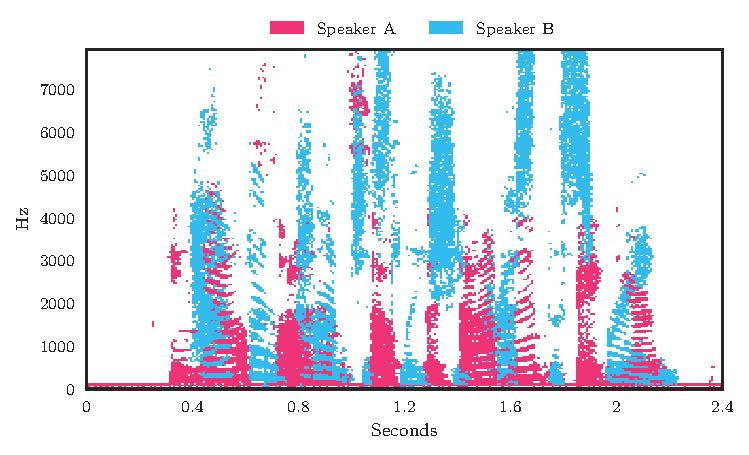
\includegraphics[width=0.8\textwidth]{gfx/dominance_map_speakers.pdf}}%
\hspace{0.2\textwidth} % seperation
\subcaptionbox[Vocal/Accompaniment]{Vocal/Accompaniment}
[1\textwidth]{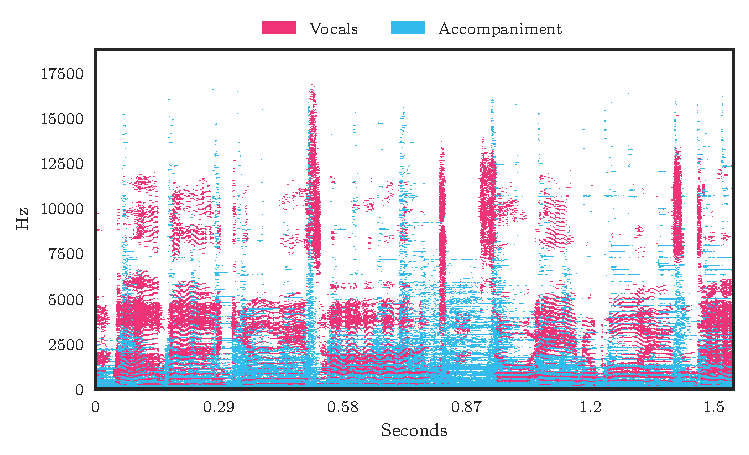
\includegraphics[width=0.8\textwidth]{gfx/dominance_map_vocacc.pdf}}%
\hspace{0.2\textwidth} % seperation
\subcaptionbox[Speech]{Unison}
[1\textwidth]{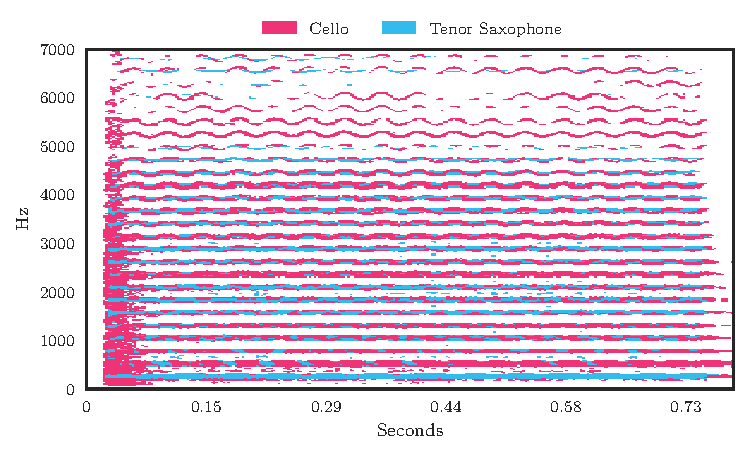
\includegraphics[width=0.8\textwidth]{gfx/dominance_map_unison.pdf}}%
\caption{Predominant source activity, showing the predominant source for each time  frequency entry. Computed using binary masks of each source entry.}
\label{fig:dominance}
\end{figure*}

\begin{figure*}[hb]
\centering
\subcaptionbox[Speech]{Speech}%
[1\textwidth]{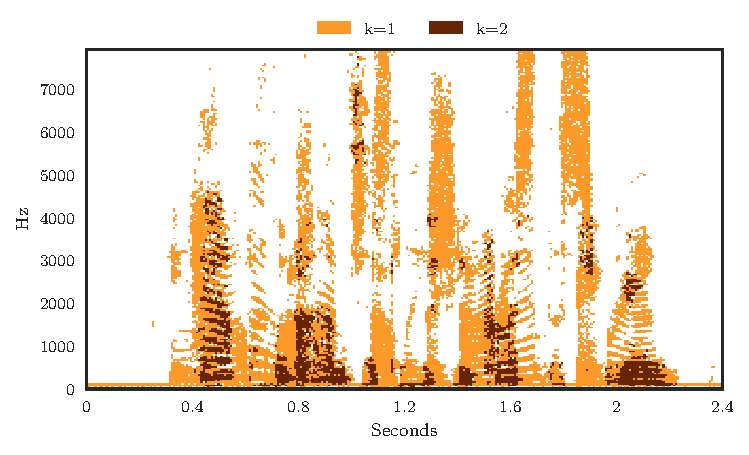
\includegraphics[width=0.8\textwidth]{gfx/count_map_speakers.pdf}}%
\hspace{0.2\textwidth} % seperation
\subcaptionbox[Vocal/Accompaniment]{Vocal/Accompaniment}
[1\textwidth]{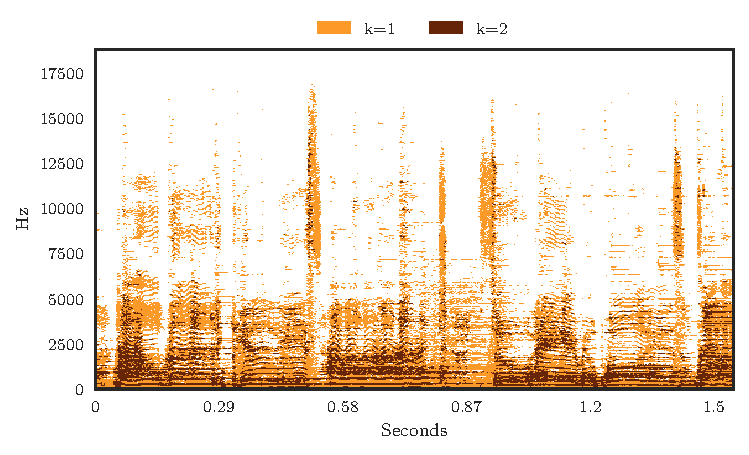
\includegraphics[width=0.8\textwidth]{gfx/count_map_vocacc.pdf}}%
\hspace{0.2\textwidth} % seperation
\subcaptionbox[Unison]{Unison Instruments}
[1\textwidth]{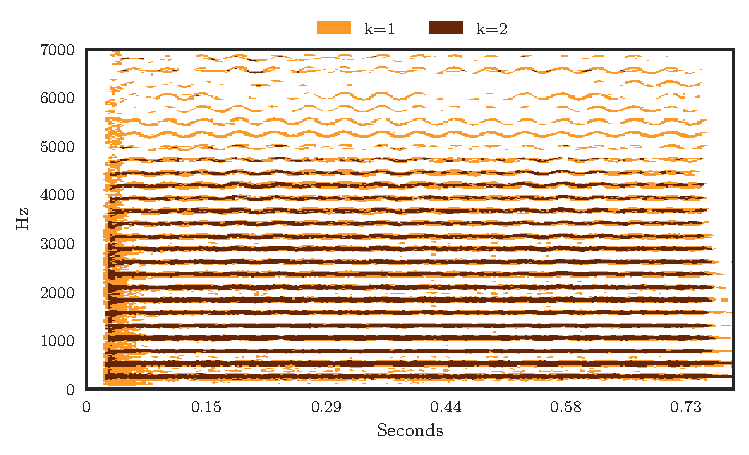
\includegraphics[width=0.8\textwidth]{gfx/count_map_unison.pdf}}%
\caption{Source Count Activity showing the number of sources $k$ for each time frequency entry. Computed using binary masks of each source entry.}
\label{fig:count}
\end{figure*}

To illustrate this, we depict the different scenarios in two complementary figures.
Figure~\ref{fig:dominance} assigns each time-frequency entry to its predominant source.
Figure~\ref{fig:count} depicts the number of active sources (thresholded) of each TF entry.
From these figures, one can see that the overlap of a typical speech mixture is comparable to a music recording where the task is to separate vocals and accompaniment.
If we now compare this to the scenario where sources are fully overlapped as in the unison scenario, almost all TF bins are overlapped, and separation would hardly be possible.
\par
While this is an extreme scenario, it still provides a useful example where common assumptions are violated, and it would facilitate the demand to develop new methods that do not rely so much on these assumptions.
By naïvely observing the time-frequency representation in Figure~\ref{fig:count} closely, we see that the slow spectro-temporal modulations caused by the vibrato are one of the aspects where the two sources differ.
Here, the classical STFT does not provide sufficient separability and representations as in the \emph{modulation spectrogram}, presented by~\cite{greenberg96} may be preferable.
Details about this approach are discussed in Chapter~\ref{cha:unknown}.

\hypertarget{exploiting-slow-modulations}{%
\section{Exploiting Slow Modulations}\label{exploiting-slow-modulations}}

Tempo-spectral modulations occur both in speech and music signals as detailed in Section~\ref{sub:time-variant-audio-signals}.
Exploiting modulations is natural for humans: early research from Zwicker in 1952 focused on the human ability to detect amplitude modulations~\cite{zwicker52}. 
Later, it was shown by Bregman, McAdams, and Fastl in~\cite{mcadams89, bregman90, fastl90} that humans use amplitude modulations to group sources; this concept was called \emph{Common Amplitude Modulation} (CAM).
CAM exploits the fact that harmonics that share the same amplitude modulation across frequency bins are perceived \emph{integrated} as opposed to~\emph{segregated}.
Further, it was shown in~\cite{bacon89} that the ability to detect amplitude modulations can be incorporated into auditory models.
It was then found by Dau in~\cite{dau99} that humans are especially sensitive at low-frequency modulations:

\begin{quote}
``Slow modulations are associated with the perception of rhythm. Samples of running speech, for example, show distributions of modulation frequencies with peaks around 3-4 Hz, approximately corresponding to the sequence rate of syllables~\cite{plomp83}. Results from physiological studies have shown that, at least in mammals, the auditory cortex seems to be limited in its ability to follow fast temporal changes.''
\end{quote}

Dau proposed a model that mimics the ability to detect modulation patterns and pointed out applications to improve the perception for hearing-impaired listener or speech intelligibility.
\par
Previously, research has addressed a variety of tasks of processing and analysis in the context of modulations.
In the following, we give an overview of existing work focussed on analysis and separation of modulated sounds.

\subsection{Analysis}

%lets start with speech
In speech, techniques using modulation patterns improved applications such as speech  discrimination~\cite{mesgarani04} or extract spatial acoustic signatures from mixtures~\cite{sukittanon06}.
One way of analyzing amplitude modulations is to use a modulation spectrogram~\cite{greenberg97} which is a frequency-frequency representation of a time domain input signal.
A complete signal representation can be archived by a modulation tensor which holds the modulation spectrograms for each time frame.
Interestingly, Greenberg in~\cite{greenberg97} assumed that ``the energy in the modulation spectrum may be derived from syllabic segmentation'' and from ``the preservation of the portion of the modulation spectrum between 2 and 10 Hz''.
Following this, it was later proved that the detection of modulations improves speech intelligibility~\cite{elhilali03} or automatic speech recognition~\cite{kingsbury98}.
\par
% go to music
Amplitude modulations were also proposed for music tasks. 
Work by Scheirer in~\cite{scheirer99} proposed a method that operates by utilizing common modulation among groups of frequency sub-bands in the auto correlogram domain.
In music, where modulations are predominantly caused by vibrato, frequency modulation is important.
For frequency modulations, however, the modulation spectrogram is less effective, as it would only be able to track the modulation through side-lobes.
Here, a common way to explicitly analyze frequency variations is first to analyze the fundamental frequency and then track the fundamental frequency over time to smoothen out the contour.
An overview of techniques is summarized in~\cite{driedger16}.
The authors of this paper also proposed a novel method to directly estimate the parameters of potential frequency modulations in the time-frequency domain by matching sinusoidal templates.
\par
Disch and Edler proposed in~\cite{disch09} to decompose an audio signal into bandpass signals, each of them parametrically modeled by a sinusoidal carrier and its amplitude and frequency modulation.

\subsection{Processing}

As described in the previous chapter, modulations are used by humans to group and segregate sounds. Viste et al. describes the impact of modulation in~\cite{viste03} as:

\begin{quote}
``harmonic relation, the common onset, offset, amplitude modulation (AM), and frequency modulation (FM). These are all important cues for grouping.''
\end{quote}

It is therefore not surprising that a number of methods exist, that utilize spectro-temporal modulations to separate mixtures. 
These methods were summarized in~\cite{rafii}, starting with one of the first concepts introduced by~\cite{bregman90} as the \emph{common amplitude modulation} ``which exploits that amplitude envelopes of different harmonics of the same source tend to be similar.''
This was later used in models to separate mixtures such as in ~\cite{li07, li09}.\\
Furthermore, common amplitude modulation characteristics was included in the separation scheme in works such as~\cite{cano14}.\\
Wang proposed a technique in~\cite{wang94,wang95} of ``\dots instantaneous and frequency-warped techniques for signal parameterization and source separation, with application to voice separation in music.''\\
Yen et al. proposed in \cite{yen14,yen15} to use spectro-temporal modulation features to decompose ``a mixture using a two-stage auditory model which consists of a cochlear module \cite{chi05} and cortical module \cite{chi99}.'' (from~\cite{rafii}.\\
Virtanen made use of sinusoidal modeling \cite{virtanen00} to model and separate sources with tempo spectral modulation like vibrato.

In another vein, the source-filter model was deployed to separation sources~\cite{hennequin10}.
An advantage of the source-filter model, as pointed out in~\cite{rafii} is that ``\dots one can dissociate the pitched content of the signal, embodied by the position of its harmonics, from its TF envelope which describes where the energy of the sound lies.''

\section{Summary}

Modulations play an essential role in audio signals. 
However, past research was mainly focused on single notes and not on overlapped sounds.
It is, therefore, to be investigated if scenarios with severe overlap can utilize modulations as well: parameterization of modulation characteristics of a single source is difficult when only the mixture can be observed. 
It is known~\cite{salamon13} that the extraction of the fundamental frequency in a mixture is challenging. 
The reason is that crossing partials are a challenging problem for sinusoidal modeling~\cite{viste03}. 
Also if tracking of them would work correctly, evaluation of robustness and accuracy is hardly possible when the reference data is annotated with human precision.
Furthermore, representations like modulation spectrograms only cover amplitude modulations, whereas general modulation patterns (AM/FM, timbre modulation) cannot be covered.
\par
In the next two chapters, we address utilizing the modulations of sources for separation tasks; either via prior knowledge (known) or by operating blindly (unknown).
% \chapter{Datasets}
\label{cha:datasets}

In the previous chapter, we presented the fundamentals of highly overlapped audio signals.
To study these signals in a reproducible manner, suitable data is of paramount importance since many methods rely on audio datasets for development and evaluation.
Often, suitable audio material is not publicly available, in the case of music, often because of restrictive copyright laws. 
Therefore, in the past, many academic endeavors were focussed on assembling such precious data. 
In fact, major conferences within the audio community value datasets contributions as important as the development of novel methods that often was enabling this research. 
In the following sections, we present three datasets which we helped creating.
Each of the three datasets is released in public domain and aim to fill specific needs and are used in subsequent experiments throughout this thesis.

\section{Unison Mixtures}
\label{sec:unison_dataset}

\marginpar{
  Parts of this this section were previously published in~\cite{stoter14}.
}

In speech, it is common to mix clean speech and noise~\cite{varga93} or different clean speech signals such as~\cite{garofolo93} to generate mixtures.
By contrast, the conversational aspect of human-to-human communication is lost.
Compared to speech, musical content usually does share familiar orchestration, can hardly be superimposed randomly and the summing of isolated random notes from musical instrument databases does not reflect musical performances.
On the positive side, there are use-cases for single note datasets such as for evaluation of fundamental frequency estimation algorithms or the detection of instruments.
Furthermore, single note datasets allow using the data to synthesize musical score as long as the recordings have enough variance of expressions.
It also allows to quickly generate a large number of mixtures using randomly permuted mixtures, fostering applications in machine learning.

As an exception compared to other music scenarios, when all instruments play~\emph{in unison}, single note datasets are appropriate to approximate real mixtures:

\begin{itemize}
  \item A random summation of multiple instruments playing the same note does not necessarily differ from realistic unison mixture.
  \item When notes are played with vibrato, having access to the individual modulation patterns can help to study the influence of modulations systematically.
  \item Unison mixtures are part of many classical compositions, to extend the timbre of a note.
\end{itemize}

\par
To create a dataset, we could use existing single note datasets such as the \emph{Univ. of Iowa Musical Instrument Sample Database}\footnote{\url{http://theremin.music.uiowa.edu/index.htm}}, created from acoustic recording sessions.
However, to better study the influence of vibrato we require extended control over certain parameters such as note duration, vibrato duration, exact fundamental frequency, vibrato rate, vibrato extend, reproducibility, loudness or expression.
\par
As mentioned in previous chapters, vibrato techniques vary across instruments. Instruments such as violin and tenor sax are known for its distinct frequency modulations~\cite{gilbert05}.
Other instruments such as the English horn and the flute are more close to amplitude modulations.
\par
We, therefore, generated the notes using a software sampler\footnote{\textsc{Vienna Symphonic Library}: \url{https://vsl.co.at}} which allows us to control the parameters such as the vibrato.
All our test stimuli have a duration of three seconds.
Items were equalized in loudness by using an iterative calculation of the loudness algorithm of the time-varying Zwicker model~\cite{zwicker13}. 
We used an implementation released in~\cite{genesis12}. 
\par
We rendered 29 notes of C4, resulting in 841 unique unison instrument mixtures per pitch class.
An excerpt of the instruments is listed in Table~\ref{tab:testset}.
The dataset is available from~\cite{oss_unison}.

\begin{table}
\begin{center}
\footnotesize
\begin{tabular}{ l l l}
  Instrument & Vibrato &  MIDI \# \\
  \hline
  Violin & yes & 40 \\
  Viola & yes & 41 \\
  Violon Cello & yes & 42 \\
  Trumpet & no & 56 \\
  Trombone & no & 57\\
  Horn & no & 60  \\
  Bariton Sax & yes & 67 \\
  Oboe & no & 68\\
  Clarinet & no & 71\\
  Flute & yes & 73\\
\end{tabular}
\end{center}
\caption{Selected Instruments from the \emph{Unison Source Separation Dataset}~\cite{oss_unison} as used in~\cite{stoeter14, stoeter16}.}
\label{tab:testset}
\end{table}

To evaluate the level of overlap, we created a small experiment where we computed the average W-disjoint orthogonality \(WDO\) metric for 1000 random combinations of mixtures for different separation scenarios.
It turned out that for speech separation of \(k=2\) speakers, (\(WDO=0.9\)) and for the vocal accompaniment scenario (\(WDO=0.87\)), surprisingly similar even though both scenarios are so fundamentally different.
In the case of two instruments playing in unison, the average WDO is \(0.65\), indicating that a good separation in the time-frequency domain is more challenging, thus making the dataset a useful addition compared to existing scenarios.

% \begin{figure}
% \begin{tikzpicture}
%     \begin{axis}[
%         xlabel=Number of Sources,
%     ylabel=Separability/WDO]
%     % speakers
%     \addplot[color=red,mark=x] coordinates {
%         (2,0.9)
%         (3,0.79)
%         (4,0.69)
%         (5,0.6)
%         (6,0.536)
%         (7,0.462)
%         (8,0.4197)
%         (9,0.352199)
%         (10,0.32)
%   };
%   % single note
%       \addplot[color=blue,mark=x] coordinates {
%         (2,0.928)
%         (3,0.864)
%         (4,0.8)
%         (5,0.77)
%         (6,0.682)
%         (7,0.637)
%         (8,0.592)
%         (9,0.5647)
%         (10,0.5434)
%   };
%   % unison
%     \addplot[color=yellow,mark=x] coordinates {
%         (2,0.626)
%         (3,0.32)
%         (4,0.2)
%         (5,0.13)
%         (6,0.083)
%         (7,0.038)
%         (8,0.025)
%         (9,0.017)
%         (10,0.01)
%     };
%     \end{axis}
% \end{tikzpicture}
% \end{figure}

\section{High Resolution Vibrato Recordings}%
\label{sec:muserc}

\marginpar{
  Parts of this this section were previously published in~\cite{stoeter15acm}.
}

Fundamental frequency \(F0\) estimation of a signal is a common task in audio signal processing with many applications. 
If the $F0$ varies over time, the complexity increases, and it is also more difficult to provide ground truth data for evaluation.

\begin{figure}[h]
  \centering
  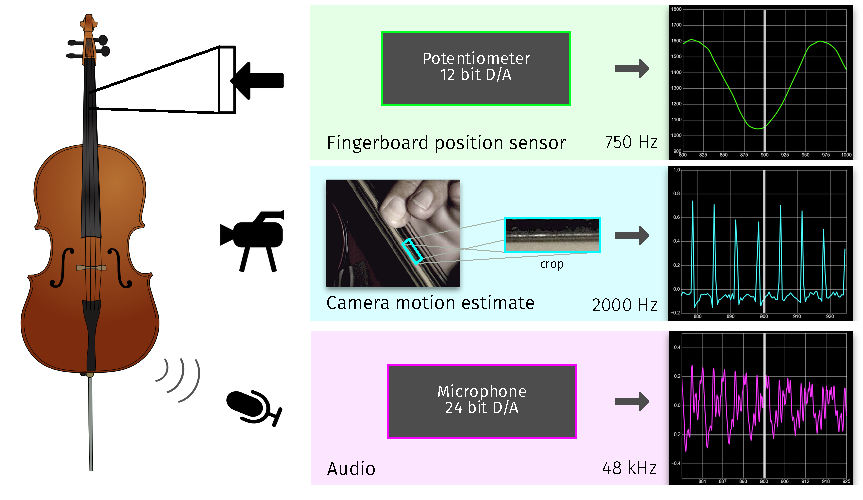
\includegraphics[width=\textwidth]{Chapters/04_Data/figures/teaser.pdf}
  \caption{Overview of the multi-modal data recorded for the proposed dataset.}
\label{fig:teaser_hdf0}
\end{figure}

% from stoter acm
For speech signals, an EGG device (also known as laryngograph) captures the excitation of the human vocal tract. 
This signal is then processed by an $F0$ estimator to generate the ground truth. 
Such a method is accepted in published research because the EGG signal is considered to be easier to process than speech. 
The retrieved F0-trajectory based on the EGG signal is easier to process and the generated annotations are considered as a good ground truth~\cite{pirker11, babacan13}.
Motivated by this, we propose a new data set for musical instruments where we recorded a violin cello with extra sensors on the fretboard in addition to audio and video.
We made use of multiple sensors to capture the most relevant processes involved in creating time-varying output signals as depicted in Figure~\ref{fig:teaser_hdf0}.
We included sensor recordings capturing the finger position on the fingerboard which is converted into an instantaneous frequency estimate.
We also included high-speed video camera data to capture excitations from the string at 2000 fps.
Recording video data was inspired by the work of Davis et.\ al.\ in~\cite{Davis2014VisualMic} presenting a ``visual microphone'' which is able to observe sound solely with a camera, pointing to objects in the sound field. 
\par
In the proposed dataset we chose the violin cello for the following reasons: (1) vibrato is used as a common style for expression, (2) there is an observable physical relationship between frequency modulation and vibrato, and (3) the instrument is large enough to embed sensors to capture the vibrato. The properties of the cello are studied by research in acoustics~\cite{woodhouse04, woodhouse99}.
\par
To capture significant aspects of the cello while being played by a musician, we focus on three main observations: (1) Excitation caused by the moving bow; (2) the vibrating string, and (3) the finger, controlling the string length by rolling it on the fingerboard.
The main focus of the recordings is to analyze vibrato playing style. Since it is common that vibrato characteristics differ from musician to musician, all recordings were performed by two musicians. One is a professional cellist with 30 years of experience in a symphonic orchestra\footnote{\url{http://www.bambergerstreichquartett.de/de/Das_Quartett/Karlheinz_Busch}}.
The other recording was done by the author of this thesis, who has less than 1 hour per week of practice.
\par
Due to the width of fingerboard sensors and the attached cables we were able to equip two strings (G and A) allowing to record pitches ${G2, D3, D^\sharp3, E3, A3, B3, C4, C^\sharp4}$ from both musicians (see the middle part of Figure~\ref{fig:teaser_hdf0}).
\par
The dataset includes time synchronous fingerboard positions and high-speed camera recordings. 
The derived motion estimates show similarity to the EGG signals used in speech. 
The slowest feature rate of the set is 750 Hz, which enables to evaluate $F0$ estimators with high temporal resolution. 
\par
In~\cite{stoeter15acm}, we also showed how to derive high resolution $F0$ contours from the data which can be used to improve $F0$ estimators or help to analyze playing styles in recordings, usually relying on conventional $F0$ estimators based on the audio signal~\cite{mellody2000time}. 
By using sensor data samples from our test set, researchers get more robust and detailed data to compute features like mean vibrato frequency. 
Further, it can be used for synthesizers to add a natural vibrato by using the sensor data as a modulation source.
\par
The resulting test set yields in $148$ recorded notes after removal of some notes due to errors in the sensor recordings.
By making this dataset public domain~\cite{oss_muserc} and including the raw recordings, we believe other researchers can benefit from the data and possibly generate their own derived data.

\section{Multitrack Music Recordings}%
\label{sec:multitrack}

For the evaluation source separation, it is important 
 Signal Separation Evaluation Campaign (SiSEC) is a publicly organized benchmark to assess the performance of source separation systems~\cite{sisec13, ono15, liutkus17, stoeter18sisec}.
To evaluate participating methods, multitrack data is required, containing the true sources.

``For professionally-produced or recorded music, the separated sources are often either unavailable or private. Indeed, they are considered amongst the most precious assets of right holders, and it is challenging to find isolated vocals and accompaniment of professional bands that are freely available for the research community to work on without copyright infringements.
In this context, the development of datasets for music separation was a long process. 
In early times, it was common for researchers to test their methods on private data. 
To the best of our knowledge, the first attempt at releasing a public dataset for evaluating vocals and accompaniment separation was the Music Audio Signal Separation (MASS) dataset~\cite{MTGMASSdb}.
It strongly boosted research in the area, even if it only featured 2.5 minutes of data. The breakthrough was made possible by some artists which made their mixed-down audio, as well as its constitutive stems (unmixed tracks), available under open licenses such as Creative Commons, or authorized scientists to use their material for research.''~\cite{rafii}.
% 
``The MASS dataset formed the core content of the early Signal Separation Evaluation Campaigns (SiSEC) \cite{vincent09}.''~\cite{rafii}.
``For a long time, vocals separation methods were very demanding computationally and it was already considered extremely challenging to separate excerpts of only a few seconds.''~\cite{rafii}.

``In the following years, new datasets were proposed that improved over the MASS dataset in many directions. 
We briefly describe the most relevant ones below:

\begin{itemize}[leftmargin=*]
    \item The QUASI dataset was proposed to study the impact of different mixing scenarios on the separation quality. It consists of the same tracks as in the MASS dataset, but kept the full length and mixed by professional sound engineers.
    \item The MIR-1K~\cite{hsu10} and iKala~\cite{chan15} datasets were the first attempts to scale vocals separation up. They feature a higher number of samples (1000) than the previously available datasets. However, they consist of mono signals of very short and amateur karaoke recordings.
    \item The ccMixter~\cite{liutkus142} dataset was proposed as the first dataset to feature many full-length stereo tracks. Each one comes with vocals and an accompaniment source. Although it is stereo, it often suffers from simplistic mixing of sources, making it unrealistic in some aspects.
    \item MedleyDB~\cite{bittner14} has been developed as a dataset to serve many purposes in music information retrieval. It consists of more than 100 full-length recordings, with all their constitutive sources. It is the first dataset to provide such a large amount of data to be used for audio separation research (more than 7 hours). Among all the material present in that dataset, 63 tracks feature singing voice.
    \item DSD100~\cite{liutkus17} was presented for SiSEC 2016. It features 100 full-length tracks originating from the 'Mixing Secret' Free Multitrack Download Library of the Cambridge Music Technology, which is freely usable for research and educational purposes.''
    The dataset consists of four predefined categories: \emph{bass, drums, vocals}, and \emph{other}. An extended version, merging MedleyDB and DSD100 was recently released as MUSDB18~\cite{rafii17, stoeter18sisec}
\end{itemize}

\begin{table*}[htbp]
	\centering
	\caption{Summary of datasets available for lead and accompaniment separation. Tracks without vocals were omitted in the statistics.}
	\label{tab:datasets}
		\begin{tabular}{|l l l l l l l|}
			\hline
			\textbf{Dataset} & \textbf{Year} & \textbf{Reference(s)} & \textbf{Tracks} & \textbf{Track duration (s)} & \textbf{Full/stereo?}\\
			\hline
			MASS & 2008 & \cite{MTGMASSdb} & 9 & $16 \pm 7$ & no / yes \\
			MIR-1K & 2010 & \cite{hsu10} & 1,000 & $8 \pm 8$ & no / no \\
			QUASI & 2011 & \cite{liutkus11,vincent12} & 5 & $206 \pm 21$ & yes / yes \\
			ccMixter & 2014 & \cite{liutkus142} & 50 & $231 \pm 77 $ & yes / yes \\
			MedleyDB & 2014 & \cite{bittner14} & 63 & $206 \pm 121$ & yes / yes \\
			iKala & 2015 & \cite{chan15} & 206 & 30 & no / no \\
			DSD100 & 2015 & \cite{ono15} & 100 & $251 \pm 60$ & yes / yes \\
      MUSDB18 & 2017 & \cite{rafii17} & 150 & $236 \pm 95$ & yes / yes \\
			\hline
		\end{tabular}
\end{table*}

% from \cite{stoeter18sisec}
All items are full-length tracks, enabling the handling of long-term musical structures, and the evaluation of quality over silent regions for sources. All signals are stereo and mixed using professional digital audio workstations, thus representative of real application scenarios. All signals are split  into four predefined targets: bass, drums, vocals and other. This promotes automation of the algorithms. Many musical genres are represented: jazz, electro, metal, etc. It is split into a training (100 tracks, 6.5 h) and a test set (50 tracks, 3.5 h), for the design of data-driven methods.


Over the years, DSD100/MUSDB18 became one of the most used datasets for source separation. 
The dataset is still small in comparison to machine learning sets from vision such as~\ref{}, but it proved to be large enough to help DNN-based methods to reach breakthrough results in source separation~\cite{stoeter18sisec}.
\par
Working with multitrack audio files can be cumbersome due to its hierarchical structure that needs to be parsed.
For that purpose, we developed a software toolbox for Python that permits the straightforward processing of the DSD100 dataset. This software is open source and was publicly broadcasted so as to allow the participants to run the evaluation themselves\footnote{\url{github.com/faroit/dsdtools}}.
\par
This package integrates with existing Python code, thus makes it easy to participate in the SISEC MUS tasks. The core of this package is calling a user-provided function that separates the mixtures from the DSD into several estimated target sources.

% TODO: add musdb example
% \begin{code}
% \captionof{listing}{Full working code example to parse the full DSD100~\cite{liutkus17} dataset as \emph{NumPy} arrays and write out estimates (here: the mixture) into a predefined estimates directory.}
% \begin{minted}{python}
% import dsdtools

% def my_function(track):
%     estimates = {
%         'vocals': track.audio,
%         'accompaniment': track.audio,
%     }
%     return estimates

% dsd = dsdtools.DB(root_dir="./Volumes/Data/dsdtools")
% dsd.run(my_function, estimates_dir="path/to/estimates")
% \end{minted}
% \label{code:c-code}
% \end{code}

All details of this accompanying software tools may be found on its dedicated website\footnote{\url{https://sigsep.github.io}}.
% \chapter{Separation by Known Modulation}
\label{cha:known}

% TODO: add \cite{smaragdis08} for shift invariant NMFs and discuss the differences.

For many source separation methods it is common to assume that the spectral harmonics are not fully overlapped.
In turn, this assumption is exploited in methods such as non-negative matrix factorization (NMF) to approximate the mixture from a lower-rank decomposition in an unsupervised way.
Still, in order to improve separation quality, researchers imposed additional constraints based on  prior information about the sources in their algorithms~\cite{ozerov12}.
The extent of such meta information very often depends on 
the availability the data.
One example of an informed source separation systems is described by Ewert and M\"uller \cite{ewert12}.
They proposed to incorporate the note pitch and onset information of the musical score, encoded in a MIDI file, synchronized to the audio, to improve the separation result.
% end converted from dafx
\par
In the case of highly overlapped signals such as unison mixtures, the score is less useful since unison mixtures share the same note pitch.
Instead, in this chapter, we want evaluate the use of fundamental frequency estimates of the source to be extracted.
In fact, there has been extensive research on separation using the fundamental frequency in music separation.
The first option is to re-synthesize the source using a sinusoidal model which was studied in a large number of methods\footnote{For a detailed overview, I refer the reader to Section III A of~\cite{rafii})}.
However, sinusoidal synthesis suffers from a typical \textit{metallic} sound quality, which is mostly due to discrepancies between the estimated excitation signals of the lead signal compared to the ground truth, we decided to take an alternative approach which is to exploit harmonicity in another way, by filtering out everything from the mixture that is not located close to the detected harmonics.
In the past, many related work was focus on this paradigm, a procedure as it turned out to be a common task in source separation systems. 
Before I present our proposed method in the next section, the following gives an overview existing methods ins this field.

\subsection*{Related Work}

\marginpar{This subsection is based on the work that has been published in~\cite{rafii} as a joint effort to review the state-of-the-art of lead/accompaniment separation.}

% from zafar
E.g. Li and Wang proposed to use a vocal/non-vocal classifier and a predominant pitch detection algorithm \cite{li06, li07}. They first detected the singing voice by using a spectral change detector \cite{duxbury03} to partition the mixture into homogeneous portions, and GMMs on MFCCs to classify the portions as vocal or non-vocal. Then, they used the predominant pitch detection algorithm in~\cite{li05} to detect the pitch contours from the vocal portions, extending the multi-pitch tracking algorithm in~\cite{wu03}. Finally, they extracted the singing voice by decomposing the vocal portions into TF units and labeling them as singing or accompaniment dominant, extending the speech separation algorithm in \cite{hu02}.
\par
Han and Raphael proposed an approach for de-soloing a recording of a soloist with an accompaniment given a musical score and its time alignment with the recording \cite{han07}. They derived a mask \cite{roweis01} to remove the solo part after using an EM algorithm to estimate its melody, that exploits the score as side information.
\par
Hsu et al. proposed an approach which also identifies and separates the unvoiced singing voice \cite{hsu08,hsu10}. Instead of processing in the STFT domain, they use the perceptually motivated Gammatone filter-bank as in~\cite{hu02,li07}. They first detected accompaniment, unvoiced, and voiced segments using an HMM and identified voice-dominant TF units in the voiced frames by using the singing voice separation method in \cite{li07}, using the predominant pitch detection algorithm in \cite{dressler062}. Unvoiced-dominant TF units were identified using a GMM classifier with MFCC features learned from training data. Finally, filtering was achieved with spectral subtraction~\cite{scalart96}.
\par
Raphael and Han then proposed a classifier-based approach to separate a soloist from accompanying instruments using a time-aligned symbolic musical score \cite{raphael08}. They built a tree-structured classifier \cite{breiman84} learned from labeled training data to classify TF points in the STFT as belonging to solo or accompaniment. They additionally constrained their classifier to estimate masks having a connected structure.
\par
Cano et al. proposed various approaches for solo and accompaniment separation. In~\cite{cano09}, they separated saxophone melodies from mixtures with piano and/or orchestra by using a melody line detection algorithm, incorporating information about typical saxophone melody lines. In~\cite{grollmisch11,dittmar12,cano12}, they proposed to use the pitch detection algorithm in~\cite{dressler11}. Then, they refined the fundamental frequency and the harmonics, and created a binary mask for the solo and accompaniment. They finally used a post-processing stage to refine the separation. In \cite{cano13}, they included a noise spectrum in the harmonic refinement stage to also capture noise-like sounds in vocals. In \cite{cano14}, they additionally included common amplitude modulation characteristics in the separation scheme.
\par
Bosch et al. proposed to separate the lead instrument using a musical score \cite{bosch12}. After a preliminary alignment of the score to the mixture, they estimated a score confidence measure to deal with local misalignments and used it to guide the predominant pitch tracking. Finally, they performed low-latency separation based on the method in \cite{marxer12}, by combining harmonic masks derived from the estimated pitch.
\par
Vaneph et al. proposed a framework for vocal isolation to help spectral editing \cite{vaneph16}. They first used a voice activity detection process based on a deep learning technique \cite{Leglaive15}. Then, they used pitch tracking to detect the melodic line of the vocal and used it to separate the vocal and background, allowing a user to provide manual annotations when necessary.

\section{F0 Variation Informed Separation}
\label{sub:frequency_modulation}

\marginpar{This section is based on the work published in 2014 together with my collegue Stefan Bayer ~\cite{stoeter14}. The publication is based on my original idea.}

Frequency modulation caused by vibrato is a very common playing style for string instruments but also for woodwind and brass instruments.
Vibrato is an effect that is well studied especially in musicology, for more information the reader is referred to the overview given in the Section~\ref{sub:time-variant-audio-signals}.
Performers are able to perform a vibrato in the same way when repeating a performance~\cite{fletcher01}.
For example, vibrato rates vary across different instruments.
In~\cite{macleod06} the vibrato width (frequency deviation) was found to be significantly different between violinists and violists performers.
This can be exploited in source separation scenarios.
\par
However, in the case of a NMF, it lacks the ability to model time varying frequencies since the $\mathbf{W}$ matrix is fixed.
Several extensions for NMF have been proposed to improve the decomposition quality.
Hennequin et al. proposed in \cite{hennequin11} a frequency dependent activations matrices, whereas Smaragdis et al. developed a variant of the NMF in ~\cite{smaragdis08} which is invariant to frequency shifts.
Another approach is to model the spectral pattern changes by Markov chains \cite{nakano10}. All these approaches attempt to model the non-stationary effects within the decomposition model.
In this work, instead, we propose a method that increases the stationarity of the signal in preprocessing step and then use the standard separation like NMF for the decomposition.\\

\subsection{Time Warping}
\label{sub:time_warping}
% Content by Stefan Bayer
The idea is to make use of \emph{time-warping} which refers to a mapping of the linear time scale $t$ to a warped time scale $\tau$ via a mapping function $\tau=w(t)$.
To ensure a unique mapping, the mapping function needs to be strictly increasing.
For the discrete time case the mapping can be achieved by a time-varying re-sampling of the linear (i.e. regularly sampled) time signal under consideration.
The instantaneous sampling frequency then corresponds to the first derivative of
the mapping function. Although the mapping can be done from any time-span
$I$ on the linear time scale to any time span $J$ on the warped time scale, in
the discrete time case it is advantageous to have the same number of samples
in the linear and warped time domain. This ensures that the average sampling
frequency is the same in both domains. Such time-warping approaches have already
been proposed for different purposes such as transform-based audio coding
\cite{edler09}. As in these applications, we derive the mapping function from
the varying instantaneous fundamental frequency in such a manner that the variation of the frequency is
reduced or removed. To be more precise the actual information needed is not
the absolute instantaneous fundamental frequency but only its change over time.
The discrete time warp map $w[n]$ is then simply the scaled sum of the relative
frequencies $f[n]$:
\begin{equation}
w[n]=N \frac{\sum^n_{l=0}{f[l]}}{\sum^N_{k=0}{f[k]}}  \qquad 0\leq n<N,
\end{equation}
where $N$ being the number of samples of the signal under consideration.
From the requirements for the mapping function it follows that the relative
frequency $f[n]$ has to be positive at all instants and preferably should not
exhibit large jumps.
For the mapping from linear to warped time now the linear domain sample points
$s[\nu]$ for the regularly spaced samples $x[\nu]$ in the warped domain are
found by inverting $w[n]$. These sample points are then used to re-sample the linear time
domain samples $x[n]$ to the warped time domain samples $x[\nu]$, in our case
by employing an 128 times oversampled FIR low-pass filter. This processing leads to a sampling rate contour which is proportional to the pitch contour. Or in other words, a fixed number of samples are obtained in each period of the signal with the varying fundamental frequency. Mutatis mutandis the sample points $s[\nu]$ can be used for the re-sampling from warped time domain to linear time domain. \\

In this work, the time-warping was done globally over the full lengths of the
signals under consideration. The globally time-warped sample sequence
was then used in the further processing steps. In Figure~\ref{fig:timewarptime} we show the results of the warping process in the time domain. \\

The use of time variable rate sampling was first proposed by~\cite{wulich92} which used this method to analyze FM signals.

A similar approach using frequency modulation to separate a harmonic
source from a mixture was proposed in \cite{wang95}. Here the
individual lines are demodulated to the base band using a combined frequency
tracking/demodulation approach. The difference to our approach is that first
the absolute instantaneous frequency for every harmonic line has to be known
instead of a relative frequency that is common to all harmonic lines of a single
source. This relative frequency might be obtained easier than its
absolute value for a mixed signal. Secondly every harmonic line has to be individually frequency demodulated while in our approach the full signal is frequency demodulated in one algorithmic step.\\

\subsection{Separation} % (fold)
\label{sub:pitch_variation_informed_source_separation}

With the ability to remove the frequency modulation from a signal we can then include this system in a source separation system to address the non-stationarity issues of NMF based approaches. 
Figure~\ref{fig:warpingdemo} shows how this system works on a purely harmonic FM signal mixture. 
Plots (a) and (b) show the two input signals which are linearly mixed (c). 
For each source the warp contour needs to be calculated. 
The mixture is then warped with F0 variation estimates of source 1 (d) and source 2 (e). 
The actual separation/filtering of the sources is then done by using NMF which is not shown here. 
To separate the components from the warped mixture we used NMF on a STFT computed with a long DFT (about 0.5 s). 
We applied NMF fully unsupervised clustering components based on tonality of $\textbf{W}$ by using a spectral flatness measure~\cite{gray74}. The separated signals (f) and (g) then need to be warped back into the original time domain resulting in (h) and (i).

It is important to clarify that this approach would not be able to separate two modulating instruments playing in unison without having prior knowledge about the individual modulation functions. Although a F0 variation estimate might be difficult to achieve in a mixture, our approach shows that such a system could work if that estimate is accurate.

\begin{figure}[t]
\begin{tikzpicture}
    \node (inputmeta) [inner sep=0pt] {
        \begin{tikzpicture}
            \node (input) [inner sep=0pt] {\resizebox{0.25\columnwidth}{!}{% This file was created by matlab2tikz v0.4.6 (commit 5265feba1c823c039fc4c4d3e94b826f57582f42) running on MATLAB 7.12.
% Copyright (c) 2008--2014, Nico Schlömer <nico.schloemer@gmail.com>
% All rights reserved.
% Minimal pgfplots version: 1.3
% 
% The latest updates can be retrieved from
%   http://www.mathworks.com/matlabcentral/fileexchange/22022-matlab2tikz
% where you can also make suggestions and rate matlab2tikz.
% 
\begin{tikzpicture}

\begin{axis}[%
width=6.01339838214984in,
height=4.0in,
scale only axis,
xmin=100,
xmax=800,
ymin=0.45,
ymax=1.55,
ticks=none,
xticklabels={\empty}
]
\addplot [color=alturquisedark,solid,forget plot, line width=4pt]
  table[row sep=crcr]{1	0.808658283817458\\
2	0.805397831374914\\
3	0.802147102164398\\
4	0.798906258607479\\
5	0.795675462631829\\
6	0.792454875663097\\
7	0.789244658616792\\
8	0.786044971890382\\
9	0.782855975355114\\
10	0.779677828348103\\
11	0.776510689664449\\
12	0.773354717549147\\
13	0.770210069689259\\
14	0.76707690320611\\
15	0.763955374647261\\
16	0.760845639978889\\
17	0.757747854577816\\
18	0.754662173223827\\
19	0.751588750092002\\
20	0.74852773874486\\
21	0.745479292124817\\
22	0.742443562546498\\
23	0.739420701689087\\
24	0.736410860588824\\
25	0.733414189631408\\
26	0.730430838544512\\
27	0.727460956390244\\
28	0.724504691557784\\
29	0.721562191755921\\
30	0.718633604005635\\
31	0.715719074632877\\
32	0.712818749261081\\
33	0.709932772804078\\
34	0.707061289458689\\
35	0.704204442697592\\
36	0.701362375262222\\
37	0.698535229155502\\
38	0.695723145634814\\
39	0.692926265205014\\
40	0.690144727611258\\
41	0.68737867183215\\
42	0.684628236072749\\
43	0.681893557757633\\
44	0.679174773524096\\
45	0.67647201921528\\
46	0.673785429873407\\
47	0.67111513973299\\
48	0.66846128221419\\
49	0.665823989916116\\
50	0.663203394610163\\
51	0.660599627233537\\
52	0.658012817882568\\
53	0.655443095806328\\
54	0.652890589400128\\
55	0.650355426199063\\
56	0.647837732871752\\
57	0.645337635213875\\
58	0.642855258141954\\
59	0.640390725687165\\
60	0.637944160989014\\
61	0.635515686289296\\
62	0.633105422925943\\
63	0.630713491326936\\
64	0.628340011004342\\
65	0.625985100548311\\
66	0.623648877621161\\
67	0.621331458951467\\
68	0.619032960328285\\
69	0.616753496595327\\
70	0.614493181645233\\
71	0.612252128413889\\
72	0.61003044887475\\
73	0.607828254033297\\
74	0.605645653921464\\
75	0.603482757592108\\
76	0.60133967311365\\
77	0.599216507564572\\
78	0.597113367028109\\
79	0.595030356587007\\
80	0.592967580318164\\
81	0.59092514128749\\
82	0.588903141544797\\
83	0.586901682118598\\
84	0.584920863011151\\
85	0.582960783193424\\
86	0.581021540600124\\
87	0.579103232124888\\
88	0.57720595361533\\
89	0.575329799868343\\
90	0.573474864625326\\
91	0.57164124056748\\
92	0.569829019311224\\
93	0.568038291403584\\
94	0.566269146317685\\
95	0.564521672448248\\
96	0.562795957107244\\
97	0.561092086519448\\
98	0.559410145818167\\
99	0.557750219041032\\
100	0.556112389125712\\
101	0.554496737905817\\
102	0.552903346106844\\
103	0.551332293342053\\
104	0.549783658108592\\
105	0.54825751778349\\
106	0.546753948619823\\
107	0.545273025742942\\
108	0.543814823146646\\
109	0.542379413689543\\
110	0.540966869091389\\
111	0.539577259929491\\
112	0.538210655635209\\
113	0.536867124490468\\
114	0.535546733624356\\
115	0.534249549009748\\
116	0.532975635460043\\
117	0.53172505662591\\
118	0.530497874992085\\
119	0.529294151874305\\
120	0.528113947416178\\
121	0.526957320586228\\
122	0.525824329174931\\
123	0.524715029791809\\
124	0.52362947786265\\
125	0.522567727626684\\
126	0.521529832133895\\
127	0.520515843242402\\
128	0.519525811615805\\
129	0.518559786720707\\
130	0.517617816824221\\
131	0.516699948991549\\
132	0.515806229083653\\
133	0.514936701754948\\
134	0.514091410451078\\
135	0.513270397406733\\
136	0.512473703643558\\
137	0.511701368968091\\
138	0.510953431969767\\
139	0.510229930019018\\
140	0.509530899265368\\
141	0.508856374635656\\
142	0.508206389832282\\
143	0.50758097733151\\
144	0.506980168381876\\
145	0.506403993002593\\
146	0.505852479982065\\
147	0.505325656876465\\
148	0.504823550008326\\
149	0.504346184465247\\
150	0.503893584098644\\
151	0.503465771522538\\
152	0.503062768112441\\
153	0.502684594004284\\
154	0.50233126809341\\
155	0.502002808033628\\
156	0.501699230236335\\
157	0.501420549869693\\
158	0.501166780857875\\
159	0.500937935880363\\
160	0.50073402637132\\
161	0.500555062519015\\
162	0.500401053265319\\
163	0.50027200630525\\
164	0.500167928086598\\
165	0.500088823809596\\
166	0.500034697426661\\
167	0.500005551642202\\
168	0.500001387912477\\
169	0.500022206445525\\
170	0.500068006201156\\
171	0.500138784890999\\
172	0.500234538978623\\
173	0.500355263679705\\
174	0.500500952962277\\
175	0.500671599547022\\
176	0.500867194907642\\
177	0.501087729271279\\
178	0.501333191619008\\
179	0.501603569686386\\
180	0.501898849964063\\
181	0.50221901769846\\
182	0.502564056892501\\
183	0.502933950306423\\
184	0.50332867945862\\
185	0.503748224626586\\
186	0.50419256484789\\
187	0.504661677921216\\
188	0.50515554040749\\
189	0.505674127631043\\
190	0.506217413680829\\
191	0.506785371411753\\
192	0.507377972445988\\
193	0.507995187174427\\
194	0.508636984758149\\
195	0.509303333129941\\
196	0.509994198995941\\
197	0.510709547837263\\
198	0.511449343911741\\
199	0.512213550255717\\
200	0.513002128685876\\
201	0.513815039801161\\
202	0.514652242984737\\
203	0.515513696406036\\
204	0.516399357022823\\
205	0.517309180583359\\
206	0.518243121628626\\
207	0.519201133494559\\
208	0.520183168314427\\
209	0.521189177021188\\
210	0.522219109349949\\
211	0.523272913840501\\
212	0.524350537839838\\
213	0.525451927504847\\
214	0.526577027804974\\
215	0.527725782524941\\
216	0.528898134267618\\
217	0.530094024456839\\
218	0.531313393340348\\
219	0.532556179992797\\
220	0.533822322318764\\
221	0.535111757055873\\
222	0.536424419777945\\
223	0.537760244898237\\
224	0.539119165672692\\
225	0.540501114203283\\
226	0.541906021441432\\
227	0.5433338171914\\
228	0.544784430113867\\
229	0.54625778772944\\
230	0.547753816422295\\
231	0.549272441443879\\
232	0.550813586916577\\
233	0.552377175837587\\
234	0.553963130082724\\
235	0.555571370410293\\
236	0.557201816465118\\
237	0.558854386782522\\
238	0.560528998792359\\
239	0.562225568823221\\
240	0.563944012106549\\
241	0.565684242780896\\
242	0.567446173896233\\
243	0.569229717418258\\
244	0.571034784232816\\
245	0.572861284150351\\
246	0.574709125910407\\
247	0.576578217186184\\
248	0.578468464589179\\
249	0.580379773673808\\
250	0.582312048942145\\
251	0.58426519384873\\
252	0.586239110805301\\
253	0.588233701185777\\
254	0.590248865331134\\
255	0.592284502554341\\
256	0.594340511145483\\
257	0.596416788376798\\
258	0.598513230507758\\
259	0.600629732790362\\
260	0.602766189474273\\
261	0.604922493812144\\
262	0.607098538064978\\
263	0.60929421350742\\
264	0.611509410433309\\
265	0.613744018161066\\
266	0.615997925039258\\
267	0.618271018452201\\
268	0.620563184825538\\
269	0.622874309631946\\
270	0.62520427739684\\
271	0.627552971704182\\
272	0.62992027520224\\
273	0.632306069609481\\
274	0.634710235720515\\
275	0.637132653411953\\
276	0.639573201648526\\
277	0.642031758489082\\
278	0.644508201092615\\
279	0.647002405724539\\
280	0.649514247762719\\
281	0.652043601703831\\
282	0.654590341169574\\
283	0.657154338912925\\
284	0.659735466824629\\
285	0.662333595939486\\
286	0.664948596442836\\
287	0.667580337677079\\
288	0.670228688148137\\
289	0.672893515532067\\
290	0.675574686681654\\
291	0.678272067633103\\
292	0.680985523612669\\
293	0.683714919043425\\
294	0.686460117552076\\
295	0.689220981975659\\
296	0.69199737436854\\
297	0.694789156009197\\
298	0.697596187407184\\
299	0.700418328310156\\
300	0.703255437710743\\
301	0.70610737385375\\
302	0.708973994243168\\
303	0.711855155649226\\
304	0.714750714115695\\
305	0.717660524966959\\
306	0.720584442815283\\
307	0.723522321568117\\
308	0.726474014435323\\
309	0.72943937393656\\
310	0.732418251908622\\
311	0.735410499512896\\
312	0.738415967242724\\
313	0.741434504930919\\
314	0.744465961757259\\
315	0.74751018625601\\
316	0.750567026323541\\
317	0.753636329225852\\
318	0.756717941606242\\
319	0.75981170949302\\
320	0.762917478307062\\
321	0.766035092869698\\
322	0.769164397410388\\
323	0.772305235574431\\
324	0.775457450430928\\
325	0.778620884480547\\
326	0.781795379663317\\
327	0.784980777366691\\
328	0.788176918433328\\
329	0.791383643169102\\
330	0.794600791351113\\
331	0.797828202235619\\
332	0.801065714566119\\
333	0.804313166581396\\
334	0.807570396023602\\
335	0.810837240146347\\
336	0.814113535722888\\
337	0.817399119054204\\
338	0.820693825977212\\
339	0.823997491873029\\
340	0.827309951675043\\
341	0.830631039877338\\
342	0.833960590542886\\
343	0.837298437311752\\
344	0.840644413409568\\
345	0.84399835165579\\
346	0.847360084471966\\
347	0.850729443890284\\
348	0.854106261561819\\
349	0.857490368764996\\
350	0.860881596414076\\
351	0.864279775067453\\
352	0.867684734936314\\
353	0.871096305892967\\
354	0.874514317479403\\
355	0.877938598915845\\
356	0.88136897910921\\
357	0.884805286661702\\
358	0.888247349879354\\
359	0.891694996780662\\
360	0.895148055105091\\
361	0.898606352321727\\
362	0.902069715637954\\
363	0.90553797200793\\
364	0.909010948141418\\
365	0.912488470512359\\
366	0.915970365367461\\
367	0.919456458735071\\
368	0.922946576433649\\
369	0.926440544080665\\
370	0.929938187101225\\
371	0.933439330736714\\
372	0.936943800053709\\
373	0.940451419952563\\
374	0.94396201517621\\
375	0.947475410318968\\
376	0.950991429835214\\
377	0.954509898048213\\
378	0.958030639158867\\
379	0.961553477254559\\
380	0.965078236317852\\
381	0.968604740235327\\
382	0.972132812806443\\
383	0.975662277752182\\
384	0.979192958724056\\
385	0.982724679312761\\
386	0.98625726305705\\
387	0.989790533452604\\
388	0.993324313960698\\
389	0.996858428017204\\
390	1.00039269904133\\
391	1.00392695044435\\
392	1.0074610056386\\
393	1.01099468804625\\
394	1.01452782110797\\
395	1.018060228292\\
396	1.02159173310279\\
397	1.02512215908988\\
398	1.02865132985672\\
399	1.03217906906949\\
400	1.03570520046588\\
401	1.03922954786392\\
402	1.04275193517077\\
403	1.04627218639152\\
404	1.04979012563803\\
405	1.05330557713763\\
406	1.05681836524195\\
407	1.06032831443575\\
408	1.06383524934556\\
409	1.06733899474856\\
410	1.07083937558133\\
411	1.07433621694845\\
412	1.07782934413146\\
413	1.08131858259744\\
414	1.08480375800772\\
415	1.08828469622672\\
416	1.09176122333051\\
417	1.09523316561558\\
418	1.09870034960751\\
419	1.10216260206962\\
420	1.10561975001162\\
421	1.10907162069827\\
422	1.112518041658\\
423	1.11595884069157\\
424	1.1193938458806\\
425	1.12282288559621\\
426	1.12624578850757\\
427	1.12966238359051\\
428	1.13307250013598\\
429	1.13647596775865\\
430	1.13987261640544\\
431	1.14326227636389\\
432	1.1466447782708\\
433	1.15001995312064\\
434	1.15338763227385\\
435	1.15674764746554\\
436	1.16009983081365\\
437	1.16344401482746\\
438	1.16678003241596\\
439	1.17010771689613\\
440	1.17342690200134\\
441	1.17673742188963\\
442	1.18003911115196\\
443	1.18333180482056\\
444	1.18661533837709\\
445	1.1898895477609\\
446	1.1931542693772\\
447	1.19640934010529\\
448	1.19965459730665\\
449	1.20288987883308\\
450	1.20611502303487\\
451	1.20932986876871\\
452	1.21253425540593\\
453	1.21572802284048\\
454	1.21891101149677\\
455	1.22208306233789\\
456	1.22524401687335\\
457	1.22839371716713\\
458	1.23153200584555\\
459	1.23465872610501\\
460	1.23777372172002\\
461	1.24087683705086\\
462	1.24396791705139\\
463	1.24704680727689\\
464	1.2501133538916\\
465	1.25316740367656\\
466	1.2562088040372\\
467	1.25923740301097\\
468	1.26225304927494\\
469	1.26525559215335\\
470	1.26824488162519\\
471	1.27122076833155\\
472	1.2741831035833\\
473	1.27713173936835\\
474	1.28006652835907\\
475	1.28298732391976\\
476	1.2858939801138\\
477	1.28878635171112\\
478	1.29166429419536\\
479	1.29452766377105\\
480	1.29737631737091\\
481	1.30021011266294\\
482	1.30302890805747\\
483	1.30583256271436\\
484	1.30862093654994\\
485	1.31139389024405\\
486	1.31415128524698\\
487	1.31689298378643\\
488	1.31961884887435\\
489	1.32232874431379\\
490	1.32502253470576\\
491	1.32770008545589\\
492	1.33036126278129\\
493	1.33300593371712\\
494	1.33563396612328\\
495	1.33824522869102\\
496	1.34083959094947\\
497	1.34341692327219\\
498	1.34597709688367\\
499	1.34851998386565\\
500	1.35104545716365\\
501	1.35355339059327\\
502	1.35604365884642\\
503	1.35851613749771\\
504	1.36097070301057\\
505	1.36340723274344\\
506	1.36582560495595\\
507	1.36822569881494\\
508	1.37060739440053\\
509	1.37297057271209\\
510	1.3753151156742\\
511	1.37764090614259\\
512	1.37994782790989\\
513	1.38223576571154\\
514	1.38450460523149\\
515	1.38675423310796\\
516	1.38898453693902\\
517	1.39119540528828\\
518	1.39338672769049\\
519	1.39555839465692\\
520	1.39771029768097\\
521	1.39984232924354\\
522	1.40195438281837\\
523	1.40404635287744\\
524	1.40611813489614\\
525	1.40816962535858\\
526	1.41020072176276\\
527	1.41221132262558\\
528	1.41420132748808\\
529	1.41617063692033\\
530	1.41811915252643\\
531	1.42004677694947\\
532	1.42195341387633\\
533	1.42383896804254\\
534	1.42570334523702\\
535	1.42754645230679\\
536	1.42936819716162\\
537	1.43116848877864\\
538	1.43294723720691\\
539	1.43470435357181\\
540	1.43643975007965\\
541	1.43815334002193\\
542	1.43984503777968\\
543	1.4415147588278\\
544	1.44316241973924\\
545	1.44478793818916\\
546	1.44639123295911\\
547	1.44797222394097\\
548	1.44953083214108\\
549	1.4510669796841\\
550	1.45258058981692\\
551	1.45407158691254\\
552	1.45553989647377\\
553	1.45698544513703\\
554	1.45840816067595\\
555	1.45980797200505\\
556	1.46118480918321\\
557	1.46253860341722\\
558	1.46386928706523\\
559	1.46517679364004\\
560	1.46646105781255\\
561	1.46772201541493\\
562	1.46895960344385\\
563	1.47017376006365\\
564	1.47136442460938\\
565	1.4725315375899\\
566	1.47367504069081\\
567	1.47479487677734\\
568	1.47589098989728\\
569	1.4769633252837\\
570	1.4780118293577\\
571	1.47903644973116\\
572	1.48003713520924\\
573	1.48101383579304\\
574	1.48196650268204\\
575	1.48289508827656\\
576	1.48379954618013\\
577	1.48467983120181\\
578	1.48553589935847\\
579	1.48636770787693\\
580	1.48717521519618\\
581	1.48795838096937\\
582	1.48871716606589\\
583	1.48945153257331\\
584	1.49016144379924\\
585	1.4908468642732\\
586	1.4915077597484\\
587	1.4921440972034\\
588	1.49275584484384\\
589	1.49334297210393\\
590	1.49390544964807\\
591	1.49444324937225\\
592	1.49495634440549\\
593	1.49544470911117\\
594	1.49590831908831\\
595	1.49634715117279\\
596	1.49676118343851\\
597	1.4971503951985\\
598	1.49751476700591\\
599	1.49785428065504\\
600	1.49816891918219\\
601	1.49845866686656\\
602	1.49872350923101\\
603	1.49896343304276\\
604	1.49917842631412\\
605	1.49936847830301\\
606	1.49953357951355\\
607	1.49967372169651\\
608	1.49978889784974\\
609	1.49987910221849\\
610	1.49994433029574\\
611	1.49998457882239\\
612	1.49999984578744\\
613	1.49999013042807\\
614	1.49995543322971\\
615	1.49989575592599\\
616	1.49981110149867\\
617	1.49970147417749\\
618	1.49956687943992\\
619	1.49940732401096\\
620	1.49922281586274\\
621	1.49901336421414\\
622	1.49877897953034\\
623	1.49851967352231\\
624	1.49823545914616\\
625	1.49792635060259\\
626	1.4975923633361\\
627	1.49723351403424\\
628	1.49684982062681\\
629	1.49644130228491\\
630	1.49600797942002\\
631	1.49554987368299\\
632	1.4950670079629\\
633	1.49455940638598\\
634	1.49402709431438\\
635	1.49347009834488\\
636	1.49288844630761\\
637	1.4922821672646\\
638	1.4916512915084\\
639	1.4909958505605\\
640	1.49031587716978\\
641	1.48961140531088\\
642	1.48888247018252\\
643	1.48812910820567\\
644	1.48735135702183\\
645	1.48654925549107\\
646	1.48572284369011\\
647	1.48487216291037\\
648	1.4839972556558\\
649	1.48309816564086\\
650	1.48217493778828\\
651	1.48122761822682\\
652	1.480256254289\\
653	1.47926089450869\\
654	1.47824158861869\\
655	1.4771983875483\\
656	1.4761313434207\\
657	1.47504050955039\\
658	1.47392594044052\\
659	1.47278769178016\\
660	1.47162582044152\\
661	1.47044038447712\\
662	1.46923144311686\\
663	1.46799905676509\\
664	1.46674328699759\\
665	1.46546419655847\\
666	1.46416184935705\\
667	1.46283631046468\\
668	1.46148764611145\\
669	1.46011592368294\\
670	1.45872121171679\\
671	1.4573035798993\\
672	1.45586309906201\\
673	1.45439984117803\\
674	1.45291387935854\\
675	1.45140528784915\\
676	1.44987414202612\\
677	1.44832051839262\\
678	1.44674449457496\\
679	1.44514614931862\\
680	1.44352556248439\\
681	1.44188281504435\\
682	1.44021798907783\\
683	1.43853116776728\\
684	1.43682243539418\\
685	1.43509187733476\\
686	1.43333958005579\\
687	1.43156563111019\\
688	1.42977011913273\\
689	1.42795313383557\\
690	1.42611476600377\\
691	1.42425510749076\\
692	1.42237425121374\\
693	1.42047229114909\\
694	1.41854932232758\\
695	1.41660544082972\\
696	1.41464074378089\\
697	1.4126553293465\\
698	1.41064929672715\\
699	1.40862274615356\\
700	1.40657577888166\\
701	1.40450849718748\\
702	1.40242100436205\\
703	1.40031340470626\\
704	1.39818580352561\\
705	1.39603830712498\\
706	1.39387102280332\\
707	1.39168405884824\\
708	1.38947752453068\\
709	1.38725153009937\\
710	1.38500618677539\\
711	1.38274160674655\\
712	1.38045790316184\\
713	1.37815519012575\\
714	1.37583358269253\\
715	1.37349319686056\\
716	1.37113414956642\\
717	1.36875655867909\\
718	1.36636054299413\\
719	1.36394622222764\\
720	1.36151371701037\\
721	1.35906314888161\\
722	1.35659464028315\\
723	1.35410831455324\\
724	1.3516042959203\\
725	1.34908270949674\\
726	1.34654368127283\\
727	1.34398733811023\\
728	1.34141380773577\\
729	1.33882321873505\\
730	1.33621570054598\\
731	1.33359138345231\\
732	1.33095039857717\\
733	1.32829287787649\\
734	1.32561895413238\\
735	1.32292876094657\\
736	1.32022243273364\\
737	1.31750010471438\\
738	1.314761912909\\
739	1.31200799413031\\
740	1.30923848597696\\
741	1.3064535268265\\
742	1.30365325582844\\
743	1.30083781289743\\
744	1.29800733870611\\
745	1.29516197467815\\
746	1.29230186298125\\
747	1.28942714651989\\
748	1.28653796892834\\
749	1.28363447456339\\
750	1.28071680849714\\
751	1.27778511650981\\
752	1.2748395450824\\
753	1.2718802413894\\
754	1.26890735329143\\
755	1.26592102932784\\
756	1.2629214187093\\
757	1.25990867131036\\
758	1.25688293766193\\
759	1.25384436894374\\
760	1.25079311697692\\
761	1.24772933421622\\
762	1.24465317374248\\
763	1.24156478925509\\
764	1.23846433506411\\
765	1.23535196608267\\
766	1.23222783781929\\
767	1.22909210636995\\
768	1.22594492841044\\
769	1.22278646118846\\
770	1.21961686251574\\
771	1.21643629076021\\
772	1.2132449048381\\
773	1.2100428642059\\
774	1.20683032885254\\
775	1.20360745929123\\
776	1.20037441655158\\
777	1.19713136217148\\
778	1.19387845818907\\
779	1.19061586713458\\
780	1.1873437520223\\
781	1.18406227634235\\
782	1.18077160405255\\
783	1.17747189957027\\
784	1.17416332776412\\
785	1.17084605394574\\
786	1.16752024386167\\
787	1.16418606368485\\
788	1.16084368000649\\
789	1.15749325982767\\
790	1.15413497055097\\
791	1.15076897997226\\
792	1.14739545627206\\
793	1.14401456800739\\
794	1.14062648410319\\
795	1.13723137384391\\
796	1.13382940686512\\
797	1.13042075314495\\
798	1.12700558299565\\
799	1.12358406705503\\
800	1.12015637627799\\
801	1.11672268192797\\
802	1.11328315556831\\
803	1.10983796905384\\
804	1.10638729452213\\
805	1.10293130438494\\
806	1.09947017131972\\
807	1.09600406826075\\
808	1.09253316839078\\
809	1.08905764513212\\
810	1.08557767213809\\
811	1.08209342328444\\
812	1.07860507266046\\
813	1.07511279456038\\
814	1.07161676347477\\
815	1.06811715408161\\
816	1.06461414123771\\
817	1.06110789996996\\
818	1.05759860546649\\
819	1.05408643306803\\
820	1.05057155825911\\
821	1.04705415665927\\
822	1.04353440401427\\
823	1.04001247618741\\
824	1.03648854915061\\
825	1.03296279897569\\
826	1.02943540182561\\
827	1.02590653394553\\
828	1.0223763716542\\
829	1.01884509133498\\
830	1.01531286942707\\
831	1.01177988241681\\
832	1.00824630682868\\
833	1.00471231921657\\
834	1.00117809615504\\
835	0.997643814230322\\
836	0.994109650031631\\
837	0.990575780142312\\
838	0.98704238113096\\
839	0.983509629542684\\
840	0.979977701890231\\
841	0.97644677464518\\
842	0.972917024229141\\
843	0.969388627004878\\
844	0.965861759267589\\
845	0.962336597236035\\
846	0.958813317043769\\
847	0.955292094730274\\
848	0.951773106232255\\
849	0.948256527374804\\
850	0.944742533862562\\
851	0.94123130127109\\
852	0.937723005037918\\
853	0.93421782045386\\
854	0.930715922654345\\
855	0.927217486610478\\
856	0.923722687120455\\
857	0.920231698800772\\
858	0.916744696077449\\
859	0.91326185317746\\
860	0.90978334411984\\
861	0.906309342707139\\
862	0.902840022516687\\
863	0.899375556891873\\
864	0.895916118933574\\
865	0.892461881491445\\
866	0.889013017155314\\
867	0.885569698246502\\
868	0.882132096809296\\
869	0.878700384602312\\
870	0.875274733089855\\
871	0.87185531343351\\
872	0.868442296483403\\
873	0.865035852769753\\
874	0.861636152494432\\
875	0.858243365522294\\
876	0.854857661372774\\
877	0.851479209211498\\
878	0.848108177841639\\
879	0.844744735695702\\
880	0.841389050826904\\
881	0.838041290900927\\
882	0.834701623187484\\
883	0.831370214551924\\
884	0.828047231446975\\
885	0.824732839904372\\
886	0.821427205526589\\
887	0.818130493478511\\
888	0.814842868479261\\
889	0.811564494793933\\
890	0.808295536225327\\
891	0.805036156105914\\
892	0.801786517289499\\
893	0.79854678214317\\
894	0.795317112539257\\
895	0.792097669847066\\
896	0.788888614925022\\
897	0.78569010811245\\
898	0.782502309221644\\
899	0.779325377529956\\
900	0.776159471771687\\
901	0.773004750130228\\
902	0.769861370230238\\
903	0.766729489129601\\
904	0.763609263311717\\
905	0.760500848677633\\
906	0.757404400538219\\
907	0.754320073606477\\
908	0.751248021989769\\
909	0.748188399182133\\
910	0.745141358056572\\
911	0.742107050857484\\
912	0.739085629193009\\
913	0.736077244027468\\
914	0.733082045673826\\
915	0.730100183786128\\
916	0.727131807352149\\
917	0.724177064685798\\
918	0.721236103419776\\
919	0.718309070498272\\
920	0.71539611216948\\
921	0.712497373978362\\
922	0.709613000759444\\
923	0.706743136629432\\
924	0.703887924980134\\
925	0.701047508471253\\
926	0.698222029023224\\
927	0.69541162781019\\
928	0.692616445252903\\
929	0.689836621011723\\
930	0.687072293979645\\
931	0.684323602275318\\
932	0.681590683236212\\
933	0.678873673411709\\
934	0.676172708556304\\
935	0.673487923622776\\
936	0.670819452755515\\
937	0.668167429283782\\
938	0.665531985715008\\
939	0.662913253728288\\
940	0.660311364167665\\
941	0.657726447035657\\
942	0.655158631486821\\
943	0.652608045821169\\
944	0.650074817477868\\
945	0.64755907302883\\
946	0.645060938172353\\
947	0.642580537726946\\
948	0.640117995624955\\
949	0.637673434906478\\
950	0.635246977713181\\
951	0.632838745282163\\
952	0.630448857939959\\
953	0.628077435096488\\
954	0.625724595239106\\
955	0.623390455926646\\
956	0.621075133783605\\
957	0.618778744494286\\
958	0.616501402796982\\
959	0.614243222478341\\
960	0.612004316367568\\
961	0.609784796330836\\
962	0.607584773265755\\
963	0.60540435709572\\
964	0.603243656764476\\
965	0.601102780230724\\
966	0.598981834462607\\
967	0.596880925432503\\
968	0.594800158111608\\
969	0.592739636464746\\
970	0.590699463445223\\
971	0.588679740989575\\
972	0.586680570012563\\
973	0.584702050402094\\
974	0.582744281014245\\
975	0.580807359668289\\
976	0.578891383141859\\
977	0.576996447166087\\
978	0.57512264642079\\
979	0.573270074529822\\
980	0.571438824056302\\
981	0.569628986498029\\
982	0.567840652282959\\
983	0.566073910764582\\
984	0.564328850217573\\
985	0.562605557833281\\
986	0.560904119715419\\
987	0.559224620875799\\
988	0.557567145230002\\
989	0.555931775593228\\
990	0.554318593676201\\
991	0.552727680080991\\
992	0.551159114297071\\
993	0.549612974697308\\
994	0.548089338534036\\
995	0.546588281935231\\
996	0.545109879900681\\
997	0.543654206298255\\
998	0.542221333860182\\
999	0.54081133417946\\
1000	0.539424277706247\\
1001	0.538060233744357\\
1002	0.536719270447792\\
1003	0.535401454817318\\
1004	0.53410685269717\\
1005	0.532835528771699\\
1006	0.531587546562168\\
1007	0.530362968423609\\
1008	0.529161855541648\\
1009	0.527984267929476\\
1010	0.526830264424882\\
1011	0.52569990268725\\
1012	0.52459323919473\\
1013	0.523510329241395\\
1014	0.522451226934469\\
1015	0.521415985191648\\
1016	0.520404655738438\\
1017	0.519417289105574\\
1018	0.518453934626504\\
1019	0.517514640434903\\
1020	0.516599453462293\\
1021	0.515708419435685\\
1022	0.514841582875297\\
1023	0.513998987092321\\
1024	0.513180674186775\\
1025	0.512386685045392\\
1026	0.511617059339563\\
1027	0.510871835523392\\
1028	0.510151050831729\\
1029	0.509454741278333\\
1030	0.50878294165409\\
1031	0.508135685525233\\
1032	0.507513005231702\\
1033	0.506914931885508\\
1034	0.50634149536918\\
1035	0.50579272433429\\
1036	0.505268646199991\\
1037	0.504769287151675\\
1038	0.504294672139648\\
1039	0.503844824877889\\
1040	0.503419767842866\\
1041	0.50301952227241\\
1042	0.50264410816466\\
1043	0.502293544277052\\
1044	0.501967848125394\\
1045	0.501667035982986\\
1046	0.501391122879803\\
1047	0.501140122601755\\
1048	0.500914047689984\\
1049	0.500712909440245\\
1050	0.500536717902347\\
1051	0.500385481879639\\
1052	0.500259208928578\\
1053	0.50015790535835\\
1054	0.500081576230554\\
1055	0.500030225358949\\
1056	0.500003855309265\\
1057	0.500002467399071\\
1058	0.500026061697714\\
1059	0.500074637026314\\
1060	0.50014819095782\\
1061	0.500246719817134\\
1062	0.500370218681295\\
1063	0.500518681379725\\
1064	0.500692100494534\\
1065	0.500890467360893\\
1066	0.501113772067472\\
1067	0.501362003456921\\
1068	0.501635149126445\\
1069	0.501933195428414\\
1070	0.50225612747104\\
1071	0.502603929119137\\
1072	0.502976582994908\\
1073	0.503374070478829\\
1074	0.503796371710574\\
1075	0.504243465589998\\
1076	0.504715329778209\\
1077	0.505211940698674\\
1078	0.505733273538389\\
1079	0.506279302249138\\
1080	0.506849999548779\\
1081	0.50744533692261\\
1082	0.508065284624805\\
1083	0.50870981167988\\
1084	0.509378885884261\\
1085	0.510072473807873\\
1086	0.510790540795838\\
1087	0.511533050970174\\
1088	0.512299967231611\\
1089	0.513091251261435\\
1090	0.513906863523403\\
1091	0.514746763265727\\
1092	0.515610908523096\\
1093	0.516499256118779\\
1094	0.517411761666796\\
1095	0.518348379574102\\
1096	0.519309063042902\\
1097	0.520293764072978\\
1098	0.521302433464059\\
1099	0.522335020818328\\
1100	0.523391474542901\\
1101	0.524471741852419\\
1102	0.525575768771695\\
1103	0.526703500138393\\
1104	0.527854879605792\\
1105	0.529029849645604\\
1106	0.530228351550841\\
1107	0.531450325438768\\
1108	0.532695710253863\\
1109	0.533964443770894\\
1110	0.535256462598011\\
1111	0.536571702179937\\
1112	0.537910096801162\\
1113	0.539271579589245\\
1114	0.54065608251817\\
1115	0.542063536411692\\
1116	0.54349387094686\\
1117	0.544947014657502\\
1118	0.546422894937756\\
1119	0.547921438045771\\
1120	0.549442569107357\\
1121	0.550986212119685\\
1122	0.552552289955178\\
1123	0.554140724365254\\
1124	0.555751435984343\\
1125	0.557384344333772\\
1126	0.559039367825817\\
1127	0.560716423767798\\
1128	0.562415428366173\\
1129	0.564136296730745\\
1130	0.565878942878899\\
1131	0.567643279739918\\
1132	0.569429219159298\\
1133	0.571236671903166\\
1134	0.573065547662776\\
1135	0.574915755058935\\
1136	0.576787201646666\\
1137	0.578679793919783\\
1138	0.58059343731552\\
1139	0.582528036219342\\
1140	0.584483493969679\\
1141	0.58645971286271\\
1142	0.588456594157355\\
1143	0.590474038080076\\
1144	0.592511943829982\\
1145	0.594570209583813\\
1146	0.596648732500978\\
1147	0.598747408728803\\
1148	0.600866133407627\\
1149	0.603004800676073\\
1150	0.605163303676367\\
1151	0.607341534559622\\
1152	0.609539384491265\\
1153	0.611756743656451\\
1154	0.613993501265602\\
1155	0.616249545559839\\
1156	0.618524763816684\\
1157	0.620819042355638\\
1158	0.62313226654381\\
1159	0.625464320801765\\
1160	0.627815088609159\\
1161	0.630184452510685\\
1162	0.632572294121892\\
1163	0.634978494135036\\
1164	0.637402932325161\\
1165	0.639845487556046\\
1166	0.6423060377862\\
1167	0.644784460075088\\
1168	0.64728063058916\\
1169	0.649794424608086\\
1170	0.652325716531012\\
1171	0.654874379882776\\
1172	0.65744028732027\\
1173	0.660023310638779\\
1174	0.662623320778433\\
1175	0.665240187830586\\
1176	0.667873781044356\\
1177	0.670523968833141\\
1178	0.673190618781188\\
1179	0.675873597650248\\
1180	0.678572771386174\\
1181	0.681288005125643\\
1182	0.684019163202948\\
1183	0.686766109156648\\
1184	0.689528705736533\\
1185	0.692306814910414\\
1186	0.695100297870954\\
1187	0.697909015042749\\
1188	0.700732826089178\\
1189	0.703571589919458\\
1190	0.70642516469573\\
1191	0.709293407840078\\
1192	0.712176176041696\\
1193	0.715073325264037\\
1194	0.717984710752004\\
1195	0.72091018703922\\
1196	0.723849607955233\\
1197	0.726802826632865\\
1198	0.729769695515523\\
1199	0.732750066364625\\
1200	0.735743790266928\\
1201	0.738750717642013\\
1202	0.741770698249797\\
1203	0.744803581197917\\
1204	0.747849214949416\\
1205	0.750907447330254\\
1206	0.753978125536825\\
1207	0.75706109614375\\
1208	0.760156205111462\\
1209	0.763263297793831\\
1210	0.766382218946063\\
1211	0.769512812732262\\
1212	0.772654922733384\\
1213	0.775808391954983\\
1214	0.778973062834979\\
1215	0.78214877725169\\
1216	0.785335376531601\\
1217	0.788532701457348\\
1218	0.791740592275651\\
1219	0.794958888705348\\
1220	0.798187429945328\\
1221	0.801426054682596\\
1222	0.804674601100395\\
1223	0.807932906886141\\
1224	0.811200809239707\\
1225	0.814478144881474\\
1226	0.817764750060414\\
1227	0.821060460562431\\
1228	0.824365111718482\\
1229	0.827678538412727\\
1230	0.831000575090969\\
1231	0.834331055768707\\
1232	0.837669814039618\\
1233	0.841016683083794\\
1234	0.844371495675992\\
1235	0.847734084194168\\
1236	0.851104280627703\\
1237	0.85448191658585\\
1238	0.857866823306188\\
1239	0.861258831662978\\
1240	0.86465777217566\\
1241	0.868063475017299\\
1242	0.871475770023123\\
1243	0.874894486698946\\
1244	0.87831945422972\\
1245	0.881750501488137\\
1246	0.885187457043015\\
1247	0.888630149168081\\
1248	0.892078405850322\\
1249	0.89553205479878\\
1250	0.89899092345307\\
1251	0.902454838991928\\
1252	0.905923628342004\\
1253	0.909397118186431\\
1254	0.912875134973398\\
1255	0.916357504925008\\
1256	0.9198440540458\\
1257	0.923334608131505\\
1258	0.926828992777787\\
1259	0.930327033388877\\
1260	0.933828555186351\\
1261	0.937333383217833\\
1262	0.940841342365796\\
1263	0.944352257356224\\
1264	0.947865952767429\\
1265	0.9513822530388\\
1266	0.954900982479559\\
1267	0.958421965277601\\
1268	0.961945025508187\\
1269	0.965469987142782\\
1270	0.968996674057904\\
1271	0.972524910043769\\
1272	0.976054518813279\\
1273	0.979585324010744\\
1274	0.983117149220613\\
1275	0.986649817976466\\
1276	0.990183153769682\\
1277	0.993716980058309\\
1278	0.997251120275932\\
1279	1.00078539784041\\
1280	1.00431963616274\\
1281	1.00785365865591\\
1282	1.01138728874364\\
1283	1.01492034986933\\
1284	1.01845266550475\\
1285	1.02198405915893\\
1286	1.02551435438696\\
1287	1.02904337479886\\
1288	1.03257094406829\\
1289	1.03609688594142\\
1290	1.03962102424579\\
1291	1.04314318289895\\
1292	1.04666318591747\\
1293	1.05018085742561\\
1294	1.05369602166402\\
1295	1.05720850299874\\
1296	1.06071812592984\\
1297	1.06422471510014\\
1298	1.06772809530414\\
1299	1.07122809149657\\
1300	1.07472452880132\\
1301	1.07821723252011\\
1302	1.08170602814112\\
1303	1.08519074134787\\
1304	1.08867119802784\\
1305	1.09214722428117\\
1306	1.09561864642936\\
1307	1.099085291024\\
1308	1.10254698485535\\
1309	1.10600355496101\\
1310	1.10945482863467\\
1311	1.11290063343454\\
1312	1.11634079719217\\
1313	1.11977514802096\\
1314	1.12320351432466\\
1315	1.12662572480617\\
1316	1.13004160847582\\
1317	1.13345099466017\\
1318	1.13685371301041\\
1319	1.1402495935108\\
1320	1.14363846648734\\
1321	1.14702016261615\\
1322	1.15039451293188\\
1323	1.15376134883628\\
1324	1.15712050210651\\
1325	1.16047180490359\\
1326	1.16381508978084\\
1327	1.16715018969212\\
1328	1.1704769380003\\
1329	1.1737951684855\\
1330	1.17710471535348\\
1331	1.18040541324381\\
1332	1.18369709723824\\
1333	1.1869796028689\\
1334	1.19025276612646\\
1335	1.19351642346845\\
1336	1.19677041182732\\
1337	1.20001456861862\\
1338	1.20324873174918\\
1339	1.20647273962507\\
1340	1.20968643115985\\
1341	1.21288964578254\\
1342	1.21608222344552\\
1343	1.21926400463277\\
1344	1.22243483036765\\
1345	1.22559454222091\\
1346	1.22874298231862\\
1347	1.23187999335002\\
1348	1.23500541857541\\
1349	1.23811910183396\\
1350	1.24122088755154\\
1351	1.24431062074847\\
1352	1.24738814704726\\
1353	1.25045331268035\\
1354	1.25350596449776\\
1355	1.25654594997477\\
1356	1.25957311721953\\
1357	1.26258731498064\\
1358	1.26558839265474\\
1359	1.26857620029395\\
1360	1.27155058861349\\
1361	1.27451140899907\\
1362	1.27745851351424\\
1363	1.28039175490795\\
1364	1.28331098662179\\
1365	1.28621606279728\\
1366	1.28910683828331\\
1367	1.29198316864324\\
1368	1.29484491016218\\
1369	1.29769191985418\\
1370	1.30052405546934\\
1371	1.30334117550099\\
1372	1.30614313919266\\
1373	1.30892980654517\\
1374	1.3117010383236\\
1375	1.31445669606433\\
1376	1.31719664208182\\
1377	1.31992073947558\\
1378	1.32262885213703\\
1379	1.32532084475618\\
1380	1.32799658282856\\
1381	1.33065593266183\\
1382	1.33329876138242\\
1383	1.3359249369423\\
1384	1.33853432812552\\
1385	1.34112680455469\\
1386	1.34370223669762\\
1387	1.34626049587367\\
1388	1.34880145426031\\
1389	1.35132498489942\\
1390	1.35383096170361\\
1391	1.3563192594626\\
1392	1.35878975384943\\
1393	1.36124232142666\\
1394	1.36367683965261\\
1395	1.36609318688737\\
1396	1.36849124239897\\
1397	1.37087088636936\\
1398	1.37323199990045\\
1399	1.37557446501997\\
1400	1.37789816468744\\
1401	1.38020298280002\\
1402	1.38248880419819\\
1403	1.38475551467171\\
1404	1.38700300096511\\
1405	1.3892311507835\\
1406	1.39143985279815\\
1407	1.39362899665197\\
1408	1.39579847296513\\
1409	1.39794817334051\\
1410	1.400077990369\\
1411	1.40218781763504\\
1412	1.40427754972181\\
1413	1.40634708221654\\
1414	1.40839631171575\\
1415	1.41042513583037\\
1416	1.41243345319088\\
1417	1.41442116345237\\
1418	1.41638816729959\\
1419	1.41833436645183\\
1420	1.42025966366791\\
1421	1.42216396275101\\
1422	1.42404716855344\\
1423	1.42590918698148\\
1424	1.427749925\\
1425	1.42956929063713\\
1426	1.4313671929889\\
1427	1.43314354222369\\
1428	1.43489824958683\\
1429	1.43663122740496\\
1430	1.4383423890904\\
1431	1.44003164914556\\
1432	1.44169892316712\\
1433	1.44334412785027\\
1434	1.44496718099294\\
1435	1.44656800149982\\
1436	1.44814650938644\\
1437	1.44970262578318\\
1438	1.45123627293922\\
1439	1.45274737422639\\
1440	1.45423585414303\\
1441	1.45570163831772\\
1442	1.45714465351306\\
1443	1.45856482762928\\
1444	1.45996208970786\\
1445	1.46133636993505\\
1446	1.46268759964543\\
1447	1.46401571132524\\
1448	1.46532063861582\\
1449	1.46660231631695\\
1450	1.46786068039\\
1451	1.46909566796123\\
1452	1.47030721732494\\
1453	1.47149526794643\\
1454	1.47265976046517\\
1455	1.47380063669768\\
1456	1.47491783964046\\
1457	1.47601131347284\\
1458	1.47708100355976\\
1459	1.47812685645453\\
1460	1.47914881990146\\
1461	1.48014684283847\\
1462	1.48112087539969\\
1463	1.48207086891792\\
1464	1.48299677592705\\
1465	1.48389855016443\\
1466	1.48477614657323\\
1467	1.48562952130463\\
1468	1.48645863172006\\
1469	1.48726343639329\\
1470	1.48804389511252\\
1471	1.48879996888239\\
1472	1.48953161992595\\
1473	1.49023881168647\\
1474	1.49092150882938\\
1475	1.49157967724392\\
1476	1.49221328404494\\
1477	1.4928222975745\\
1478	1.49340668740342\\
1479	1.49396642433288\\
1480	1.4945014803958\\
1481	1.49501182885828\\
1482	1.49549744422094\\
1483	1.49595830222016\\
1484	1.49639437982934\\
1485	1.49680565526\\
1486	1.49719210796291\\
1487	1.49755371862907\\
1488	1.49789046919074\\
1489	1.4982023428223\\
1490	1.49848932394106\\
1491	1.49875139820814\\
1492	1.49898855252905\\
1493	1.49920077505449\\
1494	1.49938805518081\\
1495	1.49955038355062\\
1496	1.49968775205325\\
1497	1.49980015382513\\
1498	1.49988758325013\\
1499	1.49995003595988\\
1500	1.49998750883394\\
1501	1.5\\
};
\end{axis}
\end{tikzpicture}%}};
            \node [inner sep=0pt,below of=input,node distance=2.25cm, label={[yshift=-0.3cm]below:Input}] (pitchvariation) {\resizebox{0.25\columnwidth}{!}{% This file was created by matlab2tikz v0.4.6 (commit 5265feba1c823c039fc4c4d3e94b826f57582f42) running on MATLAB 7.12.
% Copyright (c) 2008--2014, Nico Schlömer <nico.schloemer@gmail.com>
% All rights reserved.
% Minimal pgfplots version: 1.3
% 
% The latest updates can be retrieved from
%   http://www.mathworks.com/matlabcentral/fileexchange/22022-matlab2tikz
% where you can also make suggestions and rate matlab2tikz.
% 
\begin{tikzpicture}

\begin{axis}[%
width=6.01339838214984in,
height=4in,
scale only axis,
xmin=100,
xmax=800,
ymin=-0.4,
ymax=0.4,
ticks=none,
xticklabels={\empty}
]
\addplot [color=blue,solid,forget plot]
  table[row sep=crcr]{1	-0.285595208280874\\
2	-0.253510297549853\\
3	-0.205505183025438\\
4	-0.144785975300412\\
5	-0.0752888494582544\\
6	-0.00141531961632902\\
7	0.0722518657532913\\
8	0.141233844187643\\
9	0.201424284382721\\
10	0.249325963285151\\
11	0.282242421147897\\
12	0.298415197442985\\
13	0.297100881022908\\
14	0.278586063095336\\
15	0.24414202319198\\
16	0.195924392552344\\
17	0.136825947531264\\
18	0.0702929520504031\\
19	0.000117004505442704\\
20	-0.069784888593991\\
21	-0.13558928500611\\
22	-0.193772304440653\\
23	-0.241291961919609\\
24	-0.275737987448987\\
25	-0.295442496836185\\
26	-0.299547320851793\\
27	-0.288026323027502\\
28	-0.261663499298576\\
29	-0.221989928261676\\
30	-0.171184621269982\\
31	-0.111945922818421\\
32	-0.0473412757124193\\
33	0.0193561384937714\\
34	0.0848351497748264\\
35	0.14591023538467\\
36	0.199673175262993\\
37	0.243625852107062\\
38	0.275788590879548\\
39	0.294779900322065\\
40	0.299865060222971\\
41	0.290972608819381\\
42	0.268679345674163\\
43	0.23416590577605\\
44	0.189146220558304\\
45	0.135775214065471\\
46	0.0765398548036093\\
47	0.0141391775542496\\
48	-0.0486408994971128\\
49	-0.109052199478333\\
50	-0.164502905814273\\
51	-0.212665265263427\\
52	-0.25156818590584\\
53	-0.279671402273405\\
54	-0.295918834623024\\
55	-0.299769770510863\\
56	-0.29120749846276\\
57	-0.270725983229342\\
58	-0.239296052218881\\
59	-0.198313331710237\\
60	-0.149530804755572\\
61	-0.0949793430797008\\
62	-0.0368798831084847\\
63	0.0224489308873375\\
64	0.0806838211459638\\
65	0.135587010397414\\
66	0.185090049256262\\
67	0.227368376632805\\
68	0.260904149855449\\
69	0.284535444600662\\
70	0.297490528844391\\
71	0.299406534448312\\
72	0.290332460503239\\
73	0.270717022019245\\
74	0.241382386529876\\
75	0.203485303442285\\
76	0.1584675138626\\
77	0.107997623257591\\
78	0.0539068205673976\\
79	-0.001879066151757\\
80	-0.0574086737819805\\
81	-0.110772938066105\\
82	-0.160169381268816\\
83	-0.203960800876073\\
84	-0.240726587997529\\
85	-0.269305230485968\\
86	-0.28882691353027\\
87	-0.298735505880531\\
88	-0.298799599491934\\
89	-0.289112641582938\\
90	-0.270082549317947\\
91	-0.242411518390084\\
92	-0.207067019162777\\
93	-0.165245210983654\\
94	-0.118328191909728\\
95	-0.0678366344120622\\
96	-0.0153794364661369\\
97	0.0373979575729322\\
98	0.0888649386150362\\
99	0.137455264016304\\
100	0.181713303231999\\
101	0.220335718129112\\
102	0.252207484171325\\
103	0.276431368368213\\
104	0.292350205895709\\
105	0.299561552230889\\
106	0.297924524311811\\
107	0.287558875803663\\
108	0.268836571731209\\
109	0.242366330916252\\
110	0.208971786028642\\
111	0.169664066666762\\
112	0.125609737717871\\
113	0.0780951212364819\\
114	0.0284880940875963\\
115	-0.0218015145779948\\
116	-0.0713618016682545\\
117	-0.118817849793494\\
118	-0.162868931441767\\
119	-0.202322903881226\\
120	-0.236126945842686\\
121	-0.263393910161863\\
122	-0.283423703997746\\
123	-0.295719255897642\\
124	-0.299996782689768\\
125	-0.296190224833412\\
126	-0.284449872500148\\
127	-0.265135352550461\\
128	-0.238803285302543\\
129	-0.20619004651145\\
130	-0.168190181676903\\
131	-0.125831114513424\\
132	-0.0802448675058695\\
133	-0.0326375687505787\\
134	0.0157424448649155\\
135	0.0636371028346193\\
136	0.109810834263407\\
137	0.153081763347951\\
138	0.192351114092843\\
139	0.226630130773323\\
140	0.255063895051136\\
141	0.276951507763545\\
142	0.291762200889264\\
143	0.29914705056557\\
144	0.298946072673248\\
145	0.291190595815079\\
146	0.276100919877457\\
147	0.254079379256429\\
148	0.225699035849931\\
149	0.191688325822327\\
150	0.152912073929239\\
151	0.110349368042651\\
152	0.0650688529608659\\
153	0.0182020553765647\\
154	-0.0290846098550758\\
155	-0.0756184788785265\\
156	-0.120249242398818\\
157	-0.161876840165418\\
158	-0.199477995396104\\
159	-0.232130774897552\\
160	-0.259036610677235\\
161	-0.279539280951591\\
162	-0.293140421182422\\
163	-0.299511217489579\\
164	-0.298500023643356\\
165	-0.290135736934584\\
166	-0.274626865484744\\
167	-0.252356317935307\\
168	-0.223872043836947\\
169	-0.189873747390278\\
170	-0.151195986467414\\
171	-0.108788051188012\\
172	-0.0636910899770671\\
173	-0.017013014428251\\
174	0.0300982339303417\\
175	0.0764824328666274\\
176	0.12099519719633\\
177	0.162535806471293\\
178	0.200074087483127\\
179	0.232675714510982\\
180	0.259525322647908\\
181	0.279946875690781\\
182	0.293420789142696\\
183	0.299597379718135\\
184	0.298306293957365\\
185	0.289561658525991\\
186	0.273562791658217\\
187	0.250690416983003\\
188	0.221498425494467\\
189	0.186701336439447\\
190	0.147157711079671\\
191	0.103849872321657\\
192	0.0578603758022422\\
193	0.010345761965286\\
194	-0.0374918081106311\\
195	-0.0844343697716421\\
196	-0.129278715063398\\
197	-0.170866955944763\\
198	-0.208116336374449\\
199	-0.240047542962032\\
200	-0.265810785618845\\
201	-0.284708959337987\\
202	-0.29621725547892\\
203	-0.299998664928899\\
204	-0.295914904997534\\
205	-0.284032405249307\\
206	-0.264623102661193\\
207	-0.238159921126892\\
208	-0.205306941715369\\
209	-0.166904405258037\\
210	-0.123948824595784\\
211	-0.0775686168448057\\
212	-0.0289957928903414\\
213	0.0204656413769801\\
214	0.0694738131860893\\
215	0.11668479315909\\
216	0.160789171161621\\
217	0.200548433381286\\
218	0.234830152163092\\
219	0.262641001359958\\
220	0.283156637579555\\
221	0.295747542144637\\
222	0.299999999616356\\
223	0.295731495342615\\
224	0.282999945013196\\
225	0.262106321160454\\
226	0.233590411787423\\
227	0.198219630992345\\
228	0.156970996131207\\
229	0.11100658573849\\
230	0.0616429916986057\\
231	0.0103154723028537\\
232	-0.0414623060145043\\
233	-0.0921418871817618\\
234	-0.14018581345702\\
235	-0.184114281302165\\
236	-0.222551286597922\\
237	-0.254268841528363\\
238	-0.278227847458412\\
239	-0.293614253458537\\
240	-0.299869219771277\\
241	-0.296712139184758\\
242	-0.284155545276443\\
243	-0.262511151702509\\
244	-0.232386516552009\\
245	-0.194672104284611\\
246	-0.150518817633045\\
247	-0.101306384586072\\
248	-0.0486033017083857\\
249	0.00588065560551389\\
250	0.0603480535473552\\
251	0.112971985102442\\
252	0.161957029679266\\
253	0.205601021300207\\
254	0.242355542026221\\
255	0.270883005531492\\
256	0.290108215557755\\
257	0.299262379139632\\
258	0.297917726373476\\
259	0.286011135770071\\
260	0.263855482752293\\
261	0.232137811584725\\
262	0.191903868016876\\
263	0.144529008496368\\
264	0.0916760068130586\\
265	0.035240793148318\\
266	-0.0227123351542362\\
267	-0.0800240171851465\\
268	-0.134519207915123\\
269	-0.184089840212138\\
270	-0.226777709751782\\
271	-0.260854361580484\\
272	-0.284894713759858\\
273	-0.297841238151342\\
274	-0.299055736127374\\
275	-0.288356097931891\\
276	-0.266035913083793\\
277	-0.232865394408253\\
278	-0.190072772959624\\
279	-0.13930609268932\\
280	-0.0825761545786212\\
281	-0.0221821981780085\\
282	0.0393772710611969\\
283	0.0995053347443277\\
284	0.155615347757318\\
285	0.205243066420068\\
286	0.246157445060477\\
287	0.276465136021935\\
288	0.294703749400155\\
289	0.29991917672239\\
290	0.291722761729442\\
291	0.270324805234553\\
292	0.23654180234047\\
293	0.191775900409514\\
294	0.137966295481781\\
295	0.0775136037558594\\
296	0.0131795953911683\\
297	-0.0520340038568193\\
298	-0.11502271932763\\
299	-0.172726568211706\\
300	-0.222280542328708\\
301	-0.26116101385328\\
302	-0.287320556246062\\
303	-0.299303856169009\\
304	-0.296337964855043\\
305	-0.278391096927019\\
306	-0.246195507879147\\
307	-0.201231623710862\\
308	-0.145672492025576\\
309	-0.0822896885942785\\
310	-0.0143239461782733\\
311	0.0546741393732702\\
312	0.121026046254938\\
313	0.181120986312078\\
314	0.231615121275208\\
315	0.269623419968268\\
316	0.292893064798576\\
317	0.299947764691238\\
318	0.290193423852572\\
319	0.263977333045855\\
320	0.222595335262535\\
321	0.168244174745096\\
322	0.103919334840178\\
323	0.0332619422971816\\
324	-0.0396384243953782\\
325	-0.110475139243916\\
326	-0.174977635243542\\
327	-0.22917168921068\\
328	-0.269631131631771\\
329	-0.293704916919936\\
330	-0.299704181443585\\
331	-0.287035638183314\\
332	-0.256270368459667\\
333	-0.209140664533534\\
334	-0.148461876138622\\
335	-0.0779809817620263\\
336	-0.00215855373391161\\
337	0.0741044081404492\\
338	0.145778975277096\\
339	0.208040810924948\\
340	0.256601005027981\\
341	0.288012478215635\\
342	0.299929700380377\\
343	0.291301559599119\\
344	0.262480868820731\\
345	0.215239055635324\\
346	0.152680774096477\\
347	0.0790601314780805\\
348	-0.000492524277260993\\
349	-0.0803172782996974\\
350	-0.154622536628782\\
351	-0.217906901980012\\
352	-0.265374590007632\\
353	-0.2933128428866\\
354	-0.299401056863635\\
355	-0.282925018371842\\
356	-0.244875615137067\\
357	-0.187919337773666\\
358	-0.116237314023994\\
359	-0.0352398648938394\\
360	0.0488261343078818\\
361	0.129350300539103\\
362	0.199877528079036\\
363	0.254632344876836\\
364	0.289006176004452\\
365	0.299965763737038\\
366	0.286345467652046\\
367	0.248994056997983\\
368	0.190757460233337\\
369	0.116292010290346\\
370	0.031717026427622\\
371	-0.0558700693906719\\
372	-0.13897975659647\\
373	-0.210370507341061\\
374	-0.263688820066318\\
375	-0.294052389008419\\
376	-0.298521921965321\\
377	-0.276414525907801\\
378	-0.229423719813437\\
379	-0.161527182231283\\
380	-0.0786820463176318\\
381	0.0116726750264463\\
382	0.101267924082746\\
383	0.181755662988312\\
384	0.245492067428361\\
385	0.286279470361781\\
386	0.299994165461619\\
387	0.285034809833423\\
388	0.242540626503874\\
389	0.176348883242863\\
390	0.0926855428108162\\
391	-0.000390667891873555\\
392	-0.0937447940994565\\
393	-0.178054384178177\\
394	-0.244745372783741\\
395	-0.28688132042978\\
396	-0.299912728414839\\
397	-0.282203434352741\\
398	-0.235270649969198\\
399	-0.163702501957884\\
400	-0.0747495151321571\\
401	0.0223788647111988\\
402	0.117448511147523\\
403	0.200273589417248\\
404	0.261817028740784\\
405	0.295199323553006\\
406	0.29650135292249\\
407	0.26526476301053\\
408	0.204623043083826\\
409	0.121035056443441\\
410	0.023636568341961\\
411	-0.0767304951376784\\
412	-0.16871180743785\\
413	-0.241728193526827\\
414	-0.287211351585398\\
415	-0.299642002025287\\
416	-0.277261794603242\\
417	-0.222363487064852\\
418	-0.141110107415198\\
419	-0.0428881637753088\\
420	0.0607436847676697\\
421	0.15739751204075\\
422	0.235337384016927\\
423	0.284922577259561\\
424	0.299833861094939\\
425	0.277923643573813\\
426	0.221571350247205\\
427	0.137482814492136\\
428	0.0359402844702375\\
429	-0.0704202459656998\\
430	-0.16816420733111\\
431	-0.244757681821057\\
432	-0.290196245784553\\
433	-0.298349804721451\\
434	-0.267838694917289\\
435	-0.202310895659196\\
436	-0.110064463876929\\
437	-0.00304430794538969\\
438	0.104672756020949\\
439	0.198717572783744\\
440	0.266354816471778\\
441	0.298237084298636\\
442	0.289742196642437\\
443	0.241697295461062\\
444	0.160370935839148\\
445	0.0567118108333659\\
446	-0.0550827194020229\\
447	-0.159487949420965\\
448	-0.241806997955105\\
449	-0.290261498027482\\
450	-0.297718125863585\\
451	-0.262792998103036\\
452	-0.190156679907726\\
453	-0.0899722807937952\\
454	0.0234768888066393\\
455	0.133792986671107\\
456	0.224826244644429\\
457	0.283055937321539\\
458	0.299636991996929\\
459	0.271797657542348\\
460	0.203360615773877\\
461	0.104284651069886\\
462	-0.010730881420476\\
463	-0.124392379195041\\
464	-0.21940170951329\\
465	-0.281103807882911\\
466	-0.299785351349044\\
467	-0.272258935433183\\
468	-0.20246709231482\\
469	-0.100985765489665\\
470	0.0165236160238992\\
471	0.131696496147254\\
472	0.226325756824505\\
473	0.285257056593615\\
474	0.298856485350174\\
475	0.264643025794977\\
476	0.187801223074821\\
477	0.0804629422798138\\
478	-0.0401553287961194\\
479	-0.154483090473244\\
480	-0.243766936344381\\
481	-0.293169602211196\\
482	-0.294281700938943\\
483	-0.246614147248914\\
484	-0.157797711984513\\
485	-0.042425790096999\\
486	0.0802963312786549\\
487	0.189725680388839\\
488	0.267259044104937\\
489	0.299527502943133\\
490	0.280754666310283\\
491	0.213854441329321\\
492	0.110050814177882\\
493	-0.0129471244483937\\
494	-0.133929150586541\\
495	-0.231831080106852\\
496	-0.289420249826491\\
497	-0.296371797579871\\
498	-0.251179658225408\\
499	-0.16153913453556\\
500	-0.0431011828120528\\
501	0.0832127894696841\\
502	0.194883948196787\\
503	0.271816459909066\\
504	0.299986833837163\\
505	0.274053977302461\\
506	0.198435202607527\\
507	0.0866220217007219\\
508	-0.04117316085009\\
509	-0.161639450533733\\
510	-0.252615854549268\\
511	-0.297192333828885\\
512	-0.286900408827119\\
513	-0.223383044466116\\
514	-0.118204429526218\\
515	0.00919836955448768\\
516	0.135070471547076\\
517	0.235757953583325\\
518	0.292170504811743\\
519	0.29344288048565\\
520	0.239085319313917\\
521	0.13918721713479\\
522	0.0126023923980989\\
523	-0.116569535245951\\
524	-0.223556830960511\\
525	-0.287679248043579\\
526	-0.296383066186758\\
527	-0.247753211190645\\
528	-0.150989845785789\\
529	-0.0247248564906396\\
530	0.106525641505867\\
531	0.217105354847289\\
532	0.285243547629272\\
533	0.297375877078354\\
534	0.250896043824635\\
535	0.154770380011779\\
536	0.0278628280242492\\
537	-0.104728368151223\\
538	-0.216618629816227\\
539	-0.285397219071277\\
540	-0.297148815727849\\
541	-0.249317625081584\\
542	-0.151315069900019\\
543	-0.0227190391276406\\
544	0.110601644620501\\
545	0.221677531847344\\
546	0.287904782180192\\
547	0.295677032280967\\
548	0.243227139643366\\
549	0.141076108713248\\
550	0.00996913495147715\\
551	-0.123306227801633\\
552	-0.231383067861083\\
553	-0.291946950696199\\
554	-0.292374755194148\\
555	-0.232409465489701\\
556	-0.124295297114405\\
557	0.00968144775813793\\
558	0.141760562253989\\
559	0.244453901079744\\
560	0.29628063136397\\
561	0.286291716825479\\
562	0.216423889359842\\
563	0.101168669700366\\
564	-0.0353986245336722\\
565	-0.164628038231566\\
566	-0.259303889740126\\
567	-0.299392949275762\\
568	-0.276313855908423\\
569	-0.194811200544907\\
570	-0.0720173656514589\\
571	0.0661208746750308\\
572	0.190311378453105\\
573	0.274130928719369\\
574	0.299665230301542\\
575	0.261366391413207\\
576	0.167290861972415\\
577	0.037435010915994\\
578	-0.100494387752634\\
579	-0.216984244238631\\
580	-0.287036726914771\\
581	-0.295552200163492\\
582	-0.240609858488294\\
583	-0.133927470210491\\
584	0.00161459486136121\\
585	0.136866704790022\\
586	0.242676625859029\\
587	0.296182076809411\\
588	0.285768264246191\\
589	0.213611041415033\\
590	0.0952439284862731\\
591	-0.0437699948196122\\
592	-0.173351359623276\\
593	-0.265414861556082\\
594	-0.299966439176232\\
595	-0.269460734529791\\
596	-0.180465391274613\\
597	-0.0522613873128851\\
598	0.0873253284693463\\
599	0.207961184600276\\
600	0.283401146693658\\
601	0.297207582369778\\
602	0.246343008390564\\
603	0.141848611515797\\
604	0.00645473888310909\\
605	-0.130360803024087\\
606	-0.238792289267114\\
607	-0.2952042907773\\
608	-0.287289955078485\\
609	-0.216761579158149\\
610	-0.0989836790514605\\
611	0.0403735585256843\\
612	0.170931247228806\\
613	0.264227728311527\\
614	0.299926683969343\\
615	0.270251790822604\\
616	0.181679918592732\\
617	0.0535241500924046\\
618	-0.0862824781099003\\
619	-0.207280439745413\\
620	-0.283123257051286\\
621	-0.297314285974336\\
622	-0.246790890725025\\
623	-0.142577728696619\\
624	-0.00737143871141172\\
625	0.129411738195359\\
626	0.238042188098689\\
627	0.294939724514919\\
628	0.287787015365418\\
629	0.218185270651664\\
630	0.101281668134351\\
631	-0.0375419906676293\\
632	-0.168191893565626\\
633	-0.262391279113749\\
634	-0.299797481116763\\
635	-0.272383595266849\\
636	-0.186142969627382\\
637	-0.0597583787649564\\
638	0.0794641797059386\\
639	0.201507578820864\\
640	0.28011814228711\\
641	0.298444852442424\\
642	0.2526330997151\\
643	0.152610184675564\\
644	0.0199082541449797\\
645	-0.116992259354992\\
646	-0.228786630646371\\
647	-0.291617336757813\\
648	-0.292150539683282\\
649	-0.23038004486952\\
650	-0.119574442279418\\
651	0.0166030380265682\\
652	0.149170241783501\\
653	0.250003432810102\\
654	0.297797046841662\\
655	0.282543749504368\\
656	0.207596993036786\\
657	0.0888980179515314\\
658	-0.048447849681888\\
659	-0.175503162007355\\
660	-0.265601046901934\\
661	-0.299929850700187\\
662	-0.27143230229811\\
663	-0.186216791981324\\
664	-0.0622072794354522\\
665	0.0746617876740369\\
666	0.195890286415183\\
667	0.276349054306098\\
668	0.299470844025822\\
669	0.260626696117335\\
670	0.168006850918365\\
671	0.040849090343441\\
672	-0.0945934668550894\\
673	-0.210492337071563\\
674	-0.283159783764452\\
675	-0.297866922668256\\
676	-0.251788363485834\\
677	-0.154493158973505\\
678	-0.0259095396135969\\
679	0.107794338799882\\
680	0.219554464127986\\
681	0.286884462944847\\
682	0.296372247512726\\
683	0.246306099205839\\
684	0.146925495828964\\
685	0.0182759187549432\\
686	-0.113873211236181\\
687	-0.223208429950659\\
688	-0.288104972016227\\
689	-0.295872961625849\\
690	-0.245189421291627\\
691	-0.146260240481763\\
692	-0.0187112124909773\\
693	0.112346061319402\\
694	0.221276881567441\\
695	0.286930263393767\\
696	0.296713327800025\\
697	0.248954855658388\\
698	0.153125036151759\\
699	0.0279008742444503\\
700	-0.10251736443956\\
701	-0.213104009590423\\
702	-0.28280417102563\\
703	-0.298510241571207\\
704	-0.257474054887951\\
705	-0.167721475543947\\
706	-0.0464231386969366\\
707	0.0834377255019658\\
708	0.197445147901325\\
709	0.274338725855494\\
710	0.299948699027898\\
711	0.26975526210536\\
712	0.189620147656052\\
713	0.0745867081234093\\
714	-0.0539960812089844\\
715	-0.172466774202553\\
716	-0.259209430606112\\
717	-0.298573278583118\\
718	-0.28364807297833\\
719	-0.217412424152736\\
720	-0.112077626897469\\
721	0.0132208511428238\\
722	0.135938246543154\\
723	0.23418956918408\\
724	0.290636498956552\\
725	0.295504997817756\\
726	0.248216487915293\\
727	0.157372370285797\\
728	0.0391275368992834\\
729	-0.0857298862356003\\
730	-0.195456952079557\\
731	-0.271137851380898\\
732	-0.299912771859265\\
733	-0.277108594587776\\
734	-0.206928681781768\\
735	-0.101614360464022\\
736	0.0207463599538509\\
737	0.139361879618787\\
738	0.234280111335763\\
739	0.289726578914697\\
740	0.296682602594477\\
741	0.254290201480942\\
742	0.169876546994663\\
743	0.057625135073131\\
744	-0.0638565020933886\\
745	-0.174648092791771\\
746	-0.256782885633684\\
747	-0.29713391918073\\
748	-0.289461747737765\\
749	-0.235313254693452\\
750	-0.143654630016344\\
751	-0.0293275423515587\\
752	0.0893974298427927\\
753	0.193760646933359\\
754	0.267470953287523\\
755	0.299216340238776\\
756	0.284346644197839\\
757	0.225487369501894\\
758	0.13201657557126\\
759	0.0185142403991753\\
760	-0.0975519584277521\\
761	-0.198531758108257\\
762	-0.269267498036221\\
763	-0.299335963310913\\
764	-0.284531174212982\\
765	-0.227386300487235\\
766	-0.136682516698481\\
767	-0.0260446323341207\\
768	0.0881449382155137\\
769	0.189189483337788\\
770	0.262512331013531\\
771	0.297729058617527\\
772	0.290068269039223\\
773	0.240954855651556\\
774	0.157695753593625\\
775	0.0523380576390153\\
776	-0.0601156008083066\\
777	-0.163865053541938\\
778	-0.244531271673896\\
779	-0.291125106078438\\
780	-0.297500712576847\\
781	-0.263108477489274\\
782	-0.192964792863688\\
783	-0.0968658232330671\\
784	0.01202586809398\\
785	0.119012764572339\\
786	0.209854033109986\\
787	0.272647178372863\\
788	0.299353738239017\\
789	0.286778834961733\\
790	0.236892945377355\\
791	0.156474177425435\\
792	0.056138355147056\\
793	-0.0510992045840251\\
794	-0.151531500556216\\
795	-0.232511432045028\\
796	-0.284024153862855\\
797	-0.299888096829487\\
798	-0.278446292095802\\
799	-0.222678369878723\\
800	-0.139738017328908\\
801	-0.0399912670868967\\
802	0.0643107688435686\\
803	0.160551735736504\\
804	0.23727282334909\\
805	0.285515862514712\\
806	0.299832659471637\\
807	0.278852150519592\\
808	0.225353404274181\\
809	0.145852513120663\\
810	0.0497677663868334\\
811	-0.0517262065318287\\
812	-0.147013248482368\\
813	-0.225363738658063\\
814	-0.278124972159304\\
815	-0.299644579171363\\
816	-0.287832924810296\\
817	-0.244314530120716\\
818	-0.174166139566628\\
819	-0.08528466251498\\
820	0.0125330891488027\\
821	0.108689029314392\\
822	0.192936277404792\\
823	0.256460411257117\\
824	0.29277725921127\\
825	0.298359149006631\\
826	0.272933809739159\\
827	0.219436681288671\\
828	0.143634160132836\\
829	0.0534684647073409\\
830	-0.0417988869131414\\
831	-0.13255084799784\\
832	-0.209784976492794\\
833	-0.265992795687498\\
834	-0.295864528624831\\
835	-0.296756298886339\\
836	-0.268882988622483\\
837	-0.215228330117251\\
838	-0.14119157140195\\
839	-0.0540145367668146\\
840	0.0379480743821225\\
841	0.126040250291428\\
842	0.202118844754842\\
843	0.259294450090257\\
844	0.292533284857118\\
845	0.299070210083668\\
846	0.278602548525\\
847	0.233255689409121\\
848	0.16733246867352\\
849	0.0868771362414365\\
850	-0.000900205831283553\\
851	-0.088282610248676\\
852	-0.167727937286009\\
853	-0.232513210764461\\
854	-0.277287752180897\\
855	-0.298491513504597\\
856	-0.294608549281085\\
857	-0.266240914446152\\
858	-0.216004031593223\\
859	-0.148259387098164\\
860	-0.0687131074539479\\
861	0.0160813884873871\\
862	0.0992724766063103\\
863	0.174264900145805\\
864	0.235235350757232\\
865	0.277569821594141\\
866	0.298191566222121\\
867	0.295758579283239\\
868	0.270720688505003\\
869	0.225237670028718\\
870	0.162970381448705\\
871	0.0887659801708288\\
872	0.00826525970910534\\
873	-0.0725354023138662\\
874	-0.147733211060411\\
875	-0.211945827698011\\
876	-0.260685817370283\\
877	-0.290657834482044\\
878	-0.299960503466183\\
879	-0.288182661364066\\
880	-0.256391636040339\\
881	-0.207018949584036\\
882	-0.143655732385051\\
883	-0.0707757774199975\\
884	0.00659175655959438\\
885	0.0832156512178885\\
886	0.154017062756357\\
887	0.214401376491945\\
888	0.260546471360362\\
889	0.289630323555509\\
890	0.299985717747602\\
891	0.29117519458571\\
892	0.263984859096628\\
893	0.220340939825823\\
894	0.163157698542467\\
895	0.0961291799785632\\
896	0.0234801672908803\\
897	-0.0503065428313789\\
898	-0.120768846209033\\
899	-0.183732856435477\\
900	-0.235553640105732\\
901	-0.27331595896504\\
902	-0.294984873512595\\
903	-0.299499544786984\\
904	-0.286807242207106\\
905	-0.257838195918448\\
906	-0.214425311885522\\
907	-0.159175717028861\\
908	-0.0953034784715779\\
909	-0.0264345474441199\\
910	0.0436040377250387\\
911	0.110998401130597\\
912	0.172153684462543\\
913	0.22388072720309\\
914	0.263554381901383\\
915	0.289236268021882\\
916	0.299757029351503\\
917	0.29475555028696\\
918	0.274674969691393\\
919	0.240717582038308\\
920	0.194762725208247\\
921	0.139253434284682\\
922	0.0770589264300631\\
923	0.0113208339926333\\
924	-0.0547084928761739\\
925	-0.117827327122644\\
926	-0.175037704049291\\
927	-0.22368331411896\\
928	-0.261566200250691\\
929	-0.287037628760033\\
930	-0.299059965344725\\
931	-0.297237914247493\\
932	-0.281818993161789\\
933	-0.253664548087873\\
934	-0.214193899805201\\
935	-0.165305306796737\\
936	-0.10927829095233\\
937	-0.0486624782369447\\
938	0.0138415538163849\\
939	0.0755038540960608\\
940	0.133683707755096\\
941	0.185940284126884\\
942	0.230130922246834\\
943	0.264493401923475\\
944	0.287709409408262\\
945	0.298947336439284\\
946	0.29788350593095\\
947	0.284701855156063\\
948	0.260072989971292\\
949	0.225114318555749\\
950	0.181333653367559\\
951	0.130559215318252\\
952	0.0748593712277649\\
953	0.0164556780769016\\
954	-0.0423671042923962\\
955	-0.0993504301859911\\
956	-0.152347408916222\\
957	-0.199401179615425\\
958	-0.238813546278516\\
959	-0.269201693568046\\
960	-0.289541352642681\\
961	-0.299195365519705\\
962	-0.297927182807347\\
963	-0.285899400993223\\
964	-0.263657981896518\\
965	-0.232103281074273\\
966	-0.192449429729963\\
967	-0.14617395515032\\
968	-0.0949597805869903\\
969	-0.0406319129397103\\
970	0.0149087948800098\\
971	0.0697524277526237\\
972	0.122045047751994\\
973	0.170049860102552\\
974	0.21220260139801\\
975	0.247159522444127\\
976	0.273836654445178\\
977	0.291439390537547\\
978	0.29948177211002\\
979	0.297795228523788\\
980	0.286526868097609\\
981	0.266127746971499\\
982	0.237331841462744\\
983	0.201126711059423\\
984	0.15871705721241\\
985	0.111482553262691\\
986	0.0609314406027932\\
987	0.00865145465050592\\
988	-0.0437403378755243\\
989	-0.0946472393254536\\
990	-0.142540683365865\\
991	-0.186004698862109\\
992	-0.223775865373198\\
993	-0.254777728993216\\
994	-0.27814884788493\\
995	-0.293263852458713\\
996	-0.299747128843449\\
997	-0.297478959341345\\
998	-0.286594173586278\\
999	-0.267473573252297\\
1000	-0.240728586142558\\
1001	-0.207179777818984\\
1002	-0.167829996914134\\
1003	-0.123833051040758\\
1004	-0.0764589018398553\\
1005	-0.0270564290759307\\
1006	0.0229851554354352\\
1007	0.0722751622983427\\
1008	0.119459493280947\\
1009	0.163256924455059\\
1010	0.202492682168576\\
1011	0.236128489626879\\
1012	0.263288378816924\\
1013	0.283279693366065\\
1014	0.295608848879328\\
1015	0.299991564370957\\
1016	0.296357427753099\\
1017	0.28484880617489\\
1018	0.265814254773011\\
1019	0.239796711815655\\
1020	0.207516891351565\\
1021	0.169852393772116\\
1022	0.127813148031863\\
1023	0.0825138749916978\\
1024	0.0351443182570689\\
1025	-0.0130619737158312\\
1026	-0.0608595128468759\\
1027	-0.107022584494808\\
1028	-0.150376029655909\\
1029	-0.189824356244214\\
1030	-0.224378494480938\\
1031	-0.253179581210981\\
1032	-0.275519240491381\\
1033	-0.290855920836337\\
1034	-0.298826950705632\\
1035	-0.299256080714512\\
1036	-0.292156391107539\\
1037	-0.277728553755201\\
1038	-0.256354546843315\\
1039	-0.22858702517103\\
1040	-0.195134647336616\\
1041	-0.156843751055813\\
1042	-0.114676847613045\\
1043	-0.0696884744385525\\
1044	-0.0229989997759518\\
1045	0.0242329856399205\\
1046	0.0708390287159055\\
1047	0.115669253523727\\
1048	0.157620211658827\\
1049	0.195661493564768\\
1050	0.228860483876758\\
1051	0.256404690197774\\
1052	0.277621133352837\\
1053	0.291992356766069\\
1054	0.299168691586334\\
1055	0.298976500826589\\
1056	0.291422218194466\\
1057	0.27669209349482\\
1058	0.255147654423518\\
1059	0.227316992162462\\
1060	0.193882073361118\\
1061	0.155662371821634\\
1062	0.113595197570212\\
1063	0.0687131771798911\\
1064	0.0221194055693098\\
1065	-0.0250391554194637\\
1066	-0.0715994137863434\\
1067	-0.116410372542707\\
1068	-0.158361181484284\\
1069	-0.196408353563317\\
1070	-0.229601498444925\\
1071	-0.257106955035577\\
1072	-0.278228748138885\\
1073	-0.292426351143133\\
1074	-0.299328805731999\\
1075	-0.298744829686145\\
1076	-0.290668633341467\\
1077	-0.275281262362427\\
1078	-0.25294738717554\\
1079	-0.224207565515466\\
1080	-0.18976611177283\\
1081	-0.150474812829542\\
1082	-0.107312832430513\\
1083	-0.06136324247825\\
1084	-0.0137867076409753\\
1085	0.0342070728647509\\
1086	0.0813894975400074\\
1087	0.126544049600347\\
1088	0.168497384770622\\
1089	0.2061497484612\\
1090	0.238503951509926\\
1091	0.264692152805535\\
1092	0.283999734938296\\
1093	0.295885615185388\\
1094	0.299998407916185\\
1095	0.296187944673433\\
1096	0.284511763136718\\
1097	0.265236293865961\\
1098	0.238832601717517\\
1099	0.20596667435375\\
1100	0.167484390254048\\
1101	0.124391439743397\\
1102	0.0778286113151798\\
1103	0.0290429883186512\\
1104	-0.0206442756987596\\
1105	-0.0698728245917191\\
1106	-0.117279738145456\\
1107	-0.161536995518585\\
1108	-0.201388765988116\\
1109	-0.235687502497551\\
1110	-0.263427813158294\\
1111	-0.283777113219807\\
1112	-0.296102115650335\\
1113	-0.299990302129652\\
1114	-0.295265626995036\\
1115	-0.28199784272237\\
1116	-0.260504994323094\\
1117	-0.231348808252539\\
1118	-0.195322895002913\\
1119	-0.153433888770492\\
1120	-0.106875857126833\\
1121	-0.0569985227376798\\
1122	-0.00527004175615998\\
1123	0.0467647266989967\\
1124	0.0975293548639875\\
1125	0.145463133779596\\
1126	0.189069148538336\\
1127	0.226961697354133\\
1128	0.257911572227796\\
1129	0.280887724531955\\
1130	0.295093890466829\\
1131	0.299998850024116\\
1132	0.295359138415341\\
1133	0.281233218934027\\
1134	0.257986357434618\\
1135	0.226285705977772\\
1136	0.187085400139896\\
1137	0.141601793047155\\
1138	0.0912792801269644\\
1139	0.0377475016118753\\
1140	-0.0172289660762266\\
1141	-0.0718070152891353\\
1142	-0.124125822110379\\
1143	-0.17237015673689\\
1144	-0.214834100463298\\
1145	-0.249982969602582\\
1146	-0.276511207110342\\
1147	-0.293394040282291\\
1148	-0.299930821186321\\
1149	-0.295778166332067\\
1150	-0.280971291380245\\
1151	-0.255932290301654\\
1152	-0.221464527986866\\
1153	-0.178732789488264\\
1154	-0.129229343521118\\
1155	-0.0747266156676568\\
1156	-0.0172177088275088\\
1157	0.0411534658027802\\
1158	0.0981701961113519\\
1159	0.15162643548436\\
1160	0.199412701217833\\
1161	0.239601129994474\\
1162	0.270526284052067\\
1163	0.290858299890501\\
1164	0.299665108068404\\
1165	0.296460731560441\\
1166	0.281237089347778\\
1167	0.254477283354359\\
1168	0.217149016220646\\
1169	0.170677554234711\\
1170	0.116898487703881\\
1171	0.0579914186941531\\
1172	-0.00360341230302898\\
1173	-0.0652827022040143\\
1174	-0.124388232818161\\
1175	-0.178321301420518\\
1176	-0.224658640465748\\
1177	-0.26126471310848\\
1178	-0.286395165531796\\
1179	-0.298786344993536\\
1180	-0.297726164418545\\
1181	-0.28310220988385\\
1182	-0.25542383435257\\
1183	-0.215816035209923\\
1184	-0.165984138200133\\
1185	-0.108149658606841\\
1186	-0.0449591244019805\\
1187	0.0206309398223591\\
1188	0.0854883256709166\\
1189	0.146453007571251\\
1190	0.200491834101543\\
1191	0.244852608860055\\
1192	0.277209756147601\\
1193	0.295793776894705\\
1194	0.299497116668746\\
1195	0.287949897171795\\
1196	0.261560190597039\\
1197	0.221515104890682\\
1198	0.169740836933007\\
1199	0.108821958024962\\
1200	0.0418824212202293\\
1201	-0.0275669923282235\\
1202	-0.0958079654308469\\
1203	-0.159111997286077\\
1204	-0.213945656265035\\
1205	-0.257172576427233\\
1206	-0.286240622202422\\
1207	-0.299342870168517\\
1208	-0.295541957480483\\
1209	-0.274848918112096\\
1210	-0.238249824519507\\
1211	-0.187676285770035\\
1212	-0.125918995741158\\
1213	-0.0564869132953762\\
1214	0.0165819013751292\\
1215	0.0889484842420826\\
1216	0.156227976760602\\
1217	0.214256897538076\\
1218	0.259356573832085\\
1219	0.288576006473673\\
1220	0.299897853305312\\
1221	0.292392709514581\\
1222	0.266309416505895\\
1223	0.223092649677106\\
1224	0.165323352478762\\
1225	0.0965824647615312\\
1226	0.0212435458272554\\
1227	-0.0557950167876149\\
1228	-0.129422848509634\\
1229	-0.194656212837226\\
1230	-0.246980351421584\\
1231	-0.282672040871995\\
1232	-0.299079009850082\\
1233	-0.294834672166863\\
1234	-0.269990099245131\\
1235	-0.226050140772246\\
1236	-0.165906844891367\\
1237	-0.0936704540896875\\
1238	-0.014405789914318\\
1239	0.0662107488438589\\
1240	0.142291633312995\\
1241	0.208168694146539\\
1242	0.258822549352904\\
1243	0.290278332087692\\
1244	0.2999359808579\\
1245	0.28680678497429\\
1246	0.251633738302374\\
1247	0.196881241513687\\
1248	0.126589308932485\\
1249	0.046098011860542\\
1250	-0.0383413722611725\\
1251	-0.120042008005661\\
1252	-0.192409010885421\\
1253	-0.249477838645815\\
1254	-0.28641960992537\\
1255	-0.299969939615027\\
1256	-0.288742132442062\\
1257	-0.253393416242788\\
1258	-0.196623882277559\\
1259	-0.123001181210646\\
1260	-0.0386187824608841\\
1261	0.0493894733457055\\
1262	0.133442032323688\\
1263	0.206161697589022\\
1264	0.261031658004164\\
1265	0.292996943846497\\
1266	0.29895485501571\\
1267	0.278085278898427\\
1268	0.231984134748442\\
1269	0.164579612234207\\
1270	0.0818301266553968\\
1271	-0.00877665614066346\\
1272	-0.0988846441364152\\
1273	-0.180033829293079\\
1274	-0.244459704334365\\
1275	-0.285852168949899\\
1276	-0.299998872627089\\
1277	-0.285245707487508\\
1278	-0.24272201740886\\
1279	-0.176298977301558\\
1280	-0.0922747810264891\\
1281	0.0011925384818605\\
1282	0.0948573075432203\\
1283	0.179292985472983\\
1284	0.245846012189238\\
1285	0.287540350241492\\
1286	0.299837069708692\\
1287	0.281164156831524\\
1288	0.233152113874104\\
1289	0.160539241510495\\
1290	0.0707441702404014\\
1291	-0.0268611072903099\\
1292	-0.121910538010725\\
1293	-0.204140172627186\\
1294	-0.264506481806432\\
1295	-0.296204612626186\\
1296	-0.295470129915538\\
1297	-0.262066914611705\\
1298	-0.199394984219312\\
1299	-0.114192188384915\\
1300	-0.015848910658861\\
1301	0.0845998701172707\\
1302	0.175700802181836\\
1303	0.246892506296587\\
1304	0.289750361957812\\
1305	0.299017448187769\\
1306	0.273292436378738\\
1307	0.215280687061527\\
1308	0.13156324259774\\
1309	0.031894655671926\\
1310	-0.0719018035416592\\
1311	-0.16732107199652\\
1312	-0.24268530187083\\
1313	-0.288593320071828\\
1314	-0.299128958763503\\
1315	-0.272669505059501\\
1316	-0.212179434375947\\
1317	-0.124935109015184\\
1318	-0.0216963546097388\\
1319	0.0845877737586464\\
1320	0.180388350580094\\
1321	0.253323705579877\\
1322	0.293783958293151\\
1323	0.296237517253418\\
1324	0.260037689293711\\
1325	0.189606778835777\\
1326	0.0939532818096333\\
1327	-0.0144346027885737\\
1328	-0.121190318087524\\
1329	-0.21196450415274\\
1330	-0.27436659249431\\
1331	-0.299688779515277\\
1332	-0.284168960245037\\
1333	-0.229604085618918\\
1334	-0.143208908949201\\
1335	-0.0367168256580069\\
1336	0.0751740420537834\\
1337	0.176810122479832\\
1338	0.253775841659816\\
1339	0.294964149391727\\
1340	0.294223883182154\\
1341	0.251334306158643\\
1342	0.17214608338363\\
1343	0.0678439480181173\\
1344	-0.0465865138468582\\
1345	-0.154485495875609\\
1346	-0.239941851628621\\
1347	-0.290160967010441\\
1348	-0.297422830646343\\
1349	-0.260325268491281\\
1350	-0.184105142690623\\
1351	-0.0799633853653573\\
1352	0.0365308277138787\\
1353	0.14773796778702\\
1354	0.236614214422964\\
1355	0.289344176257498\\
1356	0.297531173100666\\
1357	0.259592117865889\\
1358	0.181117689209121\\
1359	0.0741140283454249\\
1360	-0.0447833968214676\\
1361	-0.156866934297413\\
1362	-0.244297110780562\\
1363	-0.292965204859016\\
1364	-0.294815681700825\\
1365	-0.249239738732491\\
1366	-0.163290665262102\\
1367	-0.0506567191170282\\
1368	0.0704709401106923\\
1369	0.180311786323112\\
1370	0.260728909427059\\
1371	0.29825316411734\\
1372	0.286390037645837\\
1373	0.226806583482061\\
1374	0.129172831014046\\
1375	0.00965300348087523\\
1376	-0.111729357035048\\
1377	-0.214430464398076\\
1378	-0.280875896753644\\
1379	-0.299506365080837\\
1380	-0.266845875249742\\
1381	-0.188213454953999\\
1382	-0.0769251528883554\\
1383	0.0479078784295258\\
1384	0.164631089045245\\
1385	0.252800507004018\\
1386	0.296789049181132\\
1387	0.288605010285354\\
1388	0.229406494561711\\
1389	0.129415185962486\\
1390	0.00621186744307852\\
1391	-0.118313859141432\\
1392	-0.22183821855092\\
1393	-0.285619379828101\\
1394	-0.297930345825422\\
1395	-0.25627310289202\\
1396	-0.167946376416751\\
1397	-0.0488312459341688\\
1398	0.0794164994364945\\
1399	0.193280161001976\\
1400	0.271699334041794\\
1401	0.299997292471819\\
1402	0.272680580617374\\
1403	0.194567628049982\\
1404	0.0800048572838712\\
1405	-0.0497166452151206\\
1406	-0.170288923831058\\
1407	-0.25894050905419\\
1408	-0.298762850705277\\
1409	-0.281983162066688\\
1410	-0.211541530239329\\
1411	-0.100642121528321\\
1412	0.0296690437949278\\
1413	0.154466067974942\\
1414	0.24970536747544\\
1415	0.296879378080953\\
1416	0.286656981329391\\
1417	0.220786364233162\\
1418	0.11186207801568\\
1419	-0.0190308661083677\\
1420	-0.146365867824508\\
1421	-0.245145567465807\\
1422	-0.295828051144686\\
1423	-0.288233877636777\\
1424	-0.223644865381127\\
1425	-0.11465188170094\\
1426	0.0172496833712422\\
1427	0.145867895026947\\
1428	0.245508175386023\\
1429	0.296124436892187\\
1430	0.28739103313028\\
1431	0.220860623915347\\
1432	0.109747227359327\\
1433	-0.0236519728479691\\
1434	-0.152402677787311\\
1435	-0.250366471024554\\
1436	-0.297525672933636\\
1437	-0.284111329887715\\
1438	-0.212675376583277\\
1439	-0.0976580190033261\\
1440	0.0374896089917298\\
1441	0.165062842655336\\
1442	0.258780563057732\\
1443	0.299218757665268\\
1444	0.277872870908471\\
1445	0.198991701287362\\
1446	0.0787784953186496\\
1447	-0.0579014117860766\\
1448	-0.182644874228597\\
1449	-0.26941472402804\\
1450	-0.299995194705243\\
1451	-0.267851213554551\\
1452	-0.179566407531874\\
1453	-0.0535352603276397\\
1454	0.0838397947246231\\
1455	0.20366616352649\\
1456	0.280642958096392\\
1457	0.298425091232608\\
1458	0.2531272910285\\
1459	0.154209655660497\\
1460	0.0225359521287104\\
1461	-0.114004128507354\\
1462	-0.226394704246793\\
1463	-0.290668455256486\\
1464	-0.293039940085884\\
1465	-0.232892816917158\\
1466	-0.122967009750974\\
1467	0.0133128609308938\\
1468	0.14681318189697\\
1469	0.248917214740007\\
1470	0.297670491494876\\
1471	0.282522983625206\\
1472	0.206638657427198\\
1473	0.0862610195234803\\
1474	-0.0527442759657518\\
1475	-0.180437774597695\\
1476	-0.269256799402113\\
1477	-0.29997728213586\\
1478	-0.265893957625636\\
1479	-0.174305348908053\\
1480	-0.0449700265926266\\
1481	0.0941434315152887\\
1482	0.212900846381754\\
1483	0.28553504330482\\
1484	0.29624863232696\\
1485	0.242665451019455\\
1486	0.136372823425608\\
1487	0.000427752461913793\\
1488	-0.135638574244735\\
1489	-0.242236369581933\\
1490	-0.296158258834385\\
1491	-0.285641524525897\\
1492	-0.212944617858093\\
1493	-0.0938709849412012\\
1494	0.0456613476151868\\
1495	0.175260488330945\\
1496	0.266683534093902\\
1497	0.299996848883221\\
1498	0.267928158885533\\
1499	0.177458471841013\\
1500	0.048304196977524\\
1501	-0.0913807117442087\\
};
\end{axis}
\end{tikzpicture}%}};
        \end{tikzpicture}
    };
    \node [right of=input,node distance=0.38\columnwidth,draw,minimum width=0.25\columnwidth,minimum height=0.16\columnwidth,inner sep=0pt] (TW) {Time Warping};
    \node [right of=TW,node distance=0.33\columnwidth,inner sep=0pt, label={[yshift=-0.76cm]below:Output}] (output) {\resizebox{0.25\columnwidth}{!}{% This file was created by matlab2tikz v0.4.6 (commit 5265feba1c823c039fc4c4d3e94b826f57582f42) running on MATLAB 7.12.
% Copyright (c) 2008--2014, Nico Schlömer <nico.schloemer@gmail.com>
% All rights reserved.
% Minimal pgfplots version: 1.3
% 
% The latest updates can be retrieved from
%   http://www.mathworks.com/matlabcentral/fileexchange/22022-matlab2tikz
% where you can also make suggestions and rate matlab2tikz.
% 
\begin{tikzpicture}

\begin{axis}[%
width=6.01339838214984in,
height=4in,
scale only axis,
xmin=100,
xmax=800,
ymin=-0.4,
ymax=0.4,
ticks=none,
xticklabels={\empty}
]
\addplot [color=blue,solid,forget plot]
  table[row sep=crcr]{1	0.0112375593608282\\
2	0.104054027270611\\
3	0.185659443540537\\
4	0.249116295067321\\
5	0.288637090749755\\
6	0.299777867539804\\
7	0.281623510020854\\
8	0.23610628156478\\
9	0.167790360278693\\
10	0.0825485590193881\\
11	-0.0106015014344606\\
12	-0.102529122373024\\
13	-0.184317183180363\\
14	-0.248615534911024\\
15	-0.288360673246228\\
16	-0.299821281220836\\
17	-0.282068826668459\\
18	-0.237009712391777\\
19	-0.168423918253911\\
20	-0.0834793879375805\\
21	0.00941865463469753\\
22	0.101194926602266\\
23	0.183689294117423\\
24	0.248001128365307\\
25	0.287973002957407\\
26	0.299877541741918\\
27	0.282456755518574\\
28	0.237912798895348\\
29	0.169242660776412\\
30	0.0848192539847733\\
31	-0.00761837071740019\\
32	-0.0999323184800757\\
33	-0.182280679495485\\
34	-0.247221538531601\\
35	-0.287442031987116\\
36	-0.299916175524785\\
37	-0.283145319878605\\
38	-0.238448684998989\\
39	-0.170437165997998\\
40	-0.085936874433079\\
41	0.0067079922343034\\
42	0.0992666885438733\\
43	0.18119893350842\\
44	0.246539200766412\\
45	0.287146224000055\\
46	0.29993762093401\\
47	0.283401704589276\\
48	0.239378255199546\\
49	0.171659781408742\\
50	0.0873324227062733\\
51	-0.00526529471435114\\
52	-0.0978836738063544\\
53	-0.180019052367934\\
54	-0.245651672299934\\
55	-0.286672392084536\\
56	-0.299968076301883\\
57	-0.284009985716896\\
58	-0.240107237249115\\
59	-0.172808940516944\\
60	-0.0888720343293032\\
61	0.00343116031233622\\
62	0.0958974780711973\\
63	0.179403776639671\\
64	0.244561734192625\\
65	0.286250318176386\\
66	0.29999171429595\\
67	0.284457597782985\\
68	0.241193360502576\\
69	0.174015302764896\\
70	0.090718850371994\\
71	-0.00257143363262935\\
72	-0.0945898492355176\\
73	-0.177845451330406\\
74	-0.243558650299533\\
75	-0.285780826363441\\
76	-0.300002922123118\\
77	-0.284877626883362\\
78	-0.241937929523447\\
79	-0.175628285826437\\
80	-0.0918632453240638\\
81	0.000578380379041642\\
82	0.0933729747871525\\
83	0.176743498018826\\
84	0.242696516245057\\
85	0.285283043298781\\
86	0.300006165464375\\
87	0.285504183839068\\
88	0.242836772911666\\
89	0.177075130776372\\
90	0.093167561758634\\
91	0.00112606033680896\\
92	-0.0913898262061582\\
93	-0.175313601237434\\
94	-0.241827844845546\\
95	-0.284899880015489\\
96	-0.300003226603007\\
97	-0.285982425856583\\
98	-0.244099299146542\\
99	-0.178155689420278\\
100	-0.0950727309735491\\
101	-0.0023969850562007\\
102	0.0901611189229004\\
103	0.173643138568475\\
104	0.240963238524448\\
105	0.284174443874572\\
106	0.299988172006713\\
107	0.286366040863395\\
108	0.244982447039306\\
109	0.179617830420892\\
110	0.0964645378184282\\
111	0.00423890328953314\\
112	-0.0880238872318821\\
113	-0.172557491339168\\
114	-0.239861820317097\\
115	-0.283628396746788\\
116	-0.299954340259848\\
117	-0.287021180258964\\
118	-0.245875761113755\\
119	-0.18089044867354\\
120	-0.098669326539597\\
121	-0.00604937777521506\\
122	0.0867563550333993\\
123	0.170757443319199\\
124	0.23876945543491\\
125	0.283149866080037\\
126	0.299917324434594\\
127	0.287479793568311\\
128	0.247038648664814\\
129	0.182415089719173\\
130	0.100378026872305\\
131	0.00784046751674588\\
132	-0.0850328335501926\\
133	-0.169239215933411\\
134	-0.237573622786092\\
135	-0.282442068289872\\
136	-0.299870356349823\\
137	-0.288037619220752\\
138	-0.247995350320755\\
139	-0.184033701989515\\
140	-0.102111167696166\\
141	-0.010151647823681\\
142	0.0828946745558184\\
143	0.167922617483927\\
144	0.236217422431687\\
145	0.281854265397597\\
146	0.299808549150762\\
147	0.288599447797963\\
148	0.249258433965014\\
149	0.185578173034263\\
150	0.103740544775203\\
151	0.0117186282080908\\
152	-0.0809639602580095\\
153	-0.166296975050464\\
154	-0.235017018844395\\
155	-0.281170696736489\\
156	-0.299725483614238\\
157	-0.28905349379556\\
158	-0.250318905161816\\
159	-0.186872783442049\\
160	-0.10557519335059\\
161	-0.0140473668796044\\
162	0.0793356931855125\\
163	0.164495667635178\\
164	0.234000558700958\\
165	0.28057317583298\\
166	0.29964122661185\\
167	0.28957337152427\\
168	0.251229670635474\\
169	0.188370463930901\\
170	0.107192757099051\\
171	0.0156179967340141\\
172	-0.0774191336259189\\
173	-0.163277887818999\\
174	-0.232778165104032\\
175	-0.279845796427311\\
176	-0.299556884402294\\
177	-0.290029307056149\\
178	-0.252294320194841\\
179	-0.190067078497345\\
180	-0.109046733766561\\
181	-0.0174305217523798\\
182	0.0757763910656362\\
183	0.161525157551632\\
184	0.231782315553456\\
185	0.279113145736286\\
186	0.299436643852756\\
187	0.290445421510679\\
188	0.253225045546788\\
189	0.191134599270342\\
190	0.110461866990029\\
191	0.0191199523740884\\
192	-0.0739898754670617\\
193	-0.160169381268816\\
194	-0.230620055168004\\
195	-0.278533921543273\\
196	-0.299345126003325\\
197	-0.290953876435106\\
198	-0.254200440032958\\
199	-0.192394622908404\\
200	-0.112176209685748\\
201	-0.0207544679636095\\
202	0.0726149305247711\\
203	0.158828337358542\\
204	0.229771606558825\\
205	0.277984430335479\\
206	0.299234520266135\\
207	0.291249860627523\\
208	0.254858719199907\\
209	0.193654696755593\\
210	0.113266659941355\\
211	0.0222045747734398\\
212	-0.0713618016682545\\
213	-0.157919013364711\\
214	-0.229010219503948\\
215	-0.277539539146801\\
216	-0.299155528022457\\
217	-0.291481950512762\\
218	-0.255449806760833\\
219	-0.194266041440522\\
220	-0.114334821236447\\
221	-0.0228250037073524\\
222	0.0706362038757387\\
223	0.156954685923511\\
224	0.228346235018431\\
225	0.277239190311472\\
226	0.299090038913477\\
227	0.291634481437101\\
228	0.255651657982665\\
229	0.194816023042601\\
230	0.114820274910397\\
231	0.0233755342407119\\
232	-0.0698770592422766\\
233	-0.156554365757119\\
234	-0.228106483042188\\
235	-0.277062957489631\\
236	-0.29906151807601\\
237	-0.291754071290981\\
238	-0.255883212323356\\
239	-0.194964487534305\\
240	-0.114945860125818\\
241	-0.0236366751253523\\
242	0.0700409155182462\\
243	0.156594101452823\\
244	0.228179155898745\\
245	0.277202435616442\\
246	0.299067032952988\\
247	0.291680326637097\\
248	0.255680528470692\\
249	0.194758567973111\\
250	0.114635408690245\\
251	0.0234287306989521\\
252	-0.070293652498048\\
253	-0.1570052486884\\
254	-0.228510263721418\\
255	-0.277327339905378\\
256	-0.299121723695321\\
257	-0.291579661997024\\
258	-0.255496061928648\\
259	-0.194148806582269\\
260	-0.114048939982222\\
261	-0.022442882407689\\
262	0.0709853627895671\\
263	0.157813755227611\\
264	0.228865877098285\\
265	0.277722772445114\\
266	0.299188467499925\\
267	0.291290811187834\\
268	0.254828125435915\\
269	0.193360097950802\\
270	0.112877365825646\\
271	0.0212386027585478\\
272	-0.0721782251947352\\
273	-0.158961907871913\\
274	-0.229846799874633\\
275	-0.278227847458412\\
276	-0.299276116674018\\
277	-0.291003977581619\\
278	-0.2541969144287\\
279	-0.192411021441981\\
280	-0.111646228311201\\
281	-0.0197687992901933\\
282	0.0737557718620985\\
283	0.160132173193288\\
284	0.230867121428946\\
285	0.278756810496545\\
286	0.299381690496978\\
287	0.290645171979842\\
288	0.253276070379396\\
289	0.191214257601351\\
290	0.109935919546954\\
291	0.0180929078543032\\
292	-0.0751761623485204\\
293	-0.161599877921191\\
294	-0.231840197421598\\
295	-0.279391165933639\\
296	-0.299506739205565\\
297	-0.290226379861303\\
298	-0.252292808002177\\
299	-0.189704567885351\\
300	-0.108437806554459\\
301	-0.0164173018560925\\
302	0.0772906910891075\\
303	0.163046626240184\\
304	0.232898726934937\\
305	0.28014774707427\\
306	0.29961582017589\\
307	0.289762563638388\\
308	0.251418224653192\\
309	0.188262320188605\\
310	0.106512940457331\\
311	0.0147103290989609\\
312	-0.0790629363182466\\
313	-0.164610940252596\\
314	-0.234077192267248\\
315	-0.280805046243487\\
316	-0.29969566477326\\
317	-0.289218767804095\\
318	-0.250376924627627\\
319	-0.186569672928664\\
320	-0.104771074009466\\
321	-0.0127037183260243\\
322	0.080592160385127\\
323	0.16642208563072\\
324	0.235412927125954\\
325	0.281352082976987\\
326	0.299783132711688\\
327	0.288730308377377\\
328	0.24921058060302\\
329	0.185132323451613\\
330	0.102853813533004\\
331	0.0110895507565488\\
332	-0.0827784052278759\\
333	-0.16788191217496\\
334	-0.23648250943687\\
335	-0.282115431926672\\
336	-0.299839132751279\\
337	-0.288209462504306\\
338	-0.24828323090244\\
339	-0.183594829864307\\
340	-0.10136646478014\\
341	-0.00876344161358123\\
342	0.084577927358015\\
343	0.169482444415843\\
344	0.237666292236689\\
345	0.282752356235294\\
346	0.299901427095065\\
347	0.28758501923239\\
348	0.247145076802499\\
349	0.182186952021795\\
350	0.0994192265821275\\
351	0.00706627865585365\\
352	-0.086396195860564\\
353	-0.171161986874845\\
354	-0.23895826277815\\
355	-0.283265964163941\\
356	-0.299944960939511\\
357	-0.287160429145008\\
358	-0.245998086260375\\
359	-0.180711839881067\\
360	-0.0978729110070249\\
361	-0.00504059128725217\\
362	0.088051883091927\\
363	0.172285901407436\\
364	0.239931584915451\\
365	0.283853801859493\\
366	0.299974773417793\\
367	0.286546612174885\\
368	0.245150489800154\\
369	0.179511653386059\\
370	0.0958359864276279\\
371	0.00363499826417101\\
372	-0.0899392018156172\\
373	-0.173759176455929\\
374	-0.240890292491698\\
375	-0.284509621863798\\
376	-0.299997359515192\\
377	-0.286128293401565\\
378	-0.244149783004769\\
379	-0.177890576816005\\
380	-0.0943499444265777\\
381	-0.0018919970699802\\
382	0.0910868868936795\\
383	0.17540015097609\\
384	0.242129227769262\\
385	0.284951656798339\\
386	0.299999527361273\\
387	0.285487285889869\\
388	0.24297118987422\\
389	0.176348883242863\\
390	0.0926855428108161\\
391	0.000349459703539682\\
392	-0.0930390778004778\\
393	-0.176852868251936\\
394	-0.243004123946602\\
395	-0.285533636339276\\
396	-0.300001995571618\\
397	-0.28491768174853\\
398	-0.242159505031441\\
399	-0.175006388192929\\
400	-0.0916176353337047\\
401	0.001718019791129\\
402	0.09444978333789\\
403	0.178159736093328\\
404	0.244002753532735\\
405	0.286074190248099\\
406	0.299995583451329\\
407	0.284595081945042\\
408	0.241117730740943\\
409	0.174254057575489\\
410	0.0900996558134009\\
411	-0.00319627928446005\\
412	-0.0957002225355136\\
413	-0.179073683578422\\
414	-0.244992397402258\\
415	-0.286509915899487\\
416	-0.299972215358782\\
417	-0.284059720536585\\
418	-0.240316191406775\\
419	-0.17280916927769\\
420	-0.0880173408535955\\
421	0.00495313803586388\\
422	0.0976917871472481\\
423	0.180367108012491\\
424	0.245629836332489\\
425	0.286915502042277\\
426	0.299958623716707\\
427	0.283460423398204\\
428	0.239089266009175\\
429	0.171676136515527\\
430	0.0873437434853588\\
431	-0.00577048133828395\\
432	-0.0985560520084902\\
433	-0.181144124058912\\
434	-0.24669176071819\\
435	-0.2872180793289\\
436	-0.299921391317911\\
437	-0.28312929402411\\
438	-0.238517483217089\\
439	-0.170278316425704\\
440	-0.085817422601102\\
441	0.00724583855131347\\
442	0.0998231827824174\\
443	0.182754771864631\\
444	0.247246949120847\\
445	0.287672607946677\\
446	0.299886295551042\\
447	0.282771221360836\\
448	0.237500062040361\\
449	0.169138540123689\\
450	0.0839748001360038\\
451	-0.00879983240552822\\
452	-0.10091852041746\\
453	-0.183356552411278\\
454	-0.247935116572917\\
455	-0.288143256109577\\
456	-0.299849250387457\\
457	-0.282227282036941\\
458	-0.236824544727081\\
459	-0.167940781975734\\
460	-0.0831100696789355\\
461	0.0100274705679842\\
462	0.102363123205186\\
463	0.184791580801326\\
464	0.248594399487864\\
465	0.288287297347702\\
466	0.299793465129982\\
467	0.281898298442507\\
468	0.236105972689515\\
469	0.167582579823939\\
470	0.0816806205400565\\
471	-0.0116467651633384\\
472	-0.103145241427887\\
473	-0.185533314260566\\
474	-0.249161668769187\\
475	-0.288833710297502\\
476	-0.299748943706754\\
477	-0.281497078873918\\
478	-0.235370001094641\\
479	-0.166602028688525\\
480	-0.0805472483429496\\
481	0.0127906999714842\\
482	0.104154916527722\\
483	0.186327207060333\\
484	0.25019330150406\\
485	0.289059640372384\\
486	0.299716875067351\\
487	0.280968393571809\\
488	0.234520390523751\\
489	0.165606962195794\\
490	0.0795478740968438\\
491	-0.0136262771206323\\
492	-0.105605763595907\\
493	-0.187363148332173\\
494	-0.250798786456623\\
495	-0.289282303883937\\
496	-0.299688486130094\\
497	-0.280541527376535\\
498	-0.233953003072044\\
499	-0.164303385542386\\
500	-0.0792925473949801\\
501	0.014481055461008\\
502	0.1060620708672\\
503	0.188218612643761\\
504	0.251182257435885\\
505	0.289603712201916\\
506	0.299604625090123\\
507	0.280409124409813\\
508	0.233374584435724\\
509	0.163939245095048\\
510	0.0784196707686497\\
511	-0.0158895772012837\\
512	-0.10690897210468\\
513	-0.188505327484439\\
514	-0.251620515981318\\
515	-0.289678544998301\\
516	-0.29956673543073\\
517	-0.28001491259578\\
518	-0.233072588357347\\
519	-0.163209419699253\\
520	-0.0772049088020185\\
521	0.0165074521546294\\
522	0.107785521848022\\
523	0.189514741972315\\
524	0.251963567828808\\
525	0.289909987632952\\
526	0.299501196452363\\
527	0.279831392269158\\
528	0.232564601931876\\
529	0.162325252141693\\
530	0.0759495028022723\\
531	-0.0170632626714264\\
532	-0.109453140291079\\
533	-0.190275487862462\\
534	-0.252615854549268\\
535	-0.290268713710216\\
536	-0.299462354684511\\
537	-0.279197240050848\\
538	-0.231995244252587\\
539	-0.161423646484309\\
540	-0.0757692225675667\\
541	0.018381893805406\\
542	0.109864986355638\\
543	0.190697399803762\\
544	0.252950444227011\\
545	0.290454607526773\\
546	0.299413390627371\\
547	0.279251225566979\\
548	0.231419583120898\\
549	0.160607624884067\\
550	0.0747993374408725\\
551	-0.018371759446418\\
552	-0.110827279873276\\
553	-0.191502361695329\\
554	-0.253502504827331\\
555	-0.290704320023654\\
556	-0.299418141912627\\
557	-0.278902569934836\\
558	-0.230845234363222\\
559	-0.160776263128662\\
560	-0.0740469792088834\\
561	0.0190632908429572\\
562	0.111390838466733\\
563	0.191897263944719\\
564	0.253718172426735\\
565	0.290772374537796\\
566	0.299342983293564\\
567	0.278508439034495\\
568	0.230255826672454\\
569	0.160138698289169\\
570	0.0734689887747117\\
571	-0.0194788329063458\\
572	-0.111609590977259\\
573	-0.191926973133258\\
574	-0.254191222703894\\
575	-0.290937432630517\\
576	-0.299312504791759\\
577	-0.278426723401722\\
578	-0.230269361290979\\
579	-0.159476301937658\\
580	-0.0729616097190101\\
581	0.0207870316373497\\
582	0.111588755149932\\
583	0.192498839538825\\
584	0.254431951672948\\
585	0.290975198752278\\
586	0.299249052971804\\
587	0.278214356626125\\
588	0.230117822375678\\
589	0.15865579253317\\
590	0.0723678723630357\\
591	-0.0210417996944514\\
592	-0.11247466241367\\
593	-0.192938725028206\\
594	-0.254534667392527\\
595	-0.291188427357916\\
596	-0.299213719082084\\
597	-0.277792436456556\\
598	-0.229665730521853\\
599	-0.158416513903486\\
600	-0.0725271282046802\\
601	0.0215123152822032\\
602	0.112486727322435\\
603	0.193415291861333\\
604	0.254620179020601\\
605	0.291364893019579\\
606	0.299193739125311\\
607	0.277882067839143\\
608	0.229438682740516\\
609	0.158563980334015\\
610	0.0721557480362903\\
611	-0.0224582851939305\\
612	-0.112852725255997\\
613	-0.193303209289885\\
614	-0.254827983696118\\
615	-0.291318702973943\\
616	-0.299170991694224\\
617	-0.277566261584958\\
618	-0.229273643299477\\
619	-0.157937581920363\\
620	-0.0709603695953195\\
621	0.0219912547853012\\
622	0.113852193739862\\
623	0.193660034417458\\
624	0.255303997724683\\
625	0.291381500790285\\
626	0.299123576932881\\
627	0.277538560727217\\
628	0.228972393823046\\
629	0.157181154863052\\
630	0.0707495609795946\\
631	-0.0225930378152698\\
632	-0.113773679505498\\
633	-0.193888380554395\\
634	-0.255081991400932\\
635	-0.291376198517632\\
636	-0.299093377559499\\
637	-0.277279140892979\\
638	-0.228308509852851\\
639	-0.157864960507638\\
640	-0.0712192177050529\\
641	0.0224414443895584\\
642	0.113939200189669\\
643	0.194253332721968\\
644	0.255500764847822\\
645	0.291635068381731\\
646	0.299151873404447\\
647	0.277482855660387\\
648	0.228459465802232\\
649	0.156908165934899\\
650	0.0709410250855776\\
651	-0.0229978112888876\\
652	-0.114673572957094\\
653	-0.194208901068754\\
654	-0.255599907298989\\
655	-0.291466908193198\\
656	-0.299108063444763\\
657	-0.277158296469089\\
658	-0.228490090051739\\
659	-0.156784170866881\\
660	-0.0705979806861048\\
661	0.0235242683864564\\
662	0.11430885805717\\
663	0.194888944741467\\
664	0.255565898636421\\
665	0.291493344276065\\
666	0.299089592918642\\
667	0.277422979233661\\
668	0.228147719659932\\
669	0.157149516514025\\
670	0.0698314556116394\\
671	-0.0233225582830936\\
672	-0.114235744158759\\
673	-0.194894028607158\\
674	-0.255622440345891\\
675	-0.291543790077769\\
676	-0.299062719385684\\
677	-0.277293957982834\\
678	-0.228588372793079\\
679	-0.156740966107719\\
680	-0.0703940686036791\\
681	0.0228065000465975\\
682	0.114801448876213\\
683	0.194545424295134\\
684	0.255403611174818\\
685	0.291700314333262\\
686	0.299097364572183\\
687	0.277444012234854\\
688	0.228128824134376\\
689	0.157096136584384\\
690	0.0708001742464438\\
691	-0.0234561805061995\\
692	-0.114353387279838\\
693	-0.194999393632413\\
694	-0.255681326626401\\
695	-0.291557868289535\\
696	-0.299065814946152\\
697	-0.277300683983013\\
698	-0.228660534478835\\
699	-0.156908585988796\\
700	-0.0706779184572233\\
701	0.0234834107259865\\
702	0.114300125503\\
703	0.194860565872571\\
704	0.255529122137698\\
705	0.291724882028024\\
706	0.299102335250502\\
707	0.277142025892032\\
708	0.228472523054891\\
709	0.156792443730543\\
710	0.0707045069015897\\
711	-0.0233069636372536\\
712	-0.113967656265852\\
713	-0.194451414525277\\
714	-0.255737029303082\\
715	-0.291505280722783\\
716	-0.299105638029589\\
717	-0.277224922814672\\
718	-0.228744804542867\\
719	-0.157349803038392\\
720	-0.0704777998747652\\
721	0.0232970055867207\\
722	0.113733289851002\\
723	0.194081630307555\\
724	0.255336884096652\\
725	0.291525104584727\\
726	0.29912516527812\\
727	0.277396160273101\\
728	0.228523031637741\\
729	0.157297761150969\\
730	0.0707089919978454\\
731	-0.0227464378634943\\
732	-0.113963043857109\\
733	-0.194016853145302\\
734	-0.255119936092144\\
735	-0.291358585190949\\
736	-0.299117334338863\\
737	-0.277527447055101\\
738	-0.228975379520608\\
739	-0.157260931196617\\
740	-0.0710396242161504\\
741	0.0220411890022942\\
742	0.113960213235312\\
743	0.193710415307192\\
744	0.255281643131748\\
745	0.291326323007766\\
746	0.29915653598605\\
747	0.277478564061208\\
748	0.229149916984176\\
749	0.157880070975918\\
750	0.0711173026106135\\
751	-0.0215240795111276\\
752	-0.113042814193589\\
753	-0.193433969760987\\
754	-0.254842847633784\\
755	-0.291268098334223\\
756	-0.299212634662179\\
757	-0.277935061904526\\
758	-0.22955732252877\\
759	-0.157937539728734\\
760	-0.0716740340559388\\
761	0.0215017076047528\\
762	0.11252700173335\\
763	0.193430793110517\\
764	0.254542755459389\\
765	0.291258338025936\\
766	0.299261046960719\\
767	0.277966578768061\\
768	0.229300440701196\\
769	0.159008567269061\\
770	0.0724247988555108\\
771	-0.0211952611921554\\
772	-0.112679715626755\\
773	-0.193082277696143\\
774	-0.254536931705743\\
775	-0.291106367587294\\
776	-0.299272247787675\\
777	-0.278286822031726\\
778	-0.229589735813891\\
779	-0.159034354263188\\
780	-0.07311059219427\\
781	0.0208729886596031\\
782	0.11175119375062\\
783	0.192593761434479\\
784	0.254389882441704\\
785	0.290870142767576\\
786	0.299313672003517\\
787	0.278400331314863\\
788	0.230260209684801\\
789	0.159641921604359\\
790	0.0735092972364674\\
791	-0.0197031675001395\\
792	-0.111919442274286\\
793	-0.19213384167411\\
794	-0.253654109555733\\
795	-0.290856641644429\\
796	-0.299300468024893\\
797	-0.278629855032147\\
798	-0.230505117240401\\
799	-0.159773135993662\\
800	-0.0734492212496514\\
801	0.0199728967433427\\
802	0.111376582321705\\
803	0.191832869532848\\
804	0.253542532697222\\
805	0.290587578572506\\
806	0.299363254091551\\
807	0.278915199367895\\
808	0.230910116929367\\
809	0.160202288583338\\
810	0.0748241164208721\\
811	-0.0186692415491117\\
812	-0.110254098576973\\
813	-0.190981354993184\\
814	-0.252996358524542\\
815	-0.290606241380054\\
816	-0.299422450566215\\
817	-0.279218725112737\\
818	-0.231410696761861\\
819	-0.160848646796354\\
820	-0.0755256365082095\\
821	0.0179612186930153\\
822	0.109588053864795\\
823	0.19042801994844\\
824	0.252606566443877\\
825	0.290413180506125\\
826	0.299471050821075\\
827	0.279157674966775\\
828	0.231982379653393\\
829	0.161674845575027\\
830	0.0755677947151697\\
831	-0.0178409711075983\\
832	-0.109378701198924\\
833	-0.190155431823835\\
834	-0.252362650150811\\
835	-0.290265356030773\\
836	-0.299509228195206\\
837	-0.279491704352273\\
838	-0.23265056893045\\
839	-0.162705331789718\\
840	-0.0769491321281617\\
841	0.0162149854255096\\
842	0.108616888142263\\
843	0.189349070955668\\
844	0.252203286083181\\
845	0.289882719637162\\
846	0.299553748445901\\
847	0.279863292115417\\
848	0.23286013499555\\
849	0.163218779846856\\
850	0.0778125736009029\\
851	-0.0159849622553138\\
852	-0.107159677073038\\
853	-0.18866417557766\\
854	-0.251535879494589\\
855	-0.289717696748096\\
856	-0.299607560781636\\
857	-0.280355863241097\\
858	-0.233341941773194\\
859	-0.164211351934794\\
860	-0.0784271875335105\\
861	0.0149329691955583\\
862	0.106686306912831\\
863	0.187894362726024\\
864	0.250737392997057\\
865	0.289474779222492\\
866	0.299631494949109\\
867	0.280700507171816\\
868	0.234294834949082\\
869	0.16510602350044\\
870	0.0790429116425228\\
871	-0.0137262448074969\\
872	-0.105906790527856\\
873	-0.187545821252307\\
874	-0.250179646587591\\
875	-0.289289388982138\\
876	-0.299692157502738\\
877	-0.281054640510169\\
878	-0.234726775456366\\
879	-0.165435855284521\\
880	-0.080098834929157\\
881	0.012887901637032\\
882	0.104469741970478\\
883	0.186529231947036\\
884	0.249576749900452\\
885	0.288793507692927\\
886	0.299764161170021\\
887	0.281251093008118\\
888	0.235558417005078\\
889	0.166452821558765\\
890	0.0811683740742273\\
891	-0.0118825297463947\\
892	-0.103614134203509\\
893	-0.185136644604335\\
894	-0.249133494743609\\
895	-0.288585806197319\\
896	-0.299793661277893\\
897	-0.281828638315175\\
898	-0.236035017309848\\
899	-0.167878168273363\\
900	-0.0828672463982933\\
901	0.0100525710687425\\
902	0.102663730804934\\
903	0.184266011609485\\
904	0.248450999640169\\
905	0.28821317308805\\
906	0.299845624620133\\
907	0.282098493063515\\
908	0.236649671494359\\
909	0.168857667383755\\
910	0.0833611534743443\\
911	-0.00930063496556918\\
912	-0.101692041966885\\
913	-0.183226576225454\\
914	-0.24803760155548\\
915	-0.287926088209844\\
916	-0.299863627294157\\
917	-0.282679824274386\\
918	-0.237938169415242\\
919	-0.169481028398677\\
920	-0.0853260036633578\\
921	0.00771386713398231\\
922	0.0997822905133552\\
923	0.182629512288473\\
924	0.246835111341387\\
925	0.287419373917264\\
926	0.299904228232987\\
927	0.283058956566168\\
928	0.238445938977626\\
929	0.170654008417075\\
930	0.086447738703159\\
931	-0.00674659712807175\\
932	-0.0990454772999646\\
933	-0.181466446903535\\
934	-0.246098027298823\\
935	-0.287085786463278\\
936	-0.29994647378457\\
937	-0.283381482153053\\
938	-0.239509047979521\\
939	-0.172072249000776\\
940	-0.0873010242664558\\
941	0.005010649138775\\
942	0.0973698851018032\\
943	0.180008604627266\\
944	0.245475774219098\\
945	0.286734351987264\\
946	0.299969923744373\\
947	0.283875320432676\\
948	0.240038149149889\\
949	0.172964511780408\\
950	0.0893462802085846\\
951	-0.0034253231557954\\
952	-0.0963503396007635\\
953	-0.178898769433727\\
954	-0.244474819033751\\
955	-0.286346448869155\\
956	-0.299991471371958\\
957	-0.284557719449458\\
958	-0.241108831244469\\
959	-0.174166139566628\\
960	-0.0904692989427364\\
961	0.0024997241206012\\
962	0.0949378440618198\\
963	0.177869569171417\\
964	0.243825751256605\\
965	0.285816020096077\\
966	0.300000377957454\\
967	0.284819686801589\\
968	0.242034400250451\\
969	0.175432480867536\\
970	0.091969891133015\\
971	-0.0008604194126244\\
972	-0.093299818560891\\
973	-0.176390968923577\\
974	-0.242664081311601\\
975	-0.285381218594106\\
976	-0.300005703681695\\
977	-0.285408279705092\\
978	-0.242874128008569\\
979	-0.176840407947425\\
980	-0.0932534350672161\\
981	-0.000872849135017431\\
982	0.0912657143645827\\
983	0.175475512324946\\
984	0.241715748307705\\
985	0.284717267268988\\
986	0.300001654095295\\
987	0.285968134349328\\
988	0.243895484216698\\
989	0.178199923299957\\
990	0.0948478525955361\\
991	0.00257079579762506\\
992	-0.0896036288860426\\
993	-0.173958310571883\\
994	-0.240944008197083\\
995	-0.284250222500529\\
996	-0.299986902525991\\
997	-0.286549946379258\\
998	-0.245193881177875\\
999	-0.179716830814401\\
1000	-0.0969936061777435\\
1001	-0.00456622201856015\\
1002	0.0879267071487003\\
1003	0.172107301326391\\
1004	0.239662644279997\\
1005	0.283591513843026\\
1006	0.299957602542117\\
1007	0.286942560836311\\
1008	0.245984591803235\\
1009	0.181409342586659\\
1010	0.0985081358526003\\
1011	0.00635167517169444\\
1012	-0.0866261251776665\\
1013	-0.170778461218256\\
1014	-0.238493862415205\\
1015	-0.283047519308088\\
1016	-0.299910319416602\\
1017	-0.287484495453051\\
1018	-0.246992433508019\\
1019	-0.182735366541733\\
1020	-0.100068331207393\\
1021	-0.00801658819204922\\
1022	0.0843796874418677\\
1023	0.169264233930878\\
1024	0.237277342332625\\
1025	0.282507584126483\\
1026	0.299854958703014\\
1027	0.288108447388326\\
1028	0.248103000757594\\
1029	0.184132360567974\\
1030	0.102175261464785\\
1031	0.0101738698056829\\
1032	-0.0829090814567563\\
1033	-0.167959640251835\\
1034	-0.236259103429544\\
1035	-0.281700533577478\\
1036	-0.299813272443139\\
1037	-0.288561268900265\\
1038	-0.24919192719861\\
1039	-0.18549118565109\\
1040	-0.103642014213135\\
1041	-0.0121757271131489\\
1042	0.0810263699233356\\
1043	0.166323900992117\\
1044	0.235025466483082\\
1045	0.281158085760698\\
1046	0.299712890634799\\
1047	0.289095257732745\\
1048	0.250424540899245\\
1049	0.187063366730984\\
1050	0.105877822414921\\
1051	0.0139168039468138\\
1052	-0.0793882591565103\\
1053	-0.164459650249443\\
1054	-0.23392655025572\\
1055	-0.280492918883907\\
1056	-0.299647259762136\\
1057	-0.28969052626073\\
1058	-0.251240957814882\\
1059	-0.188494048538234\\
1060	-0.107439174397893\\
1061	-0.0160091055961165\\
1062	0.0773895511515961\\
1063	0.16314368303206\\
1064	0.232586101516959\\
1065	0.279693824876842\\
1066	0.29954767369068\\
1067	0.290100348577452\\
1068	0.252252669467933\\
1069	0.190142056703407\\
1070	0.109268290145526\\
1071	0.0178394938343814\\
1072	-0.0756754717086594\\
1073	-0.161300873425569\\
1074	-0.231498814863128\\
1075	-0.279062072767323\\
1076	-0.299438920064414\\
1077	-0.290575828604229\\
1078	-0.253337406983422\\
1079	-0.191434037943176\\
1080	-0.110581259249898\\
1081	-0.0194061330866803\\
1082	0.0739571785975364\\
1083	0.159994785095812\\
1084	0.230660169901069\\
1085	0.278491877764511\\
1086	0.299323178589292\\
1087	0.290961144594767\\
1088	0.254071373417813\\
1089	0.192651559637281\\
1090	0.112251206430211\\
1091	0.0209816541026357\\
1092	-0.072657299358199\\
1093	-0.158747175541413\\
1094	-0.229620187048076\\
1095	-0.277997599356241\\
1096	-0.299230191587091\\
1097	-0.291295599610141\\
1098	-0.254803395339484\\
1099	-0.193648911441715\\
1100	-0.113343578083424\\
1101	-0.0219749224692323\\
1102	0.0715168475313588\\
1103	0.157674534844187\\
1104	0.228794841537062\\
1105	0.277546811669699\\
1106	0.299155079677633\\
1107	0.291485371291265\\
1108	0.255455285092072\\
1109	0.194261187067957\\
1110	0.114298463403942\\
1111	0.0231155605898375\\
1112	-0.0704156929325113\\
1113	-0.157150992167543\\
1114	-0.228314985202902\\
1115	-0.277265059040169\\
1116	-0.29910618091681\\
1117	-0.291641685000971\\
1118	-0.255774021248262\\
1119	-0.19485276384945\\
1120	-0.114676847613045\\
1121	-0.0233679288883251\\
1122	0.0701205644415021\\
1123	0.156676777005951\\
1124	0.228143493311191\\
1125	0.277200299921363\\
1126	0.299055912710319\\
1127	0.291769341842137\\
1128	0.255920755866398\\
1129	0.195005824783296\\
1130	0.11496006230261\\
1131	0.023592100839505\\
1132	-0.0701631470866814\\
1133	-0.156787498564051\\
1134	-0.228165399334412\\
1135	-0.277248117890898\\
1136	-0.299087946279188\\
1137	-0.291656321354326\\
1138	-0.255717972235223\\
1139	-0.194645904548449\\
1140	-0.114622688317609\\
1141	-0.0231576753954516\\
1142	0.0704623518962599\\
1143	0.157083270176514\\
1144	0.228527673301737\\
1145	0.277462856516927\\
1146	0.299146382197741\\
1147	0.291507924219786\\
1148	0.255338492518698\\
1149	0.19420475119593\\
1150	0.113739713796888\\
1151	0.0224604669115922\\
1152	-0.0713909625453895\\
1153	-0.157886692536154\\
1154	-0.228965756199112\\
1155	-0.277812067043738\\
1156	-0.299212410597533\\
1157	-0.291284014361159\\
1158	-0.25475759680668\\
1159	-0.193172016360847\\
1160	-0.112912493144082\\
1161	-0.0211419947513503\\
1162	0.0724061343561896\\
1163	0.158933772293919\\
1164	0.229914745403917\\
1165	0.278327830201858\\
1166	0.299306677746524\\
1167	0.290962312080429\\
1168	0.2540201818909\\
1169	0.192035944758609\\
1170	0.111417683119193\\
1171	0.0197735985699318\\
1172	-0.0739075247872378\\
1173	-0.160417820632736\\
1174	-0.230923038729244\\
1175	-0.278847841894275\\
1176	-0.299413891945045\\
1177	-0.290602108983312\\
1178	-0.253086271368823\\
1179	-0.190819267209879\\
1180	-0.109694808650298\\
1181	-0.0181294395213192\\
1182	0.075313016802054\\
1183	0.161865708999631\\
1184	0.2318453206802\\
1185	0.279460494696906\\
1186	0.299520497504895\\
1187	0.290101598274991\\
1188	0.252184551591411\\
1189	0.189446473903874\\
1190	0.10841939957828\\
1191	0.0162661741867349\\
1192	-0.0771184499794885\\
1193	-0.163410736297703\\
1194	-0.233263534678363\\
1195	-0.280224053993668\\
1196	-0.299604952681241\\
1197	-0.289649975575196\\
1198	-0.251097624245704\\
1199	-0.188128899727032\\
1200	-0.106718432727429\\
1201	-0.0143231707391143\\
1202	0.0790252889131076\\
1203	0.164663071971993\\
1204	0.234158386385397\\
1205	0.280880094442741\\
1206	0.299714218532782\\
1207	0.289117990770417\\
1208	0.25014756768685\\
1209	0.186622529112671\\
1210	0.104779283330548\\
1211	0.0126757836886209\\
1212	-0.0806481152713719\\
1213	-0.166503371413707\\
1214	-0.235491347903973\\
1215	-0.28139641997388\\
1216	-0.299785640512815\\
1217	-0.288694217845345\\
1218	-0.249123864513538\\
1219	-0.185007135171822\\
1220	-0.102723824733954\\
1221	-0.010400346727548\\
1222	0.0828682735627634\\
1223	0.167937707079373\\
1224	0.236858096874344\\
1225	0.282107648498011\\
1226	0.29984786908024\\
1227	0.288085526738536\\
1228	0.248060713562572\\
1229	0.183803000149706\\
1230	0.101121805154201\\
1231	0.00858520187932153\\
1232	-0.0846649723355832\\
1233	-0.169477674173321\\
1234	-0.237971261127875\\
1235	-0.282672040871995\\
1236	-0.299899385845006\\
1237	-0.287539738021457\\
1238	-0.247122474482317\\
1239	-0.182259535548135\\
1240	-0.0996379352339583\\
1241	-0.00681480175888847\\
1242	0.0864960146770928\\
1243	0.171118527666816\\
1244	0.238826025478202\\
1245	0.283348266435852\\
1246	0.299943900386213\\
1247	0.286997272135755\\
1248	0.245796927974471\\
1249	0.180581981212063\\
1250	0.0979065700163163\\
1251	0.00528129115837627\\
1252	-0.0882524792468403\\
1253	-0.172823381421952\\
1254	-0.240191135592441\\
1255	-0.283917077904904\\
1256	-0.299969939615027\\
1257	-0.286430400828388\\
1258	-0.245062479720874\\
1259	-0.179040801172894\\
1260	-0.0961715064397777\\
1261	-0.00287829375493107\\
1262	0.0897463382747541\\
1263	0.173932834691518\\
1264	0.24126433153159\\
1265	0.284618111086763\\
1266	0.299997422557934\\
1267	0.285990894819654\\
1268	0.244061979610172\\
1269	0.178018254328402\\
1270	0.0941238606547194\\
1271	0.00125997332028715\\
1272	-0.0913788544360228\\
1273	-0.175380538866379\\
1274	-0.241914830025924\\
1275	-0.28495698725107\\
1276	-0.300000000148087\\
1277	-0.285472110388361\\
1278	-0.24272201740886\\
1279	-0.176298977301558\\
1280	-0.0929791228555042\\
1281	0.000449529778406626\\
1282	0.0927329352648172\\
1283	0.176885320537459\\
1284	0.243238144407293\\
1285	0.28553557177126\\
1286	0.300001763651589\\
1287	0.284932275136609\\
1288	0.24198098141157\\
1289	0.175096373638208\\
1290	0.0913973887773353\\
1291	-0.00152511826305198\\
1292	-0.0945883824133704\\
1293	-0.177927047496396\\
1294	-0.244028380742616\\
1295	-0.286187514977131\\
1296	-0.299989409434011\\
1297	-0.284514697223593\\
1298	-0.24077132113833\\
1299	-0.174158060837059\\
1300	-0.0896793646042365\\
1301	0.0031661713943386\\
1302	0.0959722227543628\\
1303	0.179557316552177\\
1304	0.245061725318644\\
1305	0.286401070728032\\
1306	0.299973733052204\\
1307	0.283983671170218\\
1308	0.239993452767772\\
1309	0.172785984575585\\
1310	0.0884818250161186\\
1311	-0.00476332977078519\\
1312	-0.0977929603446545\\
1313	-0.180687774268733\\
1314	-0.245555816072159\\
1315	-0.286963097997976\\
1316	-0.299951592713203\\
1317	-0.283491862952366\\
1318	-0.238978355086806\\
1319	-0.171297993631995\\
1320	-0.0866354785458984\\
1321	0.00595254027354911\\
1322	0.0989924444795953\\
1323	0.181732643646493\\
1324	0.246789969296979\\
1325	0.287343034592658\\
1326	0.29992408993443\\
1327	0.283092539942913\\
1328	0.238290571282732\\
1329	0.170455756708241\\
1330	0.0857698138601038\\
1331	-0.00755898148223215\\
1332	-0.100357179812224\\
1333	-0.182715955000496\\
1334	-0.247359478857713\\
1335	-0.287800896625171\\
1336	-0.29989207573658\\
1337	-0.282741440897747\\
1338	-0.237825982113113\\
1339	-0.169385786940782\\
1340	-0.0840374434713818\\
1341	0.00897058503530805\\
1342	0.101307431670227\\
1343	0.183877508732606\\
1344	0.247943550085111\\
1345	0.288209678767634\\
1346	0.299832972934095\\
1347	0.282294942148081\\
1348	0.236804603656451\\
1349	0.168457747689814\\
1350	0.0826260552930975\\
1351	-0.00984451422744951\\
1352	-0.102392155048386\\
1353	-0.184991044283288\\
1354	-0.248863554060504\\
1355	-0.288482036100048\\
1356	-0.299791000128844\\
1357	-0.281823685056891\\
1358	-0.235844544697589\\
1359	-0.167051102712341\\
1360	-0.0817290383066583\\
1361	0.0118040235674463\\
1362	0.1034730943438\\
1363	0.185967146876098\\
1364	0.249587281026985\\
1365	0.288849479407954\\
1366	0.299773005411379\\
1367	0.281342924554073\\
1368	0.23555471853129\\
1369	0.165904924769588\\
1370	0.080435135117499\\
1371	-0.0121587827145501\\
1372	-0.104607080102102\\
1373	-0.186119619760715\\
1374	-0.250159843403819\\
1375	-0.289094181330831\\
1376	-0.29970012619943\\
1377	-0.280798146811565\\
1378	-0.234694056928721\\
1379	-0.165673103868112\\
1380	-0.0794476114361301\\
1381	0.0138934341305485\\
1382	0.106021976164558\\
1383	0.187113729311765\\
1384	0.250722959617886\\
1385	0.289284983843782\\
1386	0.299680492649043\\
1387	0.280754742139368\\
1388	0.234208519107577\\
1389	0.164509732026316\\
1390	0.0784503377425837\\
1391	-0.0145578346444364\\
1392	-0.106305206968393\\
1393	-0.187785113458832\\
1394	-0.250959352511684\\
1395	-0.289543404773003\\
1396	-0.299611657272294\\
1397	-0.280371180344495\\
1398	-0.233224454719309\\
1399	-0.163611133671668\\
1400	-0.0778740010822008\\
1401	0.0156295203982227\\
1402	0.107711392189496\\
1403	0.188528339999273\\
1404	0.251730882862226\\
1405	0.289762361245636\\
1406	0.299538900665829\\
1407	0.279791998343742\\
1408	0.232575327423799\\
1409	0.163257218822036\\
1410	0.0771385197502901\\
1411	-0.0167235330548964\\
1412	-0.108136762900437\\
1413	-0.189128363162278\\
1414	-0.252307450662133\\
1415	-0.290114626216661\\
1416	-0.299504585432178\\
1417	-0.279443857001009\\
1418	-0.232451920191825\\
1419	-0.162052600628416\\
1420	-0.0764696493521674\\
1421	0.0176465753078495\\
1422	0.109177146161705\\
1423	0.190162420692887\\
1424	0.252596253359525\\
1425	0.290289409714611\\
1426	0.299453845314855\\
1427	0.279436906869818\\
1428	0.231691879045805\\
1429	0.161789411741504\\
1430	0.0750700303355998\\
1431	-0.0182128453036516\\
1432	-0.109800737903483\\
1433	-0.190740084187787\\
1434	-0.253054347718069\\
1435	-0.290522210024172\\
1436	-0.299452131121071\\
1437	-0.279063821635639\\
1438	-0.231000747125063\\
1439	-0.160845351569293\\
1440	-0.0749673576820985\\
1441	0.0183287012904888\\
1442	0.110878466183295\\
1443	0.191621922048503\\
1444	0.25309992787486\\
1445	0.29053956259548\\
1446	0.299385329252388\\
1447	0.278689898800458\\
1448	0.231058671950445\\
1449	0.160097274858156\\
1450	0.074192016633041\\
1451	-0.0190308661083677\\
1452	-0.111453502111931\\
1453	-0.192013244562566\\
1454	-0.253859930503884\\
1455	-0.290861756768782\\
1456	-0.299308549825133\\
1457	-0.278699969033\\
1458	-0.230512536405815\\
1459	-0.159508201907224\\
1460	-0.0736927137992694\\
1461	0.0204058526267217\\
1462	0.111579407245347\\
1463	0.191958232104223\\
1464	0.254269166599015\\
1465	0.290994481755877\\
1466	0.299287095028041\\
1467	0.278282681732767\\
1468	0.229951793922959\\
1469	0.158987784529012\\
1470	0.0733643594640615\\
1471	-0.0204717712219659\\
1472	-0.112352496766626\\
1473	-0.192367419690401\\
1474	-0.254395520918108\\
1475	-0.290972076064194\\
1476	-0.299241684705739\\
1477	-0.2781637066462\\
1478	-0.229962864274217\\
1479	-0.159306349439774\\
1480	-0.0720067943955734\\
1481	0.0215048041557069\\
1482	0.112958495653867\\
1483	0.193391807918626\\
1484	0.2543303520852\\
1485	0.291100295064273\\
1486	0.299233831600281\\
1487	0.277872870908471\\
1488	0.229738512809566\\
1489	0.158475846135995\\
1490	0.0725242780361242\\
1491	-0.021589741813276\\
1492	-0.112601815991596\\
1493	-0.19356792918197\\
1494	-0.254760256113496\\
1495	-0.291177970281424\\
1496	-0.299170940423548\\
1497	-0.277711121169119\\
1498	-0.229114715457353\\
1499	-0.158095943770798\\
1500	-0.0715471281280287\\
1501	0.0220468421121782\\
};
\end{axis}
\end{tikzpicture}%}};
    \path[draw,->, line width=0.4mm] ($(inputmeta.east) + (0.0 ,+0.6)$) -- ($(TW.west) + (-0.08 ,+0.2)$);
    \path[draw,->, line width=0.4mm] ($(inputmeta.east) + (0.0 ,-0.6)$) -- ($(TW.west) + (-0.08 ,-0.2)$);
    \path[draw,->, line width=0.4mm] (TW) -- (output);
\end{tikzpicture}
\caption{Example of applying time warping to an input signal (bottom left) by using a frequency variation contour (top left) resulting in signal of constant fundamental frequency at the output (right).}
\label{fig:timewarptime}
\end{figure}

\subsection{Evaluation}
We use the unison test set~\cite{oss_unison} as described in Chapter~4 and selected 10 stimuli as noted in Table~\ref{tab:testset}.

We evaluated the method in terms of separation quality.
Like in~\cite{barker13} we choose not to address the problem of clustering the components after the matrix factorization operation.
Instead of processing mixtures in a $A-B-AB$ or $A-AB-B$ paradigm we went for a supervised learning phase where we had access to the original source individually.
In this \emph{oracle} supervised approach for each of the sources we then learned the spectral, temporal components and concatenated them. The learned coefficients were then used to initialize the final factorization process. This way we can achieve the upper bound separation result.

The test set was processed by two algorithms: standard NMF and the proposed F0 variation informed NMF (PVI-NMF). The factorizations for NMF and NTF were computed by minimizing the $\beta = 1$ divergence (Kullback-Leibler divergence).
We choose to calculate results with $K=2$ and $K=4$.
The F0 variation estimator is based on a method that was proposed by B\"ackstr\"om in 2009~\cite{backstrom09} with a subsequent post-processing to ensure the smoothness of the mapping. \\

Both algorithms did perform on the same filter bank output and with the same sample rate. The NMF approach did use a 2048 STFT with 512 samples hop size.
All methods use soft masking / wiener filtering for the actual synthesis.

The results were evaluated by using commonly used evaluation measures provided by the {PEASS} Toolbox~\cite{emiya11}. The evaluation measure are:

\begin{itemize}
  \item Overall Perceptual Score (OPS)
  \item Target-related Perceptual Score (TPS)
  \item Interference-related Perceptual Score (IPS)
  \item Artifacts-related Perceptual Score (APS)
  \item Signal to Distortion Ratio (SDRi)
  \item Source to Interference Ratio (SIRi)
  \item Sources to Artifacts Ratio (SARi) \footnote{The $i$ indicates that these scores have been calculated by decomposition with PEASS \cite{emiya11} instead of \textsc{BSS Eval}.}
\end{itemize}

The mean values of the PEASS evaluation are provided in Table~\ref{tab:results}. It can be seen that the SDR values give a different tendency than the OPS score, showing that the differences between both measures are substantial. Since unison mixtures are even very challenging for humans to segregate we chose to focus on the psycho-acoustically weighted performance measures only. The results show a slightly better overall performance for the PVI-NMF. A more fine grained overview from the OPS results experiment is presented in Figure~\ref{tab:resultsmatrix}.
The results have also been evaluated and confirmed subjectively by informal listening. Additionally we provide selected stimuli online on an accompanying webpage \footnote{\url{http://www.audiolabs-erlangen.de/resources/2014-DAFx-Unison/}}. In general the PEASS scores give a good indication of quality. However the artifacts that are introduced by the standard NMF synthesis seem to be not well reflected. One possible reason is that PEASS toolbox has not been tested on artifacts from unison mixtures. \\

\begin{table}
\begin{center}
\small
\begin{tabular}{ r | r r }
  Metric & NMF & PVI-NMF \\
  \hline
  SDR & \textbf{2.96} & 2.54 \\
  SIR & \textbf{2.31} & 1.80 \\
  SAR & 22.87 & \textbf{23.35} \\
  \hline
  OPS & 15.76 & \textbf{17.64}\\
  TPS & 30.17 & \textbf{32.80}\\
  IPS & 26.07 & \textbf{27.03}\\
  APS & 46.14 & \textbf{54.74}\\
\end{tabular}
\end{center}
  \caption{Results from Evaluation with PEASS 2.0 Toolbox \cite{emiya11}. Best performing algorithm is marked bold.}
  \label{tab:results}
\end{table}

\begin{figure}
  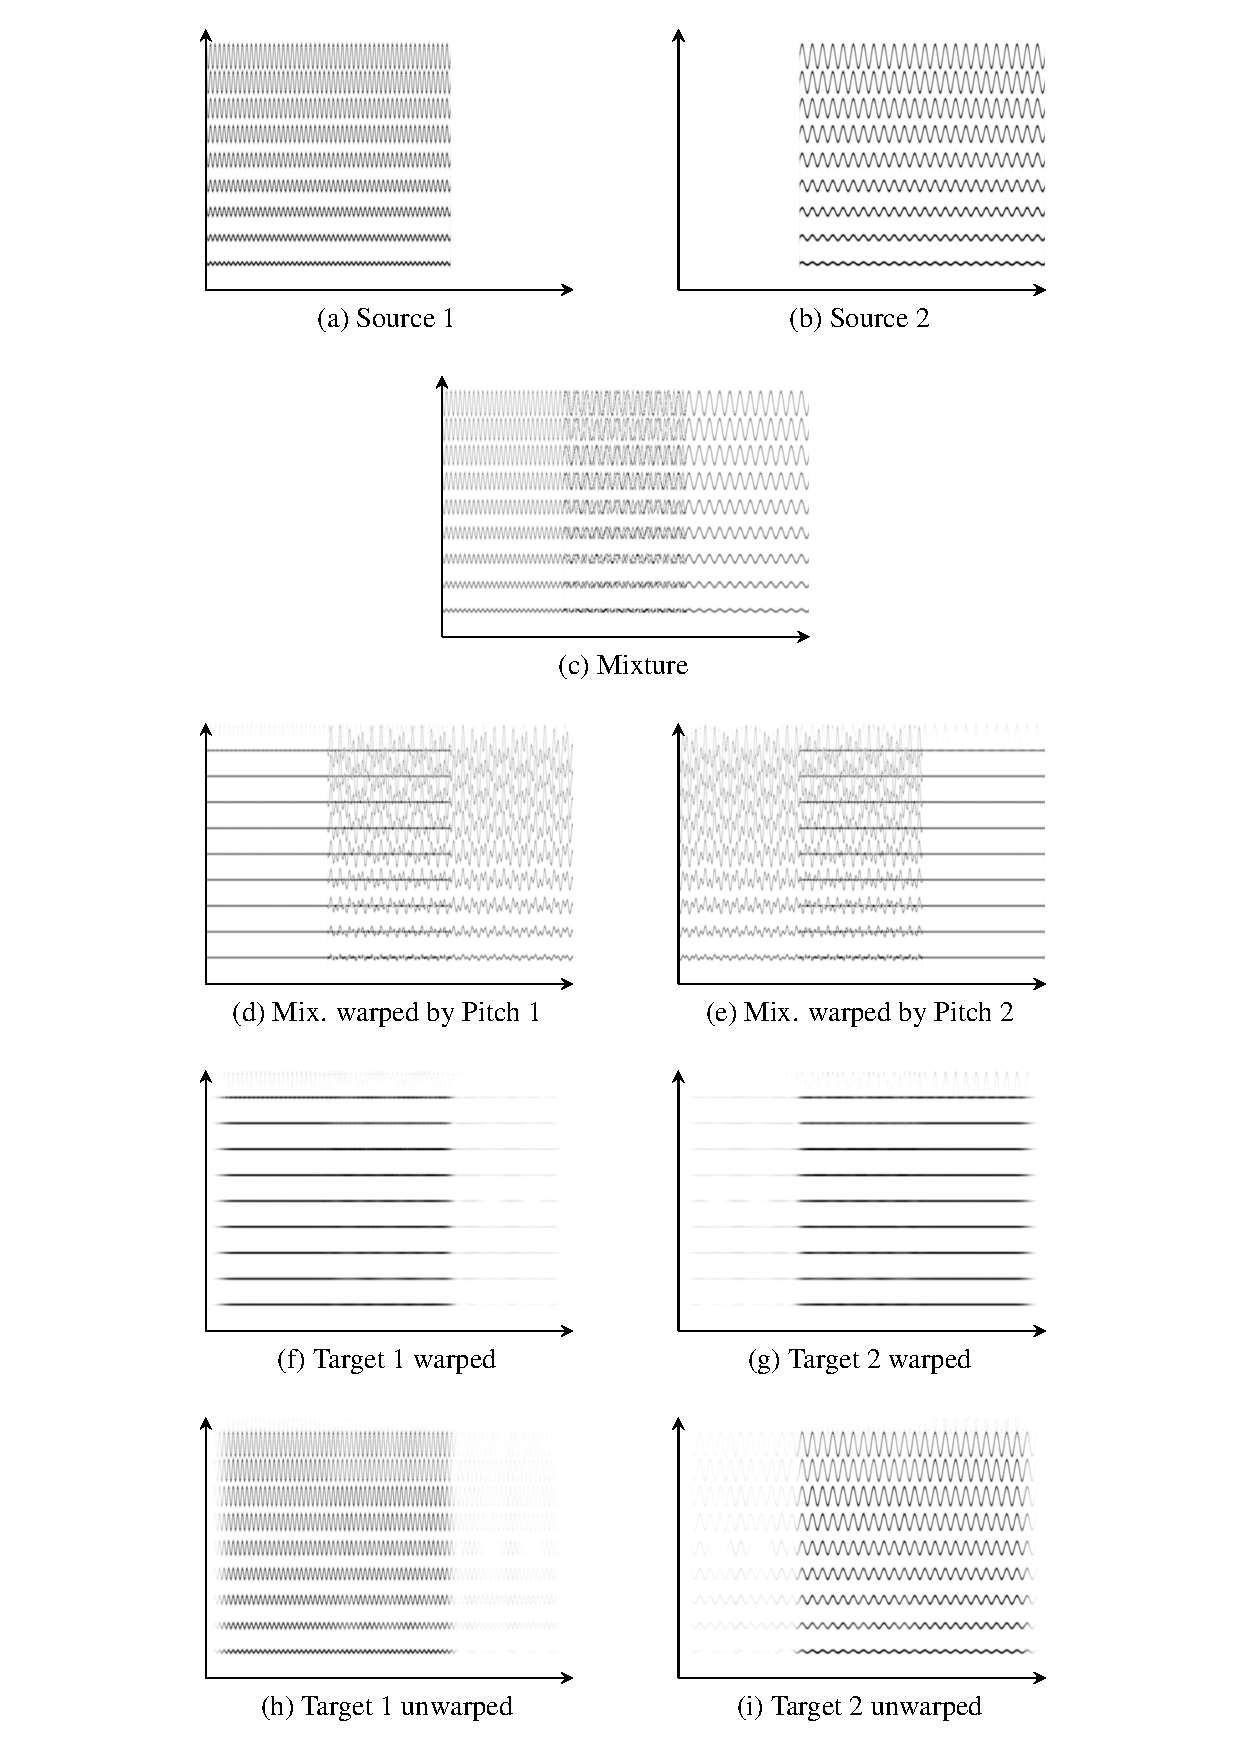
\includegraphics[width=\textwidth]{Chapters/05_Separation_Known/figures/toy.pdf}
\caption{Example of F0 variation informed NMF in the warped domain. \textit{Time} is shown on horizontal axes. \textit{Frequency} is shown on vertical axes.}%
\label{fig:warpingdemo}
\end{figure}

\section{Extending F0 Variation Informed Separation}

\marginpar{This results of this extension were submitted and evaluated in SiSEC 2015 and SiSEC 2016.}

In the previous section, we showed the effectiveness of a F0 variation informed separation system on our constrained unison source separation scenario.
In the following section I show how the method can be extended to the scenario of separating the vocals/lead from the accompaniment in professionally produced music.

% from zafar
Hereby I make use of one particularity of harmonic lead sources like singing voice.
It is their ability to produce vibration using vocal folds, further filtered by the vocal tract.
As a consequence, sung melodies are \textit{mostly} harmonic and therefore have a fundamental frequency.
If one can track the pitch of the vocals, one can then estimate the energy at the harmonics of the fundamental frequency and reconstruct the voice.

Such method is summarized in Figure~\ref{fig:methods_harmonicity}.
In a first step, the objective is to get estimates of the time-varying fundamental frequency for the lead at each time frame.
This can done by a suitable pitch detection method like~\cite{decheveigne02}.
A second step then is respect is then to track this fundamental frequency over time, in other words, to find the best sequence of estimates, in order to identify the melody line.
Such algorithms typically assume that the lead corresponds to the harmonic signal with strongest amplitude.
In this extension, I want show how the F0 variation informed separation system can be used in combination with a predominant melody estimation algorithm to extract singing voice from music.
\par
In a first step, the ``Melodia'' algorithm~\cite{salamon12} is used to obtain an estimate of the predominant melody from the mixture.
The mixture is then time warped based on the fundamental frequency of the melody so that it’s predominant solo part is nearly constant in F0. (See~\cite{salamon12} for details). The extraction is then carried out in time domain using efficient comb filtering.

\begin{figure}[htbp]
	\centering
  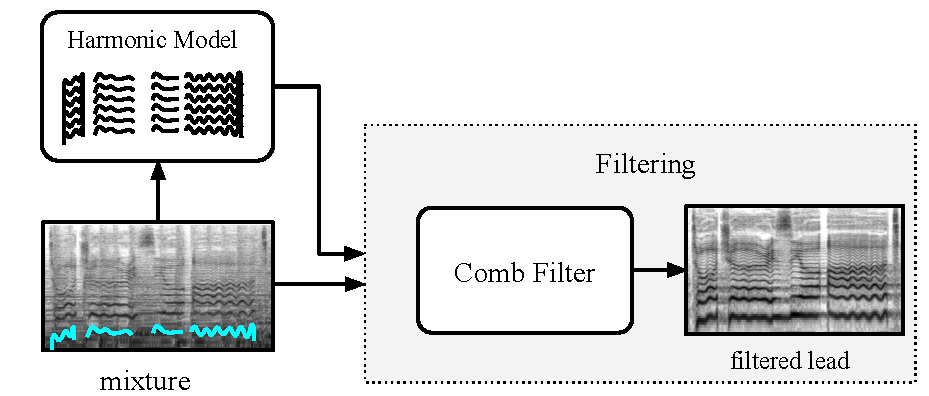
\includegraphics[width=\columnwidth]{Chapters/05_Separation_Known/figures/comb_filter.pdf}
	\caption{Block scheme diagram of a \textit{harmonic assumption} for vocals. In a first analysis step, the fundamental frequency of the lead signal is extracted. From it, a separation is obtained by filtering the mixture.}
	\label{fig:methods_harmonicity}
\end{figure}

\subsection{Predominant Melody Estimation}

The first step to extend the F0 variation informed separation system is to obtain a warp contour that follows the predominant source by means of extraction from the mixture (blind) or by human annotation (informed).
In the following I want to focus how to obtain such a warp contour using a predominant melody algorithm.\par

Estimating the fundamental frequency of one single source from a mixture of several sources is considered very difficult~\cite{klapuri08}.
However, in the case of vocal/accompaniment separation, we only consider one single source is considered as the lead source - usually the vocals.
This assumption often is applicable in modern popular music where such a lead source often is mixed louder than the other sources in the mix.
\par
Now, extracting the lead pitch contour is actually an ongoing field of research named ``melody estimation''.
However, compared to pitch or fundamental frequency, the term ``melody'' line  is only loosely defined.
A widely used definition is the one from Poliner et al. in~\cite{poliner07}:

\begin{quote}
  ``...melody is the single (monophonic) pitch sequence that a listener might reproduce if asked to whistle or hum a piece of polyphonic music, and that a listener would recognize as being the `essence` of that music when heard in comparison.''
\end{quote}

For a more comprehensive overview of melody extraction methods, the reader is referred to~\cite{salamon14}.
In this work, I follow the ``Understanding without Separation'' paradigm, which is seen as an advantage of a melody extraction method without applying a source separation system first (also see Chapter 1, Section 1.4.5~\cite{salamon14}).\par

In turn I used the \emph{Melodia} algorithm, published by Salamon et al. in 2012~\cite{salamon12} as the basis to extract vocals from the mixture.\par

\emph{Melodia} consists of four parts:
\noindent\textbf{1)}: a time-frequency transformation is applied and spectral peaks are extracted.
\textbf{2)}: these form the basis of a \emph{saliency} spectrogram that is computed using a weighted sum over all frequencies. This allows emphasize the predominant/salient frequencies in the signal and is the core part of the \emph{Melodia} algorithm.
\textbf{3)}: From the saliency map, again, peaks are extracted and then connected to a melody line. This would already a good starting point for the melody estimate but usually contains way to many outliers due to the noisiness of the saliency representation.
\textbf{4)}: The melody line is post-processed using a Viterbi decoder.
The purpose of it is to filter the contour by removing outliers, octave jumps and generally improves the smoothness of the contour using a number of heuristics.
It is important to note that this step is tracking the melody line of the previous step over time.
Usually this step is sensitive to the overall length of the processed mixture and often, this step is computed in a semantically meaningful segment of the mixture like a full track or a refrain.
\par
I applied the \emph{Melodia} using the implementation in Essentia~\cite{bogdanov13} with the default parameters (sample rate 22050 Hz, hop size = 3 ms, window size=46 ms).

\subsection{Source Extraction using Time Warping}

Once the predominant melody is obtained, the warp contour can be computed in the same way as described in Section~\ref{sub:time_warping} above.
In the unison scenario, however, we were globally warping the signal using a continuous warp contour.
In the case of full length tracks many parts are unvoiced and apply time warping on these segments would degrade the separation quality.
Therefore I only applied the warping on voiced parts and leave the non-vocal parts unaltered.
In order to do this, I used the built-in voice activity detection from \emph{Melodia}.
For all continuously voiced segments, I compute the warp contour from the  melody segments.
To reduce the complexity of the extraction, compared to the NMF mentioned in Section~\ref{sub:frequency_modulation}, I designed a comb filter that can extract the voice in the warped time domain.
Therefore I used a simple IIR Filter with the frequency response

\begin{equation}
  H(z) = \frac{1}{1 - 0.75^z{-P}},
\end{equation}

where \(P\) is constant --- due to the time warping --- pitch period in samples.
In order to then extract the vocals, zero-phase filtering is applied.
The extracted vocals were inverse warped to linear time and the accompaniment signal is created by subtracting the estimated vocals from the mixture signals.
Each excerpt is then linearly crossfaded into the unaltered, accompaniment/mixture using a 10ms window.
To further reduce the complexity of the separation system, instead one comb filter for each excerpts, I modified the warping algorithm so that a user defined target pitch \(P\), rounded to integer, is used.
That way, the full signal is inverse warped and resampled to the same pitch, which then only requires a single comb filter to extract the signal.
A stereo signal is produced by using a signal filtering both channels individually.

The full procedure is depicted in Figure~\ref{fig:warp_sisec_demo}.

\begin{figure}
\begin{tabular}{cc}
  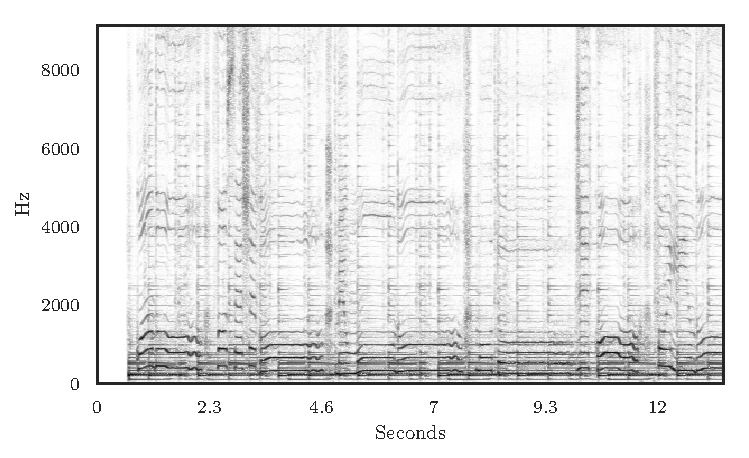
\includegraphics[width=65mm]{Chapters/05_Separation_Known/warp-demo/Mixture.pdf} & 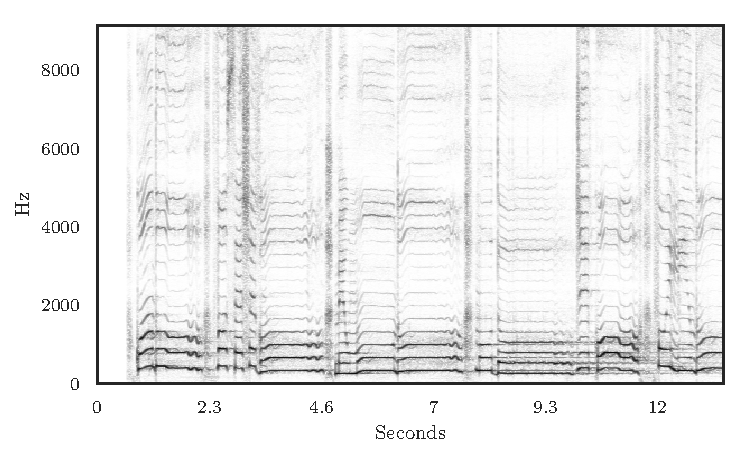
\includegraphics[width=65mm]{Chapters/05_Separation_Known/warp-demo/reference.pdf} \\
(a) Mixture Magnitude STFT & (b) Ground Truth Vocals \\[6pt]
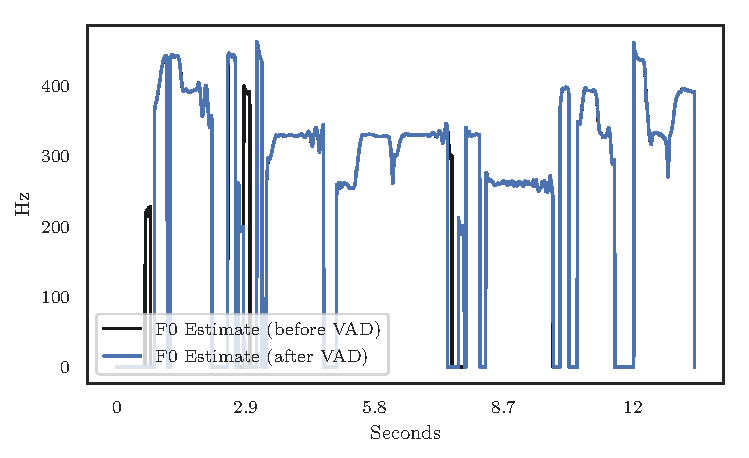
\includegraphics[width=65mm]{Chapters/05_Separation_Known/warp-demo/Melodia.pdf} & 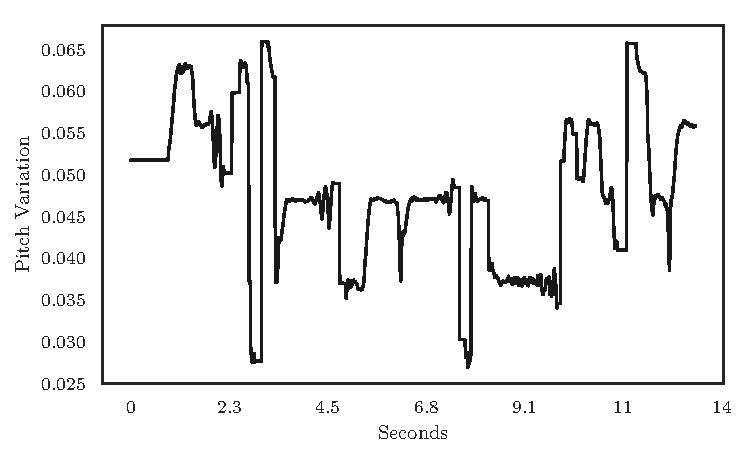
\includegraphics[width=65mm]{Chapters/05_Separation_Known/warp-demo/Contour.pdf} \\
(c) Melody Estimate & (d) Warp Contour \\[6pt]
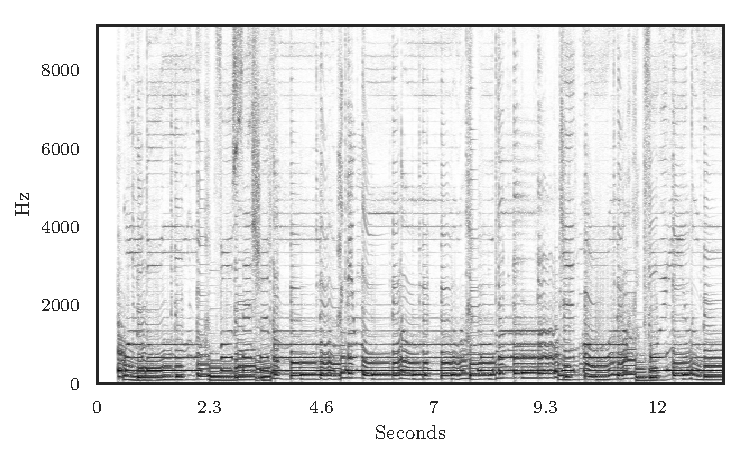
\includegraphics[width=65mm]{Chapters/05_Separation_Known/warp-demo/warped.pdf} & 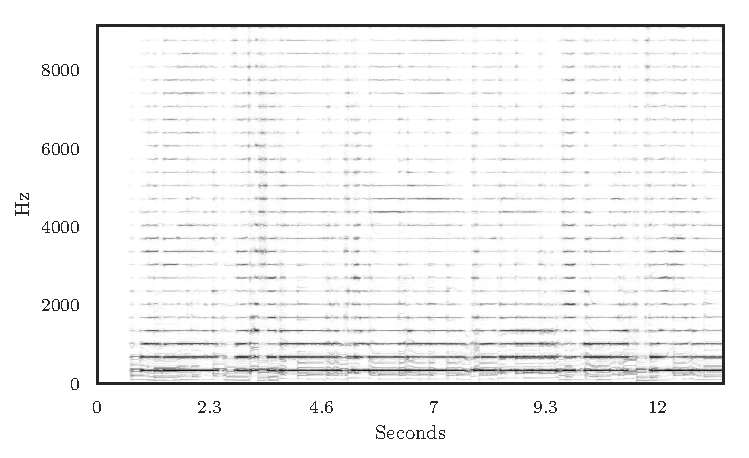
\includegraphics[width=65mm]{Chapters/05_Separation_Known/warp-demo/warped_filtered.pdf} \\
(e) Warped Mixture & (f) Filtered Mixture \\[6pt]
\multicolumn{2}{c}{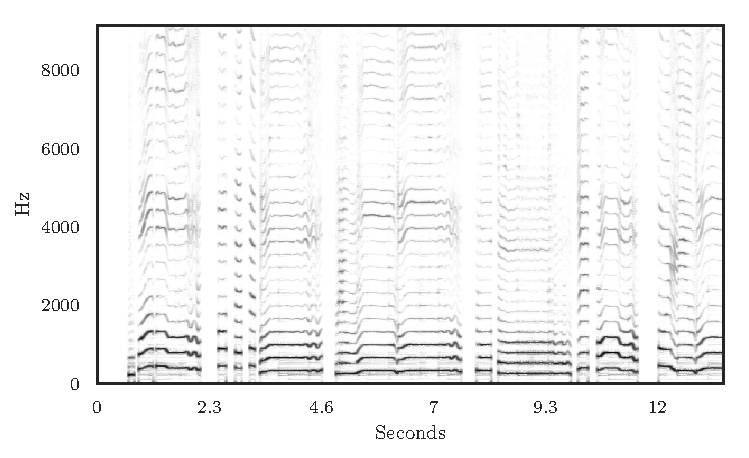
\includegraphics[width=65mm]{Chapters/05_Separation_Known/warp-demo/Estimate.pdf} }\\
\multicolumn{2}{c}{(g) Vocals Estimate}
\end{tabular}
\caption{Examples of a F0 variation informed separation of the audio track \emph{Tamy - Que Pena Tanto Fa} form the (MASS) dataset~\cite{MTGMASSdb}.}%
\label{fig:warp_sisec_demo}
\end{figure}

\subsection{Results on SiSEC 2015}
\label{ssec:performance_sisec15}

The algorithm has been applied to the Mixing Secret Dataset 100 (MSD100) dataset,  consisting of a total of 100 songs of different styles.
The separation results were evaluated using BSSeval~\cite{fevotte05} and submitted to the SiSEC 2015 evaluation challenge~\cite{ono15}.
The system was ranked in the last third of the participants and scored only slightly better than RPCA based methods~\cite{huang12}.
The reason for this is that our proposed system highly depends on the melody estimation algorithm which in turns is based on the assumption that there exist a predominant melody in the mixture.
Unfortunately, the newly created MSD100 dataset was not mixed using professional mastering, resulting in vocals that are below average in loudness.
Due to the small energy, they were not detected as voiced by \emph{Melodia}, hence the warping was either not applied. Even worse, sometimes the pitch estimates were one octave off producing severe artifacts due to extreme warping.\par
On the positive side, the proposed method is of very low complexity and generally implemented in Python and has very low computational complexity.

\subsection{Improving Voiced/Unvoiced Detection using Deep Neural Networks}

As mentioned in the previous section, voice activity detection is of paramount importance in the proposed music separation system.
Therefore, I decided to evaluate if the performance of the system can be improved by using a more robust voice activity detection method as a separate preprocessing step.
\par
Shortly after I submitted the separation results to the SiSEC 2015 evaluation campaign, the whole audio community was shaken up by the recent success of deep learning throughout several audio related tasks that go beyond automatic speech recognition.
Among them are several tasks related to music information retrieval (MIR) such as singing voice detection which received major breakthroughs in 2014 and 2015~\cite{lehner14, lehner15, Leglaive15, schlueter15}.
\par
Locking back, at that time, I did not have enough knowledge to understand how and why deep learning method are so successful~\footnote{And even today, very few people would say that the deep learning community made significant progress regarding the understanding of DNNs.}.
Therefore, I decided to deploy a state-of-the-art singing voice detection system into my separation pipeline and evaluate just the end-to-end performance.
I chose to reimplement the system by Leglaive~\cite{Leglaive15}, since it was a good compromise between complexity (its uses hand-crafted features instead of large STFT frames) and performance.
In fact, the system reached a state-of-the-art accuracy of 91.5\% (F-measure of 91.5) for classifying frames of singing voice for the annotated \emph{Jamendo} singing voice detection dataset~\cite{ramona08}, which is an improvement of more than 10\% compared to the best performing non-DNN system.
I want to briefly describe the system published in in~\cite{Leglaive15}, for more details, the reader is referred to the original authors publications.
Also in the course of this thesis, more of my work is based on the deep learning framework and will be explained in further details in Chapter~\ref{cha:countnet}.
\par
The method proposed in~\cite{Leglaive15} is based on a recurrent neural network (RNN) layer is very similar to a classical fully connected neural network, except that RNN applies the same set of weights recursively over an input sequence.
RNNs excel at detecting structure in sequential data of arbitrary length.
This makes it ideal to model time series, however, in practice, the temporal context learnt is limited to only a few time instances, because of the vanishing gradient problem~\cite{Hochreiter98}.
To alleviate this problem, forgetting factors (also called gating) were proposed.
One of the most popular gated recurrent cells is the Long Short-Term Memory (LSTM)~\cite{Hochreiter97} cell.
Its effectiveness has been proven in various applications and LSTMs are the state-of-the-art approach for speech recognition~\cite{Graves13}.
The basic structure of such a sequential network is depicted in Figure~\ref{fig:lstm_2}.
\begin{figure}
  \centering
  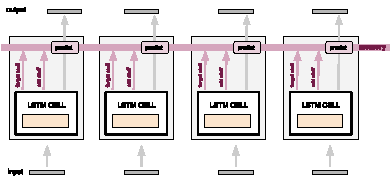
\includegraphics[width=0.8\textwidth]{Chapters/05_Separation_Known/figures/lstm_2.pdf}
  \caption{Simpliefied Block diagram of a Long Short-Term Memory Network.}
  \label{fig:lstm_2}
\end{figure}
The input of the network is a 80 dimensional feature vector consisting of harmonically and percussively enhanced STFT frames of the mixture as described in~\cite{ono08}.
The output of the network is a framewise integer, indicating `1.0` for singing voice and `0.0` for \emph{unvoiced} frames.
I trained the network using a fixed number of frames from the DSD100 training dataset.
The vocal activity labels were obtained from the dataset by analyzing the true vocals.
The network was created and trained using the Keras python framework~\cite{chollet15}.
I stacked up to three layers using the parameters as mentioned in~\cite{Leglaive15} but used unidirectional LSTMs instead of bi-directional to reduce computation complexity.
The trained network achieves an accuracy of 85\% on the separate test set.\par
While the original network proposed in~\cite{Leglaive15} was framed as  classification problem, I modified the sigmoid output activation and replaced it with a linear activation to get a linear gain \(g\) instead of probability.
This gain is then multiplied with the mixture signal so that segments with less energy are reduced in volume.
In experiments I found out that this helps the \emph{Melodia} algorithm to better detect vocal activity throughout an audio track and therefore yields in melody estimates with fewer errors.

\begin{figure}
  \centering
  % This file was created by matlab2tikz.
%
%The latest updates can be retrieved from
%  http://www.mathworks.com/matlabcentral/fileexchange/22022-matlab2tikz-matlab2tikz
%where you can also make suggestions and rate matlab2tikz.
%
\begin{tikzpicture}

\begin{axis}[%
width=1.396in,
height=0.78in,
at={(0.57in,3.0in)},
scale only axis,
xmin=0.5,
xmax=2.5,
ymin=-11.8456832139538,
ymax=12.0983588349663,
ylabel style={font=\color{white!15!black}},
ylabel={SDR},
axis background/.style={fill=white},
xticklabels={},
title style={font=\bfseries},
title={vocals},
ymajorgrids,
yminorgrids
]
\addplot [color=black, forget plot]
  table[row sep=crcr]{%
0.6	-1.9758567749213\\
0.6	-1.1472747974891\\
0.6	0.0481517271656759\\
1.4	0.0481517271656759\\
1.4	-1.1472747974891\\
1.4	-1.9758567749213\\
1.4	-2.8044387523535\\
1.4	-3.6836695149443\\
0.6	-3.6836695149443\\
0.6	-2.8044387523535\\
0.6	-1.9758567749213\\
};
\addplot [color=black, forget plot]
  table[row sep=crcr]{%
1.6	-0.507353682851228\\
1.6	0.113338890967634\\
1.6	0.852771078194694\\
2.4	0.852771078194694\\
2.4	0.113338890967634\\
2.4	-0.507353682851228\\
2.4	-1.12804625667009\\
2.4	-1.94274438664256\\
1.6	-1.94274438664256\\
1.6	-1.12804625667009\\
1.6	-0.507353682851228\\
};
\addplot [color=black, forget plot]
  table[row sep=crcr]{%
1	-6.78225690045683\\
1	-3.6836695149443\\
};
\addplot [color=black, forget plot]
  table[row sep=crcr]{%
2	-4.92374070693745\\
2	-1.94274438664256\\
};
\addplot [color=black, forget plot]
  table[row sep=crcr]{%
1	2.55938991049521\\
1	0.0481517271656759\\
};
\addplot [color=black, forget plot]
  table[row sep=crcr]{%
2	2.42428921907715\\
2	0.852771078194694\\
};
\addplot [color=black, forget plot]
  table[row sep=crcr]{%
0.95	-6.78225690045683\\
1.05	-6.78225690045683\\
};
\addplot [color=black, forget plot]
  table[row sep=crcr]{%
1.95	-4.92374070693745\\
2.05	-4.92374070693745\\
};
\addplot [color=black, forget plot]
  table[row sep=crcr]{%
0.95	2.55938991049521\\
1.05	2.55938991049521\\
};
\addplot [color=black, forget plot]
  table[row sep=crcr]{%
1.95	2.42428921907715\\
2.05	2.42428921907715\\
};
\addplot [color=CTlink, forget plot]
  table[row sep=crcr]{%
0.6	-1.9758567749213\\
1.4	-1.9758567749213\\
};
\addplot [color=CTlink, forget plot]
  table[row sep=crcr]{%
1.6	-0.507353682851228\\
2.4	-0.507353682851228\\
};
\addplot [color=CTlink, draw=none, mark=+, mark options={solid, CTlink}, forget plot]
  table[row sep=crcr]{%
1	-14.3959348646932\\
1	-9.54992631980009\\
2	-8.26993351147881\\
};
\addplot [color=CTlink, draw=none, mark=o, mark options={solid, CTlink}, forget plot]
  table[row sep=crcr]{%
2	-11.9927544705679\\
};
\node[above, align=center, font=\color{CTlink}]
at (axis cs:1.25,0.058) {-2.0};
\node[above, align=center, font=\color{CTlink}]
at (axis cs:2.25,0.858) {-0.5};
\end{axis}

\begin{axis}[%
width=1.396in,
height=0.78in,
at={(0.57in,2in)},
scale only axis,
xmin=0.5,
xmax=2.5,
ymin=-3.96838110928441,
ymax=33.8051471982415,
ylabel style={font=\color{white!15!black}},
ylabel={ISR},
axis background/.style={fill=white},
title style={font=\bfseries},
xticklabels={},
xmajorgrids,
xminorgrids,
ymajorgrids,
yminorgrids
]
\addplot [color=black, forget plot]
  table[row sep=crcr]{%
0.6	3.50620881354056\\
0.6	4.05770869257335\\
0.6	4.44397637616963\\
1.4	4.44397637616963\\
1.4	4.05770869257335\\
1.4	3.50620881354056\\
1.4	2.95470893450776\\
1.4	1.96009545714002\\
0.6	1.96009545714002\\
0.6	2.95470893450776\\
0.6	3.50620881354056\\
};
\addplot [color=black, forget plot]
  table[row sep=crcr]{%
1.6	2.14304180047585\\
1.6	2.51961815215558\\
1.6	2.90572551289987\\
2.4	2.90572551289987\\
2.4	2.51961815215558\\
2.4	2.14304180047585\\
2.4	1.76646544879613\\
2.4	1.20967651986024\\
1.6	1.20967651986024\\
1.6	1.76646544879613\\
1.6	2.14304180047585\\
};
\addplot [color=black, forget plot]
  table[row sep=crcr]{%
1	-0.40174698709892\\
1	1.96009545714002\\
};
\addplot [color=black, forget plot]
  table[row sep=crcr]{%
2	-0.482277241947297\\
2	1.20967651986024\\
};
\addplot [color=black, forget plot]
  table[row sep=crcr]{%
1	7.91643810164209\\
1	4.44397637616963\\
};
\addplot [color=black, forget plot]
  table[row sep=crcr]{%
2	4.97064159442628\\
2	2.90572551289987\\
};
\addplot [color=black, forget plot]
  table[row sep=crcr]{%
0.95	-0.40174698709892\\
1.05	-0.40174698709892\\
};
\addplot [color=black, forget plot]
  table[row sep=crcr]{%
1.95	-0.482277241947297\\
2.05	-0.482277241947297\\
};
\addplot [color=black, forget plot]
  table[row sep=crcr]{%
0.95	7.91643810164209\\
1.05	7.91643810164209\\
};
\addplot [color=black, forget plot]
  table[row sep=crcr]{%
1.95	4.97064159442628\\
2.05	4.97064159442628\\
};
\addplot [color=CTlink, forget plot]
  table[row sep=crcr]{%
0.6	3.50620881354056\\
1.4	3.50620881354056\\
};
\addplot [color=CTlink, forget plot]
  table[row sep=crcr]{%
1.6	2.14304180047585\\
2.4	2.14304180047585\\
};
\addplot [color=CTlink, draw=none, mark=+, mark options={solid, CTlink}, forget plot]
  table[row sep=crcr]{%
1	-3.28408406277023\\
2	6.397293668273\\
2	7.20875679699654\\
2	-2.83798717487847\\
};
\node[above, align=center, font=\color{CTlink}]
at (axis cs:1.25,4.47) {3.5};
\node[above, align=center, font=\color{CTlink}]
at (axis cs:2.25,2.959) {2.1};
\end{axis}

\begin{axis}[%
width=1.396in,
height=0.78in,
at={(0.57in,1in)},
scale only axis,
xmin=0.5,
xmax=2.5,
ymin=-24.6956290240449,
ymax=20.9072423316779,
ylabel style={font=\color{white!15!black}},
ylabel={SIR},
axis background/.style={fill=white},
title style={font=\bfseries},
xticklabels={},
xmajorgrids,
xminorgrids,
ymajorgrids,
yminorgrids
]
\addplot [color=black, forget plot]
  table[row sep=crcr]{%
0.6	-2.48453261782208\\
0.6	-0.3132784539727\\
0.6	2.53580554448196\\
1.4	2.53580554448196\\
1.4	-0.3132784539727\\
1.4	-2.48453261782208\\
1.4	-4.65578678167146\\
1.4	-7.24322976085196\\
0.6	-7.24322976085196\\
0.6	-4.65578678167146\\
0.6	-2.48453261782208\\
};
\addplot [color=black, forget plot]
  table[row sep=crcr]{%
1.6	-2.48758804804584\\
1.6	-0.324985030085506\\
1.6	2.51267739901011\\
2.4	2.51267739901011\\
2.4	-0.324985030085506\\
2.4	-2.48758804804584\\
2.4	-4.65019106600618\\
2.4	-7.22739431445643\\
1.6	-7.22739431445643\\
1.6	-4.65019106600618\\
1.6	-2.48758804804584\\
};
\addplot [color=black, forget plot]
  table[row sep=crcr]{%
1	-20.2011258746078\\
1	-7.24322976085196\\
};
\addplot [color=black, forget plot]
  table[row sep=crcr]{%
2	-18.5324438120827\\
2	-7.22739431445643\\
};
\addplot [color=black, forget plot]
  table[row sep=crcr]{%
1	13.5361423309813\\
1	2.53580554448196\\
};
\addplot [color=black, forget plot]
  table[row sep=crcr]{%
2	12.314299783158\\
2	2.51267739901011\\
};
\addplot [color=black, forget plot]
  table[row sep=crcr]{%
0.95	-20.2011258746078\\
1.05	-20.2011258746078\\
};
\addplot [color=black, forget plot]
  table[row sep=crcr]{%
1.95	-18.5324438120827\\
2.05	-18.5324438120827\\
};
\addplot [color=black, forget plot]
  table[row sep=crcr]{%
0.95	13.5361423309813\\
1.05	13.5361423309813\\
};
\addplot [color=black, forget plot]
  table[row sep=crcr]{%
1.95	12.314299783158\\
2.05	12.314299783158\\
};
\addplot [color=CTlink, forget plot]
  table[row sep=crcr]{%
0.6	-2.48453261782208\\
1.4	-2.48453261782208\\
};
\addplot [color=CTlink, forget plot]
  table[row sep=crcr]{%
1.6	-2.48758804804584\\
2.4	-2.48758804804584\\
};
\node[above, align=center, font=\color{CTlink}]
at (axis cs:1.25,2.587) {-2.5};
\node[above, align=center, font=\color{CTlink}]
at (axis cs:2.25,2.528) {-2.5};
\end{axis}

\begin{axis}[%
width=1.396in,
height=0.78in,
at={(0.57in,0.0in)},
scale only axis,
xmin=0.5,
xmax=2.5,
ymin=-9.33793882104533,
ymax=19.711869659802,
ylabel style={font=\color{white!15!black}},
ylabel={SAR},
axis background/.style={fill=white},
title style={font=\bfseries},
xticklabels={},
extra x ticks={1, 2},
extra x tick labels={STO, STOD},
xmajorgrids,
xminorgrids,
ymajorgrids,
yminorgrids
]
\addplot [color=black, forget plot]
  table[row sep=crcr]{%
0.6	-1.49008262500965\\
0.6	-0.937140481566175\\
0.6	-0.397036079394241\\
1.4	-0.397036079394241\\
1.4	-0.937140481566175\\
1.4	-1.49008262500965\\
1.4	-2.04302476845313\\
1.4	-2.88741276240511\\
0.6	-2.88741276240511\\
0.6	-2.04302476845313\\
0.6	-1.49008262500965\\
};
\addplot [color=black, forget plot]
  table[row sep=crcr]{%
1.6	-1.92712180362399\\
1.6	-1.51401965317932\\
1.6	-1.28308624281028\\
2.4	-1.28308624281028\\
2.4	-1.51401965317932\\
2.4	-1.92712180362399\\
2.4	-2.34022395406866\\
2.4	-3.14364249696425\\
1.6	-3.14364249696425\\
1.6	-2.34022395406866\\
1.6	-1.92712180362399\\
};
\addplot [color=black, forget plot]
  table[row sep=crcr]{%
1	-6.47916647615166\\
1	-2.88741276240511\\
};
\addplot [color=black, forget plot]
  table[row sep=crcr]{%
2	-5.90482132380423\\
2	-3.14364249696425\\
};
\addplot [color=black, forget plot]
  table[row sep=crcr]{%
1	2.22561651276376\\
1	-0.397036079394241\\
};
\addplot [color=black, forget plot]
  table[row sep=crcr]{%
2	0.754545016067411\\
2	-1.28308624281028\\
};
\addplot [color=black, forget plot]
  table[row sep=crcr]{%
0.95	-6.47916647615166\\
1.05	-6.47916647615166\\
};
\addplot [color=black, forget plot]
  table[row sep=crcr]{%
1.95	-5.90482132380423\\
2.05	-5.90482132380423\\
};
\addplot [color=black, forget plot]
  table[row sep=crcr]{%
0.95	2.22561651276376\\
1.05	2.22561651276376\\
};
\addplot [color=black, forget plot]
  table[row sep=crcr]{%
1.95	0.754545016067411\\
2.05	0.754545016067411\\
};
\addplot [color=CTlink, forget plot]
  table[row sep=crcr]{%
0.6	-1.49008262500965\\
1.4	-1.49008262500965\\
};
\addplot [color=CTlink, forget plot]
  table[row sep=crcr]{%
1.6	-1.92712180362399\\
2.4	-1.92712180362399\\
};
\addplot [color=CTlink, draw=none, mark=+, mark options={solid, CTlink}, forget plot]
  table[row sep=crcr]{%
1	6.98498144484663\\
2	-7.11676805264549\\
2	-6.06944522075845\\
2	1.8857615511021\\
2	-6.78832410475883\\
2	3.48218878687135\\
};
\node[above, align=center, font=\color{CTlink}]
at (axis cs:1.25,-0.373) {-1.5};
\node[above, align=center, font=\color{CTlink}]
at (axis cs:2.25,-1.272) {-1.9};
\end{axis}

\begin{axis}[%
width=1.396in,
height=0.78in,
at={(2.571in,3in)},
scale only axis,
xmin=0.5,
xmax=2.5,
ymin=-11.8456832139538,
ymax=12.0983588349663,
ylabel style={font=\color{white!15!black}},
ylabel={SDR},
axis background/.style={fill=white},
title style={font=\bfseries},
title={accompaniment},
xticklabels={},
xmajorgrids,
xminorgrids,
ymajorgrids,
yminorgrids
]
\addplot [color=black, forget plot]
  table[row sep=crcr]{%
0.6	4.07993386412816\\
0.6	4.5571974306502\\
0.6	5.62931832744247\\
1.4	5.62931832744247\\
1.4	4.5571974306502\\
1.4	4.07993386412816\\
1.4	3.60267029760612\\
1.4	3.4797877267991\\
0.6	3.4797877267991\\
0.6	3.60267029760612\\
0.6	4.07993386412816\\
};
\addplot [color=black, forget plot]
  table[row sep=crcr]{%
1.6	5.71965452157484\\
1.6	6.33294034116551\\
1.6	7.02863101460487\\
2.4	7.02863101460487\\
2.4	6.33294034116551\\
2.4	5.71965452157484\\
2.4	5.10636870198416\\
2.4	4.26647456977611\\
1.6	4.26647456977611\\
1.6	5.10636870198416\\
1.6	5.71965452157484\\
};
\addplot [color=black, forget plot]
  table[row sep=crcr]{%
1	0.944593194955716\\
1	3.4797877267991\\
};
\addplot [color=black, forget plot]
  table[row sep=crcr]{%
2	2.47249259717672\\
2	4.26647456977611\\
};
\addplot [color=black, forget plot]
  table[row sep=crcr]{%
1	7.86830964455784\\
1	5.62931832744247\\
};
\addplot [color=black, forget plot]
  table[row sep=crcr]{%
2	9.53990054010412\\
2	7.02863101460487\\
};
\addplot [color=black, forget plot]
  table[row sep=crcr]{%
0.95	0.944593194955716\\
1.05	0.944593194955716\\
};
\addplot [color=black, forget plot]
  table[row sep=crcr]{%
1.95	2.47249259717672\\
2.05	2.47249259717672\\
};
\addplot [color=black, forget plot]
  table[row sep=crcr]{%
0.95	7.86830964455784\\
1.05	7.86830964455784\\
};
\addplot [color=black, forget plot]
  table[row sep=crcr]{%
1.95	9.53990054010412\\
2.05	9.53990054010412\\
};
\addplot [color=CTlink, forget plot]
  table[row sep=crcr]{%
0.6	4.07993386412816\\
1.4	4.07993386412816\\
};
\addplot [color=CTlink, forget plot]
  table[row sep=crcr]{%
1.6	5.71965452157484\\
2.4	5.71965452157484\\
};
\addplot [color=CTlink, draw=none, mark=+, mark options={solid, CTlink}, forget plot]
  table[row sep=crcr]{%
2	11.2995823151338\\
};
\node[above, align=center, font=\color{CTlink}]
at (axis cs:1.25,5.689) {4.1};
\node[above, align=center, font=\color{CTlink}]
at (axis cs:2.25,7.072) {5.7};
\end{axis}

\begin{axis}[%
width=1.396in,
height=0.78in,
at={(2.571in,2in)},
scale only axis,
xmin=0.5,
xmax=2.5,
ymin=-3.96838110928441,
ymax=33.8051471982415,
ylabel style={font=\color{white!15!black}},
ylabel={ISR},
axis background/.style={fill=white},
title style={font=\bfseries},
xticklabels={},
xmajorgrids,
xminorgrids,
ymajorgrids,
yminorgrids
]
\addplot [color=black, forget plot]
  table[row sep=crcr]{%
0.6	14.1846658645635\\
0.6	14.9939408596737\\
0.6	15.6697782504659\\
1.4	15.6697782504659\\
1.4	14.9939408596737\\
1.4	14.1846658645635\\
1.4	13.3753908694533\\
1.4	12.0249130473631\\
0.6	12.0249130473631\\
0.6	13.3753908694533\\
0.6	14.1846658645635\\
};
\addplot [color=black, forget plot]
  table[row sep=crcr]{%
1.6	18.0632858964916\\
1.6	19.2169237215004\\
1.6	20.2624022975336\\
2.4	20.2624022975336\\
2.4	19.2169237215004\\
2.4	18.0632858964916\\
2.4	16.9096480714828\\
2.4	15.066573449782\\
1.6	15.066573449782\\
1.6	16.9096480714828\\
1.6	18.0632858964916\\
};
\addplot [color=black, forget plot]
  table[row sep=crcr]{%
1	7.41703006231415\\
1	12.0249130473631\\
};
\addplot [color=black, forget plot]
  table[row sep=crcr]{%
2	10.6448624248896\\
2	15.066573449782\\
};
\addplot [color=black, forget plot]
  table[row sep=crcr]{%
1	19.4650732883217\\
1	15.6697782504659\\
};
\addplot [color=black, forget plot]
  table[row sep=crcr]{%
2	27.7268965181242\\
2	20.2624022975336\\
};
\addplot [color=black, forget plot]
  table[row sep=crcr]{%
0.95	7.41703006231415\\
1.05	7.41703006231415\\
};
\addplot [color=black, forget plot]
  table[row sep=crcr]{%
1.95	10.6448624248896\\
2.05	10.6448624248896\\
};
\addplot [color=black, forget plot]
  table[row sep=crcr]{%
0.95	19.4650732883217\\
1.05	19.4650732883217\\
};
\addplot [color=black, forget plot]
  table[row sep=crcr]{%
1.95	27.7268965181242\\
2.05	27.7268965181242\\
};
\addplot [color=CTlink, forget plot]
  table[row sep=crcr]{%
0.6	14.1846658645635\\
1.4	14.1846658645635\\
};
\addplot [color=CTlink, forget plot]
  table[row sep=crcr]{%
1.6	18.0632858964916\\
2.4	18.0632858964916\\
};
\addplot [color=CTlink, draw=none, mark=+, mark options={solid, CTlink}, forget plot]
  table[row sep=crcr]{%
1	21.401905071888\\
1	2.74498453261405\\
1	21.9336226665764\\
2	6.88346229505207\\
};
\node[above, align=center, font=\color{CTlink}]
at (axis cs:1.25,15.812) {14.2};
\node[above, align=center, font=\color{CTlink}]
at (axis cs:2.25,20.342) {18.1};
\end{axis}

\begin{axis}[%
width=1.396in,
height=0.78in,
at={(2.571in,1in)},
scale only axis,
xmin=0.5,
xmax=2.5,
ymin=-24.6956290240449,
ymax=20.9072423316779,
ylabel style={font=\color{white!15!black}},
ylabel={SIR},
axis background/.style={fill=white},
xticklabels={},
title style={font=\bfseries},
xmajorgrids,
xminorgrids,
ymajorgrids,
yminorgrids
]
\addplot [color=black, forget plot]
  table[row sep=crcr]{%
0.6	8.39513700131584\\
0.6	9.26439178676195\\
0.6	10.033272550563\\
1.4	10.033272550563\\
1.4	9.26439178676195\\
1.4	8.39513700131584\\
1.4	7.52588221586974\\
1.4	6.11826647815662\\
0.6	6.11826647815662\\
0.6	7.52588221586974\\
0.6	8.39513700131584\\
};
\addplot [color=black, forget plot]
  table[row sep=crcr]{%
1.6	7.54419258595698\\
1.6	8.4682930672431\\
1.6	9.60417638684285\\
2.4	9.60417638684285\\
2.4	8.4682930672431\\
2.4	7.54419258595698\\
2.4	6.62009210467087\\
2.4	5.44215271286093\\
1.6	5.44215271286093\\
1.6	6.62009210467087\\
1.6	7.54419258595698\\
};
\addplot [color=black, forget plot]
  table[row sep=crcr]{%
1	0.911564014698467\\
1	6.11826647815662\\
};
\addplot [color=black, forget plot]
  table[row sep=crcr]{%
2	3.09557012359525\\
2	5.44215271286093\\
};
\addplot [color=black, forget plot]
  table[row sep=crcr]{%
1	13.608095186407\\
1	10.033272550563\\
};
\addplot [color=black, forget plot]
  table[row sep=crcr]{%
2	13.8885853596125\\
2	9.60417638684285\\
};
\addplot [color=black, forget plot]
  table[row sep=crcr]{%
0.95	0.911564014698467\\
1.05	0.911564014698467\\
};
\addplot [color=black, forget plot]
  table[row sep=crcr]{%
1.95	3.09557012359525\\
2.05	3.09557012359525\\
};
\addplot [color=black, forget plot]
  table[row sep=crcr]{%
0.95	13.608095186407\\
1.05	13.608095186407\\
};
\addplot [color=black, forget plot]
  table[row sep=crcr]{%
1.95	13.8885853596125\\
2.05	13.8885853596125\\
};
\addplot [color=CTlink, forget plot]
  table[row sep=crcr]{%
0.6	8.39513700131584\\
1.4	8.39513700131584\\
};
\addplot [color=CTlink, forget plot]
  table[row sep=crcr]{%
1.6	7.54419258595698\\
2.4	7.54419258595698\\
};
\node[above, align=center, font=\color{CTlink}]
at (axis cs:1.25,10.06) {8.4};
\node[above, align=center, font=\color{CTlink}]
at (axis cs:2.25,9.614) {7.5};
\end{axis}

\begin{axis}[%
width=1.396in,
height=0.78in,
at={(2.571in,0in)},
scale only axis,
xmin=0.5,
xmax=2.5,
ymin=-9.33793882104533,
ymax=19.711869659802,
ylabel style={font=\color{white!15!black}},
ylabel={SAR},
axis background/.style={fill=white},
title style={font=\bfseries},
xticklabels={},
yticklabels={},
extra x ticks={1, 2},
extra x tick labels={STO, STOD},
xmajorgrids,
xminorgrids,
ymajorgrids,
yminorgrids
]
\addplot [color=black, forget plot]
  table[row sep=crcr]{%
0.6	6.88286322756687\\
0.6	7.33779171661827\\
0.6	7.88948907206887\\
1.4	7.88948907206887\\
1.4	7.33779171661827\\
1.4	6.88286322756687\\
1.4	6.42793473851547\\
1.4	5.84055264173005\\
0.6	5.84055264173005\\
0.6	6.42793473851547\\
0.6	6.88286322756687\\
};
\addplot [color=black, forget plot]
  table[row sep=crcr]{%
1.6	10.7036329091479\\
1.6	11.6159696204354\\
1.6	12.537223176303\\
2.4	12.537223176303\\
2.4	11.6159696204354\\
2.4	10.7036329091479\\
2.4	9.79129619786032\\
2.4	8.4281819325013\\
1.6	8.4281819325013\\
1.6	9.79129619786032\\
1.6	10.7036329091479\\
};
\addplot [color=black, forget plot]
  table[row sep=crcr]{%
1	3.31208622647544\\
1	5.84055264173005\\
};
\addplot [color=black, forget plot]
  table[row sep=crcr]{%
2	5.97129193365591\\
2	8.4281819325013\\
};
\addplot [color=black, forget plot]
  table[row sep=crcr]{%
1	10.6014569969024\\
1	7.88948907206887\\
};
\addplot [color=black, forget plot]
  table[row sep=crcr]{%
2	17.2087716038469\\
2	12.537223176303\\
};
\addplot [color=black, forget plot]
  table[row sep=crcr]{%
0.95	3.31208622647544\\
1.05	3.31208622647544\\
};
\addplot [color=black, forget plot]
  table[row sep=crcr]{%
1.95	5.97129193365591\\
2.05	5.97129193365591\\
};
\addplot [color=black, forget plot]
  table[row sep=crcr]{%
0.95	10.6014569969024\\
1.05	10.6014569969024\\
};
\addplot [color=black, forget plot]
  table[row sep=crcr]{%
1.95	17.2087716038469\\
2.05	17.2087716038469\\
};
\addplot [color=CTlink, forget plot]
  table[row sep=crcr]{%
0.6	6.88286322756687\\
1.4	6.88286322756687\\
};
\addplot [color=CTlink, forget plot]
  table[row sep=crcr]{%
1.6	10.7036329091479\\
2.4	10.7036329091479\\
};
\addplot [color=CTlink, draw=none, mark=+, mark options={solid, CTlink}, forget plot]
  table[row sep=crcr]{%
1	11.2717836172979\\
1	2.55848010624387\\
2	19.2341993371384\\
2	18.9697422641332\\
};
\node[above, align=center, font=\color{CTlink}]
at (axis cs:1.25,7.9) {6.9};
\node[above, align=center, font=\color{CTlink}]
at (axis cs:2.25,12.562) {10.7};
\end{axis}
\end{tikzpicture}%

  \caption{BSS Eval scores for the vocals and accompaniment estimates on the DSD100 dataset as used in~\cite{liutkus17}. Results are shown on the \emph{test} set only. Results indicate the improvements of the DNN based vocal activity detection system.}
  \label{fig:05_comparison_sto_stodnn}
\end{figure}

This DNN-optimized version of the algorithm was then compared (but not submitted) to the new the SiSEC 2016 dataset which was released in the meantime~\cite{liutkus17}.
One can see that the DNN vocal activity detection improved the vocals SDR by 1.5~dB which is considered as a significant improvements.

\section{Excursus: Improving $F0$ Estimation using warped method} % (fold)
\label{sec:method}

\def\ptdbtugsynthYINMEANOMFPE{{0.327}}
\def\ptdbtugsynthYINMEANRMFPE{{0.147}}
\def\ptdbtugsynthYINIMPROMFPE{{55}}
\def\ptdbtugsynthYINSTDOMFPE{{0.214}}
\def\ptdbtugsynthYINSTDRMFPE{{0.214}}
\def\ptdbtugsynthYINTMFPE{{55466}}
\def\ptdbtugsynthYINpMFPE{{.000}}
\def\ptdbtugsynthYINrMFPE{{0.998}}
\def\ptdbtugsynthYINnMFPE{{11487}}
\def\ptdbtugsynthiRAPTMEANOMFPE{{0.434}}
\def\ptdbtugsynthiRAPTMEANRMFPE{{0.138}}
\def\ptdbtugsynthiRAPTIMPROMFPE{{68}}
\def\ptdbtugsynthiRAPTSTDOMFPE{{0.292}}
\def\ptdbtugsynthiRAPTSTDRMFPE{{0.292}}
\def\ptdbtugsynthiRAPTTMFPE{{13831}}
\def\ptdbtugsynthiRAPTpMFPE{{.000}}
\def\ptdbtugsynthiRAPTrMFPE{{1.000}}
\def\ptdbtugsynthiRAPTnMFPE{{11487}}
\def\ptdbtugsynthMELODIAMEANOMFPE{{0.370}}
\def\ptdbtugsynthMELODIAMEANRMFPE{{0.175}}
\def\ptdbtugsynthMELODIAIMPROMFPE{{53}}
\def\ptdbtugsynthMELODIASTDOMFPE{{0.300}}
\def\ptdbtugsynthMELODIASTDRMFPE{{0.300}}
\def\ptdbtugsynthMELODIATMFPE{{12349}}
\def\ptdbtugsynthMELODIApMFPE{{.000}}
\def\ptdbtugsynthMELODIArMFPE{{1.000}}
\def\ptdbtugsynthMELODIAnMFPE{{11487}}
\def\ptdbtugrealYINMEANOMFPE{{0.812}}
\def\ptdbtugrealYINMEANRMFPE{{0.698}}
\def\ptdbtugrealYINIMPROMFPE{{14}}
\def\ptdbtugrealYINSTDOMFPE{{0.804}}
\def\ptdbtugrealYINSTDRMFPE{{0.804}}
\def\ptdbtugrealYINTMFPE{{13082927}}
\def\ptdbtugrealYINpMFPE{{.000}}
\def\ptdbtugrealYINrMFPE{{0.391}}
\def\ptdbtugrealYINnMFPE{{9271}}
\def\ptdbtugrealiRAPTMEANOMFPE{{0.748}}
\def\ptdbtugrealiRAPTMEANRMFPE{{0.744}}
\def\ptdbtugrealiRAPTIMPROMFPE{{1}}
\def\ptdbtugrealiRAPTSTDOMFPE{{0.631}}
\def\ptdbtugrealiRAPTSTDRMFPE{{0.631}}
\def\ptdbtugrealiRAPTTMFPE{{21144487}}
\def\ptdbtugrealiRAPTpMFPE{{.186}}
\def\ptdbtugrealiRAPTrMFPE{{0.016}}
\def\ptdbtugrealiRAPTnMFPE{{9271}}
\def\ptdbtugrealMELODIAMEANOMFPE{{0.677}}
\def\ptdbtugrealMELODIAMEANRMFPE{{0.644}}
\def\ptdbtugrealMELODIAIMPROMFPE{{5}}
\def\ptdbtugrealMELODIASTDOMFPE{{0.784}}
\def\ptdbtugrealMELODIASTDRMFPE{{0.784}}
\def\ptdbtugrealMELODIATMFPE{{20484251}}
\def\ptdbtugrealMELODIApMFPE{{.000}}
\def\ptdbtugrealMELODIArMFPE{{0.047}}
\def\ptdbtugrealMELODIAnMFPE{{9271}}
\def\medleydbMELODIAMEANOMFPE{{1.319}}
\def\medleydbMELODIAMEANRMFPE{{1.194}}
\def\medleydbMELODIAIMPROMFPE{{10}}
\def\medleydbMELODIASTDOMFPE{{1.676}}
\def\medleydbMELODIASTDRMFPE{{1.676}}
\def\medleydbMELODIATMFPE{{134380}}
\def\medleydbMELODIApMFPE{{.000}}
\def\medleydbMELODIArMFPE{{0.517}}
\def\medleydbMELODIAnMFPE{{1055}}
\def\medleydbMELODIAMEANOCORRESTIMATESTEM{{0.869}}
\def\medleydbMELODIAMEANRCORRESTIMATESTEM{{0.876}}
\def\medleydbMELODIAIMPROCORRESTIMATESTEM{{-1}}
\def\medleydbMELODIASTDOCORRESTIMATESTEM{{0.173}}
\def\medleydbMELODIASTDRCORRESTIMATESTEM{{0.173}}
\def\medleydbMELODIATCORRESTIMATESTEM{{124390}}
\def\medleydbMELODIApCORRESTIMATESTEM{{.000}}
\def\medleydbMELODIArCORRESTIMATESTEM{{0.553}}
\def\medleydbMELODIAnCORRESTIMATESTEM{{1055}}


\marginpar{This section is based on the work that has been published in 2015 together with my colleague Nils Werner~\cite{stoeter15icassp}.}

An informed system like the one we described in the previous section often has limitations due to the fact that the provided fundamental frequency variation estimate might not be accurate enough and therefore is subject to an upper limit.
Further, it can be assumed that this upper bound is especially relevant for a warping based system that relies on an instantaneous estimation of the fundamental frequency.
\par
An estimate of the fundamental frequency of a signal is required in various applications of audio and speech signal processing.
Some scenarios are targeted to extract the fundamental frequency of the predominant source~\cite{salamon12} in a mixture of other sources.
In other applications, algorithms are used to extract fundamental frequencies of multiple sources simultaneously present in a signal~\cite{klapuri03}.
However, the most common scenario in many works is to extract the fundamental frequency of a monophonic and harmonic audio signal containing speech or music~\cite{talkin95, boersma02, decheveigne02, resch07, tidhar10, christensen07}.
\par
Algorithms for estimating the fundamental frequency ($F0$) of a signal vary in stability and accuracy.
While we developed the framework for a $F0$ variation informed separation, we found that we can utilize this to also optimize fundamental frequency estimators itself.
In turn, we proposed a method which iteratively improves the estimates of such algorithms by applying in each step a time warp on the input signal based on the previously estimated fundamental frequency.
This time warp is designed to lead to a nearly constant $F0$. A refinement is then calculated through inverse time warping of the result of an $F0$ estimation applied to the warped signal. The proposed refinement algorithm is not limited to specific estimators or optimized for specific input signal characteristics. The method is evaluated on synthetic audio signals as well as speech recordings and polyphonic music recordings. Results indicate a significant improvement on accuracy when using the proposed refinement in combination with several well-known $F0$ estimators

\paragraph{Proposed System}
%
The development of novel methods for fundamental frequency estimation, performing as well as earlier methods, such as the popular correlation based \textsc{YIN} algorithm~\cite{decheveigne02}, has proven challenging.
In a study~\cite{babacan13} it is stated that YIN still performs best in terms of accuracy.
Nevertheless, when using YIN or other block based algorithms, a frame length and a hop size have to be selected trading temporal resolution on one side against frequency accuracy and robustness on the other side.

Especially when the signal is polyphonic, the robustness is the most crucial aspect of a pitch estimator. In work from Mauch et al.~\cite{mauch14}, the robustness of the \textsc{YIN} algorithm is improved by probabilistic post-processing. However, besides robustness, there is a variety of use cases requiring high accuracy as well as high temporal resolution. Application in parametric audio coding~\cite{purnhagen00} requires the parameterization of pitch bends and vibratos. Furthermore, source separation algorithms aiming at the extraction of harmonic sources from the mixture can make use of an instantaneous $F0$ estimate~\cite{virtanen08, stoter14}. There are already contributions addressing the improvement of accuracy of $F0$ estimates such as~\cite{medan91} which introduced a non-integer similarity model or~\cite{christensen07} which belongs to the group of parametric pitch estimators.

We propose to improve the output of already existing algorithms in terms of temporal resolution as well as accuracy by iterative time warping. Two other contributions already make use of time warping in the context of pitch estimation. Resch et al.~\cite{resch07} proposed an instantaneous pitch estimation technique which optimizes a warping function that would lead to a constant pitch signal. Their optimization framework minimizes a cost function specifically targeted for speech signals. Azarov et al.\ have introduced an improved version of RAPT (called iRAPT1 and iRAPT2) which also uses time warping to some extent~\cite{azarov12} but misses an additional step as will be shown in Section~?.
Our main contribution is a time warping based refinement method that is applicable to any F0 estimate. Our method emphasizes the strengths of different estimators and thus can even help to improve their robustness. In the following, we will describe the refinement method (Section~?) and show the experimental evaluation and its results (Section~?).

Depending on the algorithm and application, there are several reasons why $F0$ estimators deliver a less than ideal performance. When the signal tested is not tonal --- like in unvoiced parts of speech --- a proper estimation is impossible. If the estimator is optimized on purely harmonic signals, inharmonicity or frequency jitter of the input signal will increase the estimation error. Many of these reasons will lead to errors on the coarse level of the estimate (like octave jumps). The fine level accuracy is mostly influenced by parameters like time and/or frequency resolution of the estimator. A signal containing rapid changes of the frequency or modulations like ``vibrato'' is therefore more affected regarding fine level error. To obtain a more accurate estimate, we propose to time warp the signal by using the coarse level estimate towards a more constant pitch. The underlying assumption here is that pitch estimators generally perform better the more constant the pitch is.
In this section, we formulate the mathematical background of the time warping and present our proposed method for obtaining a refined $F0$ estimate.

\subsubsection{Initial $F0$ estimate}
\label{ssub:initial_estimate}

The first step is to calculate an initial $F0$ estimate by using an existing pitch estimator. Note that we later require the estimate to be defined for every input sample, thus $\Pitch[n]$ may require interpolation. In our pipeline, we use linear interpolation for all estimators. $F0$ estimators, like YIN~\cite{decheveigne02}, also provide a measure of confidence $c[n]$.
\par
% In the first step, we apply \emph{time warping} which refers to a strictly monotonous mapping
% of the natural or linear time scale $t$ to a warped time scale $\tau$ via a
% mapping function $\tau=w(t)$.
% The mapping between the two domains for the continuous time case then is:
% \begin{equation}\label{eq:contWarpedTime}
% \breve{x}(\tau)=x(w^{-1}(\tau)), \quad x(t)=\breve{x}(w(t))
% \end{equation}
% where $x(t)$ is the linear-time signal and $\breve{x}(\tau)$ is the warped-time signal.
% For the discrete time case, the signals in both linear-time and warped-time domains are sampled
% using a constant sample interval $T$. With sample indices $\nu$ and $n$ for the warped-time domain and linear time-domain respectively, the warping is performed by
%
% \begin{align}
% \breve{x}[\nu] &= x(\sigma[\nu]) & \textrm{ with } & \sigma[\nu] = w^{-1}(\nu T), \\
% \intertext{and the inverse warping by}
% x{}[n] &= \breve{x}(s[n]) & \textrm{ with } & s{}[n] = w(nT).
% \end{align}
%
% \subsubsection{Warp contour}
% \label{subs:warp_contour}

In our application, the warp map $w(t)$ is constructed in such a way that the instantaneous changes in frequency of the signal in the linear time domain are minimized in the warped time domain. For this, we derive the map from an estimate of the fundamental frequency $F0$.

For processing, the actual information needed is not the absolute instantaneous fundamental frequency but only its change over time. This means that the warping contour can be derived from an algorithm which may differ from the actual $F0$ estimator.

The discrete time warp map $w[n]$ is the scaled sum of the relative
frequency contour (the \emph{warp contour}) $W[n]$:
\begin{equation}
w[n]=N \frac{\sum^n_{l=0}{W[l]}}{\sum^{N-1}_{k=0}{W[k]}}  \qquad 0\leq n<N,
\end{equation}
where $N$ being the number of samples of the signal under consideration.
As stated above the full warp map $w(t)$ is then obtained by linearly interpolating $w[n]$. From the requirements for the mapping function it follows that $W[n]$ has to be greater than zero for all $n$. In the case of a perfect $F0$ estimate, the signal warped with the resulting contour would have a constant $F0$ equal to the average $\bar{W}$.

In the scope of this work, the warping is applied globally over the full length of the signals under consideration. An optional confidence measure $c[n]$ can be incorporated for a processed version of the warping contour. This ensures that the warp contour has no discontinuities that result in additional artifacts after re-sampling. If the estimator does not provide such a measure, a separate voiced/unvoiced detection algorithm can be used. To obtain a warp contour $W[n]$ from an $F0$ estimate we propose the following steps: \textbf{(A)} initialize the warp contour with $F0$ estimate $W = \Pitch$, \textbf{(B)} find contour segments with high confidence, i.e. $c[n]$ exceeds a given threshold, \textbf{(C)} linearly connect the high confidence contour segments and \textbf{(D)} set start and end of warp contour to a constant value if confidence is below threshold. That way warping according to $F0$ is applied in the regions of high confidence without significantly affecting the gaps in-between.
\par
To improve the accuracy of the $F0$ estimate, time warping is applied to the input signal $x[n]$ based on $W$. The input signal is 128-times oversampled using sinc based interpolation filters.
From $\breve{x}[n]$ a new $F0$ estimate $\breve{\Pitch_1}[\nu]$ is being calculated as in step \textbf{(A)}. The first step therefore is similar to~\cite{resch07}. Additionally, a warped confidence measure $\breve{c}_1[\nu]$ can be used to convert $\breve{\Pitch_1}[\nu]$ into a warped \emph{warp contour} $\breve{W}_1[\nu]$. It is possible to linearly add $\breve{\Pitch_1}[\nu]$ to the first estimate for refinement, as it is done in~\cite{azarov12}. However for linear sweeps, the warped estimate is shifted in time. Thus an error is introduced which is even more distinct if the first $F0$ estimate is error prone. We therefore propose a method to reduce this error:
\begin{itemize}
	\item Inverse time warping is applied to $\breve{\Pitch_1}[\nu]$ based on the original warp contour $W$ resulting in $\Pitch_1[n]$.
	\item A refined $F0$ estimate after one iteration is then calculated by $\Pitch_1^r[n] = \Pitch_1[n] \cdot W[n] / \bar{W}$ assuming that the warp contour is initialized as in step \textbf{(A)} above.
	\item The refinement can be repeated $k$ times to obtain a better estimate. To avoid accumulating errors introduced by the re-sampling based warping, more iterations benefit from calculating a refined warp contour/warp map instead of doing a nested warping on the input signal. The map is obtained by inverse time warping of the warp contour $\breve{W}_1[\nu]$ resulting in $W_1[n]$. A refined warp contour $W_1^r[n]$ is then obtained in the same way as the refined $F0$ estimate is calculated. For the calculation of the $k$th step, time warping is based on the $W_{k-1}^r[n]$ refined warp contour.
\end{itemize}
An example of the proposed refinement is depicted in Figure~\ref{fig:teaser_refined}. The final refined estimate is closer to the reference than the $F0$ estimator without refinement. It also shows (right plot) how much ``flatter'' the $F0$ contour becomes after each iteration.
Note that compared to~\cite{resch07}, our method does not use a complex optimization scheme but relies on the performance of the pitch estimator in successive iterations. Hence our ``black box'' like post processing simplifies the procedure such that it can be applied to any pitch estimator. That way the selection of a pitch estimator which best fits to the signal type can be seen as an optimization.

\begin{figure}[t]
\centering
\begin{tikzpicture}
\node[inner sep=0pt] (3d) at (5.5,0) {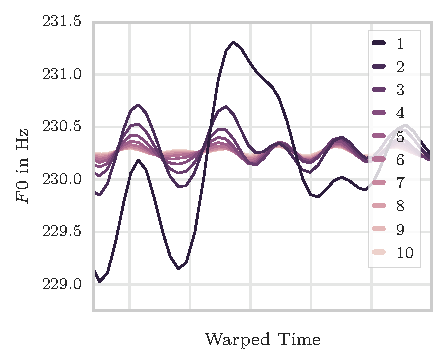
\includegraphics[width=.5\textwidth]{Chapters/05_Separation_Known/figures/f0_3d.pdf}};
\node[inner sep=0pt] (output) at (0,0) {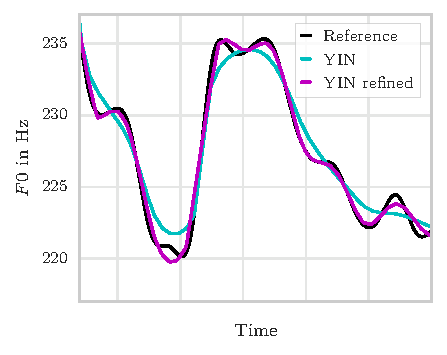
\includegraphics[width=.5\textwidth]{Chapters/05_Separation_Known/figures/output_f0.pdf}};
%
\end{tikzpicture}
\caption{$F0$ refinement for one excerpt of synthesized speech using \textbf{YIN}~\cite{decheveigne02} with 10 iterations. \emph{Left}: Estimated $F0$ in linear time. \emph{Right}: estimates after each warping iteration in warped time.}
\label{fig:teaser_refined}
\end{figure}

\subsection{Experiments and Evaluation} % (fold)
\label{sec:experiments}

For the evaluation of the proposed $F0$ refinement, we test the refinement algorithm with the following $F0$ estimators:\\
\textbf{YIN}~\cite{decheveigne02} is used as an FFT based implementation~\cite{bogdanov13}. The confidence measure is thresholded for values lower than 0.6 on the speech recordings. \textbf{iRAPT1,2}~\cite{azarov12} are improved versions of the RAPT framework. We use the author's MATLAB implementation of the iRAPT1 and iRAPT2 algorithms.\ iRAPT2 is a refinement method that is comparable to our proposed method. To evaluate the results, we apply our refinement to iRAPT1 and compare it with the refinement produced by iRAPT2. $c[n] < 0.7$ is used for thresholding speech recordings. \textbf{MELODIA}~\cite{salamon12} is not designed to be an $F0$ estimator but is able to extract the \emph{predominant} melody in a polyphonic mixture. We increase the bin resolution to 0.5 semitones, to increase the accuracy. We used the \textsc{Essentia} implementation. For thresholding we use the built-in voiced/unvoiced detection.
For YIN and MELODIA, we evaluate on a frame length of 64~ms and a hop size of 16~ms. For iRAPT1 and iRAPT2  we use the fixed frame length parameters of the author's implementation.
\par
We use the established evaluation measures \textsc{Gross Pitch Error} (GPE) and \textsc{Mean Fine Pitch Error} (MFPE)~\cite{azarov12}. We focus on MFPE in our results, measuring the absolute deviation of $F0_{\mathrm{true}}$ and the $F0$ estimate per sample.
As mentioned in~\cite{resch07}, evaluating the accuracy of $F0$ estimates is challenging because of the lack of ground truth datasets annotated on a time scale with such a high resolution. Most of the available audio test data sets are not suitable because the $F0$ annotation is only available with low time resolutions. By using such a dataset there is a risk that the refined $F0$ estimate is higher in MFPE. This is because the refined estimates show more of the fine structure deviating from the coarse annotation which then is considered as piecewise constant. To address this issue, we first present the evaluation results on synthetic data. To verify our synthetic results, we present the results of speech data annotated on 10~ms frames derived from laryngograph signals. We did only evaluate and process the voiced parts of the signals as indicated in the provided annotation labels. Also note that since we focus on the MFPE, all segments where one of the estimators results in a GPE $> 0$ are excluded from the results, hence the GPE for all of our results is 0. The proposed refinement has been processed with one iteration ($k=1$). Experiments showed that more iterations only marginally improve the results.

Since the proposed refinement algorithm repeatedly applies pitch estimation, the performance of these estimators on the time warped (nearly constant) signal is of interest. Therefore we included the results of an oracle refinement where the first estimate is set to a ground truth pitch. Additionally this also does reveal information about the quality of the ground truth annotation itself.

\subsubsection{Synthetic Data} % (fold)
\label{ssub:sythetic_data}

To generate synthetic test data we use pitch label annotations of the PTDB-TUG speech data set~\cite{pirker11}. We synthesize the melody or voice using a simple sinusoidal signal model. To get accurate ground truth data, the pitch annotations were up-sampled to audio rate by using linear interpolation for the PTDB-TUG. Similar to~\cite{mauch14}, we then synthesized the data using cosine based oscillators adding 10 harmonics to each signal output.
The test set has been rendered at 16 kHz. The complete PTDB-TUG set results in almost 10 hours of input signal data.
We present the results of the synthetic data as box plots in Figure~\ref{fig:ptdbtug_synth} grouped by estimator. It shows that all estimators benefit from the refinement in terms of MFPE. The iRAPT1 estimator shows the best improvement of \ptdbtugsynthiRAPTIMPROMFPE \% in MFPE. As expected, the Oracle Refinement is almost at 0 MFPE.

\begin{figure}[t!]
\centering
		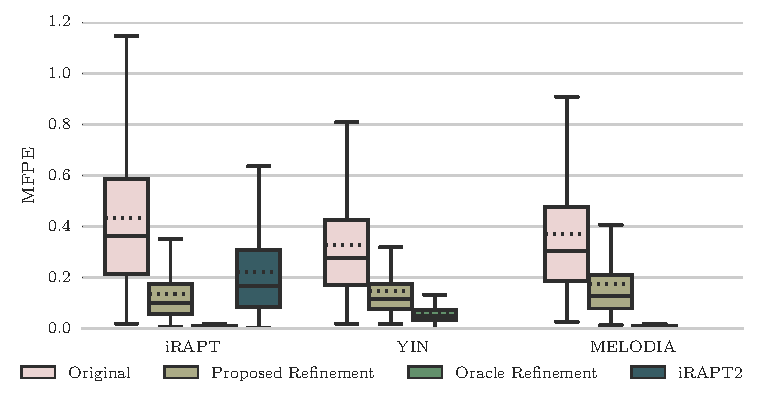
\includegraphics[width=0.90\columnwidth]{Chapters/05_Separation_Known/figures/stats_boxplot_ptdb_synth.pdf}
\caption{Results from the synthesized PTDB-TUG dataset. MFPE grouped by estimator. Solid/dotted lines represent medians/means. Outliers are not shown.}
\label{fig:ptdbtug_synth}
\end{figure}

\vspace{-0.6em}
\subsubsection{Speech Data} % (fold)
\label{ssub:speech}
For the results of the algorithm on real data we first used the same PTDB-TUG items as in the synthetic data but processed the accompanying speech recordings. The MFPE values were then calculated by averaging the sample wise $F0$ estimates from our proposed method over frame lengths of 10~ms to match the annotation data. The results are shown in Figure~\ref{fig:ptdbtug_real}. The mean values indicate that the MELODIA algorithm performs best overall. We can see that the refinement does not show a clear effect on the iRAPT estimator. The oracle refinement results indicate that even if a ground truth is known, the refinement based on the warped (constant) signal can not get much lower in MFPE. As also seen on synthetic data, iRAPT2 does not show any significant improvements compared to our proposed refinements.

\vspace{-0.6em}
\subsubsection{Polyphonic Mixtures} % (fold)
\label{ssub:polyphonic}

Pitch estimation of polyphonic mixture input signals in general is known to be more difficult than on monophonic signals. To show that our proposed refinement is not bound to the optimization on specific signals we processed the \mbox{MedleyDB}~\cite{MedleyDB} which consists of 108 professionally recorded music mixes where the main melody has been annotated by humans. We only evaluate the MELODIA~\cite{salamon14} estimator in this scenario. Frame lengths and hop sizes were increased to 92~ms and 23~ms, respectively. The set is processed at 44.1~kHz. To further back up the results of the fine pitch error in this scenario, we additionally evaluated the results of a correlation based measure as introduced in~\cite{resch07} (See Equation (19)). Instead of computing the correlation coefficients on the mixture, we used the accompanying multi-tracks. The track which most predominantly contributed to the main melody has been chosen for the correlation coefficient measure. The results of the experiment are shown in Figure~\ref{fig:medley}.

\begin{figure}[t!]
\centering
		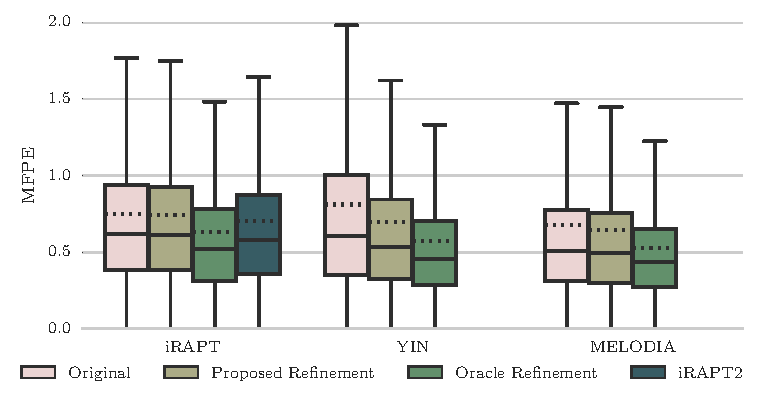
\includegraphics[width=0.90\columnwidth]{Chapters/05_Separation_Known/figures/stats_boxplot_ptdb_real.pdf}
\caption{Results from the real recordings PTDB-TUG dataset. MFPE grouped by estimator. Solid/dotted lines represent medians/means. Outliers are not shown.}
\label{fig:ptdbtug_real}
\end{figure}

\begin{figure}[t]
\centering
		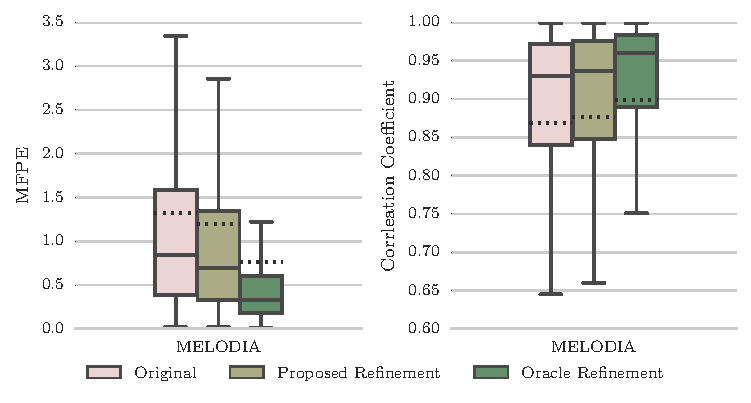
\includegraphics[width=0.90\columnwidth]{Chapters/05_Separation_Known/figures/stats_boxplot_medley.pdf}
\caption{Results from the real recordings MedleyDB dataset. MFPE and Correlation Coefficient grouped by estimator. Solid/dotted lines represent medians/means. Outliers are not shown.}
\label{fig:medley}
\end{figure}

\section{Summary and Discussion}

% [X] A summary of findings and limitations
% [X] Practical applications/implications
% [X] Recommendations for further research
% [X] Repeat the highlights of the chapter
% [X] Transition sentence that acts as a “teaser” for the next chapter

In this chapter, we highlighted the time-varying aspects of musical sources such as vibrato to be utilized for the application of source separation.
To address this task, we developed a method that utilizes time warping to extract a source from the mixture.
More specifically, the additional information is used to warp the mixture based on the fundamental frequency estimate of the source to be extracted. 
In the warped time domain the frequency modulation of the desired source is removed. 
In our first study, we evaluated this method on separating single note from instruments playing in unison.
For the actual separation, we used a standard NMF separation approach.
The results of 45 mixtures have been evaluated by using the PEASS toolbox and the scores indicated an improvement in favor of the F0 variation informed NMF compared to the standard NMF.
\par
In order to evaluate if our method can be applied on more realistic scenario, we proposed an extension of the method for the scenario of vocal/accompaniment separation.
We used a state-of-the-art melody estimation technique to extract the \(F0\) variation of the vocal source to apply warping to the mixture.
We performed separation in the time domain using a comb filter to further reduce artifact.
The method relies on a robust and accurate estimate of the fundamental frequency as well as vocal activity estimate.
\par
To address the latter, the method was extended to include a deep neural network based vocal activity detector.
This helped to exclude non-vocal parts from the warping and in turn, improved the vocal separation performance by 1.5~\si{\decibel} SDR.
In order to improve the accuracy of \(F0\) estimates, we proposed a method, based on the same time warping principle, in the last section of this chapter. 
The proposed method applies time warping iteratively based on an initial \(F0\) estimate, assuming that more iteration remove more variation, thus simplifies the \(F0\) estimation process.
This idea can be applied to any \(F0\) estimator as a post-processing step.
Future work could include an optimization criterion to control the number of iterations, however, we have to emphasize that improvements in accuracy are difficult to evaluate on real datasets~\cite{stoeter15acm}.
\par
To conclude, time warping based separation can work well on some signals but requires further hand crafted tuning to yield good results.
In the next chapter we want to investigate if separation can still benefit from spectro-temporal modulations if they are not known or estimated a priori.
\chapter{Separation by Unknown Modulation}
\label{cha:unknown}

In the previous chapter, methods were proposed to separate highly overlapped signals, informed by an estimate of fundamental frequency \(F0\) variation of the source to be separated.
Even though we showed that \(F0\)  variation could be estimated from the mixture, often, it is not easy to obtain in practice.
In contrast, in this chapter, we will introduce separation methods which do not incorporate prior knowledge about the modulation. 
In fact, some of the methods operate blindly, meaning they do not require any further information about the sources except for the number of sources to be separated.
\par
In blind source separation research, many contributions were based on non-negative matrix factorization (NMF)~\cite{lee99, lee01}.
NMF quickly became one of the main scientific frameworks in the field of audio source separation with a large number of contributions.
The popularity of NMF algorithms can be explained by the intuitive way in which they work on (non-negative) time-frequency representations of the mixture signal.
Let us consider the magnitude STFT \(\mX \in \sR_{+}^{F \times T}\) with \(F\) being the number of frequency bins and \(T\) the number of time frames.
Now, the NMF incorporates non-negative constraints to perform the separation into the sum of \(K\) latent components which are each factored into two matrices (referred to as frequency \emph{basis} \(\mW \in \sR_{+}^ { F \times K }\) and temporal \emph{activations} \(\mH \in \sR_{+}^ { T \times K }\)):

\begin{equation}
   \mathbf{X} \approx \mW \mH^{T} = \sum\limits_{k=1}^{K} \vw_{k} \circ \vh_{k}
   \label{eq:vanilla_nmf}
\end{equation}

As it can also be seen in Figure~\ref{fig:nmf}, the factorization can also be
written as the sum of \(K\) outer products between two rank-one matrices \(\vw_k \in \sR^F\)
and \(\vh_k \in \sR^T\).

\begin{figure}[ht]
  \centering
  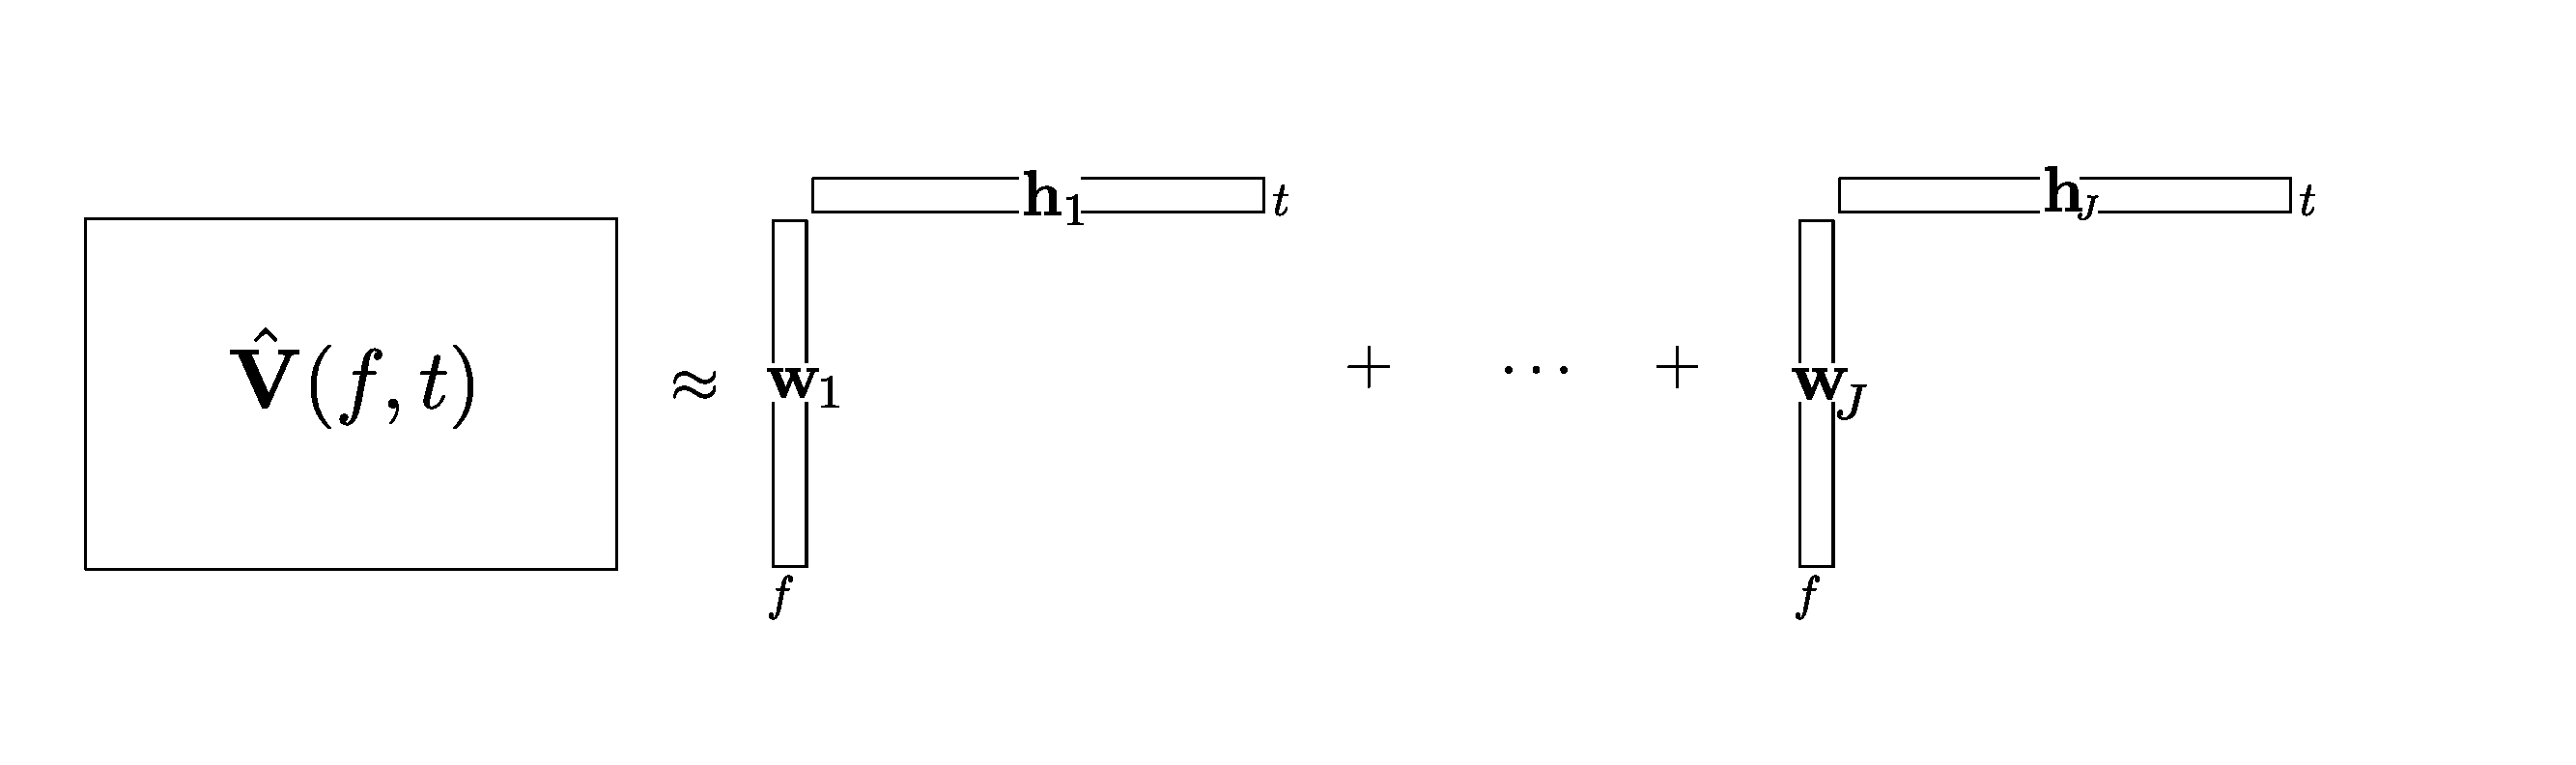
\includegraphics[width=0.9\textwidth]{Chapters/06_Separation_Unknown/figures/nmf.pdf}
  \caption{Visualization of the product of two rank-one matrices as being used in non-negative matrix factorization (NMF).}
  \label{fig:nmf}
\end{figure}

The NMF provides a rank reduction which allows decomposing mixtures into \(K\) source components.
At the same time, the factorization inherently follows specifics of music, observable in time-frequency representations: the fact that harmonic sources can be described using a pitch/tone (represented in \(\mW\)) and its duration (represented in \(\mH\)).
It is this property that also allowed to use NMF for the purpose of transcriptions~\cite{smaragdis03}.
\par
To obtain the factorization, an optimization problem needs to be solved, resulting in a non-unique solution.
Each factorization is calculated by minimizing the error between \(\mX\) and \(\mW \mH^{T}\) with respect to some cost function

\begin{equation}
  \min_{\mW,\mH^{T}} \mathrm{D}(\mX | \mW \mH) \text { subject to } \mW \geq 0 , \mathbf \mH \geq 0.
\end{equation}

In most source separation methods the beta-divergence cost function

\begin{equation}
  \mathrm{D}_{\beta} (x | y) = \frac { 1 } { \beta ( \beta - 1 ) } \left( x ^ { \beta } + ( \beta - 1 ) y ^ { \beta } - \beta x y ^ { \beta - 1 } \right) \quad \beta \in \mathbb { R } \backslash \{ 0, 1 \}
\end{equation}

is being used~\cite{fitzgerald08a}. 
For the special cases of \(\beta = 0\) and \(\beta = 1\), \(\mathrm{D}\) correspond to the Itakura-Saito (IS) and Kullback-Leibler (KL) divergence and the euclidean distance equals to (\(\beta = 2\)).
To efficiently compute the optimization, an algorithm was proposed in~\cite{lee01} which makes use of simple to use multiplicative update rules, derived from the cost function.
For further details, we refer to~\cite{cichoki09}.
\par
After factorizing \(\mX\) into \(K\) components, one can obtain \(K\) magnitude spectra.
However, \(K\) is usually selected to be larger or equal to the total number of sources.
When it is larger than the number of sources, the components can be clustered into the number of desired sources.
Often this can be achieved by some similarity metric that allows to calculate pairwise distances between the \(K\) components and the desired sources and apply \textit{k}-means clustering algorithm~\cite{spiertz09}.
A separation example is depicted in Figure~\ref{fig:nmf_separation}. 
Here the number of components \(K\) is six per sources, resulting in a total number of \(K=12\). 
Each component is clustered into one of two sources to generate two estimates.

\begin{figure}[h]
  \centering
  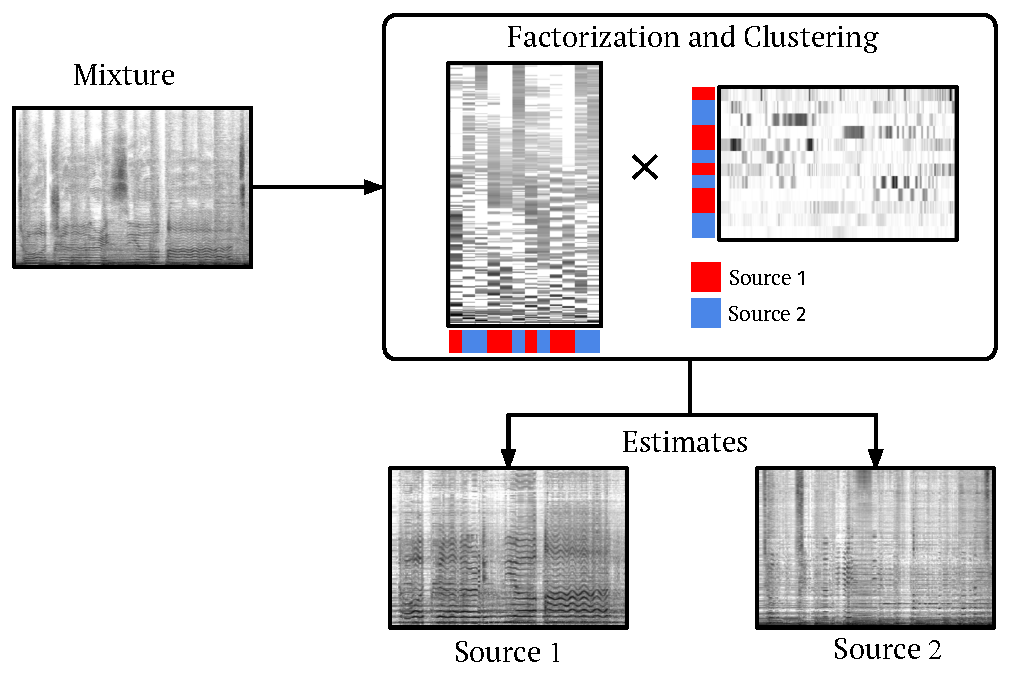
\includegraphics[width=0.8\textwidth]{Chapters/06_Separation_Unknown/figures/nmf_separation.pdf}
  \caption{Example of spectrogram based source separation using non-negative matrix factorization (NMF).}
  \label{fig:nmf_separation}
\end{figure}

It is this step that transforms the NMF into a supervised algorithm.
As for other separation methods, performed in the time-frequency domain, separation is achieved using Wiener filters or soft masks to extract the sources from the mixture~\cite{liutkus15c}.
\par
Since NMF first appeared to the source separation community in~\cite{smaragdis03} and in~\cite{vembu05}, a large variety of NMF ``flavors'' were introduced to improve certain aspects of the NMF in the application of music. 
In~\cite[Chapter 16]{vincent} of that book the authors describe one of the main problems of NMF which is that ``standard NMF is shown to be effective when the notes of the analyzed music signal are nearly stationary''.
As we described in Chapter~\ref{cha:highly-overlapped-signals}, this is especially important for pitches that incorporate vibrato.
Here, NMF-based processing suffers from its simplified model and its magnitude STFT representation makes it harder to model these time-varying sources.
\par
To underpin this issue, we depict this problem in Figure~\ref{fig:am_tensor_nmf} which shows the factorization of a simple amplitude modulated input signal. 
The signal consists of two sinusoids which are linearly mixed. 
Both share the same carrier frequency but have different amplitude modulation rates. 
When we apply a factorization with $K=2$, one can see that NMF has difficulties to separate the two signals sufficiently and instead activates both sources in an alternating pattern.

\begin{figure}[H]
\centering
\subcaptionbox{Time Domain}%
[1\textwidth]{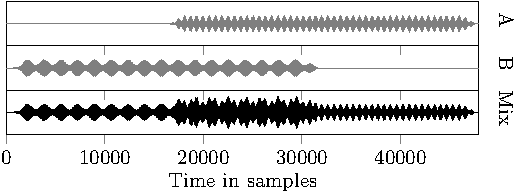
\includegraphics[width=0.7\textwidth]{Chapters/05_Separation_Known/figures/Timepdf-crop.pdf}}%
\hspace{0.2\textwidth} % separation
\subcaptionbox{Magnitude STFT}
[1\textwidth]{% This file was created by matlab2tikz% This file was created by matlab2tikz v0.4.7 (commit 3442858e5a642c135c5e9dab6a960bee5b9c6f8d) running on MATLAB 8.2.
% Copyright (c) 2008--2014, Nico Schlmer <nico.schloemer@gmail.com>
% All rights reserved.
% Minimal pgfplots version: 1.3
%
% The latest updates can be retrieved from
%   http://www.mathworks.com/matlabcentral/fileexchange/22022-matlab2tikz
% where you can also make suggestions and rate matlab2tikz.
%
\begin{tikzpicture}[font=\small]

\begin{axis}[%
width=0.15\columnwidth,
height=3.5cm,
axis on top,
xminorgrids=true,
minor xtick={1.5,2.5},
scale only axis,
xtick={1,2},
xmin=0.5,
xmax=2.5,
ymin=0.5,
ymax=137.5,
name=plot2,
xlabel=Gain Components,
ylabel=Modulation Frequency Bins,
every axis y label/.style={at={(current axis.north east)},below=18mm,xshift=8mm},
y label style={rotate=-90},
]
\addplot [forget plot] graphics [xmin=0.5,xmax=2.5,ymin=0.5,ymax=137.5] {Chapters/05_Separation_Known/figures/AMPlots/GAS-1_scaled.png};
\end{axis}

\begin{axis}[%
width=0.15\columnwidth,
height=3.5cm,
xminorgrids=true,
minor xtick={1.5,2.5},
axis on top,
scale only axis,
xtick={1,2},
xmin=0.5,
xmax=2.5,
ymin=0.5,
ymax=145.5,
xlabel=Basis Components,
ylabel=Frequency Bins,
every axis y label/.style={at={(current axis.north east)},below=18mm,xshift=8mm},
y label style={rotate=-90},
at=(plot2.left of south west),
anchor=right of south east
]
\addplot [forget plot] graphics [xmin=0.5,xmax=2.5,ymin=0.5,ymax=145.5] {Chapters/05_Separation_Known/figures/AMPlots/GAS-2_scaled.png};
\end{axis}

\begin{axis}[%
width=0.15\columnwidth,
height=3.5cm,
xminorgrids=true,
minor xtick={1.5,2.5},
axis on top,
scale only axis,
xtick={1,2},
xmin=0.5,
xmax=2.5,
ymin=0.5,
ymax=81.5,
xlabel=Activation Components,
ylabel=Frames,
every axis y label/.style={at={(current axis.north east)},below=18mm,xshift=8mm},
y label style={rotate=-90},
at=(plot2.right of south east),
anchor=left of south west
]
\addplot [forget plot] graphics [xmin=0.5,xmax=2.5,ymin=0.5,ymax=81.5] {Chapters/05_Separation_Known/figures/AMPlots/GAS-3_scaled.png};
\end{axis}
\end{tikzpicture}%
 v0.4.7 (commit 3442858e5a642c135c5e9dab6a960bee5b9c6f8d) running on MATLAB 8.2.
% Copyright (c) 2008--2014, Nico Schlmer <nico.schloemer@gmail.com>
% All rights reserved.
% Minimal pgfplots version: 1.3
%
% The latest updates can be retrieved from
%   http://www.mathworks.com/matlabcentral/fileexchange/22022-matlab2tikz
% where you can also make suggestions and rate matlab2tikz.
%
\begin{tikzpicture}[font=\small]

\begin{axis}[%
    /pgf/number format/.cd,
           use comma,
           1000 sep={},
width=0.35\columnwidth,
height=3.5cm,
axis on top,
scale only axis,
xmin=0.5,
xmax=1497.5,
ymin=0.5,
ymax=145.5,
xlabel=Frames,
ylabel=Frequency Bins,
every axis y label/.style={at={(current axis.north east)},below=18mm,xshift=4mm},
y label style={rotate=-90},
]
\addplot [forget plot] graphics [xmin=0.5,xmax=1497.5,ymin=0.5,ymax=145.5] {Chapters/05_Separation_Known/figures/AMPlots/STFT-1_scaled.png};
\end{axis}
\end{tikzpicture}%
}%
\hspace{0.3\textwidth} % separation
\subcaptionbox{Factorization}
[1\textwidth]{% This file was created by matlab2tikz v0.4.7 (commit 3442858e5a642c135c5e9dab6a960bee5b9c6f8d) running on MATLAB 8.2.
% Copyright (c) 2008--2014, Nico Schlmer <nico.schloemer@gmail.com>
% All rights reserved.
% Minimal pgfplots version: 1.3
%
% The latest updates can be retrieved from
%   http://www.mathworks.com/matlabcentral/fileexchange/22022-matlab2tikz
% where you can also make suggestions and rate matlab2tikz.
%
\begin{tikzpicture}[font=\small]

\begin{axis}[%
/pgf/number format/.cd, use comma, 1000 sep={},
width=0.225\columnwidth,
height=3.5cm,
axis on top,
scale only axis,
xtick={1,2},
xminorgrids=true,
minor xtick={1.5},
xmin=0.5,
xmax=2.5,
ymin=0.5,
ymax=145.5,
name=plot1,
xlabel=Basis Components,
ylabel=Frequency Bins,
every axis y label/.style={at={(current axis.north east)},below=18mm,xshift=8mm},
y label style={rotate=-90},
]
\addplot [forget plot] graphics [xmin=0.5,xmax=2.5,ymin=0.5,ymax=145.5] {Chapters/05_Separation_Known/figures/AMPlots/WH-1_scaled.png};
\end{axis}

\begin{axis}[%
/pgf/number format/.cd, use comma, 1000 sep={},
width=0.225\columnwidth,
height=3.5cm,
axis on top,
scale only axis,
xminorgrids=true,
minor xtick={1.5},
xtick={1,2},
xmin=0.5,
xmax=2.5,
ymin=0.5,
ymax=1497.5,
xlabel=Activation Components,
ylabel=Frames,
every axis y label/.style={at={(current axis.north east)},below=18mm,xshift=8mm},
y label style={rotate=-90},
at=(plot1.right of south east),
anchor=left of south west
]
\addplot [forget plot] graphics [xmin=0.5,xmax=2.5,ymin=0.5,ymax=1497.5] {Chapters/05_Separation_Known/figures/AMPlots/WH-2_scaled.png};
\end{axis}
\end{tikzpicture}%
}%
\caption{Example of separating a mixture of two amplitude modulated (AM) sinusoids using non-negative matrix factorization (NMF)\\ \textbf{(a)} Mixture of two sinusoids at $440$ Hz with AM of $4.7$ Hz and $12.6$ Hz (sample rate=$8$ kHz), \textbf{(b)} STFT (FFT length = 256), \textbf{(c)} Non-negative matrix factorization results in $\mW$ and $\mH$, after 100 iterations ($\beta = 1$).}
\label{fig:am_tensor_nmf}
\end{figure}

One way towards better separation is to increase the number of components per source, however, this introduces difficulties in the clustering.
Another method is proposed in~\cite{smaragdis04, fitzgerald05s, jaiswal13, rodriguezserrano16} which use convolutions to model shifts in components.
This lead to factorizations that are able to also model vibrato events.
However as stated in~\cite{hennequin11}, it does ``not  permit  any variation  between  different  occurrences  of  the  same event (atom), its duration and spectral content evolution being fixed''. 
Instead, they proposed a frequency-dependent activation matrices by using a source/filter-based model.
The model is based on an Auto-Regressive Moving Average (ARMA) time-varying model that allows single spectral components to be modeled along with their spectral variations. 
The model, as reported by the authors, however, does only allow for small frequency variations and fitting the ARMA model is a time-consuming process.

\section{Tensor Factorizations for Modulation Spectrograms}
\label{sub:am}

\marginpar{Parts of this subsection is also based on the work published in~\cite{stoeter14}.}

Another way to improve separation of modulated sources is the use of higher-dimensional tensor representations.
A variety of models exist to factorize a tensor into three components and apply a similar rank reduction as in the NMF case.
Tensor factorizations are useful for applications of data with more than two dimensions.
In audio separation, tensor factorization were originally proposed to address multichannel separation as in~\cite{fitzgerald08, fevotte10, ozerov11}. 
Barker and Virtanen~\cite{barker13} were the first to propose a modulation tensor representation for single-channel source separation. 
Their use of modulation spectra helps to identify amplitude modulations such as the one (indirectly) caused by vibrato. 
A complete signal representation is obtained by a modulation tensor which holds the modulation spectrograms for each time frame.
The modulation spectrogram tensor is a time-frequency-frequency representation of a time domain input signal.
The modulation spectrogram has already gathered much attention in speech recognition~\cite{greenberg97, kingsbury98} and classification~\cite{kinnunen08, markaki09} as introduced in Chapter~\ref{cha:fundamentals}.
\par
In practice, the modulation tensor \(\mathbf{V}_{f, b, t}\) , where \(b\) represents the modulation index, can be computed from the (magnitude) time frequency matrix \(\mathbf{X}_{f, t}\) by computing \(f\) time frequency transforms over each frequency band of \(\mathbf{X}\).
As proposed by~\cite{barker13}, the non-negative tensor factorization approximates a modulation tensor \(\mV\) by a product of three matrices containing the frequency/basis \(\mW\), time/activation \(\mH\) signals, and the modulation gain for each component \(\mM\).
The product of this factorization is generally referred to as \emph{PARAFAC} product\footnote{Also known as ``Polyadic form of a tensor'', PARAFAC (parallel factors), CANDECOMP or CAND (canonical decomposition) or CP (CANDECOMP/PARAFAC)~\cite{kolda09}.}.

In the vein of the NMF factorization mentioned in Equation~\ref{eq:vanilla_nmf}, a 3-way NTF can simply be extended to:

\begin{equation}
   \mathbf{V} \approx \sum\limits_{k=1}^{K} \mathbf{w}_{k}(f) \circ \mathbf{m}_{k}(b) \circ \mathbf{h}_{k}(t).
\end{equation}

This notation is commonly used in many tensor factorization applications~\cite{kolda09}.
However, we found that it is easier to follow when the individual tensor elements are used, which is also the recommended notation proposed in~\cite{kiers00}, for  $f = 1,\ldots,F; b=1,\ldots,B;t=1,\ldots,T$:

\begin{equation}
  v_{fbt} \approx \sum_{k = 1}^{K} w_{fk} m_{bk} h_{tk}.
\end{equation}

A visualization of the three-way PARAFAC product is depicted in Figure~\ref{fig:cpd}.

\begin{figure}[!t]
  \centering
  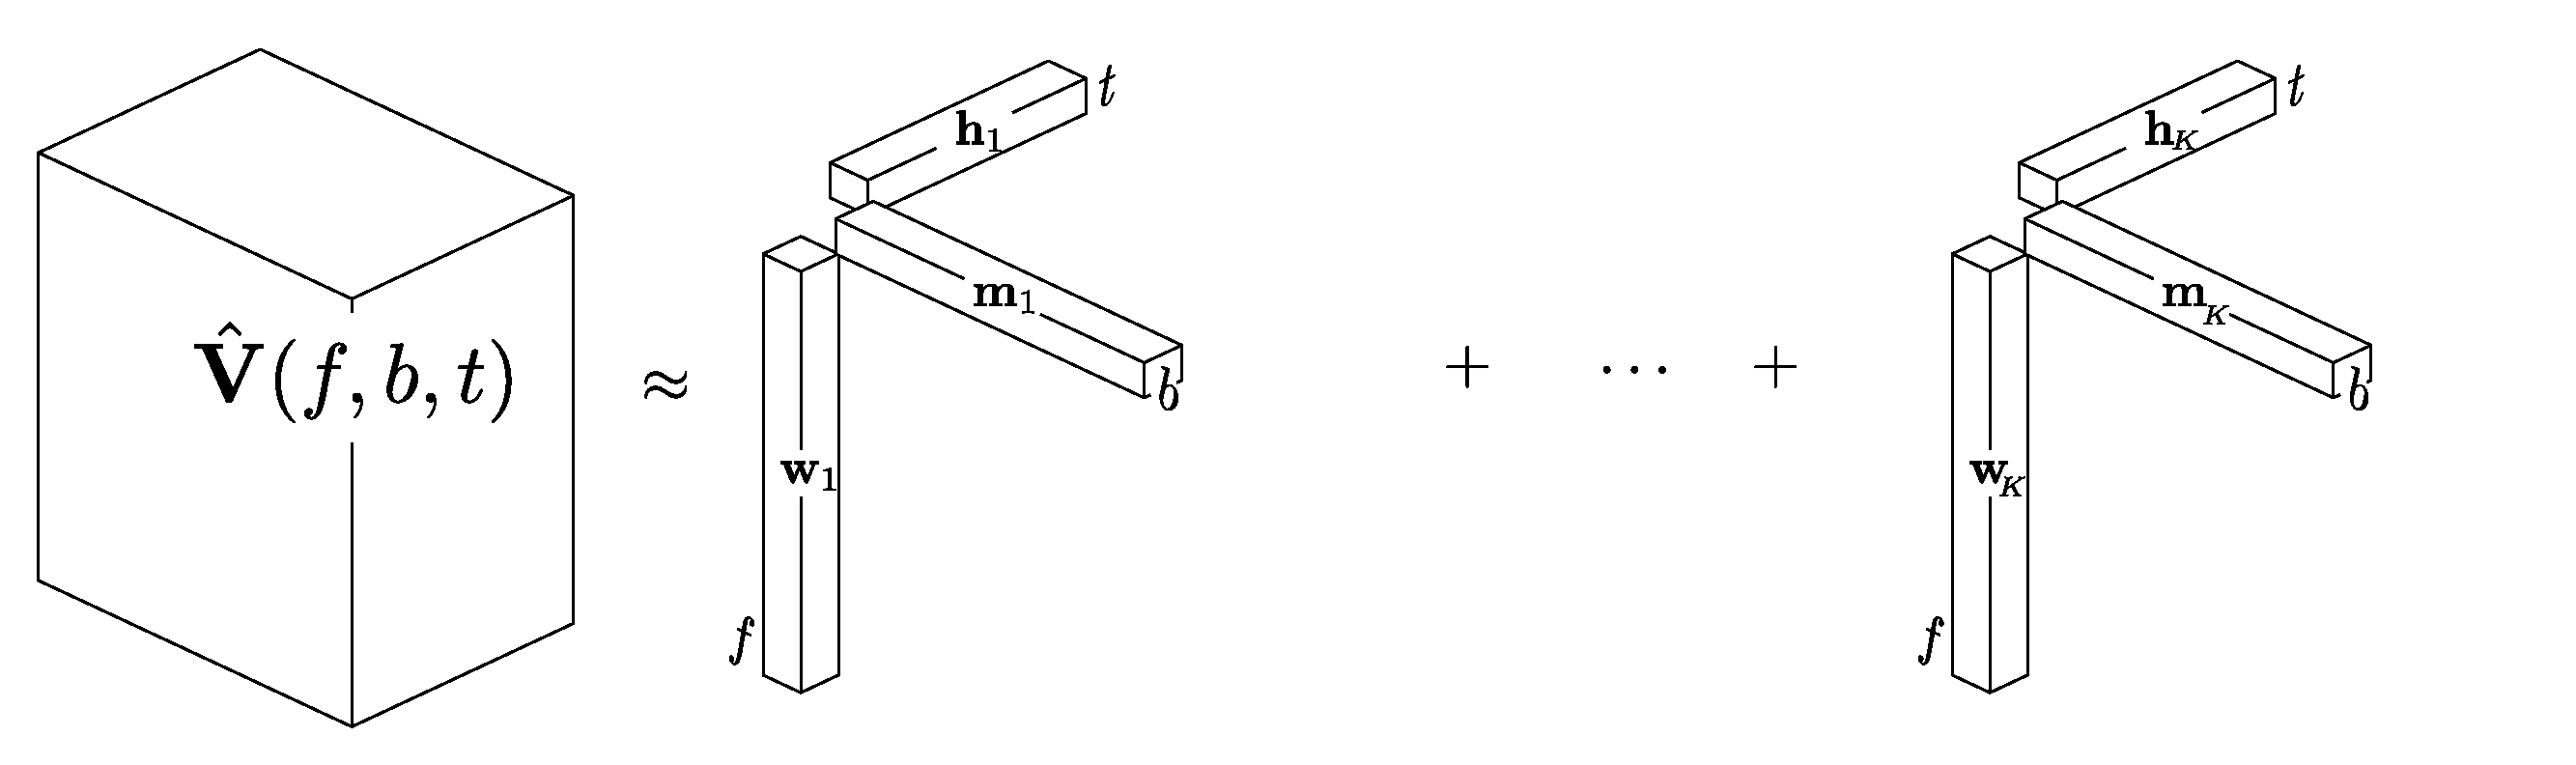
\includegraphics[width=1\textwidth]{Chapters/06_Separation_Unknown/figures/cpd.pdf}
  \caption{PARAFAC decomposition in an example for a three-dimensional tensor \(\mV\) into the sum of \(K\) outer products of three rank-one matrices.}
  \label{fig:cpd}
\end{figure}

% we implemented a custom C++ version of the PARAFAC product.
% we included Parallelisation, SIMD Vectorized and it is Cache Optimized
%
% Depending on the data size, between 20 and 40 times faster than a Python implementation of the same operation!  Also found that in the original algorithm, it is not necessary to perform
%
% this product for every factor, but only for each iteration !  This implementation can be used not only for Beta-NTF but also for
% many other algorithms using PARAFAC or CANDECOMP
\par
Compared to Barker and Virtanen in~\cite{barker13}, we chose to generate the modulation tensor in a way that is simpler and easier to invert. 
They used a Gammatone filter bank and rectification to model the characteristics of the human auditory system. 
We simplified the processing and used a two-stage DFT filter bank where the modulation domain is based on magnitude STFT. 
Although this can give perceptually less optimal results, each step can be directly inverted by using the complex representation.
Barker already showed that the NTF based approach gives good results on speech signals compared to the ``standard'' NMF. 
Motivated by these results, we wondered if the modulation NTF can be used to separate two instrument mixtures by their amplitude modulation characteristics, as it is the case in the unison scenario.
\par
Thus, let us return to the example from Figure~\ref{fig:am_tensor_nmf} of two harmonic signals having the same fundamental frequency of 440~\si{\hertz}, with a stationary amplitude of 4~\si{\hertz} and 10~\si{\hertz} respectively. 
These differences now turn out to be latent in a non-negative modulation tensor representation.
In contrast to NMF, Figure~\ref{fig:am_ntf} shows valid factorizations of a unison signal using NTF.
It gives a smoother activation matrix and is able to generate the output with the separated amplitude modulations on each sinusoid. The modulation frequency gain matrix shows the two modulation frequency templates and the DC-component.

\begin{figure}[!h]
\centering
% \subcaptionbox{Time Domain}%
% [1\textwidth]{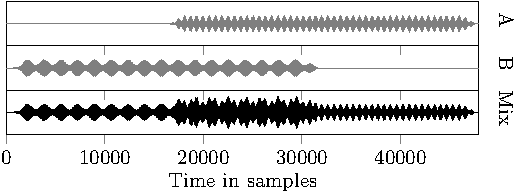
\includegraphics[width=0.8\textwidth]{Chapters/05_Separation_Known/figures/Timepdf-crop.pdf}}%
% \hspace{0.2\textwidth} % separation
\subcaptionbox{Slice of Modulation Tensor}
[1\textwidth]{% This file was created by matlab2tikz v0.4.7 (commit 3442858e5a642c135c5e9dab6a960bee5b9c6f8d) running on MATLAB 8.2.
% Copyright (c) 2008--2014, Nico Schlmer <nico.schloemer@gmail.com>
% All rights reserved.
% Minimal pgfplots version: 1.3
%
% The latest updates can be retrieved from
%   http://www.mathworks.com/matlabcentral/fileexchange/22022-matlab2tikz
% where you can also make suggestions and rate matlab2tikz.
%
\begin{tikzpicture}[font=\small]

\begin{axis}[%
width=0.35\columnwidth,
height=3.5cm,
axis on top,
scale only axis,
xmin=0.5,
xmax=81.5,
ymin=0.5,
ymax=137.5,
xlabel=Frames,
ylabel=Modulation Frequency Bins,
every axis y label/.style={at={(current axis.north east)},below=18mm,xshift=4mm},
y label style={rotate=-90},
]
\addplot [forget plot] graphics [xmin=0.5,xmax=81.5,ymin=0.5,ymax=137.5] {Chapters/05_Separation_Known/figures/AMPlots/Tmod-1_scaled.png};
\end{axis}
\end{tikzpicture}%
}%
\hspace{0.3\textwidth} % separation
\subcaptionbox{Tensor Factorization}
[1\textwidth]{% This file was created by matlab2tikz v0.4.7 (commit 3442858e5a642c135c5e9dab6a960bee5b9c6f8d) running on MATLAB 8.2.
% Copyright (c) 2008--2014, Nico Schlmer <nico.schloemer@gmail.com>
% All rights reserved.
% Minimal pgfplots version: 1.3
%
% The latest updates can be retrieved from
%   http://www.mathworks.com/matlabcentral/fileexchange/22022-matlab2tikz
% where you can also make suggestions and rate matlab2tikz.
%
\begin{tikzpicture}[font=\small]

\begin{axis}[%
width=0.15\columnwidth,
height=3.5cm,
axis on top,
xminorgrids=true,
minor xtick={1.5,2.5},
scale only axis,
xtick={1,2},
xmin=0.5,
xmax=2.5,
ymin=0.5,
ymax=137.5,
name=plot2,
xlabel=Gain Components,
ylabel=Modulation Frequency Bins,
every axis y label/.style={at={(current axis.north east)},below=18mm,xshift=8mm},
y label style={rotate=-90},
]
\addplot [forget plot] graphics [xmin=0.5,xmax=2.5,ymin=0.5,ymax=137.5] {Chapters/05_Separation_Known/figures/AMPlots/GAS-1_scaled.png};
\end{axis}

\begin{axis}[%
width=0.15\columnwidth,
height=3.5cm,
xminorgrids=true,
minor xtick={1.5,2.5},
axis on top,
scale only axis,
xtick={1,2},
xmin=0.5,
xmax=2.5,
ymin=0.5,
ymax=145.5,
xlabel=Basis Components,
ylabel=Frequency Bins,
every axis y label/.style={at={(current axis.north east)},below=18mm,xshift=8mm},
y label style={rotate=-90},
at=(plot2.left of south west),
anchor=right of south east
]
\addplot [forget plot] graphics [xmin=0.5,xmax=2.5,ymin=0.5,ymax=145.5] {Chapters/05_Separation_Known/figures/AMPlots/GAS-2_scaled.png};
\end{axis}

\begin{axis}[%
width=0.15\columnwidth,
height=3.5cm,
xminorgrids=true,
minor xtick={1.5,2.5},
axis on top,
scale only axis,
xtick={1,2},
xmin=0.5,
xmax=2.5,
ymin=0.5,
ymax=81.5,
xlabel=Activation Components,
ylabel=Frames,
every axis y label/.style={at={(current axis.north east)},below=18mm,xshift=8mm},
y label style={rotate=-90},
at=(plot2.right of south east),
anchor=left of south west
]
\addplot [forget plot] graphics [xmin=0.5,xmax=2.5,ymin=0.5,ymax=81.5] {Chapters/05_Separation_Known/figures/AMPlots/GAS-3_scaled.png};
\end{axis}
\end{tikzpicture}%
}%
\caption{\textbf{(a)} Modulation tensor slice of a mixture of two sinusoids at $440$ Hz with AM of $4.7$ Hz and $12.6$ Hz (sample rate=$8$ kHz)  (FFT length = 256), \textbf{(b)}  $\mV \approx \mW \mM \mH$ Result of Non-Negative Tensor Factorization ($\beta = 1$) after 100 iterations}
\label{fig:am_ntf}
\end{figure}
\par
A comparison of the modulation tensor approach compared to the \(F0\) variation informed method on the unison separation scenario has been carried out in our work published in~\cite{stoeter14}.
Results indicated that the modulation tensor factorization generally performs worse than informed methods.
This is because it only considers amplitude modulations even though frequency modulations are the
the actual source of the modulation.
In the next section, we investigated how more complex modulation patterns can be utilized for separation.

\section{Common Fate Model for Unison Mixtures}%
\label{sec:the_common_fate_model_for_unison_mixtures}

\marginpar{This section was previously published in~\cite{stoeter16} and was revised for this thesis with permission (\textsuperscript{\textregistered}2016 IEEE).}

In this work, a novel tensor signal representation is introduced which additionally exploits similarities in the frequency direction.
We, therefore, make use of dependencies between modulations of neighboring bins.
This is similar to the proposed high-resolution non-negative Matrix Factorization model that accounts for dependencies in the time-frequency plane (HR-NMF~\cite{badeau11}).
In short, HR-NMF models each complex entry of a time-frequency transform of an audio signal as a linear combination of its neighbors, enabling the modeling of damped sinusoids, along with an independent innovation.
This model was generalized to multichannel mixtures in~\cite{badeau13a, badeau14} and was shown to provide considerably better oracle performance for source separation than alternative models in~\cite{magron15a}.
Indeed, even though some variational approximations were introduced in~\cite{badeau13} to strongly reduce their complexity, those algorithms are often demanding for practical applications.
In this work, we proposed to relax some assumptions of HR-NMF in the interest of simplifying the estimation procedure.
The core idea is to divide the complex spectrogram into modulation patches in order to group common modulation in time and frequency direction.
We call this the \emph{Common Fate Model} (CFM), borrowing from the Gestalt theory, which describes how human perception merges objects that move together over time (from~\cite{bregman90}):

\begin{quote}
``the Gestalt psychologists discovered that when different parts of the perceptual field were changing in the same way at the same time, they tended to be grouped together and seen to be changing as a group because of their common fate.'' 
\end{quote}

Bregman introduced the Common Fate theory for auditory scene analysis as the ability to group sound objects based on their common motion over time, as occurs with frequency modulations of harmonic partials.
As outlined by Bregman, the human ability to detect and group sound sources by small differences in FM and AM is outstanding.
Also, it turns out, as mentioned in Section~\ref{exploiting-slow-modulations}, that humans are especially sensitive to modulation frequencies around 5~Hz, which is the typical vibrato frequency that many musicians produce naturally.

\subsection{The Common Fate Transform}
\label{sub:CFT}

Let $\tilde{x}$ denote a single channel audio signal.
Its Short-Term Fourier Transform (STFT) is computed by splitting it into overlapping frames and then taking the discrete Fourier transform (DFT) of each one.
Since the waveform~$\tilde{x}$ is real, the Fourier transform of
each frame is Hermitian. In the following, we assume that the redundant
information has been discarded to yield the STFT.
The resulting information is gathered into an $N_{\omega}\times N_{\tau}$
matrix written~$\mX$, where~$N_{\omega}$ is the number of frequency
bands and $N_{\tau}$ the total number of frames.
In this study, we will consider the properties of another object, built from $\mX$, which we call the Common Fate Transform (CFT).
\par
It is constructed as illustrated in Figure~\ref{fig:CFT}.
We split the STFT~$\mX$ into overlapping rectangular $N_{a}\times N_{b}$ patches, regularly spaced over both time and frequency.
For reference, later in this thesis, we will call this representation the \emph{Grid STFT} (GFT).
Then, the 2D-DFT of each patch is computed\footnote{Note that since each patch is complex, its 2D-DFT is not Hermitian, thus all its entries are kept.}.
This yields an $N_{a}\times N_{b}\times N_{f}\times N_{t}$ tensor where~$N_{f}$ and~$N_{t}$ are the vertical and horizontal positions for the patches, respectively.
\par
As can be seen, the CFT is basically a further short-term 2D-DFT taken over the ``standard'' STFT~$\mX$.
One of the main differences compared to modulation spectrograms is that the CFT is computed using the complex STFT~$\mX$, and not a magnitude representation such as $\left|\mX\right|$.
As we will show, this simple difference has many interesting consequences, notably that the CFT is invertible: the original waveform~$\tilde{x}$ can be exactly recovered by cascading two classical overlap-add procedures.
Another difference is that the patches span several frequency bins, \emph{i.e.} we may have~$N_{a}>1$.
This contrasts with the conventional modulation spectrogram, that is defined using one frequency band only.

\begin{figure}[t]
\centering
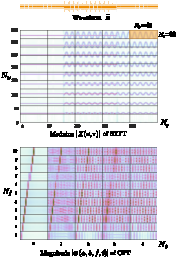
\includegraphics[width=0.8\textwidth]{Chapters/06_Separation_Unknown/figures/CFT}
\caption{Common Fate Transform. For convenience, the splitting of the STFT
into patches has been depicted without overlap, but overlapping patches are used in practice\label{fig:CFT}. \textsuperscript{\textregistered}2016 IEEE.}
\end{figure}

\subsubsection{A Probabilistic Model for the CFT}

\label{ssub:separation}

When processing an audio signal~$\tilde{x}$ for source separation,
it is very common to assume that all time-frequency (TF) bins
of its STFT are independent~\cite{fevotte09, duong10, ozerov12, liutkus11t}.
This is often the consequence of two different assumptions.
The first one is to consider that all frames are independent, thus
leading to the independence of all entries of the STFT that do not belong to the
same column. The second one is related to the notion of stationarity:
roughly speaking, the Fourier transform is known to decompose stationary
signals into independent components.
As a consequence, when the signals are assumed to be \emph{locally stationary},
it is theoretically sound to assume that all the entries of
their STFT are independent.

Still, both assumptions can only be considered as approximations.
First, adjacent frames are obviously not independent, notably because
of the overlap between them. Second, the stationarity assumption is
only approximate in practice, especially when percussive elements are
found in the audio, leading to strong dependencies among the different
frequency bins. Let $\{ \mX_{ft}\} _{f,t}$
denote all the $N_{a}\times N_{b}$ patches taken on the STFT to compute
the CFT, as depicted in Figure~\ref{fig:CFT}. The probabilistic
model we choose is the combination of \emph{three} different assumptions
made on the distribution of these patches\footnote{A forth assumption made in~\cite{stoeter16} refers to the joint distribution of all entries of each patch which are $\alpha$-stable~\cite{samoradnitsky94}.}.

\begin{enumerate}[leftmargin=0cm,itemindent=.5cm,labelwidth=\itemindent,labelsep=0cm,align=left]
\item All patches are independent. 
Just as the classical locally stationary
model~\cite{liutkus11t} assumes independence of overlapping frames,
we assume here independence of overlapping patches. Due to the
overlap between them, this assumption is an approximation,
and one may wonder what the advantage is of dropping independent frames
for independent patches. 
The answer lies in the fact that the latter permits us to model phase dependencies between neighboring STFT entries, and also to model much longer-term dependencies, as required for instance by deterministic damped or frequency-modulated sinusoidal signals.\label{enu:assumption_independent_patches}
\item Each patch is \emph{stationary}: its distribution
is assumed invariant under translations in the TF plane. This is where we do not assume independence, but on the contrary, expect dependencies among neighboring STFT entries. Our approach assumes this happens in a way that only depends on the relative positions in
the TF plane. It can easily be shown that mixtures of
damped sinusoids have this property. Assuming stationarity not only over time but over both time and frequency
also permits us to naturally account for mixtures of frequency-modulated
sounds. In short, we assume that throughout each patch, we observe
one coherent STFT ``texture''. The difference with the HR-NMF model is that we have independent and identically
distributed (i.i.d.) innovations for one given patch, whereas HR-NMF model has more variability. 
However, taking overlapping patches somehow compensates for
this limitation.\label{enu:assumption_stationary}
% \item The joint distribution of all entries of each patch is $\alpha$-stable~\cite{samoradnitsky94}.
% $\alpha$-stable distributions are the only ones that are stable under additions, \emph{i.e.} such that
% sums of $\alpha$-stable random variables (r.v.) remain $\alpha$-stable.
% They notably comprise the Gaussian and Cauchy distributions as special
% cases when $\alpha=2$ and $\alpha=1$, respectively.\label{enu:assumption_alpha_stable}
\item All entries of the Fourier transform of each patch
are assumed to be asymptotically independent, as the size of the patch
gets larger. This rather technical condition, often tacitly made in
signal processing studies, permits efficient processing in the frequency
domain.\label{enu:assumption_harmonisable}
\end{enumerate}

Under those assumptions, all entries of the CFT are independent
(assumptions~\ref{enu:assumption_independent_patches} and~\ref{enu:assumption_stationary})\footnote{This result is the direct generalization
of~\cite[th. 6.5.1]{samoradnitsky94} to multi-dimensional stationary processes.}
where $P\left(a,b,f,t\right)$ is a non-negative Tensor with dimensions $N_{a}\times N_{b}\times N_{f}\times N_{t}$
 that we call the \emph{modulation density}. In
the general case, it can basically be understood as the energy found at $\left(a,b\right)$ for patch
$\left(f,t\right)$, just like more classical power spectral
densities describe the spectro-temporal energy content of the STFT
of a locally stationary signal.

\subsubsection{Interpretation of the CFT as Filterbank}
\label{sub:interpretation}

An alternative interpretation of the CFT can be obtained by regarding the 2D-DFT
as two subsequent 1D-DFTs. If the transform in frequency direction (DFT-F) is
applied first, it is equivalent to a partial inverse DFT plus time reversal. If
the time reversal would be undone and an overlap-add would be applied, the
output would correspond to a subband representation with a frequency resolution
of $N_\omega / N_a$. Each of the $N_a$ final transformations (DFT-T) in one
patch takes output values from $N_b$ DFT-Ts with equal indices. This corresponds
to a splitting into poly-phase components with downsampling factor $N_a$ of the
time signal obtained by placing the output frames from the DFT-Ts in a row.
Thus, the outputs of the DFT-Fs have a very high frequency resolution of
$N_\omega N_b$ but contain aliasing components from the downsampling.
\par
This interpretation of the CFT gives some indications for its benefits in the
separation of modulated sources. Due to the poly-phase representation, it has a
relatively high temporal resolution. The periodicities in the spectra caused
by downsampling make the CFT relatively independent of frequency shifts, so
that, for example, the output patch of a single sinusoidal sweep is mainly
influenced by the sweep rate.

\subsection{Signal Separation}
Now, let us assume that the observed waveform is actually the sum
of~$K$ underlying components~$\{ \tilde{s}_{k}\} _{k=1,\dots,K}$.
Due to the linearity of the CFT, this can be
expressed in the CFT domain as:
$$
\forall\left(a,b,f,t\right),x\left(a,b,f,t\right)=\sum\nolimits_{k}s_{k}\left(a,b,f,t\right).
$$
If we adopt the model presented above for each source
and use the stability property, we have:
$$
\mV\left(a,b,f,t\right)\sim \sum\nolimits_{k}P_{k}\left(a,b,f,t\right),
$$
where $P_{k}$ is the modulation density for component~$k$.
% If these objects are known, it can be shown that each source can be
% estimated in a maximum a posteriorwe sense from the mixture as:
% \begin{equation}
% \mathbb{E}\left[s_{j}\left(a,b,f,t\right)\mid \{ P_{j}\} _{j},x\right]=\tfrac{P_{j}\left(a,b,f,t\right)}{\sum_{j'}P_{j'}\left(a,b,f,t\right)} \, x\left(a,b,f,t\right)\label{eq:alpha_wiener}
% \end{equation}
% which we call the Wiener filter in~\cite{liutkus15}.
The resulting waveforms are readily obtained by inverting the CFT.\@
As can be seen, we now need to estimate the modulation
densities~$\{ P_{k}\}_{k}$ based on the observation
of the mixture CFT~$x$, similarly to the estimation of
 the sources' Power Spectral Densities (PSD)
in source separation studies.

\subsubsection{Factorization Model and Parameter Estimation}
\label{sub:NTF}

In order to estimate the sources' modulation densities, we first impose
a factorization model over them, so as to reduce the number of parameters
to be estimated. In this study, we set:

\begin{equation}
\mP_{abft} \approx \sum_{k=1}^{K}a_{abfk}h_{tk},\label{eq:NTF_model}
\end{equation}
for  $a=1,\ldots,N_a;b=1,\ldots,N_b;f=1,\ldots,N_f;t=1,\ldots,N_t;k=1,\ldots,K$
non-negative tensors, respectively. We call this a \emph{Common Fate
Model}. Intuitively, $\mA \triangleq \{a_{abfk}\}_{a,b,f,k}$ is a modulation density template that
is different for each frequency band~$f$, and that captures the
long term modulation profile of each source around that frequency.
Then, $\vh \triangleq \{h_{tk}\}_{t,k}$ is an activation vector that indicates the strength
of source on the patches located at temporal position~$t$.
The factorization model is depicted in Figure~\ref{fig:cfm}.
We also experimented with other two and three-factor combinations but never got any promising results, suggesting that our proposed NMF-like model is a good choice.

\begin{figure}[!htbp]
\centering
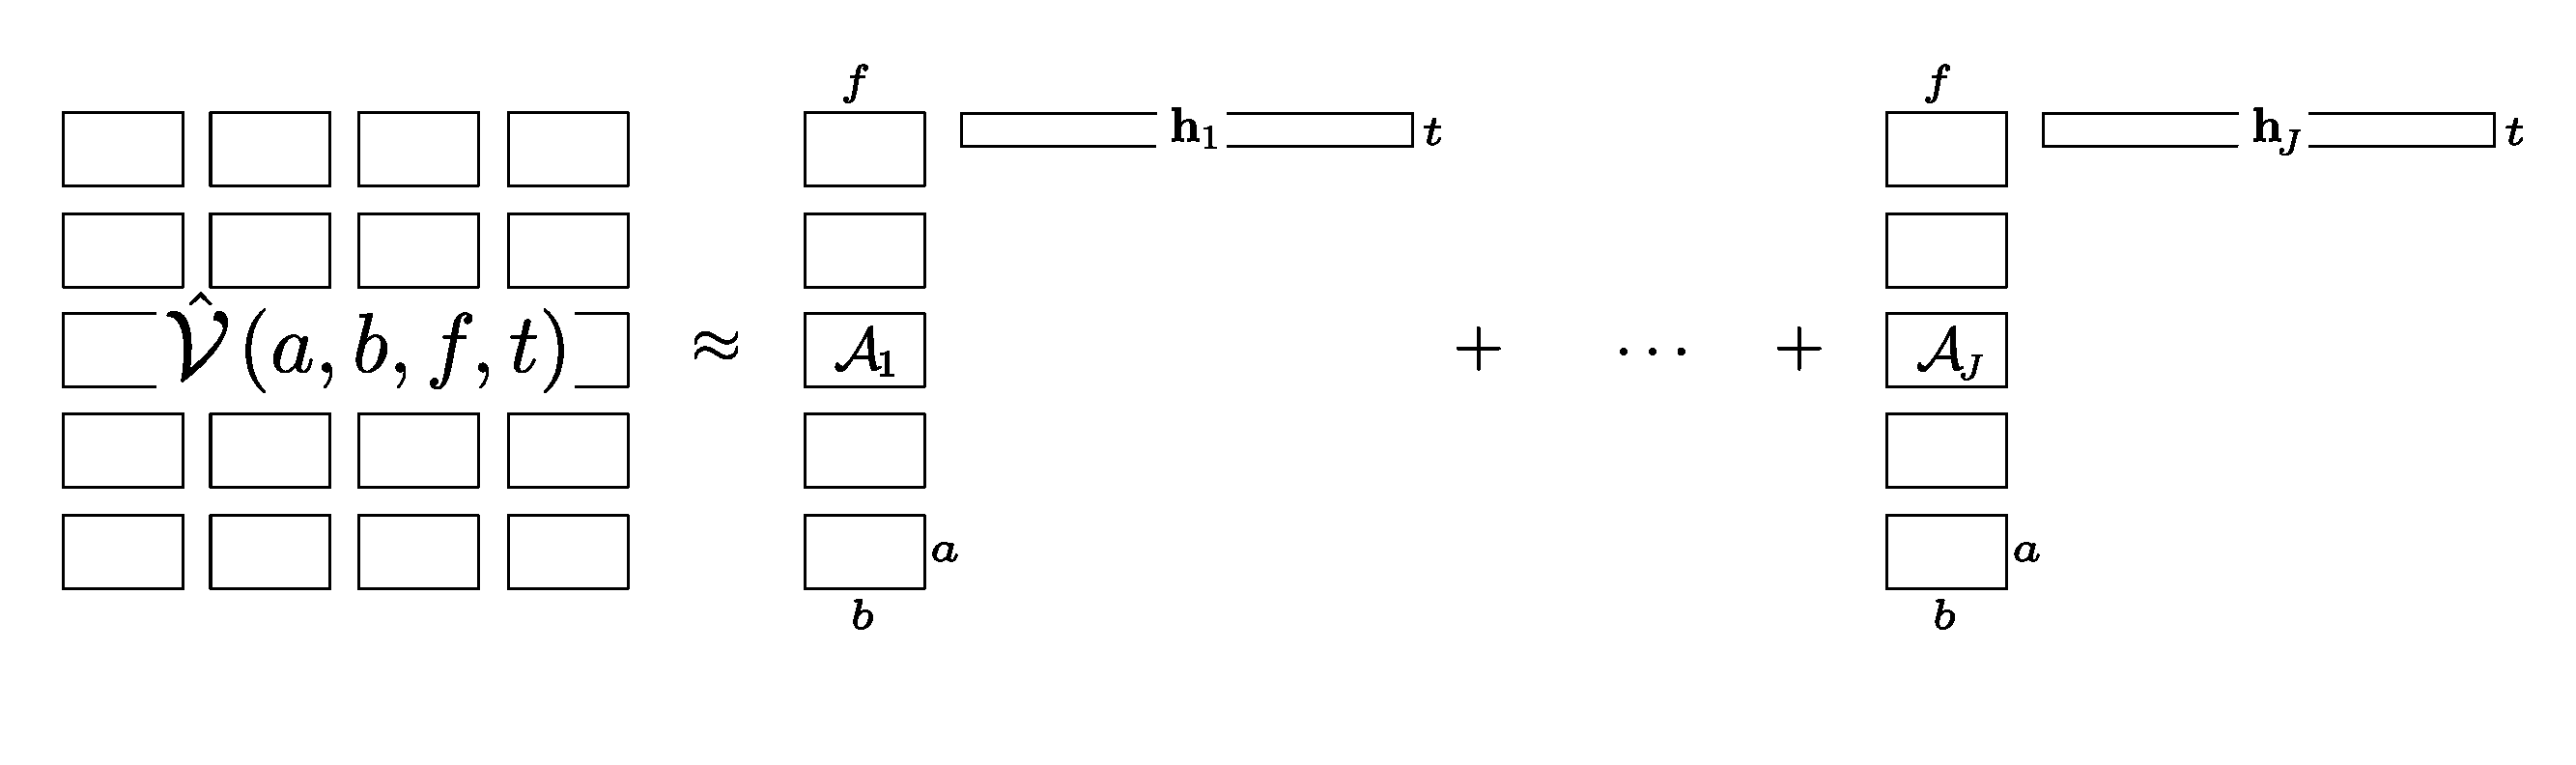
\includegraphics[width=0.9\columnwidth]{Chapters/06_Separation_Unknown/figures/cfm.pdf}
\caption{Visualization of the Common Fate factorization model (CFM).}
\label{fig:cfm}
\end{figure}

Learning those parameters can be achieved using the non-negative
tensor factorization (see e.g.~\cite{cichoki09,ozerov12,smaragdis14}
for an overview), except that it is applied to the CFT instead of the STFT,
and that the particular factorization to be used is~\eqref{eq:NTF_model}.

In essence, it amounts to estimating the parameters~$\{ A_{k},H_{k}\} $
so that the modulus of the CFT is
as close as possible to~$\sum_{k}P_{k}$, with some particular
cost function as a data-fit criterion called a $\beta$-divergence
and which includes Euclidean, Kullback-Leibler and Itakura-Saito as
special cases~\cite{fitzgerald08a}. As usual in non-negative models,
each parameter is updated in turn, while the others are kept fixed.
We provide the multiplicative updates in Algorithm~\ref{alg:Fitting-NTF}.
After a few iterations, the parameters can be used to separate the sources using the Wiener filter as described in~\cite{liutkus15}.

\begin{algorithm}
With $v=\left|x\right| \forall a,b,f,t v(a,b,f,t) = |x(a,b,f,t)|$ and always using the latest
parameters available for computing
 $\hat{P}\left(a,b,f,t\right)=\sum\limits_{k=1}^{K}A_{k}\left(a,b,f\right)H_{k}\left(t\right)$,
iterate:
\[
A_{k}\left(a,b,f\right)\leftarrow A_{k}\left(a,b,f\right)\tfrac{\sum_{t}v\left(a,b,f,t\right)\hat{P}\left(a,b,f,t\right)^{\cdot\left(\beta-2\right)}H_{k}\left(t\right)}{\sum_{t}\hat{P}\left(a,b,f,t\right)^{\cdot\left(\beta-1\right)}H_{k}\left(t\right)}
\]
\[
H_{k}\left(t\right)\leftarrow H_{k}\left(t\right)\tfrac{\sum_{a,b,f}v\left(a,b,f,t\right)\hat{P}\left(a,b,f,t\right)^{\cdot\left(\beta-2\right)}A_{k}\left(a,b,f\right)}{\sum_{a,b,f}\hat{P}\left(a,b,f,t\right)^{\cdot\left(\beta-1\right)}A_{k}\left(a,b,f\right)}.
\]

\caption{Fitting parameters of the non-negative CFM~\eqref{eq:NTF_model}.\label{alg:Fitting-NTF}}
\end{algorithm}

%!TEX root = ../icassp2016.tex
\subsection{Experiments}
\label{sec:experiment}

In this section, we present separation experiments utilizing CFM and compare it with other methods.

\begin{table*}[ht!]
  \centering
  \scriptsize
\begin{tabular}{ llll }
    \toprule
    Method & Signal Representation & Factorization Model \\
    \midrule
    CFM~\cite{stoter16} & STFT $\rightarrow$ Grid Slicing $\rightarrow$ 2D-DFT & $V(a,b,f,t) = P(a,b,f)\times H(t)$ \\
    NMF~\cite{virtanen07} & STFT & $V(f,t) = W(f)\times H(t)$ \\
    HR-NMF~\cite{badeau13} & Output of any filterbank (STFT, MDCT, \ldots)  & AR filtering of NMF excitation \\
    MOD~\cite{barker13} & STFT $\rightarrow$ $|\ldots|$ $\rightarrow$ STFT along each bin & $V(f,m,t) = W(f)\times A(m)\times H(t)$ \\
    CFMM & STFT $\rightarrow$ $|\ldots|$ $\rightarrow$ Grid Slicing $\rightarrow$ 2D-DFT & $V(a,b,f,t) = P(a,b,f)\cdot H(t)$ \\
    CFMMOD & STFT $\rightarrow$ $|\ldots|$ $\rightarrow$ Grid Slicing $\rightarrow$ 2D-DFT & $V(a,b,f,t) = P(a,b,f)\cdot H(t)$ \\
    \bottomrule
\end{tabular}
\caption{Overview of the evaluated algorithms.}
\label{tab:methods}
\end{table*}

\subsubsection{Synthetic Example}
\label{sub:Synthentic_Examples}

To illustrate the CFT representation, we processed a mixture consisting of two sinusoidal sources. One source is a pure sine wave of fundamental frequency 440~Hz whereas the other is frequency modulated by a sinusoid of 6.3~Hz. In the first step, an STFT with a DFT-length of 1024 samples and a hop-size of 256 samples were processed at a sample rate of 22.05~kHz. Patches of size $(N_a, N_b) = (32, 48)$ (not respecting overlaps) were then taken from the STFT output. Figure~\ref{fig:CFT} in Section~\ref{sub:CFT} then shows the Common Fate Transform for the mixture. One can see that the CFT representation shows distinct patterns across time, suggesting that the factorization is able to separate the sources. 
Furthermore, if we now looking at a smaller excerpt of the same synthetic example, depicted in Figure~\ref{fig:gridplot}, we can also observe the additivity property of the common fate representations.

\begin{figure}[!h]
\centering
        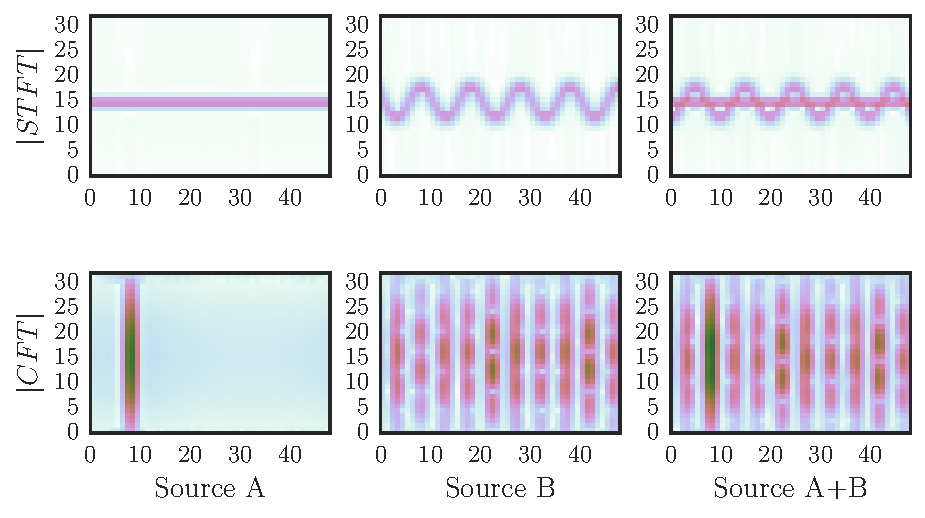
\includegraphics[width=0.9\textwidth]{Chapters/06_Separation_Unknown/figures/gridplot.pdf}
\caption{Examples of patches of size $(N_a, N_b) = (32, 48)$. The upper row shows the STFT output, the lower row the corresponding Common Fate Transform (CFT). \textsuperscript{\textregistered}2016 IEEE.}
\label{fig:gridplot}
\end{figure}

\subsubsection{Objective Evaluation on Unison Instrument Mixtures}

To evaluate the proposed method, five musical instrument samples were selected from the Unison Separation Dataset~\cite{oss_unison} --- all of them feature vibrato: violin, cello, tenor sax, English horn, and flute. It is important to note that vibrato techniques differ between these instruments: whereas the English horn and the flute only produce a very subtle modulation, the violin and tenor sax have powerful frequency modulations with a higher modulation frequency as well as a higher modulation index. 
All samples last about three seconds. 
We then generated a combination of ten mixtures of two instruments, each one generated with a simple SourceA --- SourceB --- (SourceA + SourceB) scheme. Data were encoded in 44.1 kHz / 16 bit.
We compared the separation performance of six different methods, summarized in Table~\ref{tab:methods}:
\begin{description}[style=unboxed,leftmargin=0cm]
\item[CFM] For the CFM model, we took an STFT with frames of 1024 samples and a hop-size of 512 samples. The resulting complex STFT was then split into a grid of patches of size $(N_a, N_b) = (4, 64)$, each having a half-window overlap in both dimensions.
\item[MOD] We implemented a modified version of~\cite{barker13} where for the sake of comparability, we used a STFT instead of a gammatone filterbank. A DFT length of 1024 and a hop-size of 512 samples were chosen. After taking the magnitude value, a second STFT of size 32 and hop-size 16 samples was computed for each frequency.
\item[CFMMOD] We selected patch sizes of $(N_a, N_b) = (1, 64)$ and modified the representation so that the magnitude was applied before computing the 2D-DFT.\@ This permits to compare the advantage of our proposed factorization model~(\ref{eq:NTF_model}) over MOD, when using the same kind of energy-modulation representation in both cases.
\item[CFMM] For comparing the influence of computing modulations over complex STFT or magnitude STFT, we tried our factorization model when the magnitude of the STFT is taken before 2D-DFT, with patches of the same size as for the CFM method.
\item[NMF] We took a ``standard'' NMF based method~\cite{virtanen07}. We highlight that taking a STFT with frames of length 1024 would not make a fair comparison, because the CFM model actually results in a larger frequency resolution. Therefore a comparable NMF is based on an STFT of DFT-length 32768.
\item[HR-NMF] See description in~\cite{magron15a}.
\end{description}
All factorizations ran for 100 iterations and were repeated five times. We chose $k=(2,\ldots,6)$ components for each factorization. For $k > 2$ we used oracle clustering to show the upper limit of SDR which can be achieved.

We ran the performance evaluation by using BSSeval~\cite{vincent06}. The results of Signal to Distortion
Ratio (SDR), Signal to Interference Ratio (SIR), and Signal to Artifacts Ration (SAR) are depicted in Figure~\ref{fig:boxplot_overall}. 
Results indicate that the CFM model performs well in all measures. 
However, in terms of SIR, the results of HR-NMF are better than CFM method. The results for CFMMOD and CFMM indicate the positive influence of the CFM factorization compared to~\cite{barker13}.
The results of CFMM indicate that the complex CFT lead to better results. NMF did perform surprisingly well, which may only hold for our test set, where each source is active for a long period. This results in a cyclic stationary vibrato, revealing spectral side lobes at such a high resolution. With more than one component per source, the results of CFM do improve, but it can be seen that more than two components ($k=4$) will not increase the SDR values. The separation results and a full Python implementation of the CFM algorithm can be found on the companion website~\footnote{\url{github.com/aliutkus/commonfate}}.

\begin{figure}[ht!]
\centering
        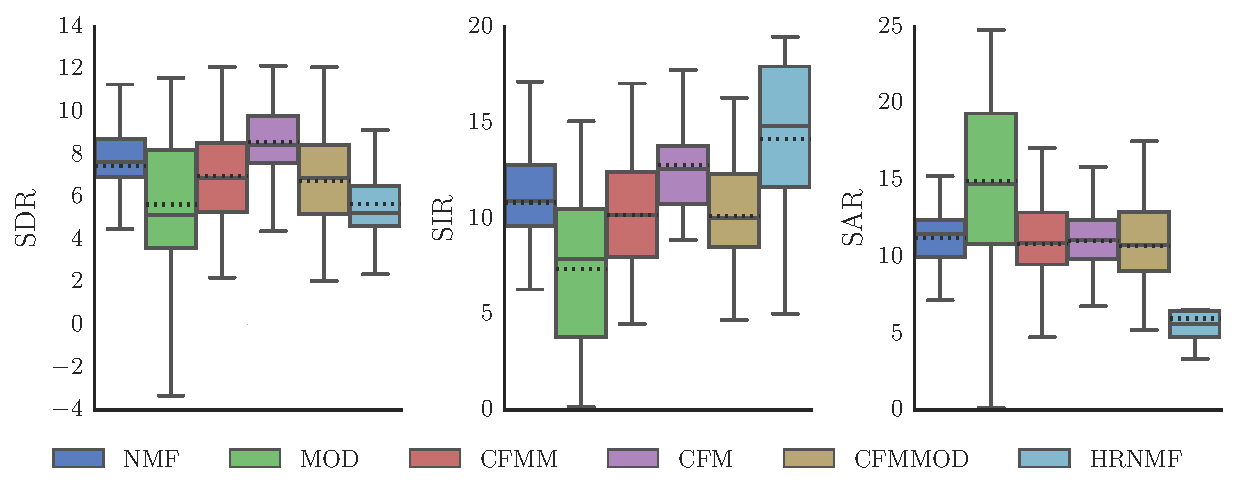
\includegraphics[width=0.8\textwidth]{Chapters/06_Separation_Unknown/figures/cfm_boxplot.pdf}
\caption{Boxplots of BSS-Eval results of the unison dataset. Solid/dotted lines represent medians/means. \textsuperscript{\textregistered}2016 IEEE.}
\label{fig:boxplot_overall}
\end{figure}

\begin{figure}[ht!]
\centering
        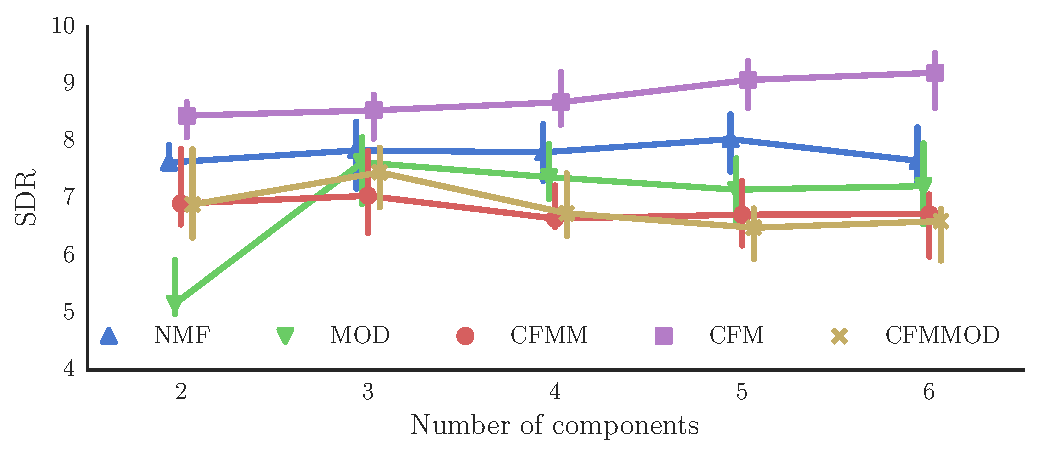
\includegraphics[width=0.8\textwidth]{Chapters/06_Separation_Unknown/figures/iterations.pdf}
\caption{Boxplots of SDR values of the unison dataset over the number of components $k$. For $k>2$ oracle clustering was applied. \textsuperscript{\textregistered}2016 IEEE.}
\label{fig:iterations}
\end{figure}

\section{Common Fate Transform for Music Separation}%
\label{sec:cft_for_lead_accompaniment_separation}

In the previous section, we showed that the Common Fate Model is suitable to separate highly overlapped signals based on their spatial-temporal modulation texture.
In this section, we want to show how this method can be extended for the application of vocal and accompaniment separation~\cite{rafii}.
This scenario is significantly more complex than the separation of instrument mixtures, hence the separation model needs to be flexible enough to handle many of the critical edge cases which make music separation challenging.
With the recent success of machine learning models~\cite{HintonSpeech}, it became likely that an unsupervised model such as NTF or CFM may not be flexible enough to enforce the significant amount of domain knowledge that is present in this scenario to improve performance.
% from zafar
Rafii et. al describe the current machine learning situation in \cite{rafii}:

\begin{quote}
``Taking advantage of the recent availability of sufficiently large databases of isolated vocals along with their accompaniment, several researchers investigated the use of machine learning methods to directly estimate a mapping between the mixture and the sources~\cite{huang14, uhlich15}.
However, most systems today still use classical time-frequency representations.

The common structure of deep learning methods for lead and accompaniment separation usually corresponds to the one depicted in Figure~\ref{fig:methods_dnn}.
Most methods mainly differ in the architecture picked for the network, its input, and output representation as well as in the way the network is trained.

\begin{figure}
  \centering
  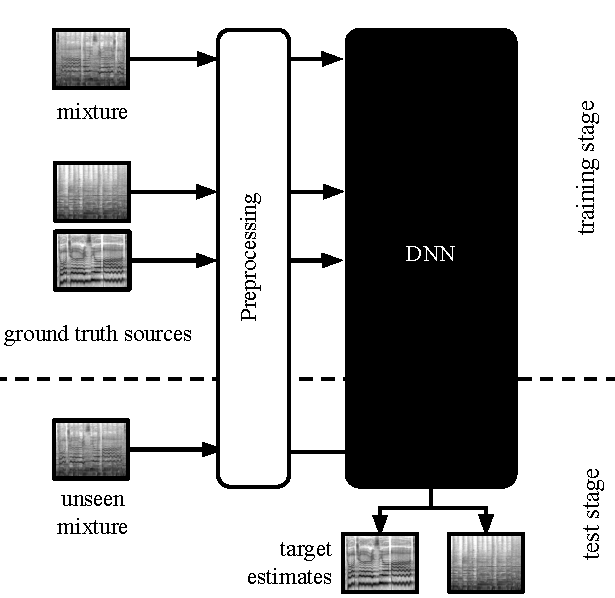
\includegraphics[width=0.6\textwidth]{Chapters/06_Separation_Unknown/figures/methods_dnn.pdf}
  \caption{General architecture for methods exploiting deep learning. The network inputs the mixture and outputs either the sources magnitude STFT or a TF mask. Methods usually differ in their network architecture and the way use the training data for learning (a different version of this Figure was published in~\cite{rafii}). \textsuperscript{\textregistered}2018 IEEE.}
  \label{fig:methods_dnn}
\end{figure}

% from zafar
For the understanding of this section, it is sufficient to mention that DNNs consist of a cascade of several, possibly non-linear transformations of the input, which are learned during a training stage.
They were shown to effectively learn representations and mappings, provided, enough data is available for estimating their parameters \cite{deng14, lecun15, goodfellow16}.
Different architectures for neural networks may be combined/cascaded together, and many architectures were proposed in the past, such as fully-connected neural networks (FNN), convolutional neural networks (CNN), or recurrent neural networks (RNN) and variants thereof such as the long short-term memory (LSTM) and the gated-recurrent units (GRU).
Training of such functions is achieved by stochastic gradient descent \cite{robbins51} and associated algorithms, such as backpropagation~\cite{rumelhart862} or backpropagation through time~\cite{rumelhart86} (BTT) for the case of RNNs.
\par
%The first one: Huang
% zafar
Huang et al. were the first to propose RNNs~\cite{hermans13,pascanu14} for singing voice separation in \cite{huang14,huang15}. They adapted their framework from \cite{huang142} to model all sources simultaneously through masking. Input and target functions were the mixture magnitude and a joint representation of the individual sources. The objective was to estimate jointly either singing voice and accompaniment music, or speech and background noise from the corresponding mixtures.
\par
%Exploiting context: FNN with context, LSTM
Modeling the temporal structures of both the lead and the accompaniment is a considerable challenge. As an alternative to the RNN approach proposed by Huang et al. in \cite{huang14}, Uhlich et al. proposed the usage of simpler FNNs \cite{uhlich15} whose input consists of \textit{supervectors} stacked of few consecutive frames from the mixture.''
\end{quote}
We decided to reimplement Uhlich's model~\cite{uhlich15} to evaluate the separation quality.
The aim of this work was not to exactly reproduce the results, but instead, to evaluate one main research questions: does a DNN-based model benefit from the common fate representation being able to better capture the modulation texture?
For the implementation of the model, we used the Keras~\cite{chollet15} deep learning framework to systematically assess different combinations of input-and-output representation of the system.

\par
The network, as proposed in~\cite{uhlich15} consists of a three-layer fully connected network, where each of the hidden layers has the same number of hidden nodes as the targeted output representation.
This method can be described as a variant of a stacked denoising autoencoder~\cite{pvincent08}, where the noisy input is mapped to a clean output of the same dimensionality.
The architecture is depicted in Figure~\ref{fig:cft_dnn}. 

\begin{figure}[ht!]
\centering
        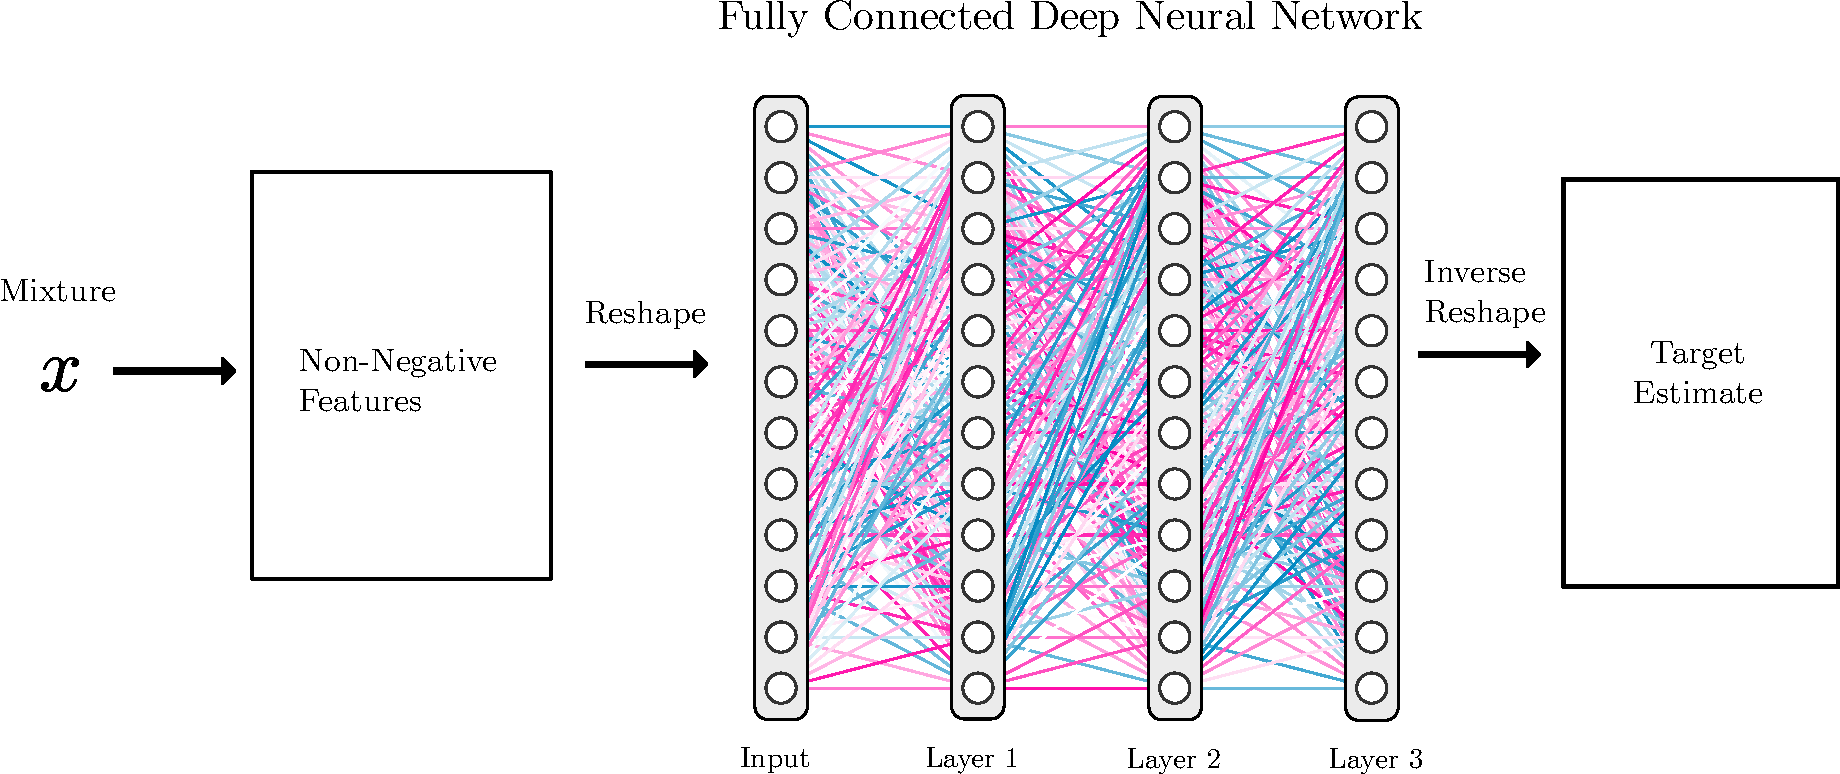
\includegraphics[width=\textwidth]{Chapters/06_Separation_Unknown/figures/uhlich_dnn.pdf}
\caption{Simplified block diagram of fully connected denoising autoencoder network as proposed by~\cite{uhlich15} for time-frequency based separation.}
\label{fig:cft_dnn}
\end{figure}

\subsection{Inputs and Outputs}

The purpose of the model is to create a non-linear mapping function from the magnitude of the input mixture \(\mX\) to the magnitude of the target source \(\mY_j\).
The optimal parameters (weights) \(\theta_j\) of such a mapping function \(\mY_j = f_{\theta_j}(\mX)\) are learned via supervised training.
FNN networks, such as the one used here, can only deal with temporal structure by reshaping the time-frequency input to a super vector to be processed by the FNN. 
However, this drawback is compensated by a large number of parameters in an FNN layer.

Since the STFT, GFT and CFT are lapped transforms, different scenarios for the input and output representation of the FNN can be envisioned:

\begin{description}[style=unboxed,leftmargin=0cm]
\item[STFT-STFT]: for the \emph{input}, we computed the STFT (\(N=1024, Hop=512\) of each the audio track and select excerpts of size, \(\mathbf{X} \in \mathcal{R}^{2C + 1}_{+} \), where \(C\) is the number of preceding and succeeding frames around the central frame \(\mathbf{X}_{i+C}\). For the \emph{output}, only a single central frame \(\mathbf{Y}_{i+C}\) is selected.
We used \(C=2\), reflecting the setting in~\cite{uhlich15}. This results in an input sample size of \(\mathbf{X} \in \mathcal{R}_{+}^{5 \times 513}\) and  \(\mathbf{Y} \in \mathcal{R}_{+}^{1 \times 513}\).

\item[GFT-GFT/GFT-STFT]: instead of taking excerpts from the STFT, like in \emph{STFT-STFT}, we computed overlapping patches, as described in Section~\ref{sub:CFT}. Each patch is of size \((5, 8)\), which means that the same number of time frames are used compared to \emph{STFT-STFT} but additional redundancy has been added because of the overlap between neighboring patches.
For the \emph{output}, we chose the GFT of \(Y\).
This results in an input sample size of \(\mathbf{X} \in \mathcal{R}_{+}^{128 \times 5 \times 8}\) and  \(\mathbf{Y} \in \mathcal{R}_{+}^{128 \times 5 \times 8}\).
Furthermore, to reduce the number of parameters, we also evaluated a setting where just the \emph{output} is the central frame of the STFT.

\item[CFT-CFT/CFT-STFT]: in the first step, a processing as in \emph{GFT-GFT} was applied and then the 2D-DFT transform was applied (see Section~\ref{sub:CFT}).
The results in identical shapes as in the \emph{GFT-GFT} but with added benefits of this representation that can model neighboring phase dependencies.
\end{description}

We used the DSD100 dataset~\cite{ono15} for training and test. 
For each sample fed into the network, we randomly selected mixtures (without replacement) from the DSD100 dataset.

\subsection{Training}
We then sample from the DSD100 tracks and form single samples as input for the FNN.
Therefore, we first compute the input representation of an audio track from the DSD100 set and then randomly sampling without replacement from these tracks.
The actual training has been done using mini-batches of size 32.
Each architecture is trained using the ADAM optimizer~\cite{kingma14} (learning rate: \(1 \cdot 10^{-3}\), \(\beta_1=0.9\), \(\beta_2=0.999\), \(\epsilon=1 \cdot 10^{-8}\))
The model was trained for a fixed number of 30 epochs and, in contrast to~\cite{uhlich15}, greedy layerwise pre-training was not applied.

\subsection{Results}

\begin{figure}[t]
\centering
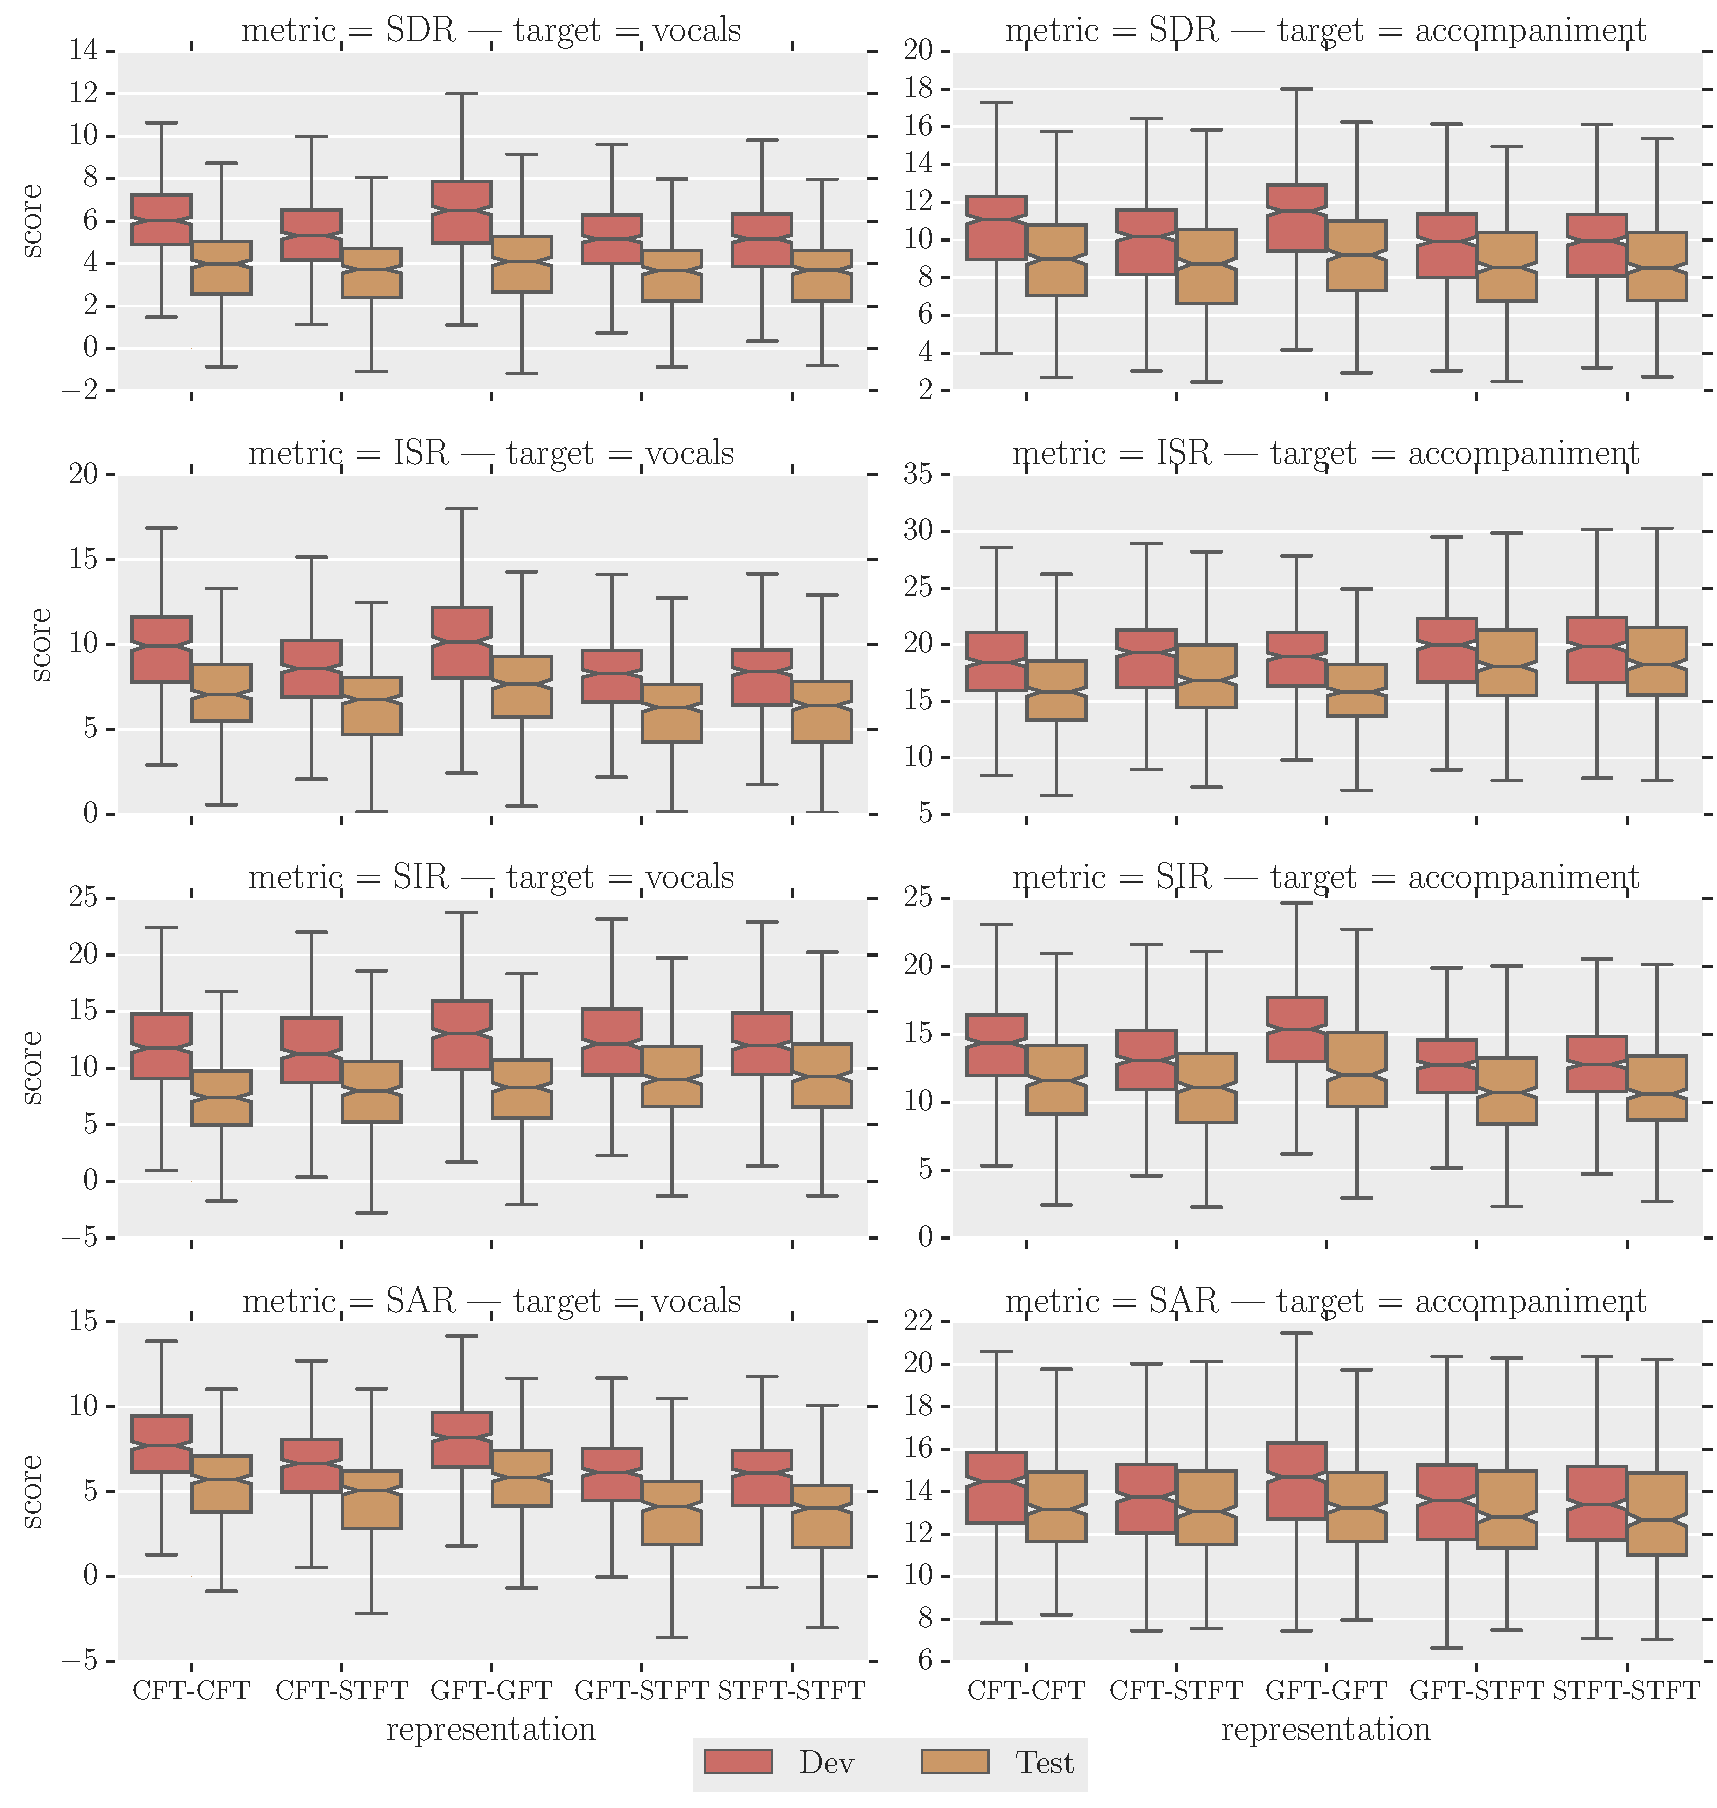
\includegraphics[width=1.1\textwidth]{Chapters/06_Separation_Unknown/figures/boxplot.pdf}
\caption{BSSEval separation results of the DSD100 dataset results for vocals and accompaniment sources. Several combinations of `input-output` were tested, as indicated by the x-axis.}
\label{fig:deep_cft_boxplots}
\end{figure}

For evaluation, the BSSEval metrics of all representations for the DSD100 test set were computed.
The results are depicted in Figure~\ref{fig:deep_cft_boxplots}.
They indicate that the common fate representation is indeed improving the baseline \emph{STFT-STFT} results.
Overall, we can report a mean difference of 0.4~dB for CFT-CFT and 0.5dB for GFT-GFT, compared to the \emph{STFT-STFT} representation.
However, it is worth mentioning that both, the GFT and the CFT representation lead to a significant increase in redundancy in the representation, thus increasing the number of trainable parameters per network layer (26 million for CFT vs 0.26 million for STFT). Since we could not observe a large increase in difference of training (Dev) vs. test (Test) performance, we assume that the increasing number of parameters do not lead to large overfitting.

\subsection{Submission to SiSEC 2016}
\label{ssec:performance}

The results have been submitted to the 2016 SiSEC source separation challenge~\cite{sisec16}.
This enables to relate the work compared to $22$ other source separation methods, all evaluated on the same test data, as part of the task for separating professionally-produced music recordings at SiSEC 2016.
Table~\ref{tab:sisec_systems} lists the participating systems.
\begin{table*}[htbp]
  \centering
  \scriptsize
    \begin{tabular}{lll@{}}
        \hline
        \textbf{Acronym} & \textbf{Ref.} & \textbf{Summary}\\
        \hline
        STO1 & Proposed & FNN on GFT representation \\
        STO2 & Proposed & FNN on CFT representation \\
        HUA & \cite{huang12} & RPCA standard version \\
        RAF1 & \cite{rafii13} & REPET standard version \\
        RAF2 & \cite{liutkus12} & REPET with time-varying period \\
        RAF3 & \cite{rafii12} & REPET with similarity matrix \\
        KAM1-2 & \cite{liutkus15} & KAM with different configurations \\
        CHA & \cite{chan15} & RPCA with vocal activation information \\
        JEO1-2 & \cite{jeong17} &  $l_1$-RPCA with vocal activation information \\
        DUR & \cite{durrieu11} & Source-filter NMF \\
        OZE & \cite{salaun14} & Structured NMF with learned dictionaries \\
        KON & \cite{huang15} & RNN \\
        GRA2-3 & \cite{grais16} & DNN ensemble \\
        UHL1 & \cite{uhlich15} & FNN with context \\
        NUG1-4 & \cite{nugraha16} & FNN with multichannel information \\
        UHL2-3 & \cite{uhlich17} & LSTM with multichannel information \\
        IBM & & ideal binary mask \\
  \end{tabular}
     \caption{Methods evaluated in SiSEC 2016.}
    \label{tab:sisec_systems}

\end{table*}

%announcing the results and the webpage
The objective scores for my proposed methods were obtained using BSSEval and are given in Figure~\ref{fig:eval}.

\begin{figure*}[htbp]
    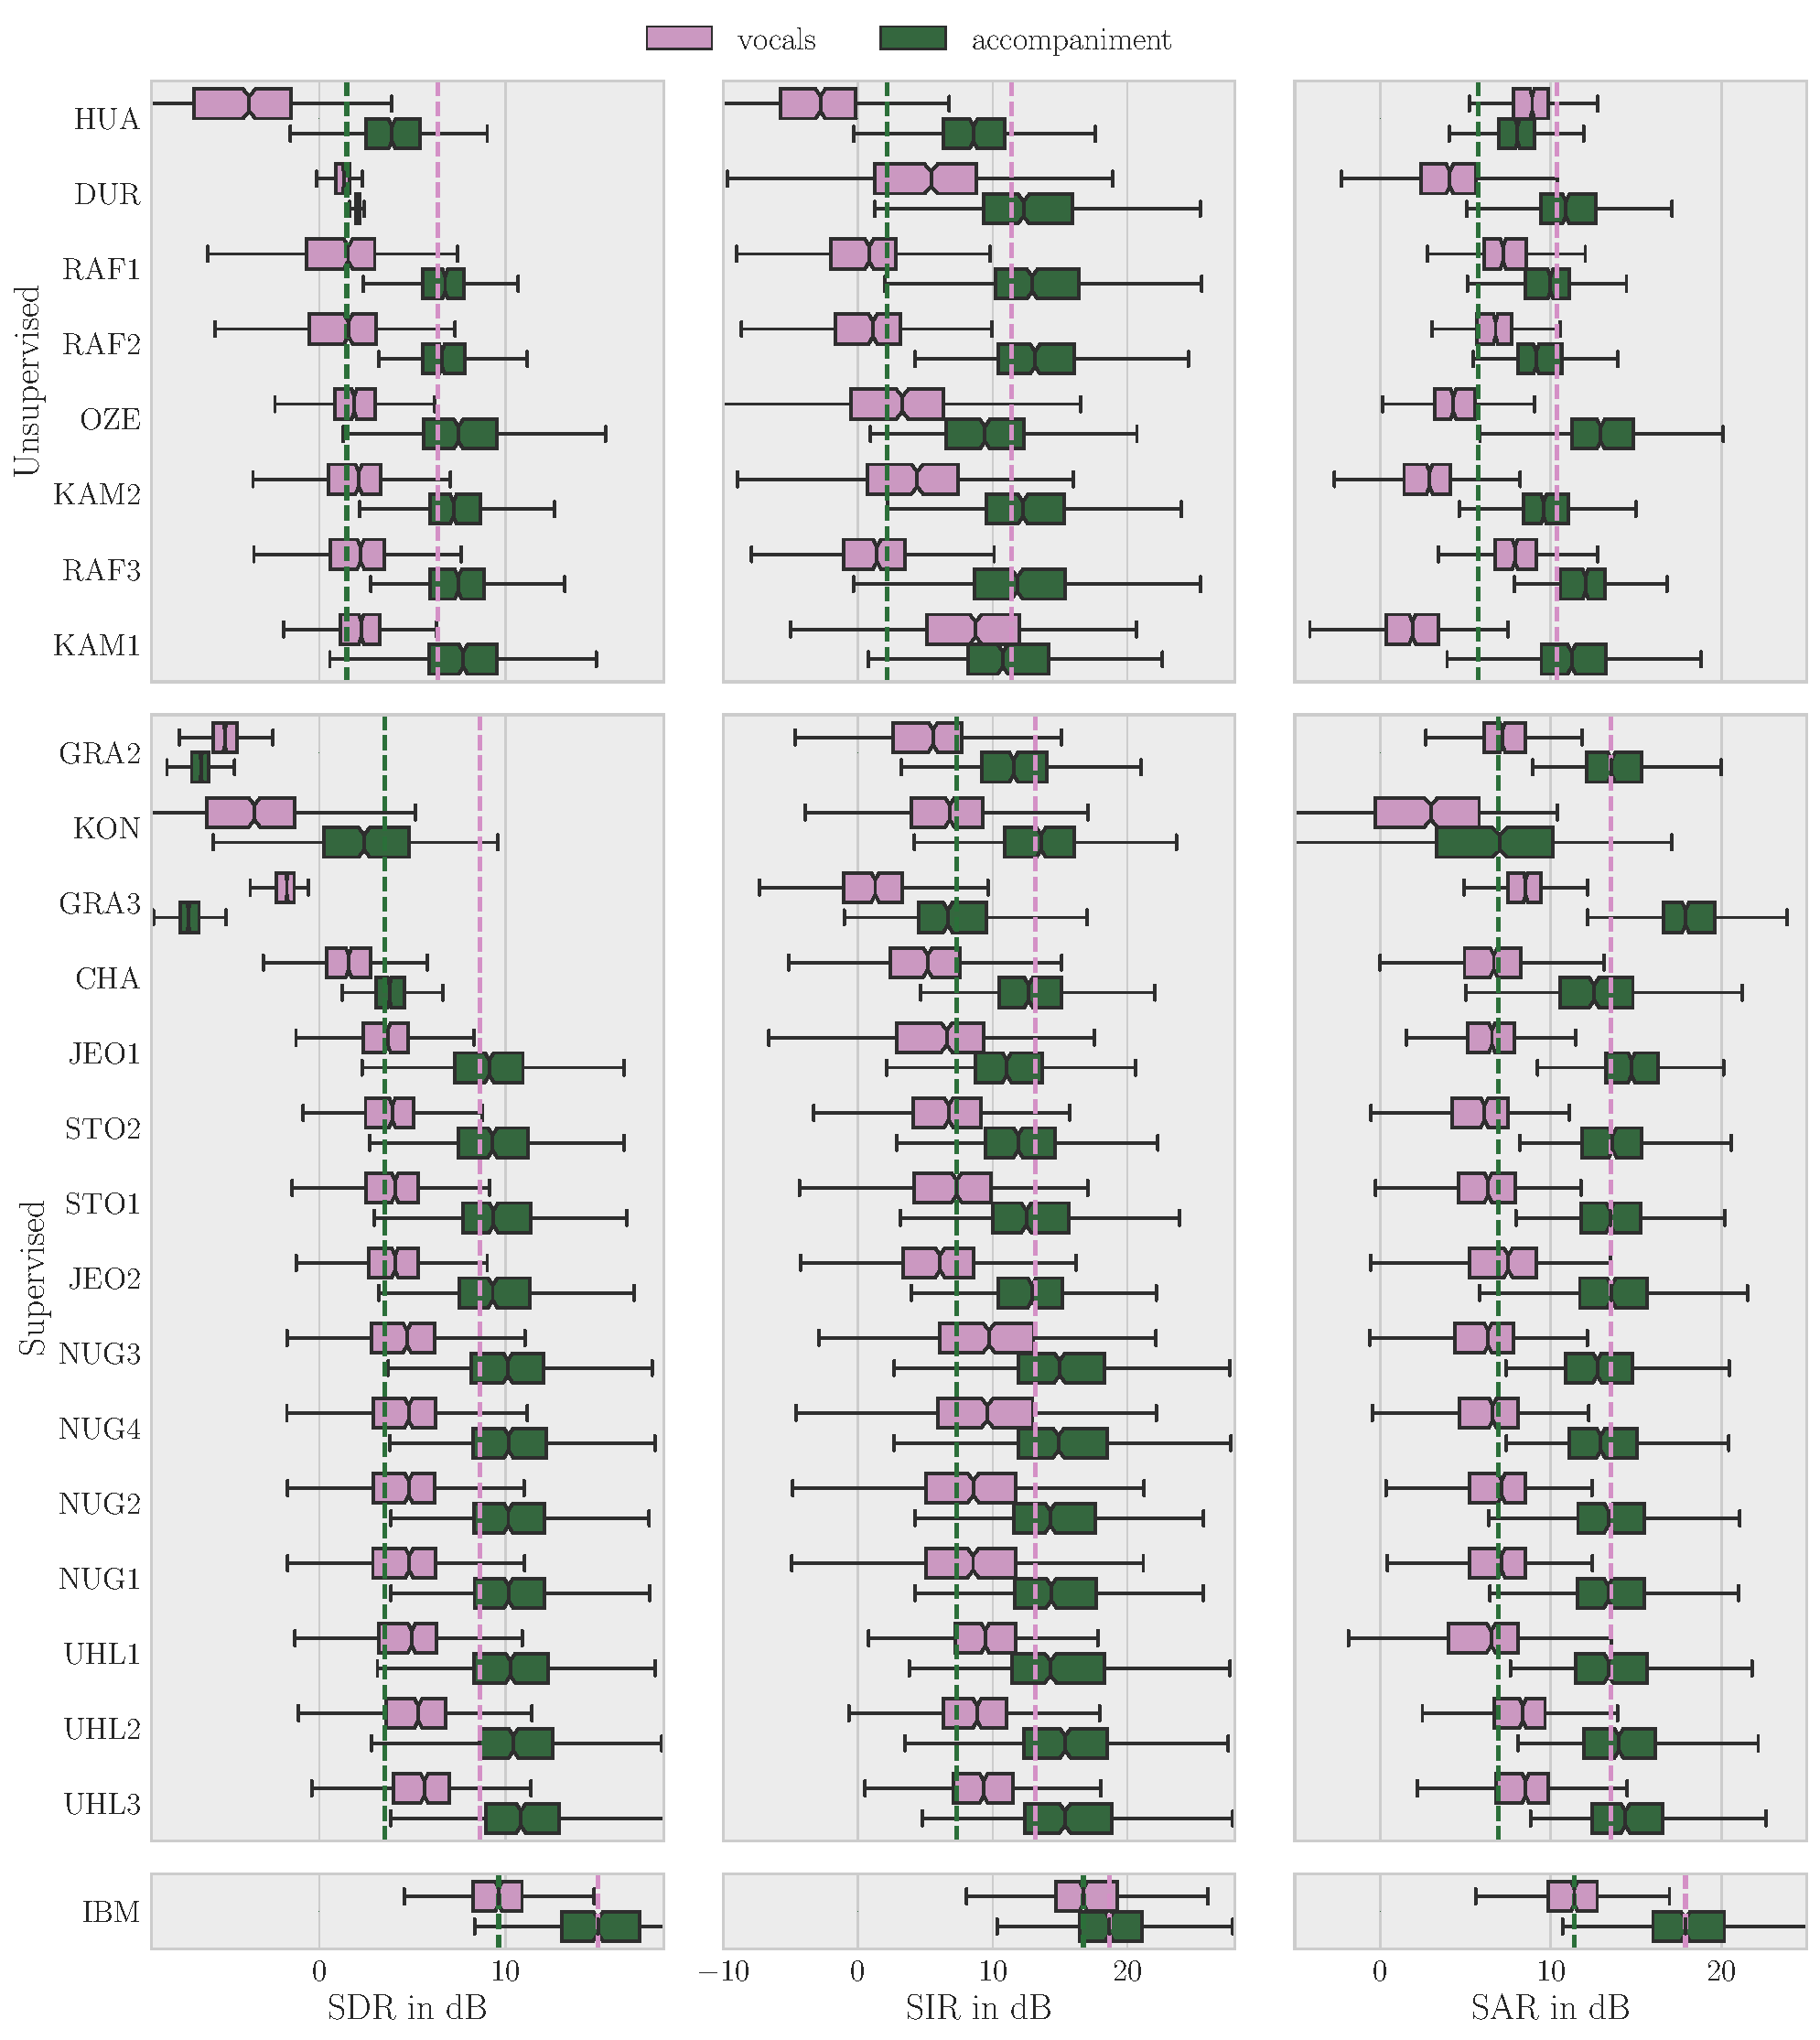
\includegraphics[width=1.1\textwidth]{Chapters/06_Separation_Unknown/figures/evaluation.pdf}
    \caption{BSSEval scores for the vocals and accompaniment estimates for SiSEC 2016 on the DSD100 dataset. Results are for both test set (Test) as well as the training dataset (Dev). Scores are sorted according the vocal median SDR and grouped by supervised and unsupervised methods. The proposed systems are \emph{STO1}, based on GFT-GFT and \emph{STO2}, based on CFT-CFT.}
    \label{fig:eval}
\end{figure*}

% Maybe want to rewrite as it has been stolen from zafar
An obvious observation in Figure~\ref{fig:eval} is the difference in performance between data-driven methods and ``classical'' unsupervised methods. 
Further, it shows that exploiting learning data does help separation compared to only relying on \textit{a priori} assumptions such as the harmonicity or redundancy. Additionally, dynamic models such as LSTM from UHL2-3 appear more adapted to music than FNN. 
These good performances in audio source separation go in line with the success of DNNs in fields as varied as computer vision, speech recognition, and natural language processing \cite{lecun15}.
\par
Relating our results of STO1 and STO2 to the other methods, we observe that the performance was only slightly below the two state-of-the-art performance of UHL and NUG.
Furthermore, the difference between test and validation dataset indicate, that our CFT DNN model even has better generalization as the one in NUG. 
While our STO model share the same network architecture as UHL1, we were unable to reproduce the results, as we are approximately 1~dB below UHL1.
One reason is in the difference in initialization of the model as well as the fact that NUG and UHL models exploit multichannel information. 

\subsection{Evaluation Website}
\label{ssec:evaluation Website}

For more details and the ability for playback of the estimates, we refer to the dedicated interactive website that we built as part of my organizational help for SiSEC\footnote{\url{http://www.sisec17.audiolabs-erlangen.de}}.
In fact, for the first time, interested researchers are now able to listen to over 10000 stimuli from all participating systems.
This was made possible through modern JavaScript technologies like the Web Audio API to interactively assess source separation results in the browser.
For each track, separation results are provided as well as the objective BSSeval scores, all of the data is reproducible and was made available in~\cite{oss_sisecwebsite}.
Figure~\ref{fig:sisec_website} depicts a screenshot of the website.
The objective scores are depicted as an interactive matrix where users are able to sort the results for each track and each system interactively by the source of interest.
Clicking on one rectangle in the heatmap opens the interactive player that allows to simultaneously playback the separated sources including changing the volume of each source.

\begin{figure}[!h]
\centering
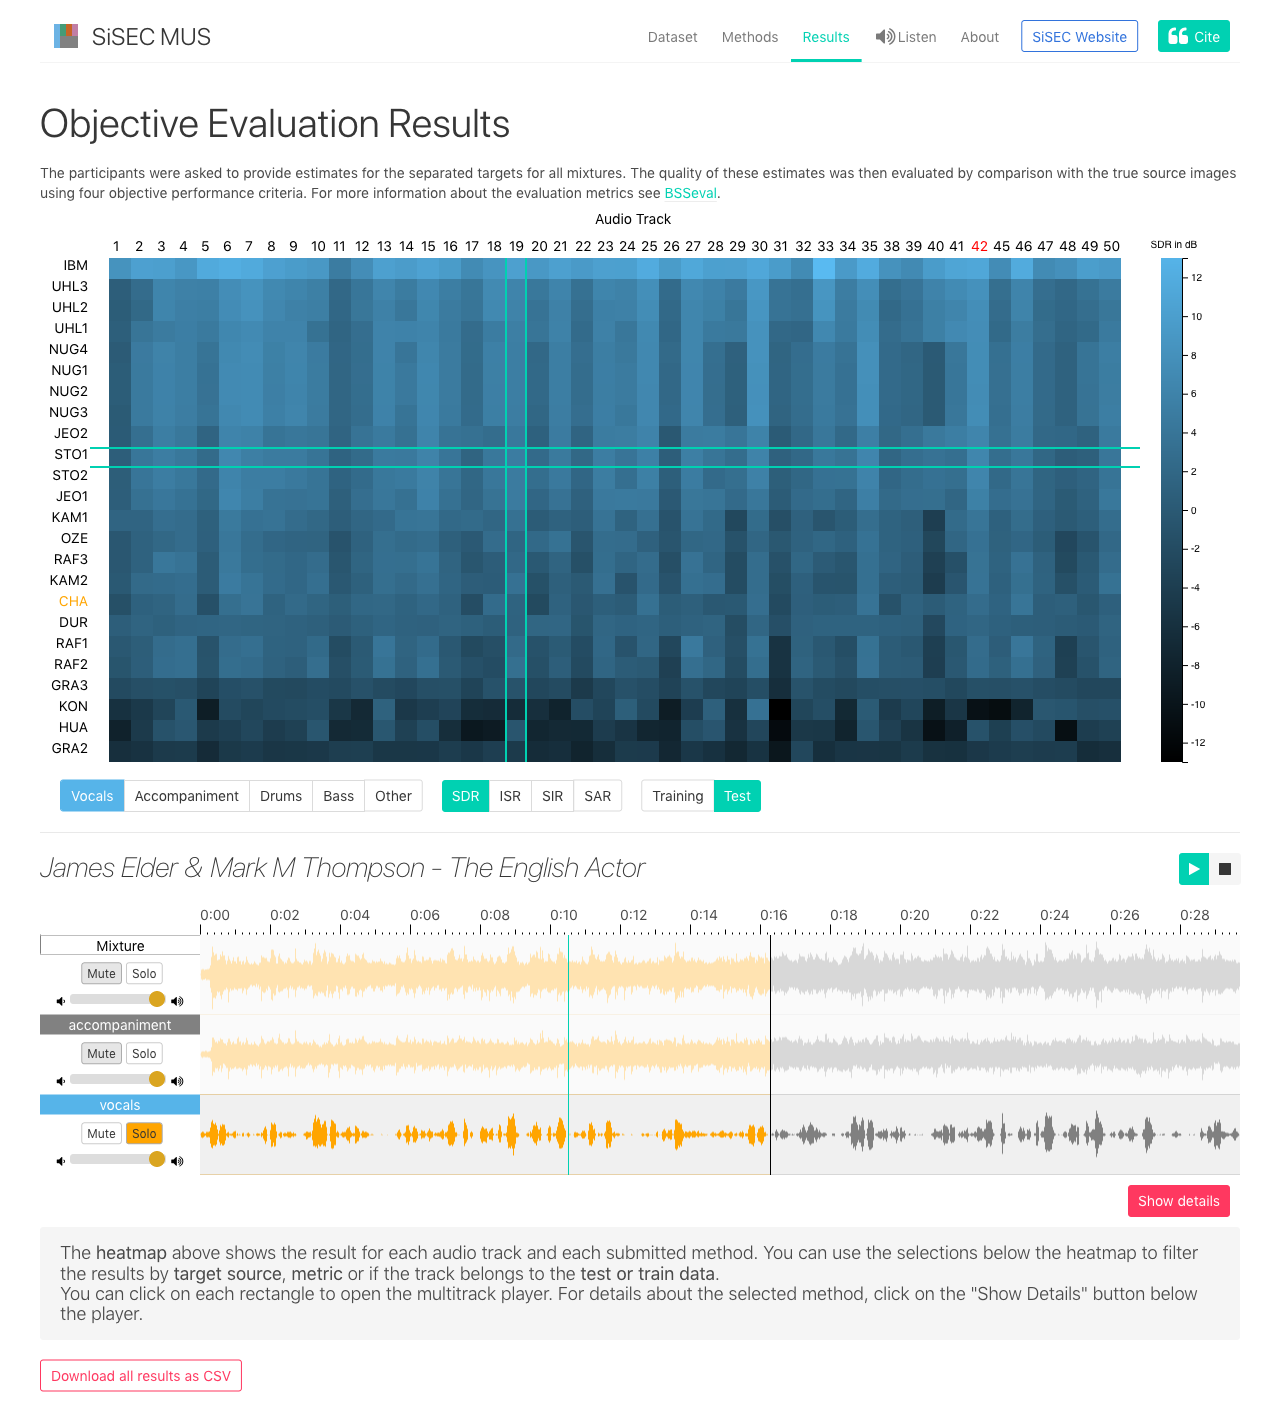
\includegraphics[width=0.9\textwidth]{Chapters/06_Separation_Unknown/figures/sisec_website.png}
\caption{Screenshot of the SiSEC 2016 Website~\url{http://sisec17.audiolabs-erlangen.de}}
\label{fig:sisec_website}

\end{figure}

\section{Summary and Discussion}

In this chapter, we presented methods that exploit modulations for source separation without knowing them a priori. 
In the first part of this chapter, we presented a study where we demonstrated the use of the modulation spectrogram tensors for separating unison instrument mixtures, comparing the results with those presented in the previous chapter.
In a next step, we proposed a complex tensor representation, the Common Fate Transform (CFT), computed from rectangular patches of the complex STFT using two-dimensional DFTs.
This novel representation exposes joint modulation characteristics of amplitude and frequency modulated signals while being fully invertible.
We demonstrated the usefulness of this representation using our Common Fate Model that factorizes patches from the CFT into two components, a modulation pattern and its activation. 
The model is inspired by the human's ability to group common modulations into single sources.
We presented results on unison musical instrument mixtures, indicating that it outperforms existing methods.
\par
In the second part of this chapter, we combined the CFT with an existing deep learning based separation model~\cite{uhlich15}.
We showed that the CFT improved separation quality compared to STFT in a fully connected deep neural network.
Even though the CFT significantly increases the input size (due to its redundancy) and the number of trainable network parameters (due to its stacked auto-encoder architecture), generalization performance did not suffer.
\par
The results of the best performing model were submitted to SiSEC 2016, where we scored among the top three participating research teams.
Finally, we presented interactive evaluation tools, developed for SiSEC, allowing to interactively assess the performance of separation systems both objectively and subjectively.
% \chapter[Experiments on Estimating the Number of Sources]{One, Two, Three, Many: Perceptual Experiments on Estimating the Number of Sources}
\label{cha:countanalysis}
\bigskip
\bigskip
\bigskip
\bigskip
%
The separation of mixtures into its original audio sources, as presented in the previous chapters, is a challenging task.
Furthermore, source separation is difficult to evaluate, and researchers compare to a known reference even though this does not reflect how humans separate mixtures.
It has long been a research topic to answer the question \emph{if} humans can separate, by fully extracting the desired source or if we can focus our attention on one source --- segregate them~\cite{bregman90}.
Moreover, despite recent progress in auditory science~\cite{carlyon04, koelsch05, rabinowitz13}, research still is investigating how separation takes place in the auditory cortex or other parts of the human brain.
One thing, however, we can assess directly is if humans can reliably detect the number of sources in a mixture of several sources.
\par
In order to address this question, it helps to understand how humans infer counts and if our strategy is depending on the count.
When we look at vision, these are questions that have already been discussed over a hundred years ago in scientific research; an early study in the field of psychology of vision was published by Jevons in 1871~\cite{jevons1871}.
Jenvons presented an experiment to quickly infer the number of objects (beans) and came up with the hypothesis that humans can instantly estimate the number of objects without actually counting and therefore identifying them.
Jenvons mentioned in~\cite{jevons1871}:

\begin{quote}
``It is well known that the mind is unable through the eye to estimate any large number of objects without counting them successively. A small number, for instance, three or four, it can certainly comprehend and count by an instantaneous and apparently single act of mental attention.''
\end{quote}

This ``one-two-three-many'' hypothesis was a fundamental observation.
The fact that we can directly infer the numerosity of small numbers of objects, up to about four, is also known as \emph{subitizing}~\cite{kaufman49, burr10}. We refer to this strategy as ``direct count estimation''.
Concerning our hearing, there are indications that the auditory system is capable of subitizing audio sources~\cite{hoopen79}.
And surprisingly, as shown in~\cite{kashino96, kawashima15}, humans share the same limitations of correctly estimate up to three simultaneously active speakers.
\par
In this chapter, we present two experiments contributing to this interesting field of research.
The first experiment (Section~\ref{sec:ismir}) addresses the question if the number of instruments in polyphonic music is subject to the same limitations.
In the second contribution (Section~\ref{sec:count_experiment}) the aim is to verify the findings of an earlier experiment in~\cite{kawashima15} and increase the number of stimuli to be used for comparison of machine learning based count estimations methods

\section{Instrument Count Estimation}%
\label{sec:ismir}

\marginpar{This chapter was previously published in~\cite{stoeter13} and has been revised for this thesis.}

While source separation methods can be objectively evaluated given a true reference, a human versus machine comparison is cumbersome because measuring the human's ability to perform separation is difficult. However, one can easily evaluate if humans can detect the number of sources in a mixture of several sources.
In this Section, we take a first step towards designing an experiment where we focus on polyphonic music of inhomogeneous timbre, where the question is: What is the number of instruments humans can estimate correctly?
Such knowledge can be used in auditory modeling or as a pre-processing step for source separation algorithms.
\par
In previous work, the perception of concurrent sound sources has been analyzed on different scales so far. 
Bregman's and McAdams'~\cite{mcadams89} auditory stream theory can be seen as an analytical way of describing how sound events are perceived by the human auditory system. 
Unfortunately, it is difficult to model professionally produced music by auditory stream models because of its high complexity.
Also, none of these models is motivated to predict the perceived number of musical sources. 
There are indications that for this task, humans tend to fail if more than three sources are present at the same time~\cite{huron89}.
Kashino et. al~\cite{kashino96} addresses the questions for concurrent speakers in a ``cocktail party'' like the environment and found an upper limit of three voices humans can perceive. 
When the focus shifts to musical instruments as sources, research has to take concepts from musicology into account. 
Huron~\cite{huron89} was the first who addressed this question in 1989 at a musically meaningful level.
Huron asked for the number of voices within a piece of music, whereby voices in musicology one can define it as a line of sound or note events (See~\cite{Cambouropoulos2008} for further definitions).
Huron determined by experimental results that the number of correctly identified voices is up to three.
\par
Several results are addressed in this section, including a possible upper limit of the number of perceived instruments but also if one can see significant differences in the performance of musicians compared to non-musicians.

\subsection{Experiment}
% ica
For the purpose of gaining more knowledge in understanding the human perception of multiple present instruments, an experiment was conducted. Huron selected voices from organ pieces only. We wanted to address the more general case where voices are played by different instruments.
As we set our focus on comparison between musicians and non-musicians, our experiment was designed so that it respects the fact that the latter have an only limited musical background.
\par
% ica
Although it might be interesting to have direct comparison with Huron's experiment, we agree that expanding the methods to an inhomogeneous timbre case is error prone. One reason is that there is reasonable doubt about the non-musicians understandings in terms of how a voice is defined. This is why we choose a trade-off with a more simplified experiment where we asked for the number of instruments instead of voices. Also whereas Huron \cite{huron89}  excluded subjects from his experiment because of their lower performance, we compared the results of both groups.

\subsection{Stimuli}
% ica
The selection of music items is crucial for our experimental setup. Usually music recordings have no ground truth metadata available to determine the actual number of instruments. Using annotated music like that from the RWC database~\cite{rwc} fulfills this requirement but lacks the possibility to remix, attenuate or suppress specific sources. This is important so that the experiment consists of equally grouped stimuli. Instead of the original RWC recordings, the annotated MIDI data itself was used as prototypes for the stimuli.
% ica
To make the count estimation task less ambiguous for the subjects, the instrumentation was chosen to be mostly constant during the music piece.
Therefore we calculated an ``instrumental stationarity'' metric.
The annotated MIDI files from \cite{rwc} were converted into piano roll representations for each instrument channel. This representation was then converted into a binary \emph{instrumentation activity matrix} $\mathbf{I}_{AM}\lbrack \mathbf{\underline{k}}_1 \vert \mathbf{\underline{k}}_2 \vert  ... \vert \mathbf{\underline{k}}_N \rbrack \in \{0,1\}$, where at each discrete time instance $i$ a vector $\mathbf{\underline{k}}_i$ indicates which instruments are active. The aim is then to select frames of length $N$ which are stationary by means of changes in instrumentation and activity. To get many items with a high instruments count, the maximum number of instruments within a frame was stored in a binary mask $\mathbf{\underline{k}}_{max}$ which was compared with all $\mathbf{\underline{k}}_{i=1...N}$ so that $(\vert\mathbf{\underline{k}}_{i} \oplus \mathbf{\underline{k}}_{max}\vert \leq 1) \lor (\mathbf{\underline{k}}_{i} = \underline{0})$. The resulting binary vector was smoothed with an averaging kernel of size $N$. By peak picking we got a list of possible candidates which contained a high stationarity in instrumentation.
Further the RWC files were filtered a priori to exclude items dominated by electronic instruments or singing voice. Table~\ref{tab:items} presents the selected 12 items representing pairs of one to six simultaneously present instruments. Each item is around seven seconds long. By cutting at note offsets we varied the lengths of the items to make it semantically more meaningful. Six items (notated as RM-C***) belong to the classical western music genre whereas the other items are of mixed genre.
\par
The MIDI files were humanized randomly and rendered in a professional sequencer software utilizing state-of-the-art commercial sampling products.
The process is similar to the dataset creation mentioned in Section~\ref{sec:unison_dataset}.
The rendered files were processed with convolutive reverb to match the original recordings. 
Additionally a loudness normalization was applied according to EBU-R128\cite{EBU2011}. To avoid spatial cues every item was rendered to mono at 16 bit/44.1 kHz.

\begin{table}[htb]
\center
\scriptsize
\begin{tabular}{cr@{.}lr@{.}lp{6cm}c}
\toprule[1.5pt]
RWC~ID & \multicolumn{2}{c}{Start~[s]} & \multicolumn{2}{c}{Dur.~[s]} & Instrumentation & \(k\)\\
\midrule
J021 & 46 & 5 & 6 & 6 & Piano, Contrabass~(pizz.) and Trumpet & 3\\
\hline
C001 & 0&0 & 9&0 & Bassoon & 1  \\
G047 & 35&3 & 8&3 & Violoncello & 1 \\
\hline
C016 & 0&9 & 7&6 & Viola and Violoncello & 2\\
G068 & 132&4 & 6&6 & Violin and Flute &  2\\
\hline
C018 & 240&4 & 5&4 & French~Horn, Piano and Violin & 3\\
G046 & 0&3 & 7&9 & Contrabass, Piano and Violoncello & 3\\
\hline
C013 & 5&6 & 6&0 & Flute, Viola, Violin and Violoncello & 4\\
G036 & 0&0 & 6&5 &  Acoustic~Guitar, Electric~Bass, Piano  and Violin & 4\\
\hline
C012 & 112&0 & 6&0 & Contrabass, Flute, Viola, Violin and  Violoncello & 5\\
G037 & 67&1 & 7&0 & Acoustic~Guitar, Contrabass~(pizz.), Flute, Piano and Tenor~Sax & 5\\
\hline
C001 & 147&8 & 6&0 & Bassoon, Clarinet, Contrabass, French~Horn, Oboe and Violin & 6\\
G028 & 17&5 & 6&5 & Electric~Bass, Electric~Guitar, Flute, Piano, Trombone and Trumpet & 6\\
\bottomrule[1.5pt]
\end{tabular}
\caption{Selected items from the RWC Music Database \cite{rwc}. Item \emph{J021} is used as training item.}
\label{tab:items}
\end{table}

\subsection{Methods and Participants}
The experiment was attended by 62 participants, where half of them regularly play a musical instrument. They were asked to count how many different instruments they can hear. 12 items from the test set (Table~\ref{tab:items}) were played back in random order. The experiment was presented by a user interface depicted in Figure~\ref{fig:experiment_ui}. Except for the training item, every subject could play back each stimulus up to three times. Additionally they were asked to estimate how certain they were in their decision (ranged from \emph{uncertain} to \emph{very certain}).
\begin{figure}[h]
    \centering
        \fbox{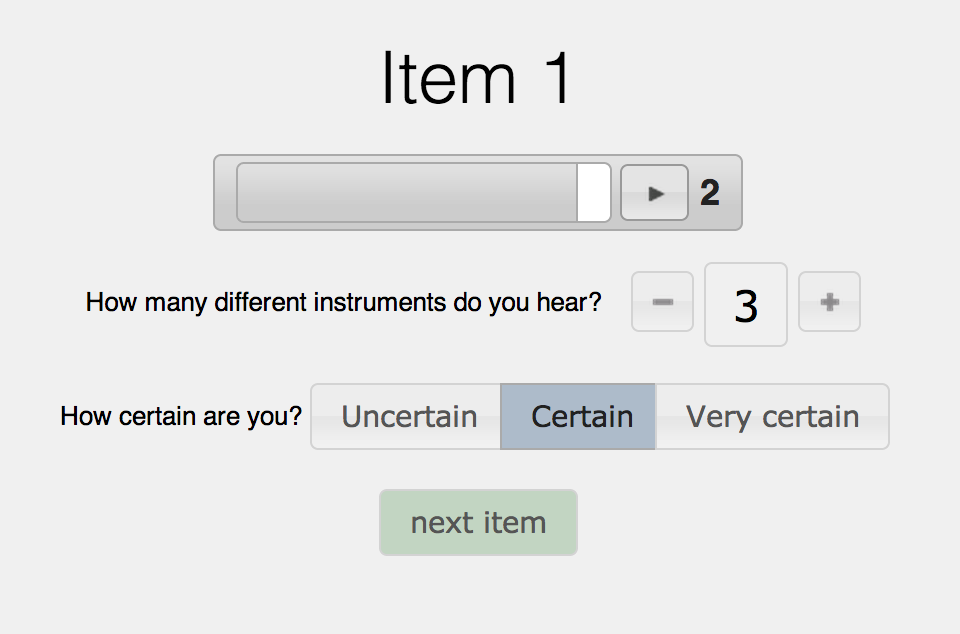
\includegraphics[width=3in]{Chapters/07_Analysis_Experiment/figures/user_interface.png}}
    \caption{Experiment User Interface}
    \label{fig:experiment_ui}
\end{figure}
Instead of a slider UI-element, the interface only features plus and minus buttons so that the subjects were not biased about the maximum number of instruments. Item \emph{J021**} had been selected as a training item and was presented to the subjects during the introduction phase to make them familiar with the user interface. This trial also unveiled the number and name of the instruments within that piece. After they had read the introduction page, the subjects were asked to adjust the volume during the training example to their preference and leave the volume at that level for the duration of the experiment. The stimuli were presented on \textsc{Beyerdynamics DT770} headphones connected to a \textsc{RME Babyface}. The complete test took about 20 minutes on average for every participant.

\subsection{Results: A gap of one instrument}

\begin{figure}[h]
\centering
\begin{minipage}{0.8\textwidth}
\begin{tabular}{c}
    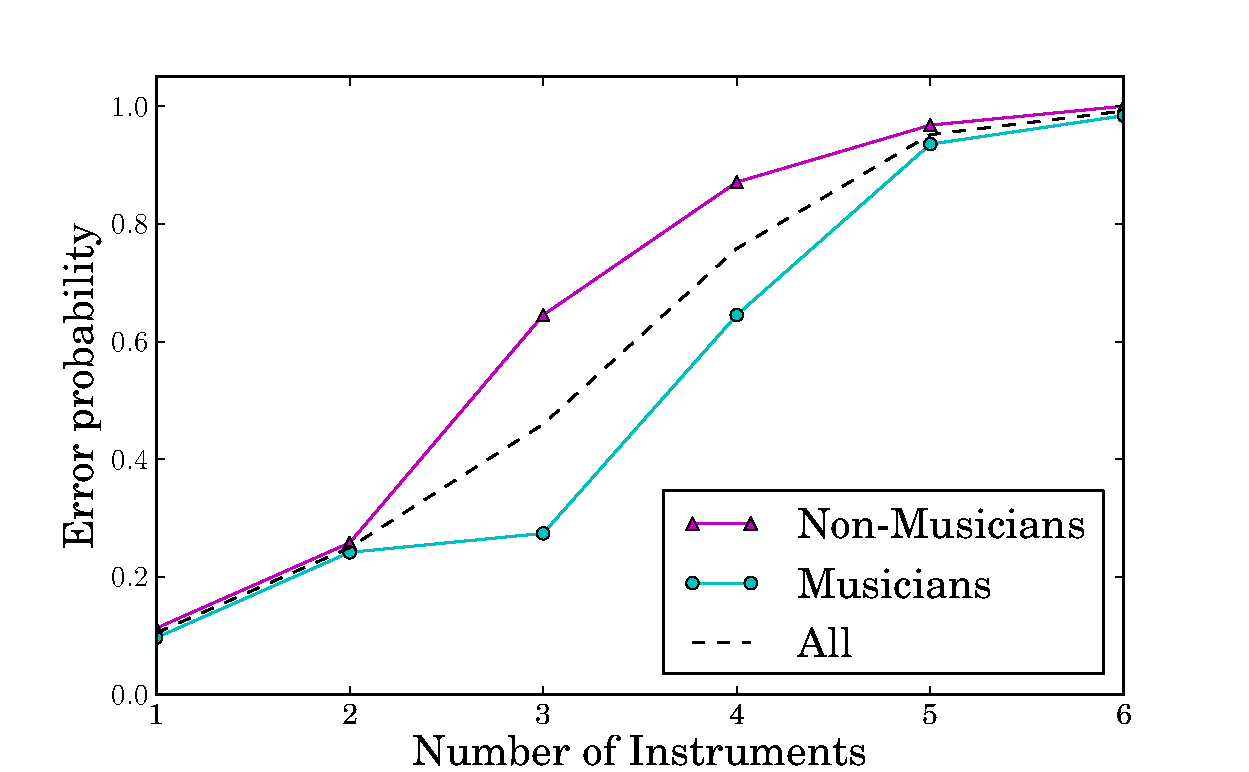
\includegraphics[width=\textwidth]{Chapters/07_Analysis_Experiment/images/error_means.pdf}
\end{tabular}
\end{minipage}
\\
\begin{minipage}{0.8\textwidth}
\begin{tabular}{c}
    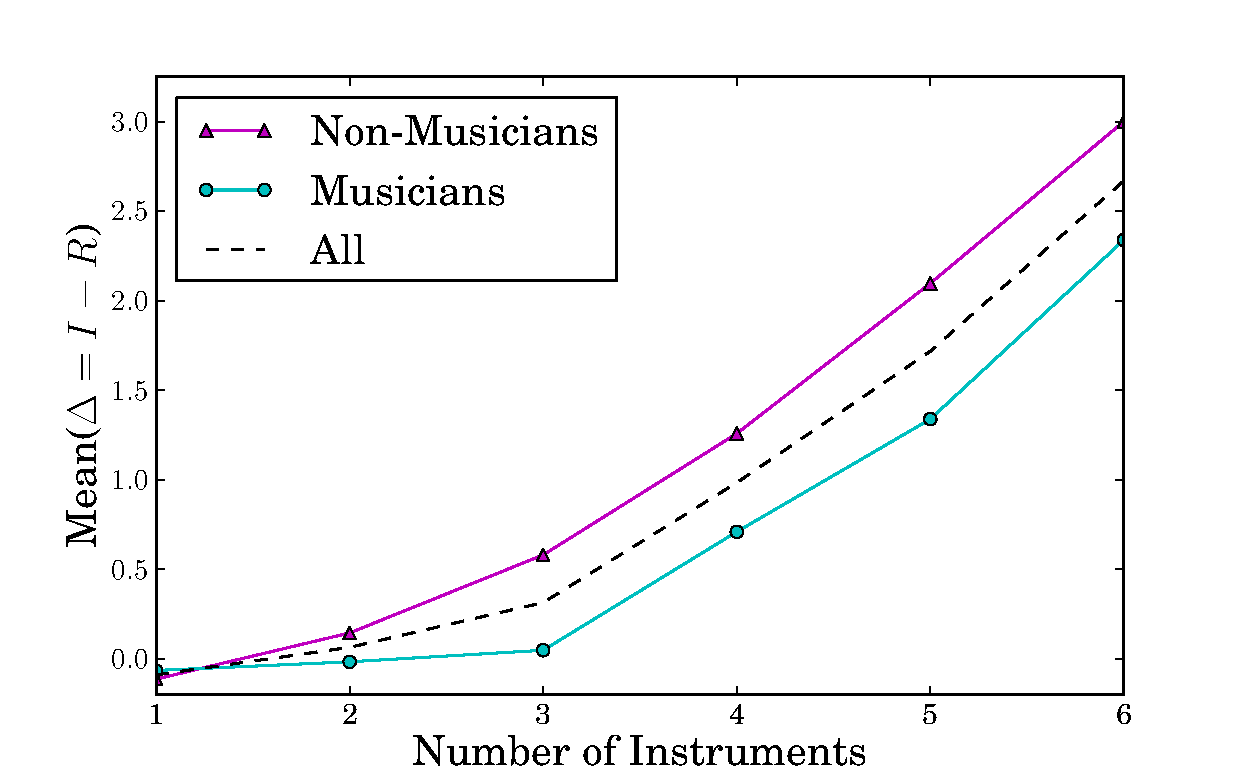
\includegraphics[width=\textwidth]{Chapters/07_Analysis_Experiment/images/error_diff.pdf}
\end{tabular}
\end{minipage}
\caption{Error probability (top) and Mean of $\Delta = I-R$ (right) categorized by the number of instruments.}
\label{fig:meanerror}
\end{figure}

The independent variable $I(i)$ is the number of instruments of one music item $i$ where in this case $I(i) \in \{1,2,...,6\}$. $R(i,s)$ is defined as the number of instruments that are perceived and counted by subject $s$ for music item $i$. The dependent variable is then derived from the main subject response as $\Delta(i,s) = I(i) - R(i,s)$ transformed into a binary scale:
\begin{align}%
\label{eq:response}
    E(i,s)&=\begin{cases}
        0 & \text{if $|\Delta| = 0 $ } \\
        1 & \text{if $|\Delta| > 0 $ .}\\
    \end{cases}
\end{align}
\par
The primary statistical null hypothesis ($H_1$) is stated in that the means of $\Delta$ and $E$\footnote{The fact that $E$ is dichotomous will lead to a mean value that equals to a probability of a binary distribution.}, grouped by the number of instruments, do not differ significantly. As we also want to test the between-groups performance of musicians versus non-musicians, we introduce another dependent variable $M(s) \in \{0,1\}$ of binary scale. This is stated in a secondary null hypothesis ($H_2$) where the means of $\Delta$ and $E$ are not significantly different between musicians and non-musicians.
No subjects were screened from the results, although there are two cases where no valid response had been made. Results are grouped by items of $I$ instruments.
\par
In general, participants tended to perform worse for items with more than two instruments. The probability of correctly estimating one instrument was 90.0\% whereas only one person out of 62 gave a correct response for an item with six instruments. In some cases, the number of instruments does not correspond to the number of voices for every item. Items where an instrument plays more than one voice and voices which are played by more than one instrument. However, most of the chosen instruments are monophonic so in our case, this occurred only for items where piano or guitar is present. Also, we made sure that the number of total voices did not exceed the maximum number of instruments in that item. Voices being played by more than one instrument (unison), present in G068, that showed surprisingly good results.

\subsubsection*{Underestimation}

We confirmed the results in~\cite{huron89} that the most common error is the underestimation of one instrument, although this accounts only for 43 \% of the responses in our experiment. Only in one case $\Delta$ is negative (overestimation) which is item C016, a ``Clarinet Quintet in A major by Wolfgang Amadeus Mozart (K.581. 1st movement)'' where we have excluded the solo clarinet part and two strings. Still, the remaining sound seems to be so similar to that of a quartet that musicians tended to hear ``phantom'' instruments.

\subsubsection*{Self-Evaluation}

Figure~\ref{fig:certainty} shows the results of the subjects certainty grouped by instrument count. Although the rate of ``very certain'' responses drops down to 11.3\% for items with six instruments the rate of ``certain'' responses is still as high as 43.5\%. When we take $\Delta$ into account we find a significant linear correlation between $\Delta$ and certainty where 0 is uncertain and 2 is very certain (Pearson's $r = -0.227$ at the $p=0.05$ level).

\begin{figure}[h]
	\centering
		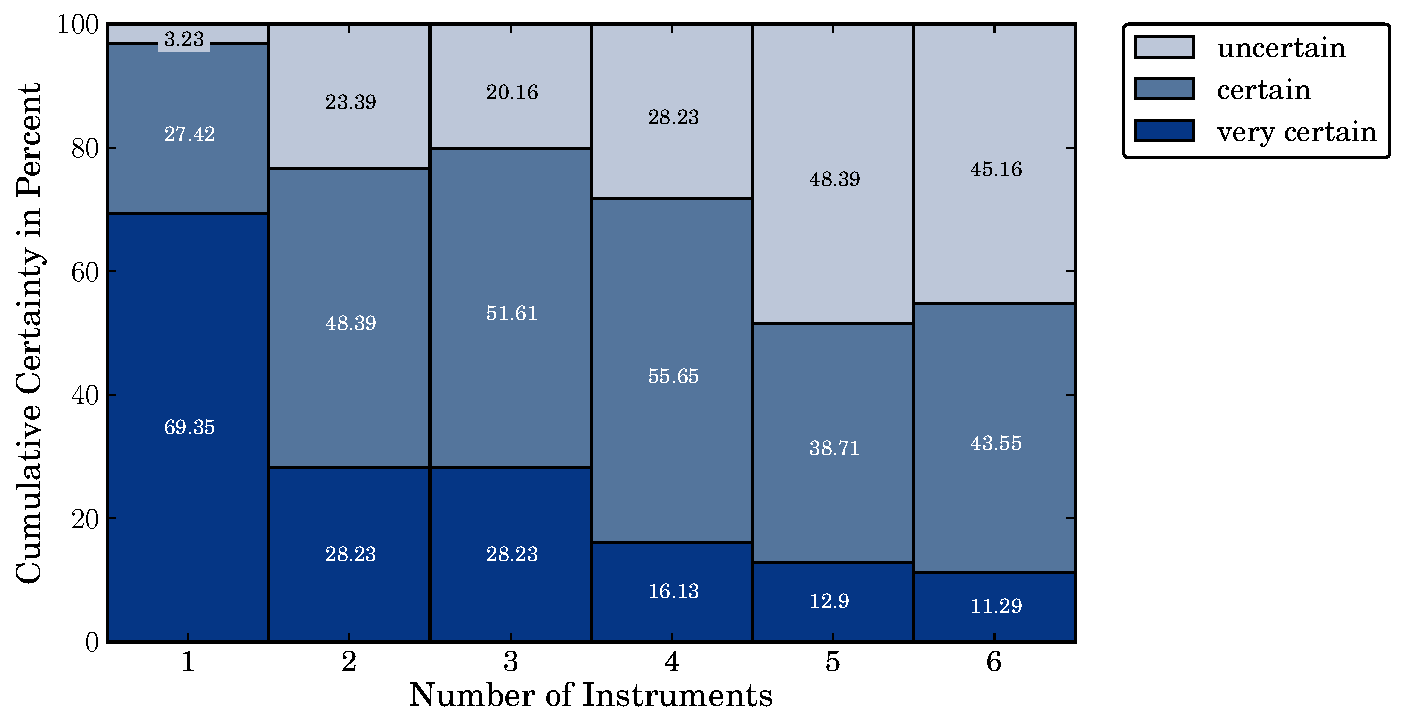
\includegraphics[height=2.5in]{Chapters/07_Analysis_Experiment/images/certainty.pdf}
	\caption{Responses for certainty of subjects by number of instruments}
	\label{fig:certainty}
\end{figure}

\subsubsection*{Main Effects}

To test the null hypotheses ($H_1$ and $H_2$), statistical tools are required.
The first tests focus on $\Delta$ which is an interval-scaled variable. To show differences between means of two or more groups, usually, One-Way-ANOVA tests are applied. ANOVA tests expect independent normally distributed variables and homogeneity of the variances in each group. However both the Kolmogorov--Smirnov test of normal distribution and Levene's test to determine the homogeneity of group variances fail. In such cases variables scaled like $\Delta$ could be transformed so that the boundaries are straightened out. A typically used $arcsin(\sqrt{\Delta})$ transformation was applied to $\Delta$ resulting in slightly higher $p$ values but still not statistically significant. Although ANOVA is known to be robust enough to run the tests against non-normal distributed cases and unequal variances, the significance levels of the results are doubtful. Therefore we choose to run a non-parametric test. The Kruskal--Wallis test can be applied even if the data is not normally distributed. However, it has to be run on a slightly modified hypothesis which compares the medians of groups instead of the means. The Kruskal--Wallis test allows to reject both modified hypotheses (asymptotic $p = 0.000$, $\chi^2 = 499636$, $df=5$).
\par
Concerning $E$ which is a categorical variable, linear models such as ANOVA cannot be used.
As described in~\cite{jaeger08}, instead, a binary regression model that turns the mean of $E$ into a binomial distributed probability can be used.
Similar to ANOVA, the output variable will be modeled by a \emph{binary logit regression} that models the output using \emph{log linear} values.
\par
By including the main factors $I$ and $M$ we set up a \emph{Generalized Linear Model} (GLM)
\begin{equation}
    logit(E) =  \text{Intercept} + x_1 \text{I} + x_2 \text{M} .
    \label{eq:logit_main}
\end{equation}
A test of the main effects is statistically significant ($\chi^2$ = $437418$, $p < 0.000$, $df = 6$) so that both null hypotheses ($H_1$ and $H_2$) can be rejected. The significance of both effects as well as parameter estimates and Wald values of the calculated model are shown in~\cite{stoeter13}.
\par
The results indicate that there is a significant difference in the error probability for groups of instrumentation counts but also for musicians versus non-musicians. A pairwise comparison test based on the mean differences reveals where these differences are located. Regarding the error probability of different instrument counts, the pairwise comparison test reveals that nearly all groups show significant mean differences between each other, which was the expected result. However, by calculation using the logit GLM model shown in equation~\ref{eq:logit_main} we found that there are two groups of items of five and six instruments (mean difference $0.04$, std. error = $0.019$, $df = 1$, $p = 0.055$) that did not show any significant difference. For both groups, the error probability is close to 100\%.
\par
To investigate the difference in performance between musicians and non-musicians a pairwise comparison between those two groups was run. Overall musicians perform about 20\% better throughout the test (mean difference = $0.18$, std. error = $ 0.0044$, $df = 1$, $p=0.000$). We do not know what caused these differences as the level of professionalism had not been surveyed. Also, 37 \% of the musicians additionally had experience in audio engineering due to their profession.
\par
Further, to look at possible interaction effects between the number of instruments and the groups of musicians and non-musicians we adapted our logit equation to
\begin{equation}
    logit(E) =  \text{Intercept} + x_1 \text{I} + x_2 \text{M} + x_3 \text{M}\times\text{I} .
    \label{eq:logit_interactions}
\end{equation}
We then reran the GLM analysis selecting only items of three and four instruments. This avoids quasi-complete separation in the logit regression model which is caused by low variances in the error probability for items of $I \in \{1,2,5,6\}$.
The model effects of the subset can be found in~\cite{stoeter13}.

\begin{figure}[h]
    \centering
    \scriptsize
    \begin{tikzpicture}[node distance=2cm]
        \draw [-,thick] (0,5*1.25) node (yaxis) [left] {$ $}
            |- (7,0.75) node (xaxis) {$ $};

        \draw (-1.1, 5) node[left,rotate=90] {Error~Probability};

        \draw (1,-0.2+0.75) -- (1,0+0.75) node[below=4pt] {musician};
        \draw (5.5,-0.2+0.75) -- (5.5,0+0.75) node[below=4pt] {non-musician};

        \draw (-0.1, 1.3710*1.25) -- (0.1, 1.3710*1.25) node[left=4pt] {$0.27$};
        \draw (-0.1, 3.2258*1.25) -- (0.1, 3.2258*1.25) node[left=4pt] {$0.65$};
        \draw (-0.1, 4.3548*1.25) -- (0.1, 4.3548*1.25) node[left=4pt] {$0.87$};

        \draw[dashed,style={color=black!35}] (0, 1.3710*1.25) -- (1.5, 1.3710*1.25) node[left=4pt] {};
        \draw[dashed,style={color=black!35}] (0, 3.2258*1.25) -- (1.5, 3.2258*1.25) node[left=4pt] {};
        \draw[dashed,style={color=black!35}] (0, 4.3548*1.25) -- (5.5, 4.3548*1.25) node[left=4pt] {};

        \GraphInit[vstyle=Normal]
        \tikzset{EdgeStyle/.style={}}
        \tikzset{colorstyle/.style={
            shape= circle,
            line width = 1pt,
            draw = black,
            fill = #1!30}
        }

        \Vertex[L=3,x=1,y=1.3710*1.25,style={colorstyle=red,line width = 4pt}] {3M}
        \Vertex[L=4,x=1,y=3.2258*1.25,style={colorstyle=blue,line width = 2pt}] {4M}
        \Vertex[L=3,x=5.5,y= 3.2258*1.25,style={line width = 4pt}] {3N}
        \Vertex[L=4,x=5.5,y=4.3548*1.25,style={colorstyle=green, draw = black!0,line width = 0}] {4N}

        \Edge[label=$0.23$,style={color=black!50}](3N)(4N)
        \Edge[label=$0.37$,style={color=black!50}](3N)(3M)

        \Edge[label=$0.23$,style={color=black!50}](4N)(4M)
        \Edge[label=$0.37$,style={color=black!50}](4M)(3M)
        \Edge[label=$0.60$,style={color=black!50}](3M)(4N)
        \Edge[label=$0.00$,style={color=red, line width = 2pt}](3N)(4M)

        \end{tikzpicture}
        \caption{Pairwise comparison between the interaction of Musician/Non-Musician and the number of instruments (labeled in nodes). The costs between nodes indicate the mean differences between groups. The red/bold line indicates that is there is no significant difference at the $p=0.005$ level.}
        \label{fig:graph}
\end{figure}
The results indicate that the interaction of Musician$\times$Instruments is not significant on a $p=0.05$ level in general and a pairwise comparison test reveals two groups of equal probability. The pairwise comparisons are depicted in Figure~\ref{fig:graph}. The red vertex indicates there is no significant difference in the error probability for the group of musicians in items with four instruments compared to non-musicians in items of three instruments. Therefore a gap in the error probability of one instrument between those two groups becomes apparent.
\par
This experiment shows that instrument count estimation tasks in music is a difficult task for humans. Our experiment with 62 participants was conducted to address the question of how many instruments one can estimate correctly.
The focus was set on stimuli of inhomogeneous timbre and also mixed genre. By comparing musicians to non-musicians, we revealed that there is a significant difference in performance. Particularly this gap is most prominent for items of three and four instruments. Furthermore, for all stimuli (ranging from one to six instruments) we see that musicians performed about 20\% better than non-musicians. The experiment shows an assumed upper limit for items with more than three instruments.

\subsection{Experiment at Larger Scale}

Many tasks in auditory experiments such as quality assessment~\cite{recommendation2001MUSHRA}, are not suitable for untrained participants, limited resources (low quality headphones, noisy environments) or time constraints.
We found that an experimental design such as count estimation, where only a single number is asked to the participant, is an ideal experimental environment to evaluate scale in an uncontrolled environment such as on the web.
We therefore designed a follow up study, published in~\cite{schoeffler13} that compares a large scale web experiment to our  laboratory results, similar to previous comparisons for other auditory tasks~\cite{Welch1996, lee2010, Salganik2006, Reips2012}.
\par
We used the same stimuli as in the laboratory experiment, however, the training phase was slightly shortened.
The experiment took place between February 2013 and April 2013 where participants visited the experimental website\footnote{{\scriptsize\url{http://www.audiolabs-erlangen.com/experiments/wice/}}}.
After a screening procedure, described in~\cite{schoeffler13}, a total of 1168 valid participants remained.
\par
The main results of the web based experiment in comparison to the previous (lab-bases) experiment is depicted in Figure~\ref{figure:error_probability_iis_vs_web}.
The figure shows the mean probability of correct responses for both environments.
The result indicate that there a only very small differences between both experiments. 
In fact, a detailed analysis in~\cite{schoeffler13} revealed that there are no statistically significant differences between the results of the two experiments. 

\begin{figure}[t]
\centering
\begin{tikzpicture}

\begin{axis}[
xlabel={Number of Instruments},
ylabel={Mean of $\textit{Resp}_{\mathrm{Correct}}$},
legend style={
font=\tiny,
ymax=1.1,
legend pos=north east,
},
legend cell align=left
]

\addplot[color=red,mark=triangle,dash pattern=on 1pt off 1pt] plot file {Chapters/07_Analysis_Experiment/plotdata/error_prob_iis_musicians.data};
\addlegendentry{Musicians [lab]}

\addplot[color=blue,mark=o,dash pattern=on 1pt off 1pt] plot file {Chapters/07_Analysis_Experiment/plotdata/error_prob_iis_non_musicians.data};
\addlegendentry{Non-Musicians [lab]}

\addplot[color=black,mark=square,dash pattern=on 1pt off 1pt] plot file {Chapters/07_Analysis_Experiment/plotdata/error_prob_iis_all.data};
\addlegendentry{All [lab]}


\addplot[color=red,mark=triangle] plot file {Chapters/07_Analysis_Experiment/plotdata/error_prob_web_musicians.data};
\addlegendentry{Musicians [web]}

\addplot[color=blue,mark=o] plot file {Chapters/07_Analysis_Experiment/plotdata/error_prob_web_non_musicians.data};
\addlegendentry{Non-Musicians [web]}

\addplot[color=black,mark=square] plot file {Chapters/07_Analysis_Experiment/plotdata/error_prob_web_all.data};
\addlegendentry{All [web]}


\end{axis}
\end{tikzpicture}
\caption{Probability of $\textit{Resp}_{\mathrm{Correct}}$ grouped by Internet experiment (web) and laboratory experiment (lab). Solid lines represent the results of the Internet experiment and dashed lines represents the results of the laboratory experiment. Figure from~\cite{schoeffler13}.}
\label{figure:error_probability_iis_vs_web}
\end{figure}

Further analysis in~\cite{schoeffler13} revealed that ``the participants in the laboratory experiment were about 4.6\% better in average for all stimuli than the participants of the Internet experiment. When looking into the differences between musicians and non-musicians, the outcome for the Internet experiment and laboratory experiment differ slightly. In the laboratory experiment musicians performed about 31.6\% better than non-musicians and in the Internet experiment musicians performed about 20.85\% better.''
Given a hypothesis that musicians are generally better at performing  certain musical related tasks, it indicates that in the (non-anonymous) laboratory experiment, participants that answered to be a musician were, on average, more professional than in the web based experiment.
\par
Finally, the experiment also showed that humans are able to correctly estimate a count even in a very challenging scenario such as unison mixtures and when asked in a not optimal environment.
In fact, the results showed that ``$76\%$ of the participants correctly identified two instruments. Only $18\%$ of the participants underestimated by one instrument, $6\%$ overestimated by one instrument.''
This surprising outcome then triggered the idea to deepen research on  unison instrumental recordings as presented in Chapter~\ref{cha:known}.

\section{Speaker Count Estimation}%
\label{sec:count_experiment}

\marginpar{This section was previously published in~\cite{stoeter19} and is reprinted, with minor modifications, with permission.}

Humans are excellent in segregating one source from a mixture~\cite{bregman90} and tend to use this skill to perceptually segregate speakers before they can estimate a count, as highlighted, e.g.\ in~\cite{kawashima15}.
As shown in~\cite{kashino96, kawashima15} with extensive experiments using Japanese speech samples, humans are able to correctly estimate up to three simultaneously active speakers without using any spatial cues.
In this experiment, we reproduced the experiments conducted in~\cite{kawashima15, kashino96} using stimuli of English speakers.
Designed to address source separation research, we also modified the question to ask participants for ``the maximum number of concurrent speakers'' in a short excerpt of speech.

\subsection{Stimuli}
To date, many available speech datasets contain recordings where only a single speaker is active.
Datasets that include overlapped speech segments either lack accurate annotations because the annotation of speech onsets and offsets in mixtures is cumbersome for humans or lack a controlled auditory environment such as in TV/broadcasting scenarios~\cite{Gravier12}.
Since a realistic dataset of fully overlapped speakers is not available, we chose to generate synthetic mixtures.
We recognize that in a simulated ``cocktail-party'' environment, mixtures lack the conversational aspect of human communication but provide a controlled environment which helps to understand how a DNN solves the count estimation problem.
As we aim for a speaker independent solution, we selected a speech corpus with preference to a high number of different speakers instead of the number of utterances, thus increasing the number of unique mixtures.
We selected \emph{LibriSpeech clean-360}~\cite{panayotov15} which includes 363 hours of clean speech of English utterances from 921 speakers (439 female and 482 male speakers) sampled at 16 kHz.
\par
To compute the maximum number of concurrent speakers \(\cardinality\), annotation of the activity of each individual speaker is required.
Even though many corpora come with word and phonemes annotation, they often are not consistent across different corpora.
We, therefore, generated annotations based on a voice activity detection algorithm (VAD). As we rely on a robust VAD estimate, we found the implementation from the \emph{Chromium Web Browser} as part of the WebRTC Standard\footnote{WebRTC 1.0: Real-time Communication Between Browsers W3C Editor's Draft 05 June 2017} to yield good results.
\par
To generate a single example, a tuple of a speech mixture and its ground truth speaker count \(\cardinality \), we draw a unique set of \(\cardinality \) speakers from the corpus.
For each of the speakers, we then select a random utterance, resampled to 16 kHz sampling rate and apply VAD.\@
The VAD method was configured using default parameters using a hop size of \SI{10}{\milli\second}.
Further, the VAD estimate was used to remove silence from the beginning and the end of an utterance recording.
In the next step, more utterances from the same speaker are drawn from the corpus until the desired duration is reached.
We removed silence in the beginning and end of each utterance to increase the overlap within one segment.
Both, the audio recording and the VAD annotation of each utterance is concatenated.
The procedure is repeated for all speakers such that \(\cardinality \) time domain signals are created.
Signals are linearly mixed and peak normalized to avoid clipping.
The ground truth output \(\cardinality \) for each sample is then computed from the VAD matrix using the maximum of the sum over all speakers.
\par
In fact, our method to generate synthetic samples results in an average overlap of 85\% for \(k=2\) and of 55\% for \(k=10\) (based on 5s segments).
This procedure is similar to~\cite{mesaros17} used to label the data.
The dataset is available for download~\cite{oss_libricount}.

\subsection{Experimental Setup}

\begin{figure}[htb]
    \centering
        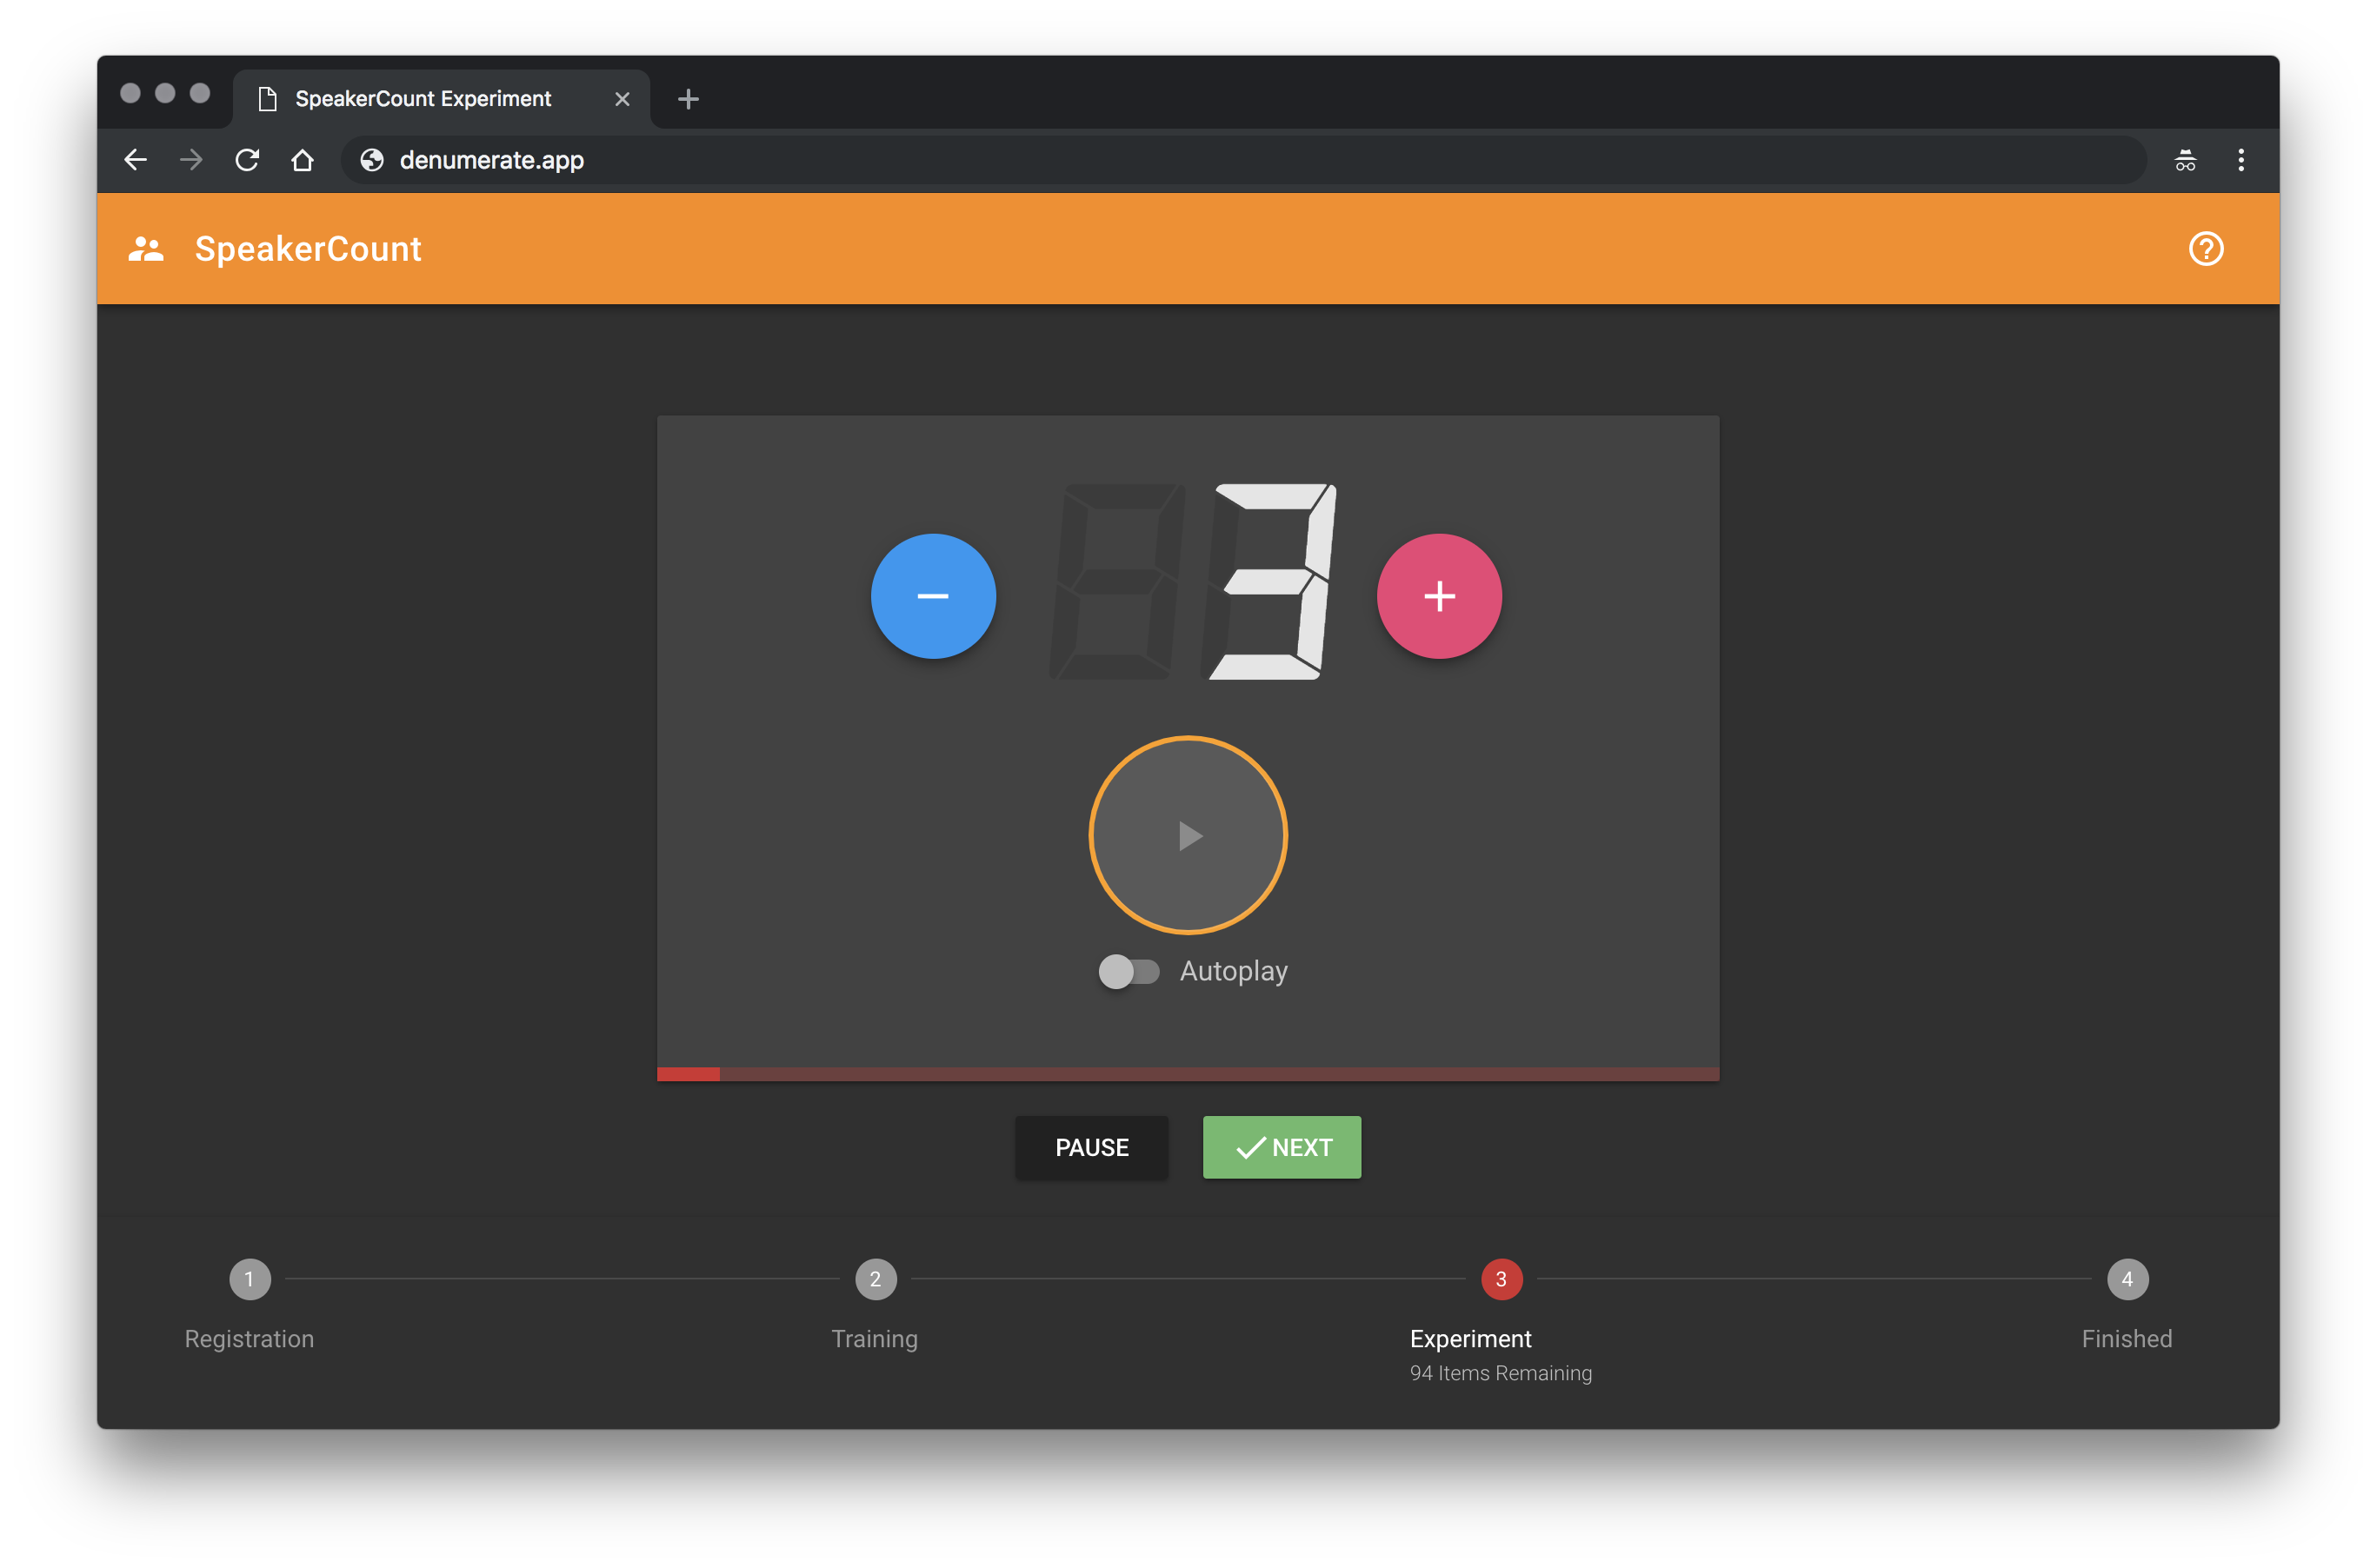
\includegraphics[width=0.9\textwidth]{Chapters/07_Analysis_Experiment/figures/experiment_ui.png}
    \caption{Speaker count estimation experiment user interface.}
    \label{fig:user_interface_speaker}
\end{figure}

We conducted a study using the simulated data from the \emph{LIBRI Count Dataset} as mentioned in the previous subsection.
In turn, we randomly selected 10 samples for each \(k \in {1, \ldots, 10}\), resulting in 100 mixtures of 5~seconds duration each.
The stimuli were presented in random order using a custom web-based interface (depicted in Figure~\ref{fig:user_interface_speaker}) connected to a database API that saved the anonymized count responses and additional information about the participant session such as the response time.
The experiment was done using \emph{between-group design}, where one group (blind experiment) did not get any prior information about the maximum number of speakers in the test set (similar to~\cite{kawashima15}).
However, the maximum number of speakers was revealed to the other group (informed experiment).
Further, none of the participants received any feedback about the error made during the trials.
The participants were able to pause and resume the experiment at any time to reduce fatigue.
Similarly to~\cite{kawashima15}, lab-based experiments were conducted with ten participants for each group (\(n=20\)) using a custom designed web-based software.
None of the participants were native English speakers.
The experiment and its results from all participants is made available through~\cite{oss_countit}.
A simplified version of the experiment is made available through a web application\footnote{\url{https://denumerate.app}}.

\subsection{Experiment Results}
To reveal over- and underestimation errors, we decided to report the average response for each group of \(k\).
As a reference, we also included the average results from~\cite[Experiment 1, 5~seconds duration]{kawashima15} which shows similar (with slightly higher error probability) results compared to our blind experiment.
Also, in~\cite{kawashima15} the maximum number of speakers to test was six whereas we evaluated stimuli with up to ten speakers.
The results of our lab-based experiments are shown in Figure~\ref{fig:experimentA} and Figure~\ref{fig:experimentB}.
Results indicate that underestimation becomes apparent for \(k > 3\).
First and foremost, we can confirm the ``one-two-three-many'' paradigm on our experiment with English utterances.
When we asked participants about the strategy they pursued, many reported that with more than three speakers it is not possible to identify (and count) the speakers but rather compare the \emph{density} of the speech to that of 1-3 speakers.
For higher speaker counts, participants reported that the phoneme density was a relevant cue that allowed them to extrapolate a source count estimate.
Interestingly, our results of the informed experiment reveal that they performed significantly better than those that participated blindly.
This is especially obvious for six and more speakers where the informed group performed better by more than one speaker in mean absolute deviation.

\begin{figure}[t!]
    \centering
    \begin{adjustbox}{width=0.7\columnwidth}
      % This file was created by matplotlib2tikz v0.6.13.
\begin{tikzpicture}

\definecolor{color1}{rgb}{0.298039215686275,0.447058823529412,0.690196078431373}
\definecolor{color0}{rgb}{0.917647058823529,0.917647058823529,0.949019607843137}
\definecolor{color4}{rgb}{0.768627450980392,0.305882352941176,0.32156862745098}
\definecolor{color2}{rgb}{0.333333333333333,0.658823529411765,0.407843137254902}
\definecolor{color5}{rgb}{0.8,0.725490196078431,0.454901960784314}
\definecolor{color3}{rgb}{0.505882352941176,0.447058823529412,0.698039215686274}

\begin{axis}[
xlabel={True \(k\)},
ylabel={Estimate \(\hat{k}\)},
xmin=-1, xmax=10,
ymin=0, ymax=11,
ytick={1,2,3,4,5,6,7,8,9,10},
xtick={0,1,2,3,4,5,6,7,8,9},
xticklabels={1,2,3,4,5,6,7,8,9,10},
tick align=outside,
tick pos=left,
ymajorgrids,
xmajorgrids,
grid style={line width=.1pt, draw=gray!20},
major grid style={line width=.2pt,draw=gray!20},
axis line style={black},
legend style={at={(0.03,0.97)}, anchor=north west, draw=none, fill=color0!20},
legend cell align={left},
legend entries={{Kawashima~\cite{kawashima15}}, {EXP (blind)}, {EXP (informed)},{Ground Truth}}
]
\addplot [only marks, mark size=2.0, mark=square*, draw=color2, fill=color2, colormap/blackwhite]
table{%
x                      y
+0.000000000000000e+00 +1.000000000000000e+00
+1.000000000000000e+00 +2.000000000000000e+00
+2.000000000000000e+00 +2.987442378071903e+00
+3.000000000000000e+00 +3.821715111593599e+00
+4.000000000000000e+00 +4.163430371330779e+00
+5.000000000000000e+00 +4.438511376242037e+00
};
\addplot [line width=1.66pt, color2, forget plot]
table {%
0 1
1 2
2 2.9874423780719
3 3.8217151115936
4 4.16343037133078
5 4.43851137624204
6 nan
7 nan
8 nan
9 nan
};
\addplot [line width=1.66pt, color2, forget plot]
table {%
0 nan
0 nan
};
\addplot [line width=1.66pt, color2, forget plot]
table {%
1 nan
1 nan
};
\addplot [line width=1.66pt, color2, forget plot]
table {%
2 nan
2 nan
};
\addplot [line width=1.66pt, color2, forget plot]
table {%
3 nan
3 nan
};
\addplot [line width=1.66pt, color2, forget plot]
table {%
4 nan
4 nan
};
\addplot [line width=1.66pt, color2, forget plot]
table {%
5 nan
5 nan
};
\addplot [line width=1.66pt, color2, forget plot]
table {%
6 nan
6 nan
};
\addplot [line width=1.66pt, color2, forget plot]
table {%
7 nan
7 nan
};
\addplot [line width=1.66pt, color2, forget plot]
table {%
8 nan
8 nan
};
\addplot [line width=1.66pt, color2, forget plot]
table {%
9 nan
9 nan
};

\addplot [only marks, mark size=2.0, mark=triangle*, draw=color3, fill=color3, colormap/blackwhite]
table{%
x                      y
+0.000000000000000e+00 +1.010000000000000e+00
+1.000000000000000e+00 +2.030000000000000e+00
+2.000000000000000e+00 +2.920000000000000e+00
+3.000000000000000e+00 +3.380000000000000e+00
+4.000000000000000e+00 +3.980000000000000e+00
+5.000000000000000e+00 +4.220000000000000e+00
+6.000000000000000e+00 +4.840000000000000e+00
+7.000000000000000e+00 +5.220000000000000e+00
+8.000000000000000e+00 +5.390000000000000e+00
+9.000000000000000e+00 +5.970000000000000e+00
};
\addplot [line width=1.66pt, color3, forget plot]
table {%
0 1.01
1 2.03
2 2.92
3 3.38
4 3.98
5 4.22
6 4.84
7 5.22
8 5.39
9 5.97
};
\addplot [line width=1.66pt, color3, forget plot]
table {%
0 1
0 1.03
};
\addplot [line width=1.66pt, color3, forget plot]
table {%
1 2
1 2.07
};
\addplot [line width=1.66pt, color3, forget plot]
table {%
2 2.78975
2 3.05
};
\addplot [line width=1.66pt, color3, forget plot]
table {%
3 3.27
3 3.5
};
\addplot [line width=1.66pt, color3, forget plot]
table {%
4 3.80975
4 4.16025
};
\addplot [line width=1.66pt, color3, forget plot]
table {%
5 4.06
5 4.4
};
\addplot [line width=1.66pt, color3, forget plot]
table {%
6 4.58
6 5.11
};
\addplot [line width=1.66pt, color3, forget plot]
table {%
7 4.97
7 5.53
};
\addplot [line width=1.66pt, color3, forget plot]
table {%
8 5.13
8 5.66
};
\addplot [line width=1.66pt, color3, forget plot]
table {%
9 5.64
9 6.29
};
\addplot [only marks, mark size=2.0, mark=diamond*, draw=color4, fill=color4, colormap/blackwhite]
table{%
x                      y
+0.000000000000000e+00 +1.000000000000000e+00
+1.000000000000000e+00 +2.030000000000000e+00
+2.000000000000000e+00 +3.100000000000000e+00
+3.000000000000000e+00 +3.830000000000000e+00
+4.000000000000000e+00 +4.590000000000000e+00
+5.000000000000000e+00 +5.400000000000000e+00
+6.000000000000000e+00 +5.950000000000000e+00
+7.000000000000000e+00 +6.200000000000000e+00
+8.000000000000000e+00 +6.630000000000000e+00
+9.000000000000000e+00 +7.460000000000000e+00
};
\addplot [line width=1.66pt, color4, forget plot]
table {%
0 1
1 2.03
2 3.1
3 3.83
4 4.59
5 5.4
6 5.95
7 6.2
8 6.63
9 7.46
};
\addplot [line width=1.66pt, color4, forget plot]
table {%
0 1
0 1
};
\addplot [line width=1.66pt, color4, forget plot]
table {%
1 1.97
1 2.1
};
\addplot [line width=1.66pt, color4, forget plot]
table {%
2 3
2 3.21
};
\addplot [line width=1.66pt, color4, forget plot]
table {%
3 3.67
3 3.98
};
\addplot [line width=1.66pt, color4, forget plot]
table {%
4 4.39
4 4.8
};
\addplot [line width=1.66pt, color4, forget plot]
table {%
5 5.16
5 5.64
};
\addplot [line width=1.66pt, color4, forget plot]
table {%
6 5.69
6 6.23
};
\addplot [line width=1.66pt, color4, forget plot]
table {%
7 5.91975
7 6.48
};
\addplot [line width=1.66pt, color4, forget plot]
table {%
8 6.34
8 6.92
};
\addplot [line width=1.66pt, color4, forget plot]
table {%
9 7.14
9 7.76025
};
\addplot [only marks, mark size=2.0, draw=color5, mark=x, fill=color5, colormap/blackwhite]
table{%
x                      y
+0.000000000000000e+00 +1.000000000000000e+00
+1.000000000000000e+00 +2.000000000000000e+00
+2.000000000000000e+00 +3.000000000000000e+00
+3.000000000000000e+00 +4.000000000000000e+00
+4.000000000000000e+00 +5.000000000000000e+00
+5.000000000000000e+00 +6.000000000000000e+00
+6.000000000000000e+00 +7.000000000000000e+00
+7.000000000000000e+00 +8.000000000000000e+00
+8.000000000000000e+00 +9.000000000000000e+00
+9.000000000000000e+00 +1.000000000000000e+01
};
\addplot [line width=1.66pt, color5, dotted, forget plot]
table {%
0 1
1 2
2 3
3 4
4 5
5 6
6 7
7 8
8 9
9 10
};
\addplot [line width=1.66pt, color5, forget plot]
table {%
0 nan
0 nan
};
\addplot [line width=1.66pt, color5, forget plot]
table {%
1 nan
1 nan
};
\addplot [line width=1.66pt, color5, forget plot]
table {%
2 nan
2 nan
};
\addplot [line width=1.66pt, color5, forget plot]
table {%
3 nan
3 nan
};
\addplot [line width=1.66pt, color5, forget plot]
table {%
4 nan
4 nan
};
\addplot [line width=1.66pt, color5, forget plot]
table {%
5 nan
5 nan
};
\addplot [line width=1.66pt, color5, forget plot]
table {%
6 nan
6 nan
};
\addplot [line width=1.66pt, color5, forget plot]
table {%
7 nan
7 nan
};
\addplot [line width=1.66pt, color5, forget plot]
table {%
8 nan
8 nan
};
\addplot [line width=1.66pt, color5, forget plot]
table {%
9 nan
9 nan
};
\end{axis}

\end{tikzpicture}

    \end{adjustbox}
    \caption{Average responses in comparison to the results of \emph{Kawashima}~\cite{kawashima15}. Error bars show 95\% confidence intervals (not available for~\cite{kawashima15}). \textsuperscript{\textregistered}2019 IEEE.}%
    \label{fig:experimentA}
 \end{figure}

\begin{figure}[t!]
   \centering
   \begin{adjustbox}{width=0.7\columnwidth}
     % This file was created by matplotlib2tikz v0.6.14.
\begin{tikzpicture}

\definecolor{color1}{rgb}{0.298039215686275,0.447058823529412,0.690196078431373}
\definecolor{color0}{rgb}{0.917647058823529,0.917647058823529,0.949019607843137}
\definecolor{color4}{rgb}{0.768627450980392,0.305882352941176,0.32156862745098}
\definecolor{color2}{rgb}{0.333333333333333,0.658823529411765,0.407843137254902}
\definecolor{color5}{rgb}{0.8,0.725490196078431,0.454901960784314}
\definecolor{color3}{rgb}{0.505882352941176,0.447058823529412,0.698039215686274}

\begin{axis}[
xlabel={true $k$},
ylabel={Proportion of Correct Responses},
xmin=-1, xmax=10,
ymin=0, ymax=1.1,
ymajorgrids,
xmajorgrids,
xtick={0,1,2,3,4,5,6,7,8,9},
xticklabels={1,2,3,4,5,6,7,8,9,10},
ytick={0,0.2,0.4,0.6,0.8,1},
yticklabels={0.0,0.2,0.4,0.6,0.8,1.0},
tick align=outside,
tick pos=left,
grid style={line width=.1pt, draw=gray!20},
major grid style={line width=.2pt,draw=gray!20},
axis line style={black},
legend entries={{EXP (blind)},{EXP (informed)},{Kawashima~\cite{kawashima15}},{Ground Truth}},
legend cell align={left},
legend style={at={(0.97,0.46)}, anchor=south east, draw=none, fill=color0!20}
]
\addplot [only marks, mark size=2.0, mark=triangle*, draw=color3, fill=color3, colormap/blackwhite]
table{%
x                      y
+0.000000000000000e+00 +9.900000000000000e-01
+1.000000000000000e+00 +9.700000000000000e-01
+2.000000000000000e+00 +6.300000000000000e-01
+3.000000000000000e+00 +3.000000000000000e-01
+4.000000000000000e+00 +1.900000000000000e-01
+5.000000000000000e+00 +6.000000000000000e-02
+6.000000000000000e+00 +4.000000000000000e-02
+7.000000000000000e+00 +4.000000000000000e-02
+8.000000000000000e+00 +1.000000000000000e-02
+9.000000000000000e+00 +2.000000000000000e-02
};
\addplot [line width=1.66pt, color3, forget plot]
table {%
0 0.99
1 0.97
2 0.63
3 0.3
4 0.19
5 0.06
6 0.04
7 0.04
8 0.01
9 0.02
};
\addplot [line width=1.66pt, color3, forget plot]
table {%
0 0.97
0 1
};
\addplot [line width=1.66pt, color3, forget plot]
table {%
1 0.93
1 1
};
\addplot [line width=1.66pt, color3, forget plot]
table {%
2 0.53
2 0.72
};
\addplot [line width=1.66pt, color3, forget plot]
table {%
3 0.21
3 0.39025
};
\addplot [line width=1.66pt, color3, forget plot]
table {%
4 0.12
4 0.27
};
\addplot [line width=1.66pt, color3, forget plot]
table {%
5 0.02
5 0.11
};
\addplot [line width=1.66pt, color3, forget plot]
table {%
6 0.01
6 0.09
};
\addplot [line width=1.66pt, color3, forget plot]
table {%
7 0.01
7 0.08
};
\addplot [line width=1.66pt, color3, forget plot]
table {%
8 0
8 0.03
};
\addplot [line width=1.66pt, color3, forget plot]
table {%
9 0
9 0.05
};
\addplot [only marks, mark size=2.0, mark=diamond*, draw=color4, fill=color4, colormap/blackwhite]
table{%
x                      y
+0.000000000000000e+00 +1.000000000000000e+00
+1.000000000000000e+00 +9.200000000000000e-01
+2.000000000000000e+00 +7.300000000000000e-01
+3.000000000000000e+00 +4.000000000000000e-01
+4.000000000000000e+00 +2.800000000000000e-01
+5.000000000000000e+00 +2.000000000000000e-01
+6.000000000000000e+00 +2.100000000000000e-01
+7.000000000000000e+00 +1.300000000000000e-01
+8.000000000000000e+00 +5.000000000000000e-02
+9.000000000000000e+00 +9.000000000000000e-02
};
\addplot [line width=1.66pt, color4, forget plot]
table {%
0 1
1 0.92
2 0.73
3 0.4
4 0.28
5 0.2
6 0.21
7 0.13
8 0.05
9 0.09
};
\addplot [line width=1.66pt, color4, forget plot]
table {%
0 1
0 1
};
\addplot [line width=1.66pt, color4, forget plot]
table {%
1 0.86
1 0.97
};
\addplot [line width=1.66pt, color4, forget plot]
table {%
2 0.64
2 0.81
};
\addplot [line width=1.66pt, color4, forget plot]
table {%
3 0.3
3 0.5
};
\addplot [line width=1.66pt, color4, forget plot]
table {%
4 0.19
4 0.37
};
\addplot [line width=1.66pt, color4, forget plot]
table {%
5 0.12
5 0.28
};
\addplot [line width=1.66pt, color4, forget plot]
table {%
6 0.14
6 0.29
};
\addplot [line width=1.66pt, color4, forget plot]
table {%
7 0.07
7 0.2
};
\addplot [line width=1.66pt, color4, forget plot]
table {%
8 0.01
8 0.1
};
\addplot [line width=1.66pt, color4, forget plot]
table {%
9 0.04
9 0.15
};

\addplot [only marks, mark size=2.0, mark=square*, draw=color2, fill=color2, colormap/blackwhite]
table{%
x                      y
+0.000000000000000e+00 +9.822222212577160e-01
+1.000000000000000e+00 +9.837037209040648e-01
+2.000000000000000e+00 +9.422222190875770e-01
+3.000000000000000e+00 +6.977777613811720e-01
+4.000000000000000e+00 +2.785184612911492e-01
+5.000000000000000e+00 +8.296289512602513e-02
};
\addplot [line width=1.66pt, color2, forget plot]
table {%
0 0.982222221257716
1 0.983703720904065
2 0.942222219087577
3 0.697777761381172
4 0.278518461291149
5 0.0829628951260251
6 nan
7 nan
8 nan
9 nan
};
\addplot [line width=1.66pt, color2, forget plot]
table {%
0 nan
0 nan
};
\addplot [line width=1.66pt, color2, forget plot]
table {%
1 nan
1 nan
};
\addplot [line width=1.66pt, color2, forget plot]
table {%
2 nan
2 nan
};
\addplot [line width=1.66pt, color2, forget plot]
table {%
3 nan
3 nan
};
\addplot [line width=1.66pt, color2, forget plot]
table {%
4 nan
4 nan
};
\addplot [line width=1.66pt, color2, forget plot]
table {%
5 nan
5 nan
};
\addplot [line width=1.66pt, color2, forget plot]
table {%
6 nan
6 nan
};
\addplot [line width=1.66pt, color2, forget plot]
table {%
7 nan
7 nan
};
\addplot [line width=1.66pt, color2, forget plot]
table {%
8 nan
8 nan
};
\addplot [line width=1.66pt, color2, forget plot]
table {%
9 nan
9 nan
};
\addplot [only marks, mark size=2.0, draw=color5, mark=x, fill=color5, colormap/blackwhite]
table{%
x                      y
+0.000000000000000e+00 +1.000000000000000e+00
+1.000000000000000e+00 +1.000000000000000e+00
+2.000000000000000e+00 +1.000000000000000e+00
+3.000000000000000e+00 +1.000000000000000e+00
+4.000000000000000e+00 +1.000000000000000e+00
+5.000000000000000e+00 +1.000000000000000e+00
+6.000000000000000e+00 +1.000000000000000e+00
+7.000000000000000e+00 +1.000000000000000e+00
+8.000000000000000e+00 +1.000000000000000e+00
+9.000000000000000e+00 +1.000000000000000e+00
};
\addplot [line width=1.66pt, color5, dotted, forget plot]
table {%
0 1
1 1
2 1
3 1
4 1
5 1
6 1
7 1
8 1
9 1
};
\addplot [line width=1.66pt, color5, dotted, forget plot]
table {%
0 nan
0 nan
};
\addplot [line width=1.66pt, color5, dotted, forget plot]
table {%
1 nan
1 nan
};
\addplot [line width=1.66pt, color5, dotted, forget plot]
table {%
2 nan
2 nan
};
\addplot [line width=1.66pt, color5, dotted, forget plot]
table {%
3 nan
3 nan
};
\addplot [line width=1.66pt, color5, dotted, forget plot]
table {%
4 nan
4 nan
};
\addplot [line width=1.66pt, color5, dotted, forget plot]
table {%
5 nan
5 nan
};
\addplot [line width=1.66pt, color5, dotted, forget plot]
table {%
6 nan
6 nan
};
\addplot [line width=1.66pt, color5, dotted, forget plot]
table {%
7 nan
7 nan
};
\addplot [line width=1.66pt, color5, dotted, forget plot]
table {%
8 nan
8 nan
};
\addplot [line width=1.66pt, color5, dotted, forget plot]
table {%
9 nan
9 nan
};
\end{axis}

\end{tikzpicture}

   \end{adjustbox}
   \caption{Mean probability of correct responses in comparison to the results of \emph{Kawashima}~\cite{kawashima15}. Error bars show 95\% confidence intervals (not available for~\cite{kawashima15}). \textsuperscript{\textregistered}2019 IEEE.}%
   \label{fig:experimentB}
\end{figure}


\section{Summary and Discussion}

In this chapter, we presented two experiments that we conducted to get a better understanding of the human ability to estimate the number of sources in overlapped mixtures.
\par
First, we showed that estimating the number of instruments in music mixtures is a challenging task for humans.
We presented the results of a controlled experiment with 62 participants, listening to stimuli of inhomogeneous timbres.
Our experiment indicated that the upper limit is reached with more than three instruments, related to an earlier experiment~\cite{huron89} focused on voices instead of instruments.
In Chapter~\ref{cha:fundamentals}, two different questions were introduced how to frame the count estimation problem.
In this experiment, we explicitly used an open question of ``How many instruments can you hear'' to gather more knowledge into the strategies being applied by the participants.
Another reason was that the stimuli durations were too long to ask for the maximum number of concurrent stimuli, thus promoting ``counting by detection'' as a good strategy to approach the problem.\par
By comparing musicians to non-musicians, we showed that there is a significant difference in performance for count estimation, confirming similar findings in other auditory tasks~\cite{kishon01}.
Particularly, we found out that this gap is most prominent for stimuli of three and four instruments.
Furthermore, for all stimuli (ranging from one to six instruments) we revealed that musicians performed about 20\% better than non-musicians, hence revealing a ``gap of one instrument'' in mean absolute error.
\par
We then repeated this experiment in an open, uncontrolled environment with more than 1000 participants.
To our knowledge, this was the first larger crowdsourced auditory experiment within the Signal Processing or MIR community.
In comparison to audio quality experiments like MUSHRA~\cite{recommendation2001MUSHRA}, we can, therefore, conclude that count estimation tasks are suitable for highly scalable crowd sourced listening experiments.
\par
In our second experiment, we reproduced an earlier study presented in~\cite{kawashima15} to estimate the maximum number of concurrent speakers in short audio mixtures, simulating a ``cocktail-party'' environment.
Our experiment went a step further with respect to the maximum amount of speakers to be estimated (up to \(k=10\)).
The results indicated almost no person was able to correctly estimate up to ten speakers.
However, we also observed that even for more than seven speakers the mean response did further (but not linearly) increase.
This indicates that humans are possibly interpolating some sort of a speech density to make up their decision.
\par
We conclude that all of our count experiments share the same results: A) humans are unable to correctly estimate more than four sources and B), underestimation is the main cause of error.
Also, we revealed that source count estimation studies can be easily be participated by non-professional listeners.
% \chapter[Data-Driven Speaker Count Estimation]{CountNet: Data-Driven Speaker Count Estimation}
\label{cha:countnet}

\marginpar{This chapter was previously published in~\cite{stoeter18, stoeter19} and is reprinted, with minor modifications, with permission (\textsuperscript{\textregistered}2019 IEEE).}

In a ``cocktail-party'' scenario, one or more microphones capture the signal from many concurrent speakers. In this setting, different applications may be envisioned such as localization, crowd monitoring, surveillance, speech recognition, speaker separation, etc.
When devising a system for such a task, it is typically assumed that the actual number of concurrent speakers is known.
This assumption turns out to be of paramount importance for the effectiveness of subsequent processing.
Notably, for separation algorithms~\cite{common10},
real-world systems do not straightforwardly provide information about the actual number of concurrent speakers.
It, therefore, is desirable to close the gap between theory and practice by devising reliable methods to estimate the number of sound sources in realistic environments.
Surprisingly, very few methods exist for this purpose in an audio context, in particular from a single microphone recording.

From a theoretical perspective, estimating the number of concurrent speakers is closely related to the more difficult problem of \textit{identifying} them, which is the topic of speaker diarization~\cite{angueramiro12, rouvier13, rouvier15, ramaiah17}.
Intuitively, if a system is able to tell who speaks when, it is naturally also able to tell how many speakers are actually active in a mixture.
We call this strategy ``counting by detection''.
A good working diarization system would be able to sufficiently address the speaker count estimation problem using this strategy.
However, it appears to be a very complex problem to tackle when one is only interested in the number of concurrent speakers.
Furthermore, as current diarization systems only work when a clear segmentation is possible, the first step of such a system often is to find homogeneous segments in the audio where only one speaker is active.
The segment borders can be found by speaker change detection~\cite{Yin17}.
These homogeneous segments are used to discriminate and temporally locate the speakers within a given recording.
When sources are simultaneously active, as in real cocktail party environments, existing segmentation strategies fail.
In fact, overlapping speech segments typically are a major source of error in speaker diarization~\cite{angueramiro12}.
\par
To improve the robustness of these detection-based methods, a number of approaches attempt to detect and possibly reject the overlapping speech segments to improve performance~\cite{boakye08, huijbregts09}.
Overlap detection has since evolved into its own line of research with many recent publications such as~\cite{geiger13, shokouhi17,andrei17}.
Overlap detection can be seen as a binarized version of the count estimation problem where the number of speakers equals to one (\emph{no overlap}) or more than one (\emph{overlap}).
It is, therefore, possible to apply a count estimation system for the overlap detection problem but not vice versa.
Also, an overlap detection system cannot be easily utilized in a source separation system.
In fact, it should be noted that before the arrival of deep learning based separation systems, models required long context and in such a case, for methods like \acs{NMF}, the number of concurrent speakers could be introduced as a regularization term~\cite{lefevre11}.
In recent years, however, large improvements were achieved by deep learning based methods~\cite{yu16, hershey16} at shorter segment duration (often 1-5 seconds).
In such approaches, it becomes possible to apply separation only when its ``needed''.
In this scenario, a method of estimating the maximum number of concurrent speakers becomes useful and in some cases essential.
\par
When speaker overlap is as prevalent as in a ``cocktail-party'' scenario, developing an algorithm to detect the number of speakers is challenging.
Since there are indications that the auditory system is capable of subitizing sources~\cite{hoopen79}, we transfer this fact to the audio domain and directly attempt in this study to estimate the number of audio sources through ``direct count estimation'' (see also Chapter~\ref{cha:countanalysis}).
The question if machines could outperform humans, or if they are subject to similar limitations, remains to be answered and is also part of this work.
\par
Directly estimating the number of sources in audio mixtures has many applications and appears as a reasonable objective that mimics the process of human perception.
Since humans do have two ears that provide spatial diversity, a first natural idea to imitate human performance is to exploit \textit{binaural} information to proceed to source count estimation.
In terms of signal processing, this is achieved by estimating directions of arrival (DoA) and clustering them~\cite{loesch08, araki09, arberet10, pavlidi12, drude14_icassp, mirzaei15, walter15, Pasha17_reverb}.
However, many audio devices are equipped with only a single microphone, and being able to also count sources, in that case, is desirable.
Consequently, the single-channel scenario has been considered in many studies.
\par
One of the first single-channel methods was proposed in 2003 by Arai~\cite{arai03}.
It is based on the assumption that speech mixed from more than one speaker has a more complex amplitude modulation pattern than a single speaker.
The modulation pattern is aggregated and used as a decision function to distinguish between different numbers of speakers.
In~\cite{sayoud10}, the authors propose an energy feature based on temporally averaged mel filter outputs.
The number of concurrent speakers was determined by manually determining thresholds that best match individual speaker counts.
In a more recent work,
Xu et.al.~\cite{xu13} estimate the number of speakers by applying hierarchical clustering to fixed-length audio segments using mel frequency cepstral coefficients (MFCCs) and additional pitch features.
The method assumes the presence of at least some non-overlapped speech and was evaluated on real-world data of 20 hours duration.
An average count estimation error of one speaker is reported using excerpts of eight-minutes duration and featuring up to eight speakers.
In another vein, Andrei et.al.~\cite{andrei15, andrei15a} proposed an algorithm which correlates single frames of multi-speaker mixtures with a set of single-speaker utterances.
The resulting score was then used to estimate the number of speakers using thresholds.
\par
In all the aforementioned methods, the speaker count estimation problem was devised.
The different strategies undertaken there rely on classical and grounded signal processing strategies and exhibit fair performance in a controlled setup.
However, our experience shows (see Section~\ref{sec:evaluation}) that they leave much room for improvement when applied to more diverse and challenging signals than those corresponding to their targeted applications, notably in the case of many different and constantly overlapping speakers.
This is due to their main common weakness, which is to rely on the assumption that there are segments where only one speaker is active, in a way that is similar to the classical speaker diarization studies mentioned before.
In~\cite{stoeter17} we presented a first data-driven approach based on a recurrent network, motivated by the recent and impressive successes of deep learning approaches in audio tasks such as speech separation~\cite{yu16, hershey16, grais17} and speaker diarization~\cite{yella14, hruz16, garciaromero17}.
The methods proposed in~\cite{stoeter17} to address speaker count estimation were built upon recent methods to count objects in images, which is a popular application with many contributions from the deep learning community~\cite{wang15, chattopadhyay17, khan16, segui15, zhang15, arteta16, marsden16, boominathan16, zhang2015salient}.
In~\cite{stoeter17} two main paradigms were evaluated: a) count estimation as regression problem, where the systems are directly trained to output the number of objects as a point estimate, and b) classification, where every possible number of objects is encoded as a different class and the output of a predicting system corresponds to a probability distribution over these classes.
The results of the proposed method indicated that a classification based neural network performed better than one based on regression.
One drawback, however, is that the maximum number of speakers (the number of classes) is known in advance.
\par
In this study, we build upon~\cite{stoeter17} and focus on the network architecture design, as well as on finding limitations for different test scenarios.
This work makes the following contributions:
i) we generalize the problem formulation by fusing classification and regression, which allows estimating discrete outputs while controlling the error term. This is done by picking a point estimate from a full posterior distribution provided by the deep architectures;
ii) in addition to the recurrent network introduced in~\cite{stoeter17}, we propose alternative speaker-independent neural network architectures based on the convolution operation to improve count estimation.
Each of the proposed networks is adjusted to estimate the number of speakers from audio segments of 5 seconds;
iii) we test the performance of these networks in multiple experiments and compare them to several baseline methods, pointing out possible limitations.
Furthermore, we present a statistical analysis of the results to determine whether classification outperforms regression for all architectures;
iv) we conducted a listening experiment to relate the best-performing machine to human performance.
We describe one of the strategies taken by the data-driven approach that might explain its superior performance.
Finally, for the sake of reproducibility, the trained networks (models), as well as the test dataset, are made available on the accompanying website\footnote{\url{https://www.audiolabs-erlangen.de/resources/2017-CountNet}.}.

\section{Problem Formulation}%
\label{sec:problem_formulation}
We consider the task of estimating the maximum number of concurrent speakers \( \cardinality \in \mathbb{Z}^{+}_{0} \) in a single-channel audio mixture \(\mathbf{x}\).
This is achieved by applying a mapping from \(\mathbf{x}\) to \(\cardinality \).
We now provide details on the notations, the general structure of the method, and ways to exploit the deep learning framework to estimate \(\cardinality \).

\subsection{Signal Model}%
\label{ssec:signal_model}
Let \(\mathbf{x}\) be a time domain vector with \(N\) samples, representing a linear mixture of \(L\) single speaker speech signal vectors \(\mathbf{s}_l\).
The value observed at time instant~\(n\) for the mixture is given by~$x_n$ and for the individual speech segments by~$s_{nl}$.
The mixture then results in
%
\begin{equation}
  x_n = \sum_{l=1}^{L}{s_{nl}} \;  n \in \{ 1,\ldots, N \}.
  \label{eq:mixing_model}
\end{equation}
%
Naturally, each speaker~$l=1,\dots,L$ is not active at every time instant.
On the contrary, we assume there is a latent binary \textit{speech activity} variable~$v_{nl}\in \left\{ 0,1 \right\}$ that is either provided by a ground truth annotation or computed using a voice activity detection method.

Our objective of estimating the maximum number of concurrent speakers can now be formulated as

\begin{equation}
k=\underset{n}{\max}\left(\sum_{l = 1}^{L} v_{nl}\right) \; n \in \{ 1,\ldots, N \}
\label{eq:definition_k}.
\end{equation}

As can be seen, our proposed task of estimating $k\leq L$, is more closely related to source separation whereas the estimation of \(L\) is more useful for tasks where speakers do not overlap (see Section~\ref{sub:count_problemstatement}).
For instance, three non-overlapping speakers would result in \(L = 3\) and \(\cardinality = 1\).
It should be noted that at short time scales both task definitions provide the same outcome because on such a time scale the speaker configuration usually does not change. The problem arises for long-term recordings (e.g. larger than ten seconds) which are not considered in this work.
In any case, we want to emphasize that in all experiments presented in this Chapter, we made sure that for all audio segments $k = L$.
\par
In the remainder of this chapter, we assume that no additional prior information about the speakers is given to the system except possibly the maximum number of concurrent speakers~$k_{\max}$, that is application-dependent and represents an upper bound for the estimation.

While speaker diarization would mean estimating the whole speech activity matrix~$v_{nl}$, our problem of estimating only~$k$ in~(\ref{eq:definition_k}) is more abstract as it requires a direct estimation of the count.

By processing such excerpts in a sliding-window fashion, our proposed solution can be applied straightforwardly to context sizes commonly used in source separation.
Furthermore, our proposed system can be used also to detect overlap ($k > 1$), which can be useful as a pre-processing step for diarization.

Now, the system we propose is actually not inputting the signal vector $\mathbf{x}$, but rather a Time-Frequency (TF) representation as the absolute value of the short-time Fourier transform of~$\mathbf{x}$ that is denoted by $\mathbf{X}$.
In the following, $\mathbf{X}$ is the non-negative input for the system.

\subsection{Probabilistic Formulation}%
\label{ssec:model}
In a supervised scenario, let~$ \left\{\mathbf{X}_t,k_t\right\}_t$ be all of our learning examples, where~$t \in{1,\dots,T}$ denotes the $t$-th training item from the training database.
For the purpose of learning a mapping between~$\mathbf{X}$ and~$k$, we adopt a probabilistic viewpoint and introduce a flexible generative model that explains how a particular source count~$k$ corresponds to some given input ~$\mathbf{X}$.

First, we consider that all training samples~$\left\{\mathbf{X}_t,k_t\right\}_t$ are independent.
For each sample, we consider that~$k_t$ is drawn from a probability distribution of a known parametric family, parameterized by some latent and unobserved parameters~$\mathbf{y}_t$
\begin{equation}
\mathbb{P}\left(k_{t}\mid\mathbf{X}_{t}\right)=\mathcal{L}\left(k_{t}\mid \mathbf{y}_{t}\right),
\end{equation}
the distribution~$\mathcal{L}\left(\cdot\mid \mathbf{y}_{t}\right)$ is called the \textit{output distribution} in the following.
We further assume that there is some deterministic mapping between~$\mathbf{X}_t$ and~$\mathbf{y}_t$, embodied as
\begin{equation}
\mathbf{y}_{t}=f_{\boldsymbol{\theta}}\left(\mathbf{X}_{t}\right),
\end{equation}
where $\boldsymbol{\theta}$ are the parameters for this deterministic mapping, that is independent of the training item~$t$. This results in an output distribution given by
\begin{equation}
\mathbb{P}\left(k_{t}\mid\mathbf{X}_{t}\right)=\mathcal{L}\left(k_{t}\mid f_{\boldsymbol{\theta}}\left(\mathbf{X}_{t}\right)\right).\label{eq:output_distribution}
\end{equation}
Assume for the rest of this section that these parameters~$\boldsymbol{\theta}$ are known.
Given a previously unseen input~$\mathbf{X}$, expression~(\ref{eq:output_distribution}) means we can compute the distribution of the source count~$k$.
The objective of our count estimation system is to produce a point estimate~$\hat{k}$ rather than a whole output distribution~$\mathbb{P}\left(k\mid\mathbf{X}\right)$.
A first option is to pick as an estimate the most likely outcome for the output distribution, thus resorting to Maximum A Posteriori (MAP) estimation:
\begin{equation}
\hat{k}=\underset{k}{\text{argmax}}\ \mathcal{L}\left(k\mid f_{\boldsymbol{\theta}}\left(\mathbf{X}\right)\right).
\end{equation}
However, MAP is not the only option and a broad range of point estimation techniques may be obtained when resorting to decision theory~\cite{berger1985}.
We may for example also choose~$\hat{k}$ as the value that minimizes the marginal average cost of choosing an estimate $\hat{k}$ instead of the true value $k$, when $k$ is distributed with respect to the output distribution
\begin{equation}
\hat{k}=\underset{u}{\text{argmin}}\intop_{k}d\left(k,u\right)\mathcal{L}\left(k\mid f_{\boldsymbol{\theta}}\left(\boldsymbol{X}\right)\right) \mathrm{d} k,\label{eq:estimate_hatk}
\end{equation}
where $d\left(k,u\right)$ is the cost of picking $u$ as an estimate when the true value is~$k$.
It may be any function that seems appropriate, and does not necessarily need to be differentiable.
However, we retain the more general formulation~(\ref{eq:estimate_hatk}) because other choices will sometimes prove more effective, as we show later.
For notational convenience, we write~(\ref{eq:estimate_hatk}) as
\begin{equation}
\hat{k}=q\left(f_{\boldsymbol{\theta}}\left(\boldsymbol{X}\right)\right),
\end{equation}
and $q\left(\cdot\right)$ is called the~\textit{decision function}.
Using this strategy, we have everything to produce a single source count estimate~$\hat{k}$ from input features~$\mathbf{X}$, provided the parametric family~$\mathcal{L}$ and the mapping $f_{\boldsymbol{\theta}}$ as well as its parameters $\boldsymbol{\theta}$ are known.
In this study, we choose a deep neural network for the mapping $f_{\boldsymbol{\theta}}$, whose weights~$\boldsymbol{\theta}$ are trained in a supervised manner (compare Figure~\ref{fig:blockdiagram}).
Once a particular network architecture has been chosen, learning its parameters is achieved through classical stochastic gradient descent.
If we assume that the particular family~$\mathcal{L}$ of output distributions has been chosen, it appears natural to learn the parameters~$\boldsymbol{\theta}$ that maximize the likelihood of the learning data.
More specifically, the total cost to be minimized becomes
\begin{equation}
C=\sum_{t=1}^{T}-\log\mathcal{L}\left(k_{t}\mid f_{\theta}\left(\boldsymbol{X}_{t}\right)\right).\label{eq:total_cost}
\end{equation}
The derivative of this cost (\ref{eq:total_cost}) with respect to the parameters can be used to learn the network parameters.
\par
Three different choices for the family of output distributions (classification, Gaussian regression and Poisson regression) are summarized below.

\begin{figure}[t]
  \centering
  \begin{adjustbox}{width=.8\textwidth}
    \begin{tikzpicture}[>=stealth, auto, node distance=4cm]
    \tikzstyle{every path}=[line width=0.4mm]
    % Place nodes
    % Define the style for the blue dotted boxes
    \tikzset{blue dotted/.style={draw=blue!80!white, line width=1pt,
                          dash pattern=on 1pt off 1pt on 1pt off 1pt,
                           inner sep=4mm, rectangle, rounded corners}};
    \tikzset{red dotted/.style={draw=red!80!white, line width=1pt,
                           dash pattern=on 1pt off 1pt on 1pt off 1pt,
                           rectangle}};
    \tikzstyle{red text}=[text=red!80]
    \tikzstyle{blue text}=[text=blue!80]
    \tikzstyle{block} = [draw, rectangle, inner sep=3pt, minimum width=3cm, minimum height=1cm, align=center]
    \tikzstyle{pinstyle} = [pin edge={to-,thin,blue!80}]
    \tikzstyle{pinstyle2} = [pin edge={-to,thin,red!80, dash pattern=on 1pt off 1pt on 1pt off 1pt}]


    \node [block] (feat) {Feature Extraction};
    \node [block, right of=feat, node distance=4cm] (norm) {Normalisation +\\Standardization};
    \node [block, right of=norm, pin={
      [pinstyle, blue text, name=k_train]above:$k$
    }] (dnn) {DNN};
    \node [block, red dotted, red text, below of=dnn, pin={[pinstyle2, red text, name=k_inf]right:$\hat{k}$}, node distance=2cm] (inference) {q};
    \coordinate [left of=feat, node distance=2cm] (input) {};
    \node at ($(k_train.east)+(11mm, 0)$) [blue text, above, inner sep=3mm] {\textbf{Training}};
    \node at ($(inference.south east)+(0, -3mm)$) [red text, below, inner sep=3mm] {\textbf{Inference}};

    % Connect nodes
    \draw [->] (input) -- node {$x$} (feat);
    \draw [->] (feat) -- node {$\mathbf{X}$} (norm);
    \draw [->] (norm) -- (dnn);
    \draw [dash pattern=on 1pt off 1pt on 1pt off 1pt, ->] (dnn) -- node {$y$} (inference);

\end{tikzpicture}

  \end{adjustbox}
\caption{%
Block diagram of the proposes supervised learning model.
Training is realised using tuples of spectro-temporal inputs \(\mathbf{X}\) and
the true number of concurrent speakers \(k\). For inference the output \(y\) is post-processed using a decision function \(q\) to generate estimates \(\hat{k}\). \textsuperscript{\textregistered}2019 IEEE.
}%
\label{fig:blockdiagram}
\end{figure}

\subsubsection{Classification}
In a classification setting, the output distribution is directly taken as \textit{discrete}, discarding any meaning concerning the ordering of the different possible values.
Given some particular input~$\mathbf{X}$, the network generates the posterior output probability for \((k_{\max} + 1)\) classes (including \(k=0\)) and a maximum a posteriori (MAP) decision function is chosen that simply picks the most likely class \(q = \arg\max(\cdot)\).
Classification based approaches have successfully been applied in deep neural networks for estimating counts in objects~\cite{segui15, zhang2015salient, khan16} in images.

\subsubsection{Gaussian Regression}
In regression, $k$ is derived from an output distribution defined on the real line.
However, this comes with the additional difficulty of handling the fact that~$k$ is integer.

The output distribution in this setting is assumed to be Gaussian and the associated cost function is the classical squared error.
During inference and given the output~$f_{\boldsymbol{\theta}}\left(\mathbf{X}\right)$ of the network, the best discrete value that is consistent with the model is simply the rounding operator $q = \left[\cdot\right]$.

Gaussian regression has achieved state-of-the-art count estimation performance in computer vision using deep learning frameworks~\cite{zhang15, marsden16, boominathan16}.

\subsubsection{Discrete Poisson modeling}
When it comes to modeling count data, it is often shown effective to adopt the Poisson distribution~\cite{fallah09}.
First, this strategy retains the advantage of the classification approach to directly pick a probabilistic model over the actual discrete observations, avoiding the somewhat artificial trick of introducing a latent variable that would be rounded to yield the observation.
Second, the model avoids the inconvenience of the classification approach to completely drop dependencies between classes.

Due to these advantages, the Poisson distribution has been used in studies devising deep architectures for count estimation systems~\cite{Rezatofigh16}.
For instance in~\cite{fallah09, chan09, Rezatofigh16}, it is shown that the number of objects in images can be well modeled by the Poisson distribution. Inspired by these previous works, we also consider the Poisson output distribution \(\mathcal{P}\left(k\mid f_{\boldsymbol{\theta}}\left(\mathbf{X}\right)\right)\) where $\mathcal{P}\left(\cdot\mid\lambda\right)$ denotes the Poisson distribution with scale parameter~$\lambda$.

In that setup, the cost function at learning time is the Poisson negative log-likelihood and the deep architecture at test time provides the predicted scale parameter $f_{\boldsymbol{\theta}}\left(\mathbf{X}\right)\in\mathbb{R}_+$, which summarizes the whole output distribution.

As a decision function~$q$ in this setting, we considered several alternatives. A first option is to again resort to MAP estimation and pick the mode $\left[f_{\boldsymbol{\theta}}\left(\mathbf{X}\right)\right]$ of the distribution as a point estimate. However, experiments showed that the posterior median yields better estimates, and is given by
\begin{subequations}
\begin{align}
q\left(f_{\boldsymbol{\theta}}\left(\mathbf{X}\right)\right) & =\underset{\hat{k}}{\text{argmin}}\sum_{k=0}^{\infty}\left|\hat{k}-k\right|\mathcal{P}\left(k\mid f_{\boldsymbol{\theta}}\left(\mathbf{X}\right)\right)\\
 & =\text{median}\left(k\sim\mathcal{P}\left(f_{\boldsymbol{\theta}}\left(\mathbf{X}\right)\right)\right)\\
 & \approx\left\lfloor f_{\boldsymbol{\theta}}\left(\mathbf{X}\right)+\frac{1}{3}-\frac{0.02}{f_{\boldsymbol{\theta}}\left(\mathbf{X}\right)}\right\rfloor, \label{eq:decision_function_poisson}
\end{align}
\end{subequations}
where the last expression is an approximation of the median of a Poisson distributed random variable of scale parameter~$f_{\boldsymbol{\theta}}\left(\mathbf{X}\right)$~\cite{Choi94}.

\section{DNNs for Count Estimation}%
\label{sec:supervised_learning}

Applying deep learning to an existing task often is a matter of choosing a suitable network architecture.
Typically an architecture describes the overall structure of the network including (but not limited to) the type and number of layers in the network and how these layers are connected to each other.
In turn, designing such an architecture requires deep knowledge about input and output representations and their required level of abstraction.
Many audio-related applications like speech recognition~\cite{HintonSpeech} or speaker diarization share similar common architectural structures, often found by incorporating domain knowledge and through extensive hyper-parameter searches.
For our task of source count estimation, however, domain knowledge is difficult to incorporate, as our studies aim at revealing the best strategy to address the problem.
This is why we chose architectures that already have shown a good level of generalizability for audio applications.

\subsection{Network Architectures}
The input of all networks is a batch of samples, represented as time-frequency representations \(\mathbf{X} \in \mathbb{R}^{ D \times F \times C } \), where \(D\) refers to the time dimension, \(F\) to the frequency dimension and \(C\) to the channel dimension (in the single-channel case, \(C=1\)).
In the following, we discuss several commonly used DNN architectures and their benefits in using them for the task of estimating the number of speakers.
All architectures under investigation are summarized in Fig.~\ref{fig:networkoverview}.

\subsubsection{Convolutional Neural Networks (\acs{CNN})}%
Convolutional Neural Networks (CNNs) are a variant of standard fully-connected neural networks, where the architecture generally consists of one or more ``convolution layers'' followed by fully-connected layers leading to the output.

A convolutional layer consists of a convolution operation, followed by feature pooling.
The convolution operation applies a set of filters to local regions of the input, and the application of each such filter outputs a \emph{feature map}.
It should be noted that the convolution operation, generally, also constitutes the application of a point-wise non-linear activation function on each feature map.
This is followed by feature pooling, that aims to reduce the feature space dimensions by combining the filter activations over a specified region.
Since the individual elements of the filters (weights) are learned during the training stage, convolutional layers can also be interpreted as feature extractors.
By stacking up additional layers, CNNs can extract more abstract features in higher level layers~\cite{Simonyan15}.
\par
The sizes of the filter kernels are crucial, and it was shown in~\cite{pons2017timbre} that many audio applications can benefit if domain knowledge is put into the design of the filter kernel size.
The use of small filter kernels, as often used in image classification tasks, does not necessarily decrease performance, when combined with many layers.
Also larger kernels increase the number of parameters and therefore the computational complexity.
It was shown in~\cite{schluter15} that \(3 \times 3\) kernels resulted in state-of-the-art results in singing voice detection tasks.
Due to its hierarchical architecture, CNNs with small filters have the benefit that they can model time and frequency invariances regardless of the scaling of the frequency axis.
\par
Our proposed architecture is similar to the ones proposed by ~\cite{schluter16} used for singing voice activity detection.
In our proposed CNN, we consider local filters of size \(3 \times 3\). In the first layer, 2D convolution is performed by moving the filter across both dimensions of the input in steps of 1 element (striding \(s = 1\) to generate \(C = 64\) feature maps/channels resulting in an output volume of \(64 \times (D - 3 + 1) \times (F - 3 + 1)\).
In the subsequent convolution layers, a similar operation is applied but for each convolutional layer, we consider a different number of feature maps.
Note, that the convolution operation is performed independently for every input channel, and then summed up along the dimension \(C\) for each output element.
In preliminary experiments we found that by using max-pooling we received significantly better performance when used after CNN layers.

\subsubsection{Recurrent Neural Networks (RNN)}%
A recurrent neural network (RNN) layer is very similar to a fully connected network, except that RNN applies the same set of weights \(\mathbf{A}\) recursively over an input sequence.
While convolutional layers excel in capturing local structures, RNNs can detect structure in sequential data of arbitrary length. %have an internal memory of infinite length of the past input sequence history.
This makes it ideal to model time series, however, in practice, the temporal context learnt is limited to only a few time instances, because of the vanishing gradient problem~\cite{Hochreiter98}.

To alleviate this problem, forgetting factors (also called gating) were proposed.
One of the most popular gated recurrent cells is the Long Short-Term Memory (LSTM)~\cite{Hochreiter97} cell.
Its effectiveness has been proven in applications and LSTMs are the state-of-the-art approach for speech recognition~\cite{Graves13} and singing voice detection~\cite{Leglaive15}~\footnote{For a deeper mathematical background of LSTMs, due to space constraints, the reader is referred to the aforementioned papers.}.
For a given input of dimensions \(D \times F \times C\), the output of a recurrent layer is either only the last step of dimension \(1 \times A\) or the full sequence \(D \times A\).
The latter is useful to stack multiple LSTMs or to apply temporal max pooling of the sequence.
In~\cite{stoeter17} such an architecture based on three bi-directional LSTM cells, was proposed. The architecture is similar to the one employed in~\cite{Leglaive15}.

\subsubsection{Convolutional Recurrent Neural Networks (CRNN)}%
Recently, a combination of convolutional and recurrent layers were proposed for audio-related tasks~\cite{sainath15, amodei16, Choi17, cakir17}.

The main motivation to stack these layers is to combine the benefits of convolutional layers with those of recurrent architectures, namely the benefit of convolutional layers in aggregating local features with the ability of recurrent layers to model long-term temporal data.

There are different ways to stack CNNs and RNNs to form a CRNN architecture.
In our application the motivation is to aggregate local time-frequency features coming from the output convolutional neural network and use the LSTM layer to model long temporal structures.
As the output of a CNN layer is a 3D volume \(D \times F \times C\) and the input of a recurrent layer only takes a 2D sequence, the dimension would need to be reduced. Naturally, the time dimension would need to be kept, therefore the channel dimension \(C\) is stacked with the frequency dimension \(F\) resulting in a \(D \times F \cdot C\) output.

\subsubsection{Full-band Convolutional Neural Networks (F-CNN)}%

Architectures where filters span the full frequency range and therefore apply convolution in temporal direction only, have already been successfully deployed in speech~\cite{amodei16} and music application~\cite{Choi17, pons16, Dieleman14}).
Our motivation here is that the activity of speakers happen over wide frequency ranges and a count (unlike in counting objects in images) cannot be split into sub counts.
The full-band kernel configuration only affects the first hidden layer, as in consecutive outputs all frequency bands are squashed down to one single frequency band using ``valid'' convolutions.
This is computationally very efficient, because it reduces the middle layer's dimensionality of the network significantly due to this aggregation.
To further optimize the performance of the network, we applied a hyper-parameter optimization technique using Tree-structured Parzen Estimator (TPE)~\cite{bergstra11}.
We used a search space of several hyper-parameters as shown in Table~\ref{tab:fcnnhyper} and set the maximum number of evaluations to 200.

\begin{table}
  \centering
  \scriptsize
\begin{tabular}{lll}
  \toprule
  Layer               & Parameters        & Value Range \\
  CNN 1               & Feature Maps      & \( \{16, \mathbf{32}, 64\} \) \\
  CNN 1               & Filter Length     & \( \{\mathbf{3}, 5, 7\} \) \\
  Pooling 1           & Pooling Length    & \( \{1, \mathbf{2}, 4\} \) \\
  CNN2                & Feature Maps      & \( \{16, \mathbf{32}, 64\} \) \\
  CNN2                & Filter Length     & \( \{\mathbf{3}, 5, 7\} \) \\
  Pooling 2           & Pooling Length    & \( \{1, 2, 4\} \) \\
  \midrule
  CNN 3               & Presence of Layer & \( \{\mathbf{Yes}, No\} \) \\
  CNN 3               & Feature Maps      & \( \{16, 32, \mathbf{64}, 128\} \) \\
  CNN 3               & Filter Length     & \( \{\mathbf{3}, 5, 7\} \) \\
  Pooling 3           & Pooling Length    & \( \{1, \mathbf{2}, 4\} \) \\
  \midrule
  Fully Connected 1   & Hidden Unit       & \( \{64, \mathbf{128}\} \) \\
  Dropout 1           & Dropout Percentage& \( [0.1, \mathbf{0.2}, 0.5] \) \\
  Fully Connected 2   & Hidden Unit       & \( \{32, \mathbf{48}\} \) \\
  Dropout 2           & Dropout Percentage& \( [0.1, \mathbf{0.2}, 0.5] \) \\
  \bottomrule
  \end{tabular}
    \caption{Parameter optimization of F-CNN model through hyper-parameter search. Bold hyper-parameters were found optimal.}%
  \label{tab:fcnnhyper}
\end{table}

The results are in agreement with the findings in~\cite{schluter16} where small filter kernels of size 3 outperformed larger kernels. Also, it can be seen from the results, that increasing the number of feature maps of the convolutional layers does not necessarily increase the performance.

\subsubsection{Full-Band Convolutional Recurrent Neural Networks (F-CRNN)}%
% * Also add recurrent.
Similarly to \emph{CRNN} and to the Deep Speech 2 implementation~\cite{amodei16}, we added an LSTM recurrent layer to the output of the last convolutional layer.
Since each filter output is only of dimension one, an additional flattening as in \emph{CRNN} is not required.

\subsection{Output Activation Functions for Count Estimation}%
\label{ssec:objectives}
% The count estimation problem can be addressed using three different strategies.
For each of the decision functions a suitable output activation and loss is used.

% Reference image object counting networks.
% * Describe matching loss functions in detail.
% Describe the DNN networks output layers very shortly

% * Classification+Softmax
\subsubsection{Classification}
For \emph{classification}, the output is required to be one-hot-encoded so that the output is of dimension \(y \in \mathbb{B}^{L + 1}\), where \(L\) is the maximum number of concurrent speakers to be expected.
In the final layer of the network, a softmax activation function is used with the cross-entropy function as the loss.

\subsubsection{Gaussian Regression}
For the Gaussian regression model, the final output layer is of dimension \(y \in \mathbb{R}^{1}\).
The output layer nodes have linear activation, and mean squared error is used as the loss function.

\subsubsection{Poisson Regression}
For the Poisson regression, the likelihood of parameter \(\lambda \) given the true count \(\cardinality \) is computed by the negative log-likelihood loss \(E = \sum \lambda - \cardinality * \log(\lambda + eps)\). The output layer activation is the exponential function.

\begin{figure*}[!hp]
\centering
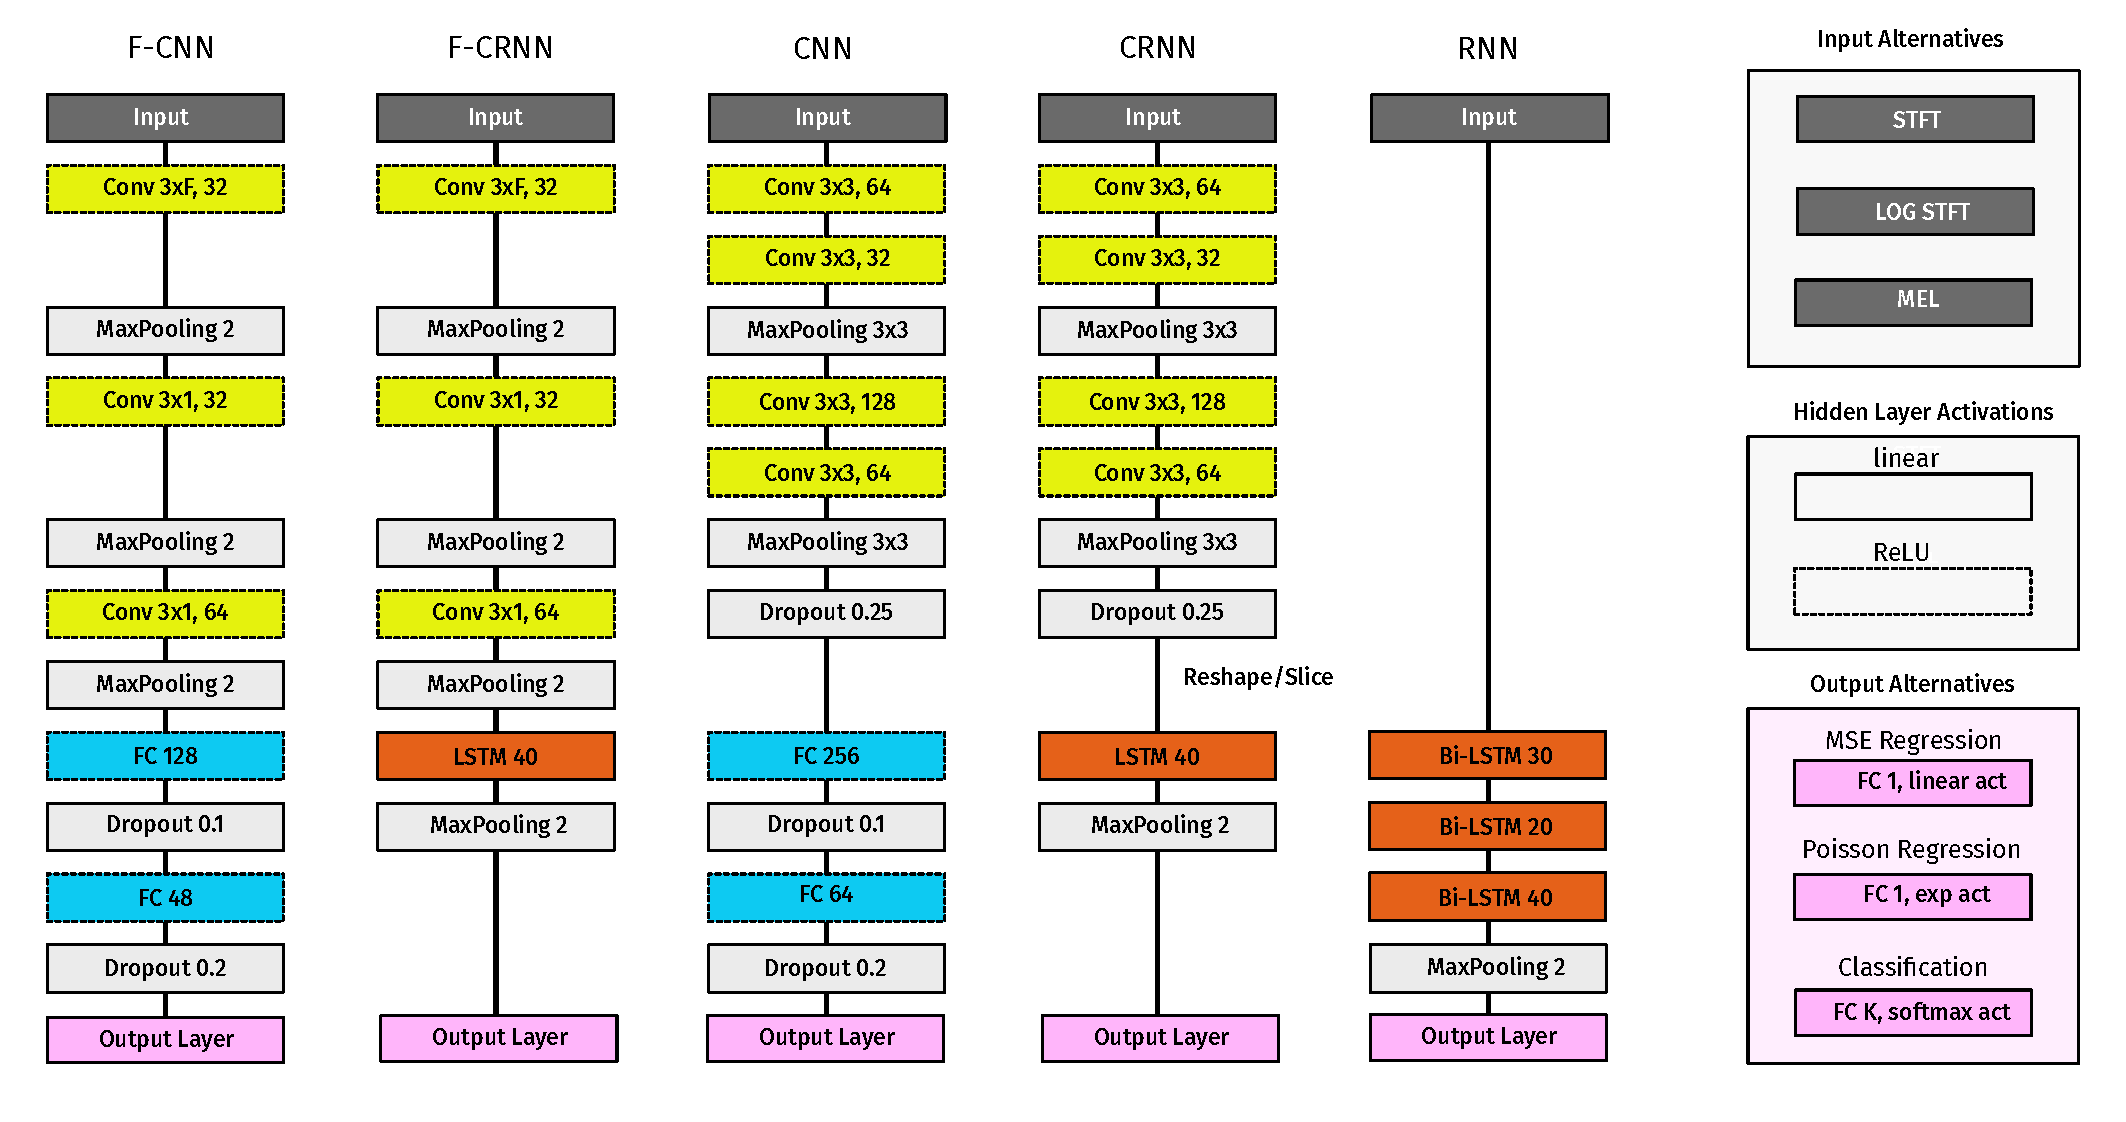
\includegraphics[width=0.9\textwidth]{Chapters/08_Analysis_CountNet/figures/networkoverview.pdf}
\caption{Overview of the proposed Architectures. \textsuperscript{\textregistered}2019 IEEE.}%
\label{fig:networkoverview}%
\end{figure*}

\subsection{Speech Corpora and Annotations}%
\label{ssec:corpus}
% * Libri Speech
% * Describe the used VAD
To date, many available speech datasets contain recordings where only a single speaker is active.
Datasets that include overlapped speech segments, either lack accurate annotations because the annotation of speech onsets and offsets in mixtures is cumbersome for humans or lack a controlled auditory environment such as in TV/broadcasting scenarios~\cite{Gravier12}.
Since a realistic dataset of fully overlapped speakers is not available, we chose to generate synthetic mixtures.
We recognize that in a simulated ``cocktail-party'' environment, mixtures lack the conversational aspect of human communication but provide a controlled environment which helps to understand how a DNN solves the count estimation problem.
As we aim for a speaker independent solution, we selected a speech corpus with preference to a high number of different speakers instead of the number of utterances, thus increasing the number of unique mixtures.
We selected \emph{LibriSpeech clean-360}\ \cite{panayotov15} which includes 363 hours of clean speech of English utterances from 921 speakers (439 female and 482 male speakers) sampled at 16 kHz.
% Compared to \emph{LibriSpeech}, \emph{TIMIT} is of lower recording quality and \emph{THCHS} represents mandarin speech.
% \par
% As revealed in Equation~\ref{eq:definition_k}, the maximum number of concurrent speakers \(cardinality\) requires annotation of the activity of each individual speaker.
% Even though many corpora come with word and phonemes annotation, they often are not consistent across different corpora.
% We therefore generated annotations based on a voice activity detection algorithm (VAD). As we rely on a robust VAD estimate, we found the implementation from the \emph{Chromium Web Browser} as part of the WebRTC Standard~\footnote{WebRTC 1.0: Real-time Communication Between Browsers W3C Editor's Draft 05 June 2017} to yield good results.
In the further course of this work (see Section~\ref{sec:evaluation}), we also present the results from test sets of two other datasets as listed in Table~\ref{tab:corpora}.
Furthermore, we included non-speech examples from the TUT Acoustic Scenes dataset~\cite{Mesaros16} in our training data to avoid using zero input samples for \(\cardinality = 0\) to increase the robustness against noise.

\begin{table}
  \centering
  \caption{Overview of speech corpora used in this work.}%
\label{tab:corpora}
\scriptsize
\begin{tabular}{llrrr}
  \toprule
  & & \multicolumn{3}{c}{Number of Speakers} \\
  \cmidrule(r){3-5}
  Name & Language &  Train & Valid. & Test\\
  \midrule
  LibriSpeech~\cite{panayotov15} & English & 921 & 40 & 40 \\
  TIMIT~\cite{TIMIT93} & English & 462 & 24 & 168 \\
  THCHS~\cite{THCHS15} & Mandarin & 30 & 10 & 10 \\
  \bottomrule
  \end{tabular}
\end{table}

\par
A single training tuple \( \left\{\mathbf{X}, k\right\} \) is generated by a synthetic speech mixture and their ground truth speaker count \(\cardinality \).
The mixtures are formed from random utterances of different speakers where silence in the beginning and end was removed to increase the overlap within one segment.
In fact, our method to generate synthetic samples results in an average overlap for \(k=2\) of 85\% and for \(k=10\) of 55\% (based on 5s segments).
This procedure is similar to~\cite{mesaros17} used to label the data.
Signals are mixed according to (\ref{eq:mixing_model}), peak normalized and then transformed to a time-frequency matrix \(X \in D \times F\).
Based on a voice activity detection algorithm (VAD), we used an implementation based on the WebRTC Standard~\cite{webrtc} where we computed the ground truth output \(\cardinality \) via (\ref{eq:definition_k}).
All samples are normalized to the average Euclidean norm of \(duration\) frames to be robust against gain variations as proposed by~\cite{uhlich15}.
Furthermore, the data was scaled to zero mean and unit standard deviation across the frequency dimension \(F\) over the full training data.
Scaling parameters were saved for validation and test.
For a more detailed description of the data set, the reader is referred to~\cite{stoeter17}.

% \subsubsection{Standardization, Normalization}%
% \label{ssec:norm}
%
% As our application more closely relates to source separation we want our trained DNN system to be robust against gain variations.
% We therefore find it important that the DNN can not leverage the gain factors of the mixture.
% We found that the averaged energy of one bin across \(duration\) already is a solid indicator for the number of speakers.
% In fact, in early experiments of the methods described in~\cite{sayoud10, andrei15} we were only able to reproduce their results when no normalization was applied.
% To accommodate these findings, we normalize \(\mathbf{X}\) to the average Euclidean norm of \(duration\) frames as proposed by~\cite{uhlich15}.
% Additionally, as common in machine learning, we scale the normalised input representation so that the feature dimension \(F\) have zero mean and unit variance/standard deviation across the whole training dataset (Standardization).

\subsection{Training Procedure}%
\label{ssec:parameters}
% * Optimizer
% other things
% To train each network we use Poisson sampling to balance the number of samples \(T_{ \cardinality}\) for each \(\cardinality \).
For all experiments we chose a medium sized training dataset of \(\cardinality \in \textrm{\{0, \ldots, 10\}}\) forming a total of \(T_{\textrm{train}} = 20.020\) mixtures  (1820 per \(k\)), each containing 10 seconds of audio, resulting in 55.55 hours of training material.
For each sample fed into the network, we select a random excerpt of duration \(D\) from each mixture. If not stated otherwise, \(D=5\)~seconds.
That way, for each epoch, the network is seeing slightly different samples, reducing the number of redundant samples and thus helping to speed up the stochastic gradient based training process.
\footnote{Note that for the validation and testing, excerpts are fixed.}
A similar training procedure is detailed in~\cite{schluter16, stoeter17}.
Each architecture is trained using the ADAM optimizer~\cite{kingma14} (learning rate: \(1 \cdot 10^{-3}\), \(\beta_1=0.9\), \(\beta_2=0.999\), \(\epsilon=1 \cdot 10^{-8}\)) using mini-batches of size 32.
Our training procedure verifies that all samples within a batch are from a different set of speakers.
In addition to the training dataset, we created a fully separated validation dataset of \(T_{\textrm{valid}} = 5720\) samples using a different set of speakers from \emph{LibriSpeech dev-clean}.
Early stopping (\(patience = 10\)) is applied by monitoring the validation loss to reduce the effect of overfitting.
Training never exceeded more than 50 epochs.
\par
We used the Keras~\cite{chollet15} framework and trained on multiple instances of Nvidia GTX 1080 GPUs.

\section{Model Selection}%
\label{sec:hyperparameters}

In this section, we evaluate three configurations of our proposed architectures, introduced in Section~\ref{sec:supervised_learning}.
Besides the architecture, we investigate different input representations as well as the three proposed output distributions (see Section~\ref{sec:problem_formulation}).
The goal of this is to determine the effect of these parameters and fix them to select a final trained network (model) based on these parameters.
\par
To allow for a controlled test environment and at the same time limit the number of training iterations, we fix certain parameters:
In this experiment, the level of the speakers was adjusted before mixing such that they have equal power.\@
Furthermore, the input duration \(D\) was fixed to five seconds.
For all experimental parameters, we repeated the training three times with different random seeds for each run and report averaged results to minimize random effects caused by early stopping.
We used the \emph{LibriSpeech} dataset for both training and validation and
performed evaluation of all models on \(T_{\textrm{test}} = 5720\) unique and unseen speaker mixtures from \emph{LibriSpeech test-clean} set with \(k_{\max} = 10\).
\par
Several well-established input representations were evaluated in~\cite{stoeter17} such as (linear or logarithmically scaled) \ac{STFT}, Mel filter bank outputs (MEL), Mel Frequency Cepstral Coefficients (MFCC) representations, typically chosen for speech applications (compare Table~\ref{tab:inputrep})

\begin{table}
  \centering
  \scriptsize
\begin{tabular}{rll}
\toprule
References & Task & Representation \\
\midrule
\cite{geiger13, hagerer17} & Overlap Detection/VAD & MFCC \\
\cite{Graves13, sainath15, marchi17} & ASR & MEL \\
\cite{amodei16} & ASR & \acs{STFT} \\
\cite{schluter15, schluter16} & Singing Voice AD & \(\log(1 + \mathbf{X})\) \\
\bottomrule
\end{tabular}
\caption{Speech related input representations in related work.}
\label{tab:inputrep}
\end{table}

Even though MFCCs are used in related tasks and are included in our baseline evaluations, they are known to perform poorly when used in CNNs~\cite{Seltzer13}.
This is why we decided to not to use the MFCCs as an input for the proposed architectures.
The remaining input representations are identical to those listed in~\cite{stoeter17}:

\noindent\textbf{1) STFT}: magnitude of the short-time Fourier transform computed using Hann-windows.
A frame length of \SI{25}{\milli\second} has been used.
The resulting input is \(X \in \mathbb{R}^{500 \times 201}\).\\
\textbf{2) STFTLOG}: logarithmically scaled magnitudes from \acs{STFT} representation using \(\log(1 + STFT)\).
The resulting input is \(X \in \mathbb{R}^{500 \times 201}\).\\
\textbf{3) MEL}: compute mapping from the \acs{STFT} output directly onto Mel basis using 40 triangular filters.
The resulting input is \(X \in \mathbb{R}^{500 \times 40}\).
\par
Before feature transformation, all input files were re-sampled to 16 kHz sampling rate. All features are computed using a hop size of \SI{10}{\milli\second}.

\subsection{Metric}%
\label{ssec:metrics}

Whereas the intermediate output \(y\) is treated as either a classification or a regression problem (see Section~\ref{sec:problem_formulation}) we evaluate the final output \(\cardinality \) as a discrete regression problem.
We, therefore, employ the mean absolute error (MAE) which is also commonly used for other count related tasks (c.f.~\cite{zhang15, Rezatofigh16}).
Since the MAE depends on the true count \(\cardinality \), we also present the MAE per class as:

\begin{equation}
  \mbox{MAE}(k) = \frac{1}{T_{\textrm{test}}} \sum_{t=1}^{T_\textrm{test}}\left| \hat{k} - k \right|.
\end{equation}

which is then averaged across the classes, i.e.,

\begin{equation}
  \mbox{MAE} = \frac{1}{k_{\max}} \sum_{k=0}^{k_{\max}} \mbox{MAE}(k).
\end{equation}

\subsection{Model Comparison}%
\label{ssec:model_comparsion}

\begin{figure*}
\centering
\subcaptionbox[by feature representations.]{%
    by feature representations.%
    \label{fig:ssec:exp_fixed_gains/A}%
}
[\textwidth]{% This file was created by matplotlib2tikz v0.6.13.
\begin{tikzpicture}

% colors from colorbrewer Set3
\definecolor{color0}{rgb}{0.917647058823529,0.917647058823529,0.949019607843137}
\definecolor{color1}{RGB}{191,91,23}
\definecolor{color3}{RGB}{190,174,212}
\definecolor{color2}{RGB}{253,192,134}

\begin{axis}[
xlabel={k},
ylabel={MAE},
width=0.66\textwidth,
height=0.5\textwidth,
xmin=-0.5, xmax=10.5,
ymin=-0.05, ymax=0.9,
ytick={-0.1,0,0.1,0.2,0.3,0.4,0.5,0.6,0.7,0.8,0.9},
yticklabels={0.0,0.0,0.1,0.2,0.3,0.4,0.5,0.6,0.7,0.8,0.9},
xtick distance=1,
tick align=outside,
tick pos=left,
ymajorgrids,
xmajorgrids,
grid style={line width=.1pt, draw=gray!20},
major grid style={line width=.2pt,draw=gray!20},
axis line style={black},
legend style={at={(0.03,0.97)}, anchor=north west, draw=none, fill==gray!0, font=\scriptsize},
legend cell align={left},
legend entries={{MEL40},{STFT},{STFTLOG}}
]
\addplot [only marks, draw=color1, fill=color1, colormap/blackwhite]
table{%
x                      y
-3.750000000000001e-02 +1.282051285115891e-03
+9.625000000000000e-01 +4.378956559182671e-02
+1.962500000000000e+00 +1.698966412812240e-01
+2.962500000000000e+00 +2.904593644946708e-01
+3.962500000000000e+00 +3.819121458168999e-01
+4.962500000000000e+00 +5.342699044052212e-01
+5.962500000000000e+00 +6.399449048893949e-01
+6.962500000000000e+00 +7.022138688498571e-01
+7.962500000000000e+00 +6.717410322614437e-01
+8.962500000000000e+00 +6.421099899821276e-01
+9.962500000000000e+00 +7.441498321916922e-01
};
\addplot [line width=2.00pt, color1, forget plot]
table {%
-0.0375 0.00128205128511589
0.9625 0.0437895655918267
1.9625 0.169896641281224
2.9625 0.290459364494671
3.9625 0.3819121458169
4.9625 0.534269904405221
5.9625 0.639944904889395
6.9625 0.702213868849857
7.9625 0.671741032261444
8.9625 0.642109989982128
9.9625 0.744149832191692
};
\addplot [line width=2.00pt, color1, forget plot]
table {%
-0.0375 0.0002991452993443
-0.0375 0.00290598291171611
};
\addplot [line width=2.00pt, color1, forget plot]
table {%
0.9625 0.0292021391029433
0.9625 0.0628356254969424
};
\addplot [line width=2.00pt, color1, forget plot]
table {%
1.9625 0.148319336806491
1.9625 0.1932881148387
};
\addplot [line width=2.00pt, color1, forget plot]
table {%
2.9625 0.260852964485001
2.9625 0.322079899352019
};
\addplot [line width=2.00pt, color1, forget plot]
table {%
3.9625 0.348403317338685
3.9625 0.418488374525981
};
\addplot [line width=2.00pt, color1, forget plot]
table {%
4.9625 0.490396980724153
4.9625 0.580383148183019
};
\addplot [line width=2.00pt, color1, forget plot]
table {%
5.9625 0.59489899164649
5.9625 0.690870064470585
};
\addplot [line width=2.00pt, color1, forget plot]
table {%
6.9625 0.654216791062228
6.9625 0.75059524217121
};
\addplot [line width=2.00pt, color1, forget plot]
table {%
7.9625 0.629482719495514
7.9625 0.712939632123146
};
\addplot [line width=2.00pt, color1, forget plot]
table {%
8.9625 0.5712637464472
8.9625 0.720740745223197
};
\addplot [line width=2.00pt, color1, forget plot]
table {%
9.9625 0.603217593893058
9.9625 0.889956860029537
};
\addplot [only marks, draw=color2, fill=color2, colormap/blackwhite]
table{%
x                      y
+0.000000000000000e+00 +4.017094149429383e-03
+1.000000000000000e+00 +2.165466058294658e-02
+2.000000000000000e+00 +1.097760553809459e-01
+3.000000000000000e+00 +2.075775420503098e-01
+4.000000000000000e+00 +3.075366057808496e-01
+5.000000000000000e+00 +4.309067676908769e-01
+6.000000000000000e+00 +5.230027550672368e-01
+7.000000000000000e+00 +6.100250622981175e-01
+8.000000000000000e+00 +5.915135611073551e-01
+9.000000000000000e+00 +5.562738505022561e-01
+1.000000000000000e+01 +6.068181814770105e-01
};
\addplot [line width=2.00pt, color2, forget plot]
table {%
0 0.00401709414942938
1 0.0216546605829466
2 0.109776055380946
3 0.20757754205031
4 0.30753660578085
5 0.430906767690877
6 0.523002755067237
7 0.610025062298117
8 0.591513561107355
9 0.556273850502256
10 0.60681818147701
};
\addplot [line width=2.00pt, color2, forget plot]
table {%
0 0.00141025642932265
0 0.00777884649395501
};
\addplot [line width=2.00pt, color2, forget plot]
table {%
1 0.015104780559566
1 0.0292981881977767
};
\addplot [line width=2.00pt, color2, forget plot]
table {%
2 0.0935389754212398
2 0.126616063651554
};
\addplot [line width=2.00pt, color2, forget plot]
table {%
3 0.184214762288727
3 0.232517668003831
};
\addplot [line width=2.00pt, color2, forget plot]
table {%
4 0.283712317184782
4 0.329804048656288
};
\addplot [line width=2.00pt, color2, forget plot]
table {%
5 0.401557044723647
5 0.465348019600485
};
\addplot [line width=2.00pt, color2, forget plot]
table {%
6 0.490907942142724
6 0.554963269541031
};
\addplot [line width=2.00pt, color2, forget plot]
table {%
7 0.571706349037544
7 0.650759191716972
};
\addplot [line width=2.00pt, color2, forget plot]
table {%
8 0.557388451102525
8 0.628085083916509
};
\addplot [line width=2.00pt, color2, forget plot]
table {%
9 0.510563413293006
9 0.60849158311509
};
\addplot [line width=2.00pt, color2, forget plot]
table {%
10 0.507567340790322
10 0.711869740708408
};
\path [draw=white, fill opacity=0] (axis cs:0,-0.0552693502854651)
--(axis cs:0,0.934967631949299);

\path [draw=white, fill opacity=0] (axis cs:1,-0.0552693502854651)
--(axis cs:1,0.934967631949299);

\path [draw=white, fill opacity=0] (axis cs:-0.5,0)
--(axis cs:10.5,0);

\path [draw=white, fill opacity=0] (axis cs:-0.5,1)
--(axis cs:10.5,1);

\addplot [only marks, draw=color3, fill=color3, colormap/blackwhite]
table{%
x                      y
+3.750000000000001e-02 +4.491453003381084e-02
+1.037500000000000e+00 +4.894127914890618e-02
+2.037500000000000e+00 +1.479328153983824e-01
+3.037500000000000e+00 +2.669022376087070e-01
+4.037500000000000e+00 +3.958656320969263e-01
+5.037500000000000e+00 +5.179225227638933e-01
+6.037500000000000e+00 +6.520202012977215e-01
+7.037500000000000e+00 +7.256892264536648e-01
+8.037500000000000e+00 +6.448818897898534e-01
+9.037500000000000e+00 +5.645342315434071e-01
+1.003750000000000e+01 +5.662037049329240e-01
};
\addplot [line width=2.00pt, color3, forget plot]
table {%
0.0375 0.0449145300338108
1.0375 0.0489412791489062
2.0375 0.147932815398382
3.0375 0.266902237608707
4.0375 0.395865632096926
5.0375 0.517922522763893
6.0375 0.652020201297722
7.0375 0.725689226453665
8.0375 0.644881889789853
9.0375 0.564534231543407
10.0375 0.566203704932924
};
\addplot [line width=2.00pt, color3, forget plot]
table {%
0.0375 0.00563675216719425
0.0375 0.0978333334729233
};
\addplot [line width=2.00pt, color3, forget plot]
table {%
1.0375 0.0240973587901605
1.0375 0.083095393889988
};
\addplot [line width=2.00pt, color3, forget plot]
table {%
2.0375 0.119852497411666
2.0375 0.180880703087784
};
\addplot [line width=2.00pt, color3, forget plot]
table {%
3.0375 0.236119944983176
3.0375 0.298233213870577
};
\addplot [line width=2.00pt, color3, forget plot]
table {%
4.0375 0.354053618227044
4.0375 0.434679154426463
};
\addplot [line width=2.00pt, color3, forget plot]
table {%
5.0375 0.46628033370452
5.0375 0.5704150723004
};
\addplot [line width=2.00pt, color3, forget plot]
table {%
6.0375 0.599070247832217
6.0375 0.705386820743399
};
\addplot [line width=2.00pt, color3, forget plot]
table {%
7.0375 0.663815792690194
7.0375 0.786649962138935
};
\addplot [line width=2.00pt, color3, forget plot]
table {%
8.0375 0.588227250151147
8.0375 0.700395887889496
};
\addplot [line width=2.00pt, color3, forget plot]
table {%
9.0375 0.508768798929406
9.0375 0.623634119981668
};
\addplot [line width=2.00pt, color3, forget plot]
table {%
10.0375 0.464126683435331
10.0375 0.659747474216276
};
\end{axis}

\end{tikzpicture}
}%
\hspace{0.2\textwidth} % seperation
\subcaptionbox[by output distribution.]{%
    by output distribution.%
    \label{fig:ssec:exp_fixed_gains/B}%
}
[\textwidth]{% This file was created by matplotlib2tikz v0.6.13.
\begin{tikzpicture}

\definecolor{color0}{rgb}{0.917647058823529,0.917647058823529,0.949019607843137}
\definecolor{color1}{RGB}{102,194,165}
\definecolor{color3}{RGB}{252,141,98}
\definecolor{color2}{RGB}{141,160,203}

\begin{axis}[
xlabel={k},
ylabel={MAE},
width=0.66\textwidth,
height=0.5\textwidth,
xmin=-0.5, xmax=10.5,
ymin=-0.05, ymax=0.9,
ytick={-0.1,0,0.1,0.2,0.3,0.4,0.5,0.6,0.7,0.8,0.9},
yticklabels={0.0,0.0,0.1,0.2,0.3,0.4,0.5,0.6,0.7,0.8,0.9},
xtick distance=1,
tick align=outside,
tick pos=left,
ymajorgrids,
xmajorgrids,
axis line style={black},
grid style={line width=.1pt, draw=gray!20},
major grid style={line width=.2pt,draw=gray!20},
legend style={at={(0.03,0.97)}, anchor=north west, draw=none, fill==gray!0, font=\scriptsize},
legend entries={{Classification},{Gaussian Regr.},{Poisson Regr.}},
legend cell align={left}
]
\addplot [only marks, draw=color1, fill=color1, colormap/blackwhite]
table{%
x                      y
-3.750000000000001e-02 +3.735042735042735e-02
+9.625000000000000e-01 +2.086880593756822e-02
+1.962500000000000e+00 +9.780361757105942e-02
+2.962500000000000e+00 +2.061248527679623e-01
+3.962500000000000e+00 +3.319121447028424e-01
+4.962500000000000e+00 +4.427415921668795e-01
+5.962500000000000e+00 +5.417355371900826e-01
+6.962500000000000e+00 +6.838345864661655e-01
+7.962500000000000e+00 +7.204724409448819e-01
+8.962500000000000e+00 +7.120987654320987e-01
+9.962500000000000e+00 +3.478956228956228e-01
};
\addplot [line width=2.00pt, color1, forget plot]
table {%
-0.0375 0.0373504273504274
0.9625 0.0208688059375682
1.9625 0.0978036175710594
2.9625 0.206124852767962
3.9625 0.331912144702842
4.9625 0.44274159216688
5.9625 0.541735537190083
6.9625 0.683834586466165
7.9625 0.720472440944882
8.9625 0.712098765432099
9.9625 0.347895622895623
};
\addplot [line width=2.00pt, color1, forget plot]
table {%
-0.0375 0.00153739316239316
-0.0375 0.0895363247863248
};
\addplot [line width=2.00pt, color1, forget plot]
table {%
0.9625 0.0127919668194717
0.9625 0.0316961362148003
};
\addplot [line width=2.00pt, color1, forget plot]
table {%
1.9625 0.0817797157622739
1.9625 0.114736218776916
};
\addplot [line width=2.00pt, color1, forget plot]
table {%
2.9625 0.182602080879466
2.9625 0.231887514723204
};
\addplot [line width=2.00pt, color1, forget plot]
table {%
3.9625 0.29969315245478
3.9625 0.365779500430663
};
\addplot [line width=2.00pt, color1, forget plot]
table {%
4.9625 0.399341209025117
4.9625 0.485740740740741
};
\addplot [line width=2.00pt, color1, forget plot]
table {%
5.9625 0.502793847566575
5.9625 0.579757805325987
};
\addplot [line width=2.00pt, color1, forget plot]
table {%
6.9625 0.631313700918964
6.9625 0.745908521303258
};
\addplot [line width=2.00pt, color1, forget plot]
table {%
7.9625 0.66682195975503
7.9625 0.773801399825022
};
\addplot [line width=2.00pt, color1, forget plot]
table {%
8.9625 0.663826038159372
8.9625 0.758792368125701
};
\addplot [line width=2.00pt, color1, forget plot]
table {%
9.9625 0.283256523569024
9.9625 0.418800505050505
};
\addplot [only marks, draw=color2, fill=color2, colormap/blackwhite]
table{%
x                      y
+0.000000000000000e+00 +1.235042760510825e-02
+1.000000000000000e+00 +7.290984498750833e-02
+2.000000000000000e+00 +1.817398789856169e-01
+3.000000000000000e+00 +2.903023165133264e-01
+4.000000000000000e+00 +3.893195516533322e-01
+5.000000000000000e+00 +5.250319321950276e-01
+6.000000000000000e+00 +6.450872368282742e-01
+7.000000000000000e+00 +6.927318334579468e-01
+8.000000000000000e+00 +6.023184604114956e-01
+9.000000000000000e+00 +5.145679036776225e-01
+1.000000000000000e+01 +7.327020216319297e-01
};
\addplot [line width=2.00pt, color2, forget plot]
table {%
0 0.0123504276051083
1 0.0729098449875083
2 0.181739878985617
3 0.290302316513326
4 0.389319551653332
5 0.525031932195028
6 0.645087236828274
7 0.692731833457947
8 0.602318460411496
9 0.514567903677623
10 0.73270202163193
};
\addplot [line width=2.00pt, color2, forget plot]
table {%
0 0.00534081213764795
0 0.0241025645566535
};
\addplot [line width=2.00pt, color2, forget plot]
table {%
1 0.0466262830175563
1 0.110413665477342
};
\addplot [line width=2.00pt, color2, forget plot]
table {%
2 0.155333763578286
2 0.211202626282142
};
\addplot [line width=2.00pt, color2, forget plot]
table {%
3 0.257034745460583
3 0.324860619132717
};
\addplot [line width=2.00pt, color2, forget plot]
table {%
4 0.34692829568353
4 0.432953272768193
};
\addplot [line width=2.00pt, color2, forget plot]
table {%
5 0.478991059346331
5 0.574425296684106
};
\addplot [line width=2.00pt, color2, forget plot]
table {%
6 0.590747243298425
6 0.699374426702658
};
\addplot [line width=2.00pt, color2, forget plot]
table {%
7 0.634959278139803
7 0.754830837696791
};
\addplot [line width=2.00pt, color2, forget plot]
table {%
8 0.562505469305648
8 0.6433584856987
};
\addplot [line width=2.00pt, color2, forget plot]
table {%
9 0.468725030223529
9 0.570103260063463
};
\addplot [line width=2.00pt, color2, forget plot]
table {%
10 0.624493893070353
10 0.840917507157558
};
% \path [draw=white, fill opacity=0] (axis cs:0,-0.0600185928210457)
% --(axis cs:0,1.00006922752411);
%
% \path [draw=white, fill opacity=0] (axis cs:1,-0.0600185928210457)
% --(axis cs:1,1.00006922752411);
%
% \path [draw=white, fill opacity=0] (axis cs:-0.5,0)
% --(axis cs:10.5,0);
%
% \path [draw=white, fill opacity=0] (axis cs:-0.5,1)
% --(axis cs:10.5,1);

\addplot [only marks, draw=color3, fill=color3, colormap/blackwhite]
table{%
x                      y
+3.750000000000001e-02 +5.128205128205128e-04
+1.037500000000000e+00 +2.060685439860293e-02
+2.037500000000000e+00 +1.480620155038760e-01
+3.037500000000000e+00 +2.685119748723989e-01
+4.037500000000000e+00 +3.640826873385014e-01
+5.037500000000000e+00 +5.153256704980842e-01
+6.037500000000000e+00 +6.281450872359963e-01
+7.037500000000000e+00 +6.613617376775270e-01
+8.037500000000000e+00 +5.853455818022747e-01
+9.037500000000000e+00 +5.362514029180696e-01
+1.003750000000000e+01 +8.365740740740741e-01
};
\addplot [line width=2.00pt, color3, forget plot]
table {%
0.0375 0.000512820512820513
1.0375 0.0206068543986029
2.0375 0.148062015503876
3.0375 0.268511974872399
4.0375 0.364082687338501
5.0375 0.515325670498084
6.0375 0.628145087235996
7.0375 0.661361737677527
8.0375 0.585345581802275
9.0375 0.53625140291807
10.0375 0.836574074074074
};
\addplot [line width=2.00pt, color3, forget plot]
table {%
0.0375 0.000170940170940171
0.0375 0.000982905982905983
};
\addplot [line width=2.00pt, color3, forget plot]
table {%
1.0375 0.0122647893473041
1.0375 0.0345797860729098
};
\addplot [line width=2.00pt, color3, forget plot]
table {%
2.0375 0.12656976744186
2.0375 0.169559646856158
};
\addplot [line width=2.00pt, color3, forget plot]
table {%
3.0375 0.240591872791519
3.0375 0.298862387122104
};
\addplot [line width=2.00pt, color3, forget plot]
table {%
4.0375 0.332558139534884
4.0375 0.39405684754522
};
\addplot [line width=2.00pt, color3, forget plot]
table {%
5.0375 0.476749680715198
5.0375 0.554259259259259
};
\addplot [line width=2.00pt, color3, forget plot]
table {%
6.0375 0.587143021120294
6.0375 0.676090449954086
};
\addplot [line width=2.00pt, color3, forget plot]
table {%
7.0375 0.614816207184628
7.0375 0.704314954051796
};
\addplot [line width=2.00pt, color3, forget plot]
table {%
8.0375 0.549119641294838
8.0375 0.623103674540682
};
\addplot [line width=2.00pt, color3, forget plot]
table {%
9.0375 0.475597081930415
9.0375 0.597627384960718
};
\addplot [line width=2.00pt, color3, forget plot]
table {%
10.0375 0.727001262626263
10.0375 0.951883417508417
};
\end{axis}

\end{tikzpicture}
}%
\hspace{0.2\textwidth} % seperation
\subcaptionbox[by feature representations.]{%
    by feature representations.%
    \label{fig:ssec:exp_fixed_gains/C}%
}
[\textwidth]{% This file was created by matplotlib2tikz v0.6.13.
\begin{tikzpicture}

\definecolor{color0}{rgb}{0.917647058823529,0.917647058823529,0.949019607843137}

\begin{axis}[
xlabel={k},
ylabel={MAE},
width=0.66\textwidth,
height=0.5\textwidth,
xmin=-0.5, xmax=10.5,
ymin=-0.05, ymax=0.9,
ytick={-0.1,0,0.1,0.2,0.3,0.4,0.5,0.6,0.7,0.8,0.9},
yticklabels={0.0,0.0,0.1,0.2,0.3,0.4,0.5,0.6,0.7,0.8,0.9},
xtick distance=1,
tick align=outside,
tick pos=left,
ymajorgrids,
xmajorgrids,
axis line style={black},
grid style={line width=.1pt, draw=gray!20},
major grid style={line width=.2pt,draw=gray!20},
legend entries={{F-CNN},{CNN},{F-CRNN},{CRNN},{RNN~\cite{stoeter17}}},
legend style={at={(0.03,0.97)}, anchor=north west, draw=none, fill=gray!0},
legend cell align={left}
]
\addplot [only marks, draw=FCNN, fill=FCNN, colormap/blackwhite]
table{%
x                      y
-6.250000000000000e-02 +1.609686645533242e-02
+9.375000000000000e-01 +6.810740004287860e-02
+1.937500000000000e+00 +1.871231682694852e-01
+2.937500000000000e+00 +2.900143965558066e-01
+3.937500000000000e+00 +4.082687340469289e-01
+4.937500000000000e+00 +5.654179110829165e-01
+5.937500000000000e+00 +6.553412880013030e-01
+6.937500000000000e+00 +7.385129500517637e-01
+7.937500000000000e+00 +6.676144655364774e-01
+8.937500000000000e+00 +6.725028088197162e-01
+9.937500000000000e+00 +8.343855208151804e-01
};
\addplot [line width=2.00pt, FCNN, forget plot]
table {%
-0.0625 0.0160968664553324
0.9375 0.0681074000428786
1.9375 0.187123168269485
2.9375 0.290014396555807
3.9375 0.408268734046929
4.9375 0.565417911082917
5.9375 0.655341288001303
6.9375 0.738512950051764
7.9375 0.667614465536477
8.9375 0.672502808819716
9.9375 0.83438552081518
};
\addplot [line width=2.00pt, FCNN, forget plot]
table {%
-0.0625 0.00427350433559245
-0.0625 0.032419872278337
};
\addplot [line width=2.00pt, FCNN, forget plot]
table {%
0.9375 0.0406734335280436
0.9375 0.10157898504591
};
\addplot [line width=2.00pt, FCNN, forget plot]
table {%
1.9375 0.149366565919747
1.9375 0.233137736180939
};
\addplot [line width=2.00pt, FCNN, forget plot]
table {%
2.9375 0.254217380758762
2.9375 0.327314815066483
};
\addplot [line width=2.00pt, FCNN, forget plot]
table {%
3.9375 0.374671620453119
3.9375 0.445592879322353
};
\addplot [line width=2.00pt, FCNN, forget plot]
table {%
4.9375 0.520718039641279
4.9375 0.61367780890385
};
\addplot [line width=2.00pt, FCNN, forget plot]
table {%
5.9375 0.600531829466213
5.9375 0.715734995382986
};
\addplot [line width=2.00pt, FCNN, forget plot]
table {%
6.9375 0.673544972183909
6.9375 0.808347258480503
};
\addplot [line width=2.00pt, FCNN, forget plot]
table {%
7.9375 0.600100245278955
7.9375 0.744099954962643
};
\addplot [line width=2.00pt, FCNN, forget plot]
table {%
8.9375 0.585170224673887
8.9375 0.760961468631839
};
\addplot [line width=2.00pt, FCNN, forget plot]
table {%
9.9375 0.656660354222713
9.9375 1.02770763036244
};
\addplot [only marks, draw=CNN, fill=CNN, colormap/blackwhite]
table{%
x                      y
-3.125000000000000e-02 +1.495726509789201e-03
+9.687500000000000e-01 +1.760896459410368e-02
+1.968750000000000e+00 +1.216623599392619e-01
+2.968750000000000e+00 +2.069100901482539e-01
+3.968750000000000e+00 +2.922049940205702e-01
+4.968750000000000e+00 +4.167730962238836e-01
+5.968750000000000e+00 +5.557086000319903e-01
+6.968750000000000e+00 +5.869534927485414e-01
+7.968750000000000e+00 +5.456401261879356e-01
+8.968750000000000e+00 +5.296670419778263e-01
+9.968750000000000e+00 +6.469556705317513e-01
};
\addplot [line width=2.00pt, CNN, forget plot]
table {%
-0.03125 0.0014957265097892
0.96875 0.0176089645941037
1.96875 0.121662359939262
2.96875 0.206910090148254
3.96875 0.29220499402057
4.96875 0.416773096223884
5.96875 0.55570860003199
6.96875 0.586953492748541
7.96875 0.545640126187936
8.96875 0.529667041977826
9.96875 0.646955670531751
};
\addplot [line width=2.00pt, CNN, forget plot]
table {%
-0.03125 0.000569800578609661
-0.03125 0.00242343307596477
};
\addplot [line width=2.00pt, CNN, forget plot]
table {%
0.96875 0.0108382449495332
0.96875 0.0252510370163853
};
\addplot [line width=2.00pt, CNN, forget plot]
table {%
1.96875 0.0968938411976859
1.96875 0.149162000738605
};
\addplot [line width=2.00pt, CNN, forget plot]
table {%
2.96875 0.172551041119997
2.96875 0.243168432323684
};
\addplot [line width=2.00pt, CNN, forget plot]
table {%
3.96875 0.253718057931103
3.96875 0.335432813824626
};
\addplot [line width=2.00pt, CNN, forget plot]
table {%
4.96875 0.357010075388622
4.96875 0.480567972900403
};
\addplot [line width=2.00pt, CNN, forget plot]
table {%
5.96875 0.49686065282448
5.96875 0.629650670435721
};
\addplot [line width=2.00pt, CNN, forget plot]
table {%
6.96875 0.520739347236638
6.96875 0.652126840199934
};
\addplot [line width=2.00pt, CNN, forget plot]
table {%
7.96875 0.500136699940119
7.96875 0.588074144240187
};
\addplot [line width=2.00pt, CNN, forget plot]
table {%
8.96875 0.475188928860774
8.96875 0.57882903330265
};
\addplot [line width=2.00pt, CNN, forget plot]
table {%
9.96875 0.499768520983649
9.96875 0.791559695281866
};
\path [draw=white, fill opacity=0] (axis cs:0,-0.0642762651515782)
--(axis cs:0,1.07970686348216);

\path [draw=white, fill opacity=0] (axis cs:1,-0.0642762651515782)
--(axis cs:1,1.07970686348216);

\path [draw=white, fill opacity=0] (axis cs:-0.5,0)
--(axis cs:10.5,0);

\path [draw=white, fill opacity=0] (axis cs:-0.5,1)
--(axis cs:10.5,1);

\addplot [only marks, draw=FCRNN, fill=FCRNN, colormap/blackwhite]
table{%
x                      y
+0.000000000000000e+00 +6.346153848163752e-02
+1.000000000000000e+00 +7.218220163694986e-02
+2.000000000000000e+00 +1.653028996578414e-01
+3.000000000000000e+00 +2.925664174269669e-01
+4.000000000000000e+00 +4.153029006632313e-01
+5.000000000000000e+00 +5.485312881513033e-01
+6.000000000000000e+00 +6.603152773086178e-01
+7.000000000000000e+00 +7.562656681606015e-01
+8.000000000000000e+00 +6.770195411537229e-01
+9.000000000000000e+00 +5.510662176793674e-01
+1.000000000000000e+01 +6.087962971993969e-01
};
\addplot [line width=2.00pt, FCRNN, forget plot]
table {%
0 0.0634615384816375
1 0.0721822016369499
2 0.165302899657841
3 0.292566417426967
4 0.415302900663231
5 0.548531288151303
6 0.660315277308618
7 0.756265668160601
8 0.677019541153723
9 0.551066217679367
10 0.608796297199397
};
\addplot [line width=2.00pt, FCRNN, forget plot]
table {%
0 0.00327457266575969
0 0.152783119675935
};
\addplot [line width=2.00pt, FCRNN, forget plot]
table {%
1 0.0379811538036914
1 0.117306993108207
};
\addplot [line width=2.00pt, FCRNN, forget plot]
table {%
2 0.142825868812946
2 0.189570772423677
};
\addplot [line width=2.00pt, FCRNN, forget plot]
table {%
3 0.26108166456477
3 0.321173601928928
};
\addplot [line width=2.00pt, FCRNN, forget plot]
table {%
4 0.379186404986292
4 0.450771608875335
};
\addplot [line width=2.00pt, FCRNN, forget plot]
table {%
5 0.503400382091471
5 0.592736270459379
};
\addplot [line width=2.00pt, FCRNN, forget plot]
table {%
6 0.610785893782549
6 0.711432509583583
};
\addplot [line width=2.00pt, FCRNN, forget plot]
table {%
7 0.707322127606271
7 0.805423287159302
};
\addplot [line width=2.00pt, FCRNN, forget plot]
table {%
8 0.627726745471189
8 0.733316930837779
};
\addplot [line width=2.00pt, FCRNN, forget plot]
table {%
9 0.488881408392023
9 0.614322857952468
};
\addplot [line width=2.00pt, FCRNN, forget plot]
table {%
10 0.498625141462493
10 0.723000841983307
};
\addplot [only marks, draw=CRNN, fill=CRNN, colormap/blackwhite]
table{%
x                      y
+3.125000000000000e-02 +1.424501451631833e-03
+1.031250000000000e+00 +7.567488835640818e-03
+2.031250000000000e+00 +7.493540085798669e-02
+3.031250000000000e+00 +1.739301140378820e-01
+4.031250000000000e+00 +2.658627627782701e-01
+5.031250000000000e+00 +3.860508020218169e-01
+6.031250000000000e+00 +5.054331182119932e-01
+7.031250000000000e+00 +5.913394604825403e-01
+8.031250000000000e+00 +5.926655008150419e-01
+9.031250000000000e+00 +4.832023948219176e-01
+1.003125000000000e+01 +3.981481475209950e-01
};
\addplot [line width=2.00pt, CRNN, forget plot]
table {%
0.03125 0.00142450145163183
1.03125 0.00756748883564082
2.03125 0.0749354008579867
3.03125 0.173930114037882
4.03125 0.26586276277827
5.03125 0.386050802021817
6.03125 0.505433118211993
7.03125 0.59133946048254
8.03125 0.592665500815042
9.03125 0.483202394821918
10.03125 0.398148147520995
};
\addplot [line width=2.00pt, CRNN, forget plot]
table {%
0.03125 0.0004985754989735
0.03125 0.00270655276526948
};
\addplot [line width=2.00pt, CRNN, forget plot]
table {%
1.03125 0.00203558178730112
1.03125 0.0145546822128031
};
\addplot [line width=2.00pt, CRNN, forget plot]
table {%
2.03125 0.0569157335567367
2.03125 0.0955408415482242
};
\addplot [line width=2.00pt, CRNN, forget plot]
table {%
3.03125 0.146104894003063
3.03125 0.204166667151622
};
\addplot [line width=2.00pt, CRNN, forget plot]
table {%
4.03125 0.23291343713199
4.03125 0.2977354312345
};
\addplot [line width=2.00pt, CRNN, forget plot]
table {%
5.03125 0.348859443451997
5.03125 0.421471903264116
};
\addplot [line width=2.00pt, CRNN, forget plot]
table {%
6.03125 0.457526017299231
6.03125 0.55380509473705
};
\addplot [line width=2.00pt, CRNN, forget plot]
table {%
7.03125 0.533848510757068
7.03125 0.653164161347108
};
\addplot [line width=2.00pt, CRNN, forget plot]
table {%
8.03125 0.543070136671617
8.03125 0.643294327571819
};
\addplot [line width=2.00pt, CRNN, forget plot]
table {%
9.03125 0.423866442182048
9.03125 0.545838009867325
};
\addplot [line width=2.00pt, CRNN, forget plot]
table {%
10.03125 0.310530652987377
10.03125 0.493304572760114
};
\addplot [only marks, draw=RNN, fill=RNN, colormap/blackwhite]
table{%
x                      y
+6.250000000000000e-02 +1.210826215535890e-03
+1.062500000000000e+00 +2.517645376322615e-02
+2.062500000000000e+00 +1.636520247096787e-01
+3.062500000000000e+00 +3.114775554205700e-01
+4.062500000000000e+00 +4.272179146487926e-01
+5.062500000000000e+00 +5.550588939533989e-01
+6.062500000000000e+00 +6.481481518700176e-01
+7.062500000000000e+00 +7.234753578926187e-01
+8.062500000000000e+00 +6.972878382379093e-01
+9.062500000000000e+00 +7.017583234141570e-01
+1.006250000000000e+01 +7.070005616020540e-01
};
\addplot [line width=2.00pt, RNN, forget plot]
table {%
0.0625 0.00121082621553589
1.0625 0.0251764537632262
2.0625 0.163652024709679
3.0625 0.31147755542057
4.0625 0.427217914648793
5.0625 0.555058893953399
6.0625 0.648148151870018
7.0625 0.723475357892619
8.0625 0.697287838237909
9.0625 0.701758323414157
10.0625 0.707000561602054
};
\addplot [line width=2.00pt, RNN, forget plot]
table {%
0.0625 0.000498575503043061
0.0625 0.00206552708364109
};
\addplot [line width=2.00pt, RNN, forget plot]
table {%
1.0625 0.0152059230939088
1.0625 0.0382776697341815
};
\addplot [line width=2.00pt, RNN, forget plot]
table {%
2.0625 0.137376184544189
2.0625 0.190929156405883
};
\addplot [line width=2.00pt, RNN, forget plot]
table {%
3.0625 0.277707434068703
3.0625 0.350161955888962
};
\addplot [line width=2.00pt, RNN, forget plot]
table {%
4.0625 0.388874532062664
4.0625 0.477535531107479
};
\addplot [line width=2.00pt, RNN, forget plot]
table {%
5.0625 0.501489998066643
5.0625 0.623877187503222
};
\addplot [line width=2.00pt, RNN, forget plot]
table {%
6.0625 0.591823541416117
6.0625 0.716944064002884
};
\addplot [line width=2.00pt, RNN, forget plot]
table {%
7.0625 0.666513509922657
7.0625 0.78691347012718
};
\addplot [line width=2.00pt, RNN, forget plot]
table {%
8.0625 0.642745697520484
8.0625 0.764656240344221
};
\addplot [line width=2.00pt, RNN, forget plot]
table {%
9.0625 0.624979422747464
9.0625 0.786464645104532
};
\addplot [line width=2.00pt, RNN, forget plot]
table {%
10.0625 0.566563200983234
10.0625 0.853794893655846
};
\end{axis}

\end{tikzpicture}
}%
\caption[Short Caption]{Figure shows results of average mean absolute error (MAE) on mixtures of speakers with equal power as described in \textsc{Section~\ref{ssec:model_comparsion}} per ground truth count \(k=[0\ldots10]\). Error bars show the 95\% confidence intervals. Results in (a) are averaged over factors shown in (b) and (c) and similarly for (b) and (c). \textsuperscript{\textregistered}2019 IEEE.}
\label{fig:fixed-gain-results}
\end{figure*}

To find the best parameters we performed training and evaluation for different input representations and output distributions (c.f. \cite{stoeter17}) as well as all proposed architectures resulting in 135 models.
On average each model was trained for 25 epochs before early stopping was engaged.
We present the results filtered by the three factors (Architecture, Input and Output) in Fig.~\ref{fig:fixed-gain-results}.
One can see that the overall trend of the count error in MAE is similar regardless of the parametrization: all models are able to reliably distinguish between \(k=0\) and \(k=1\), followed by a nearly linear increase in MAE for \(k=\{1, 2, \dots, 7\}\).
For \(k > 7\) it can be seen that the classification type models have learned the maximum of \(k\) across the dataset, hence the prediction error decreases when \(k\) reaches its maximum.
This is because classification based models intrinsically have access to the maximum number of sources determined by the output vector dimensionality.
Furthermore, one can see that all three factors have only little effect on the overall performance of the model, which is especially the case for small \(k\).
As indicated by Fig.~\ref{fig:ssec:exp_fixed_gains/A}, choosing linear \acs{STFT} as input representation generally results in a better performance compared to MEL and even STFTLOG.
Concerning the output distribution, a similar observation can be made about classification which outperforms Poisson regression and Gaussian regression, as indicated by Fig.~\ref{fig:ssec:exp_fixed_gains/B}.
In Fig.~\ref{fig:ssec:exp_fixed_gains/C} the performance of our proposed architectures are compared:
while CNN and CRNN are close, both of them perform better than full frequency band F-CNN and F-CRNN models as well as the recurrent based architecture, proposed in~\cite{stoeter17}.
However, it is interesting that, despite its simplicity, the F-CNN and F-CRNN, perform similarly to the Bi-LSTM architecture.
\par
The results are supported by a statistical evaluation based on mixed effect linear model (see Table~\ref{tab:mixedmodel1}) where \(k\) is modeled as a random effect (for further details we refer to~\cite{Mcculloch06}).
For a fair comparison (i.e. reducing the bias towards classification type network) of all models we only evaluate results for \(k = \{1, 2\dots7\}\); however, all networks were trained on \(k = \{0, \dots, 10\}\).
These results indicate that CRNN performs statistically significantly better than the CNN.\@
Concerning the input representation, we can report that using \acs{STFT} representation outperforms the log-scaled S\acs{STFT}TFT as well as the MEL representation.
Interestingly, we did not find any significant differences between MEL and STFTLOG in MAE performance.
With respect to the output distributions, we can report that Classification outperforms the other two distributions while Poisson regression performs better than Gaussian regression which confirms the findings made in~\cite{stoeter17} based on the RNN model.
Therefore, we select the CRNN classification model with \acs{STFT} features for subsequent experiments.
\par
Figure~\ref{fig:complexity} gives an indication of the efficiency of each model and the trade-off between performance and complexity in terms of parameters and floating point multiplications.
It can be seen that the CRNN is not only the one that performs best but also has significantly fewer parameters than the CNN model.
In contrast, the F-CRNN model does only have a fraction of the number of parameters of the other models, which makes it the most suitable model for mobile applications.

\begin{table}[t]
\begin{center}
\scriptsize
\begin{tabular}{lcccc}
\toprule
Factor                    & Coef.  & Std.Err. &   z    & \(P>|z|\) \\
\midrule
Intercept                      &  0.305 &    0.091 &  3.360 &       0.001 \\
architecture = CRNN            & -0.028 &    0.011 & -2.419 &       0.016 \\
architecture = F-CNN           &  0.102 &    0.011 &  8.976 &       0.000 \\
architecture = F-CRNN          &  0.102 &    0.011 &  8.947 &       0.000 \\
architecture = RNN             &  0.094 &    0.011 &  8.240 &       0.000 \\
feature = STFT                 & -0.079 &    0.009 & -8.946 &       0.000 \\
feature = STFTLOG              & -0.001 &    0.009 & -0.117 &       0.907 \\
objective = P-Regression       &  0.040 &    0.009 &  4.555 &       0.000 \\
objective = G-Regression       &  0.067 &    0.009 &  7.651 &       0.000 \\
Random Effect \(k\)            &  0.057 &    0.297 &        &             \\
\bottomrule
\end{tabular}
\end{center}%
\caption{Mixed Effects Linear Model for \(k = \{1, 2\dots7\}\). Model: \(MAE \sim architecture + feature + objective + (1|k)\).}
\label{tab:mixedmodel1}
\end{table}

\begin{figure}[t]
  \centering
    \begin{adjustbox}{width=0.7\columnwidth}
      % ## CNN 1
%
% * 0-10: 0.2745
% * 1-7: 0.2212
% * total_params: 8666987
% * total_ops: 17332746
%
% ### CRNN 2
%
% * 0-10: 0.2672
% * 1-7: 0.2056
% * total_params: 352699
% * total_ops: 691690
%
% ### F-CRNN 3
%
% * 0-10: 0.3926
% * 1-7: 0.3613
% * total_params: 67459
% * total_ops: 121465
%
% ### F-CNN 4
%
% * 0-10: 0.3807
% * 1-7: 0.3342
% * total_params: 282315
% * total_ops: 563945
%
% ### RNN 5
%
% * 0-10: 0.3777
% * 1-7: 0.3294
% * total_params: 314571
% * total_ops: 581305

\begin{tikzpicture}
\begin{axis}[
    xmode=log,
    xlabel={Nb of Floating Point Operations},
    ylabel={MAE},
    xmin=20000,
    xmax=40000000,
    ymajorgrids,
    yminorgrids,
    xmajorgrids,
    xminorgrids,
    minor y tick num=4,
    enlarge x limits={0.01},
    grid style={line width=.1pt, draw=gray!25},
    major grid style={line width=.2pt,draw=gray!25}
]
\addplot[
    scatter,
    only marks,
    scatter src=explicit,
    mark=*, draw=white, fill=white, black!20,
    visualization depends on={10 * log10(\thisrow{w1}/100000) \as\wone},
    scatter/classes={
        1={fill=CNN},
        2={fill=CRNN},
        3={fill=FCRNN},
        4={fill=FCNN},
        5={fill=RNN}
    },
    scatter/@pre marker code/.append style={
        /tikz/mark size=\wone
    }
]
table[x=x,y=y,meta=w2]{Chapters/08_Analysis_CountNet/figures/complexity.dat};
\addplot[mark=*, fill=white, mark options={draw=white, mark size=0.5pt}] coordinates {(17332746, 0.2212)} node[pin={150, pin edge={thick}}:{CNN (8.66M)}]{};
\addplot[mark=*, fill=white, mark options={draw=white, mark size=0.5pt}] coordinates {(691690, 0.2056)} node[pin={150, pin edge={thick}}:{CRNN (0.45M)}]{};
\addplot[mark=*, fill=white, mark options={draw=white, mark size=0.5pt}] coordinates {(121465, 0.3613)} node[pin={-90, pin edge={thick}}:{F-CRNN (67K)}]{};
\addplot[mark=*, fill=white, mark options={draw=white, mark size=0.5pt}] coordinates {(563945, 0.3342)} node[pin={30, pin edge={thick}}:{F-CNN (0.28M)}]{};
\addplot[mark=*, fill=white, mark options={draw=white, mark size=0.5pt}] coordinates {(581305, 0.3294)} node[pin={-30, pin edge={thick}}:{RNN~\cite{stoeter17} (0.31M)}]{};
\end{axis}
\end{tikzpicture}

    \end{adjustbox}
    \caption{Complexity in number of floating point multiplications and number of weight parameters (in brackets) over performance in MAE of our five proposed models. \textsuperscript{\textregistered}2019 IEEE.}%
  \label{fig:complexity}
\end{figure}

\section{Evaluation Results}%
\label{sec:evaluation}
In this section, we perform several experiments on the proposed CRNN model that has been selected in the previous section.
We assess the performance of this model by showing the results of three experiments that augment the test data by
choosing a different dataset, varying amplitude gain levels and introduce reverberation.
These results also include several baseline methods.
Furthermore, we present the effect of training sample duration and compare the results from the DNN to human performance gathered in a listening experiment.

\subsection{Baselines}%
\label{ssec:baselines}
In order to make a meaningful comparison to the CRNN model we propose several baseline methods.
Since we are dealing with a novel task description, related speaker count estimation techniques can hardly be used as baselines.
Specifically,~\cite{xu13} would not work on fully overlapped speech,~\cite{andrei15} does not scale to the size of our dataset, since it requires to cross-correlate the full database against another.
Finally,~\cite{sayoud10} proposes a feature but does not employ a fully automated system that can be used in a data-driven context.
We, therefore, decided to propose our own baseline methods.

\paragraph*{\textbf{VQ}}
This method uses a feature proposed by Sayoud~\cite{sayoud10} based on 7th MEL filter coefficient (\(\mbox{MFCC}_7\)) which was shown to encode sufficiently important speaker-related information.
The temporal dimension of \(X\) is squashed down by subtracting the mean and standard deviation as \(X = \overline{\mbox{MFCC}_7} - STD(\mbox{MFCC}_7) \in \mathbb{R}^{1}\).
In~\cite{sayoud10} the mapping from \(X \Rightarrow \cardinality \) is done by manually thresholding \(X\).
To translate this into a data-driven approach, we employed a vector quantizer (using k-means) to get an optimal mapping with respect to the sum of squares criterion.
Further, as preprocessing, we added the same normalization as for our proposed CRNN which in turn decreases the performance of the method significantly as it is highly gain dependent.

\paragraph*{\textbf{SVM, SVR}}
We found that the information encoded in the 7th \(\mbox{MFCC}\) coefficient as used in the \textbf{VQ} baseline, may not suffice to  explain the high variability in our dataset.
This is especially important for larger speaker counts.
We therefore extended \textsc{VQ} by including all 20 MFCCs but using the same temporal dimensionality reduction, resulting in \(X = \overline{MFCC} - STD(MFCC) \in \mathbb{R}^{20}\).
To deal with significantly increased dimensionality of \(X\), we used a support vector machine (SVM) with a radial basis function (RBF) kernel.
Similarly to our proposed DNN based methods, we treat the output as either a classification problem or a regression problem through the use of support vector regression (SVR).

\subsection{Results on Gain Variations}%
\label{ssec:exp_random_gains}

\begin{table*}[t]
\scriptsize

\begin{center}
\begin{tabular}{lcccccccc}
\toprule
Trained on & \multicolumn{7}{c}{\emph{LIBRI}} & \multicolumn{1}{c}{\emph{LIBRI-Rev}} \\
\cmidrule(r){2-8} \cmidrule(r){9-9}
Test Set & \multicolumn{3}{c}{LIBRI} & \multicolumn{2}{c}{THCS10} & \multicolumn{2}{c}{TIMIT} & \multicolumn{1}{c}{LIBRI-Rev} \\
\cmidrule(r){2-4} \cmidrule(r){5-6} \cmidrule(r){7-8} \cmidrule(r){9-9}
Variation &     – &     $\pm 6~\mbox{dB}$ & Rev &  – &     $\pm 6~\mbox{dB}$ &     – &  $\pm 6~dB$ & – \\
\midrule
CRNN    &  $\mathbf{0.27}$ & $\mathbf{0.43}$ & $1.63$ & $\mathbf{0.36}$  & $\mathbf{0.50}$ & $\mathbf{0.31}$ & $\mathbf{0.52}$  &  $\mathbf{0.48}$\\
RNN~\cite{stoeter17} & $0.38$ & $0.57$ & $1.41$ & $0.58$ &$0.76$ & $0.48$ & $0.72$ & $0.59$\\
SVR     &  $0.58$ & $0.61$ & $\mathbf{0.76}$ & $0.69$ &  $0.73$ & $0.70$ & $0.62$ & $0.71$ \\
SVC     &  $0.63$ & $0.66$ & $0.85$ & $0.77$ &  $0.77$ & $0.89$ & $0.76$ & $0.78$ \\
VQ \cite{sayoud10} &  $2.41$ & $2.41$ & $2.41$ & $2.98$ &  $2.98$ & $2.13$ & $2.15$ & $2.41$ \\
MEAN    &  $2.73$ & $2.73$ & $2.73$ & $2.73$ &  $2.73$ & $2.73$ & $2.73$ & $2.73$ \\
\bottomrule
\end{tabular}
\end{center}
\caption{Averaged MAE results of different methods on several datasets for \( k = [0 \ldots 10] \) with equal power and random gains (up to $\pm 6~\mbox{dB}$)) as well as reverberation (rev). Bold face indicates the best-performing method. Standard deviation values are listed in~\cite{stoeter19}.}
\label{tab:expgainreverb}
\end{table*}

In our parameter optimization in Section~\ref{sec:hyperparameters} we evaluated  mixtures with speakers having equal power.
In a more realistic scenario, speakers often differ in volume between utterances.
We simulate this by introducing gain factors between 0.5 and 2.0, randomly applied to the sources, hence resulting in a deviation of $6~dB$ compared to the reference where all speakers are mixed to have equal power.
We applied this variation only to the test data to evaluate how models generalize to this updated condition.
The results of this experiment are presented in Table~\ref{tab:expgainreverb}.
\textbf{MEAN} corresponds to a ``dummy'' estimator always predicting \(\cardinality = 5\) for all test samples.
Our results indicate that augmenting the mixture gains does have an impact on performance, for both, our proposed CRNN model as well as the baseline methods.
For example, for the CRNN model the performance drops by 60\% from 0.27 MAE to 0.43 MAE on the \emph{LIBRI Speech} test set, which is still about 40\% better than the second best-performing method \emph{SVR} which drops from 0.58 MAE to 0.61 MAE.\@

\subsection{Results on Different Datasets}%
\label{ssec:r_datasets}
We also present results on two additional datasets.
Again, we only changed the test data; all networks were trained on \emph{LIBRI Speech}.
Compared to \emph{LIBRI Speech}, the \emph{TIMIT} database has an overall lower recording quality.
This is reflected by our results where the performance in MAE drops only slightly between these two datasets.
Interestingly, even when we look at the results of the Mandarin language \emph{THCS10} dataset, performance drops only slightly.
More precisely, for our proposed CRNN model, test performance on \emph{THCS10} is even better than on its own \emph{LIBRI} dataset with gain variations.
These results suggest that the trained model is speaker and language independent.

\subsection{Effect of Reverberant Signals}%
\label{ssec:exp_reverb}

Different acoustical conditions such as increased reverberation time were shown to have a large effect in speaker count estimation~\cite{Pasha17_reverb}.
To analyze this effect, different acoustic conditions were simulated by generating the room impulse responses using the image method~\cite{allen79, habets16}.
For this experiment we set up an acoustical room with dimension ($3.5~\mbox{m} \times 4.5~\mbox{m} \times 2.5~\mbox{m}$)
The microphone was positioned at (1m, 1m, 1m).
For the mentioned room, 350 different reverberation times were selected uniformly sampled between 0.1 and 0.5 seconds.
For each of these reverberation times, we generated unique room impulse responses that correspond to individual source positions which have minimum distance $0.1~\mbox{m}$ to the walls and are otherwise positioned randomly on the (X, Y, 1m) plane.
Each speaker's signal was convolved with a randomly selected room impulse response before mixing.
Results, again, are shown in Table~\ref{tab:expgainreverb}.
For the first time, we can see that the CRNN model significantly drops in performance from 0.27 MAE to 1.64 MAE, whereas the SVR and SVM baselines are only affected slightly.
This is expected as these baselines are using a temporal aggregation of all frames, whereas the CRNN is based on smaller (\(3 \times 3\)) convolutional filter operations that are able to capture the room acoustics as well.
If we assume that our trained deep learning model is fully speaker independent, a mixture of two utterances from the same speaker would get the same count estimate as two different speakers.
Hence, reverberation tends to result in overestimation and we observed this even for \(k = 1\) where it, in turn, resulted in an increase in MAE.
\par
To further investigate whether the overestimation can be reduced via training with reverberant samples, we created a separate set of room impulse responses for the training dataset with different room dimensions so that the model cannot learn the acoustical conditions from the training dataset.
From the results shown in the last column of Table~\ref{tab:expgainreverb} we can see that the retrained CRNN is able to outperform the baselines again.
Therefore, when retrained with reverberant samples, the proposed model is able to better discriminate between a reverberant component of the same speaker and contributions from different speakers.
For robustness against different acoustic conditions, it is essential to include reverberant samples in the training dataset.

\subsection{Effect of Duration and Overlap Detection Error}%
\label{ssec:exp_duration}

\begin{figure}[h!]
   \centering
   \centering
   \begin{adjustbox}{width=0.7\columnwidth}
     % This file was created by matplotlib2tikz v0.6.13.
\begin{tikzpicture}

\definecolor{color1}{rgb}{0.298039215686275,0.447058823529412,0.690196078431373}
\definecolor{color0}{rgb}{0.917647058823529,0.917647058823529,0.949019607843137}

\begin{axis}[
xlabel={Duration \(D\) in Seconds},
ylabel={MAE},
xmin=-0.5, xmax=8.5,
ymin=0.135857456148673, ymax=0.786816272987562,
xtick={0,1,2,3,4,5,6,7,8},
xticklabels={1,2,3,4,5,6,7,8,9},
ytick={0.1,0.2,0.3,0.4,0.5,0.6,0.7,0.8},
yticklabels={0.0,0.2,0.3,0.4,0.5,0.6,0.7,},
tick align=outside,
tick pos=left,
xmajorgrids,
ymajorgrids,
width=\columnwidth,
height=0.6\columnwidth,
axis line style={black},
grid style={line width=.1pt, draw=gray!25},
major grid style={line width=.2pt,draw=gray!25},
]
\addplot [only marks, draw=color1, fill=color1, colormap/blackwhite]
table{%
x                      y
+0.000000000000000e+00 +6.385012990646495e-01
+1.000000000000000e+00 +4.156636288682126e-01
+2.000000000000000e+00 +3.866786050449682e-01
+3.000000000000000e+00 +3.366750172732503e-01
+4.000000000000000e+00 +2.637021331951673e-01
+5.000000000000000e+00 +2.624647418728959e-01
+6.000000000000000e+00 +2.581671791258833e-01
+7.000000000000000e+00 +2.647957418016120e-01
+8.000000000000000e+00 +2.645404355185759e-01
};
% \addplot[mark=*, fill=black, mark options={mark size=0.20pt}]
% coordinates {
%   (5, 0.26} node[pin={1, pin edge={thick}}:{Selected Duration}]{};
\addplot [line width=2.00pt, color1, forget plot]
table {%
0 0.638501299064649
1 0.415663628868213
2 0.386678605044968
3 0.33667501727325
4 0.263702133195167
5 0.262464741872896
6 0.258167179125883
7 0.264795741801612
8 0.264540435518576
};
\addplot [line width=2.00pt, color1, forget plot]
table {%
0 0.529501745070873
0 0.757227235858521
};
\addplot [line width=2.00pt, color1, forget plot]
table {%
1 0.331229177698919
1 0.50777318536896
};
\addplot [line width=2.00pt, color1, forget plot]
table {%
2 0.302866441412883
2 0.470527138303221
};
\addplot [line width=2.00pt, color1, forget plot]
table {%
3 0.256214672080081
3 0.416434186077932
};
\addplot [line width=2.00pt, color1, forget plot]
table {%
4 0.205581195002823
4 0.323809986137185
};
\addplot [line width=2.00pt, color1, forget plot]
table {%
5 0.190651073067454
5 0.334762156170043
};
\addplot [line width=2.00pt, color1, forget plot]
table {%
6 0.181574955025837
6 0.352612918248687
};
\addplot [line width=2.00pt, color1, forget plot]
table {%
7 0.165446493277713
7 0.367320912424733
};
\addplot [line width=2.00pt, color1, forget plot]
table {%
8 0.18797697232341
8 0.343365533924186
};
% \path [draw=black, fill opacity=0] (axis cs:500,0.135857456148673)
% --(axis cs:500,0.786816272987562);
%
% \path [draw=white, fill opacity=0] (axis cs:1,0.135857456148673)
% --(axis cs:1,0.786816272987562);
%
% \path [draw=white, fill opacity=0] (axis cs:-0.5,0)
% --(axis cs:8.5,0);
%
% \path [draw=white, fill opacity=0] (axis cs:-0.5,1)
% --(axis cs:8.5,1);

\end{axis}

\end{tikzpicture}

   \end{adjustbox}
   \caption{Evaluation of trained CRNN networks over different input duration length \(D\). Error bars show 95\% confidence intervals. \textsuperscript{\textregistered}2019 IEEE.}%
   \label{fig:timesteps}
\end{figure}

In our last experiment we want to address the influence of the input duration length \(D\).
In a real-world application this parameter would be chosen as small as a possible, because a longer input duration adds both algorithmic and computational delay to a real-time system.
In a small experiment, we took the proposed CRNN and retrained it using a different number of input frames ranging from 100 to 900 frames (corresponding to one to nine seconds of audio).
For each input duration, we trained the CRNN with three different initial seeds.
Results are shown in Fig.~\ref{fig:timesteps}.
It can be seen that five second duration is a good trade-off between performance and delay.
If latency is critical, keeping \(D\) above 2 seconds is recommended for good results.
For segments as short as 1 second the MAE of around 0.6 is almost twice as high as for segments of 5 seconds duration.
However, if instead of the count estimation MAE we compute the accuracy to detect overlap \(k > 1\) vs.\ non-overlap \(k \in {0, 1}\), we still achieve 98.7\% accuracy (precision: 99.7\%, recall: 98.7\%). This shows that our system can be effectively used to address overlap detection.

\subsection{Listening Experiment}%
\label{ssec:listening_experiment}
We chose to compare our trained CRNN against human performance using the experiments made in~\cite{kawashima15, kashino96} and our own as described in Section~\ref{sec:count_experiment}.
The results are shown in Figure~\ref{fig:experiment}.
 The results for up to three speakers indicate that humans perform similarly (or better in terms of variance) compared to our proposed CRNN model.
 For larger speaker counts, the gap between humans and algorithm is almost three speakers on average.
 Interestingly, the results of the informed experiment reveal that this gap closes down to an average difference of one speaker.
 Finally, we can report that the machine model reached superhuman performance.
 Unlike humans, the CRNN is subject to over-estimations for \(4 < k \leq 9\).
 However, with extensive training, humans might be able to perform on par.
 
\begin{figure}[t!]
   \centering
   \begin{adjustbox}{width=0.7\columnwidth}
     % This file was created by matplotlib2tikz v0.6.13.
\begin{tikzpicture}

\definecolor{color1}{rgb}{0.298039215686275,0.447058823529412,0.690196078431373}
\definecolor{color0}{rgb}{0.917647058823529,0.917647058823529,0.949019607843137}
\definecolor{color4}{rgb}{0.768627450980392,0.305882352941176,0.32156862745098}
\definecolor{color2}{rgb}{0.333333333333333,0.658823529411765,0.407843137254902}
\definecolor{color5}{rgb}{0.8,0.725490196078431,0.454901960784314}
\definecolor{color3}{rgb}{0.505882352941176,0.447058823529412,0.698039215686274}

\begin{axis}[
xlabel={True \(k\)},
ylabel={Estimate \(\hat{k}\)},
xmin=-1, xmax=10,
ymin=0, ymax=11,
ytick={1,2,3,4,5,6,7,8,9,10},
xtick={0,1,2,3,4,5,6,7,8,9},
xticklabels={1,2,3,4,5,6,7,8,9,10},
tick align=outside,
tick pos=left,
ymajorgrids,
xmajorgrids,
grid style={line width=.1pt, draw=gray!20},
major grid style={line width=.2pt,draw=gray!20},
axis line style={black},
legend style={at={(0.03,0.97)}, anchor=north west, draw=none, fill=color0!20, font=\scriptsize},
legend cell align={left},
legend entries={{CRNN},{Kawashima~\cite{kawashima15}}, {EXP (blind)}, {EXP (informed)},{Ground Truth}}
]
\addplot [only marks, draw=color1, fill=color1, colormap/blackwhite]
table{%
x                      y
+0.000000000000000e+00 +1.000000000000000e+00
+1.000000000000000e+00 +2.000000000000000e+00
+2.000000000000000e+00 +2.800000000000000e+00
+3.000000000000000e+00 +4.200000000000000e+00
+4.000000000000000e+00 +4.900000000000000e+00
+5.000000000000000e+00 +6.400000000000000e+00
+6.000000000000000e+00 +7.300000000000000e+00
+7.000000000000000e+00 +8.600000000000000e+00
+8.000000000000000e+00 +9.199999999999999e+00
+9.000000000000000e+00 +9.800000000000001e+00
};
\addplot [line width=1.5pt, color1, forget plot]
table {%
0 1
1 2
2 2.8
3 4.2
4 4.9
5 6.4
6 7.3
7 8.6
8 9.2
9 9.8
};
\addplot [line width=1.5pt, color1, forget plot]
table {%
0 1
0 1
};
\addplot [line width=1.5pt, color1, forget plot]
table {%
1 2
1 2
};
\addplot [line width=1.5pt, color1, forget plot]
table {%
2 2.5975
2 3
};
\addplot [line width=1.5pt, color1, forget plot]
table {%
3 4
3 4.5
};
\addplot [line width=1.5pt, color1, forget plot]
table {%
4 4.6
4 5.2
};
\addplot [line width=1.5pt, color1, forget plot]
table {%
5 5.9
5 6.9
};
\addplot [line width=1.5pt, color1, forget plot]
table {%
6 6.7
6 7.9
};
\addplot [line width=1.5pt, color1, forget plot]
table {%
7 8.2
7 9
};
\addplot [line width=1.5pt, color1, forget plot]
table {%
8 8.8975
8 9.6
};
\addplot [line width=1.5pt, color1, forget plot]
table {%
9 9.5
9 10
};
\addplot [only marks, mark size=3.0, mark=square*, draw=color2, fill=color2, colormap/blackwhite]
table{%
x                      y
+0.000000000000000e+00 +1.000000000000000e+00
+1.000000000000000e+00 +2.000000000000000e+00
+2.000000000000000e+00 +2.987442378071903e+00
+3.000000000000000e+00 +3.821715111593599e+00
+4.000000000000000e+00 +4.163430371330779e+00
+5.000000000000000e+00 +4.438511376242037e+00
};
\addplot [line width=1.5pt, color2, forget plot]
table {%
0 1
1 2
2 2.9874423780719
3 3.8217151115936
4 4.16343037133078
5 4.43851137624204
6 nan
7 nan
8 nan
9 nan
};
\addplot [line width=1.5pt, color2, forget plot]
table {%
0 nan
0 nan
};
\addplot [line width=1.5pt, color2, forget plot]
table {%
1 nan
1 nan
};
\addplot [line width=1.5pt, color2, forget plot]
table {%
2 nan
2 nan
};
\addplot [line width=1.5pt, color2, forget plot]
table {%
3 nan
3 nan
};
\addplot [line width=1.5pt, color2, forget plot]
table {%
4 nan
4 nan
};
\addplot [line width=1.5pt, color2, forget plot]
table {%
5 nan
5 nan
};
\addplot [line width=1.5pt, color2, forget plot]
table {%
6 nan
6 nan
};
\addplot [line width=1.5pt, color2, forget plot]
table {%
7 nan
7 nan
};
\addplot [line width=1.5pt, color2, forget plot]
table {%
8 nan
8 nan
};
\addplot [line width=1.5pt, color2, forget plot]
table {%
9 nan
9 nan
};

\addplot [only marks, mark size=3.0, mark=triangle*, draw=color3, fill=color3, colormap/blackwhite]
table{%
x                      y
+0.000000000000000e+00 +1.010000000000000e+00
+1.000000000000000e+00 +2.030000000000000e+00
+2.000000000000000e+00 +2.920000000000000e+00
+3.000000000000000e+00 +3.380000000000000e+00
+4.000000000000000e+00 +3.980000000000000e+00
+5.000000000000000e+00 +4.220000000000000e+00
+6.000000000000000e+00 +4.840000000000000e+00
+7.000000000000000e+00 +5.220000000000000e+00
+8.000000000000000e+00 +5.390000000000000e+00
+9.000000000000000e+00 +5.970000000000000e+00
};
\addplot [line width=1.5pt, color3, forget plot]
table {%
0 1.01
1 2.03
2 2.92
3 3.38
4 3.98
5 4.22
6 4.84
7 5.22
8 5.39
9 5.97
};
\addplot [line width=1.5pt, color3, forget plot]
table {%
0 1
0 1.03
};
\addplot [line width=1.5pt, color3, forget plot]
table {%
1 2
1 2.07
};
\addplot [line width=1.5pt, color3, forget plot]
table {%
2 2.78975
2 3.05
};
\addplot [line width=1.5pt, color3, forget plot]
table {%
3 3.27
3 3.5
};
\addplot [line width=1.5pt, color3, forget plot]
table {%
4 3.80975
4 4.16025
};
\addplot [line width=1.5pt, color3, forget plot]
table {%
5 4.06
5 4.4
};
\addplot [line width=1.5pt, color3, forget plot]
table {%
6 4.58
6 5.11
};
\addplot [line width=1.5pt, color3, forget plot]
table {%
7 4.97
7 5.53
};
\addplot [line width=1.5pt, color3, forget plot]
table {%
8 5.13
8 5.66
};
\addplot [line width=1.5pt, color3, forget plot]
table {%
9 5.64
9 6.29
};
\addplot [only marks, mark size=3.0, mark=diamond*, draw=color4, fill=color4, colormap/blackwhite]
table{%
x                      y
+0.000000000000000e+00 +1.000000000000000e+00
+1.000000000000000e+00 +2.030000000000000e+00
+2.000000000000000e+00 +3.100000000000000e+00
+3.000000000000000e+00 +3.830000000000000e+00
+4.000000000000000e+00 +4.590000000000000e+00
+5.000000000000000e+00 +5.400000000000000e+00
+6.000000000000000e+00 +5.950000000000000e+00
+7.000000000000000e+00 +6.200000000000000e+00
+8.000000000000000e+00 +6.630000000000000e+00
+9.000000000000000e+00 +7.460000000000000e+00
};
\addplot [line width=1.5pt, color4, forget plot]
table {%
0 1
1 2.03
2 3.1
3 3.83
4 4.59
5 5.4
6 5.95
7 6.2
8 6.63
9 7.46
};
\addplot [line width=1.5pt, color4, forget plot]
table {%
0 1
0 1
};
\addplot [line width=1.5pt, color4, forget plot]
table {%
1 1.97
1 2.1
};
\addplot [line width=1.5pt, color4, forget plot]
table {%
2 3
2 3.21
};
\addplot [line width=1.5pt, color4, forget plot]
table {%
3 3.67
3 3.98
};
\addplot [line width=1.5pt, color4, forget plot]
table {%
4 4.39
4 4.8
};
\addplot [line width=1.5pt, color4, forget plot]
table {%
5 5.16
5 5.64
};
\addplot [line width=1.5pt, color4, forget plot]
table {%
6 5.69
6 6.23
};
\addplot [line width=1.5pt, color4, forget plot]
table {%
7 5.91975
7 6.48
};
\addplot [line width=1.5pt, color4, forget plot]
table {%
8 6.34
8 6.92
};
\addplot [line width=1.5pt, color4, forget plot]
table {%
9 7.14
9 7.76025
};
\addplot [only marks, mark size=3.0, draw=color5, mark=x, fill=color5, colormap/blackwhite]
table{%
x                      y
+0.000000000000000e+00 +1.000000000000000e+00
+1.000000000000000e+00 +2.000000000000000e+00
+2.000000000000000e+00 +3.000000000000000e+00
+3.000000000000000e+00 +4.000000000000000e+00
+4.000000000000000e+00 +5.000000000000000e+00
+5.000000000000000e+00 +6.000000000000000e+00
+6.000000000000000e+00 +7.000000000000000e+00
+7.000000000000000e+00 +8.000000000000000e+00
+8.000000000000000e+00 +9.000000000000000e+00
+9.000000000000000e+00 +1.000000000000000e+01
};
\addplot [line width=1.5pt, color5, dotted, forget plot]
table {%
0 1
1 2
2 3
3 4
4 5
5 6
6 7
7 8
8 9
9 10
};
\addplot [line width=1.5pt, color5, forget plot]
table {%
0 nan
0 nan
};
\addplot [line width=1.5pt, color5, forget plot]
table {%
1 nan
1 nan
};
\addplot [line width=1.5pt, color5, forget plot]
table {%
2 nan
2 nan
};
\addplot [line width=1.5pt, color5, forget plot]
table {%
3 nan
3 nan
};
\addplot [line width=1.5pt, color5, forget plot]
table {%
4 nan
4 nan
};
\addplot [line width=1.5pt, color5, forget plot]
table {%
5 nan
5 nan
};
\addplot [line width=1.5pt, color5, forget plot]
table {%
6 nan
6 nan
};
\addplot [line width=1.5pt, color5, forget plot]
table {%
7 nan
7 nan
};
\addplot [line width=1.5pt, color5, forget plot]
table {%
8 nan
8 nan
};
\addplot [line width=1.5pt, color5, forget plot]
table {%
9 nan
9 nan
};
\end{axis}

\end{tikzpicture}

   \end{adjustbox}
   \caption{Average responses from humans (\
   {EXP} and \emph{Kawashima}
~\cite{kawashima15}) compared to our proposed CRNN. Error bars show 95\% confidence intervals. \textsuperscript{\textregistered}2019 IEEE.}%
   \label{fig:experiment}
\end{figure}

\section{Understanding CountNet}%
\label{sec:ablation}
\begin{figure}[t]
  \centering
  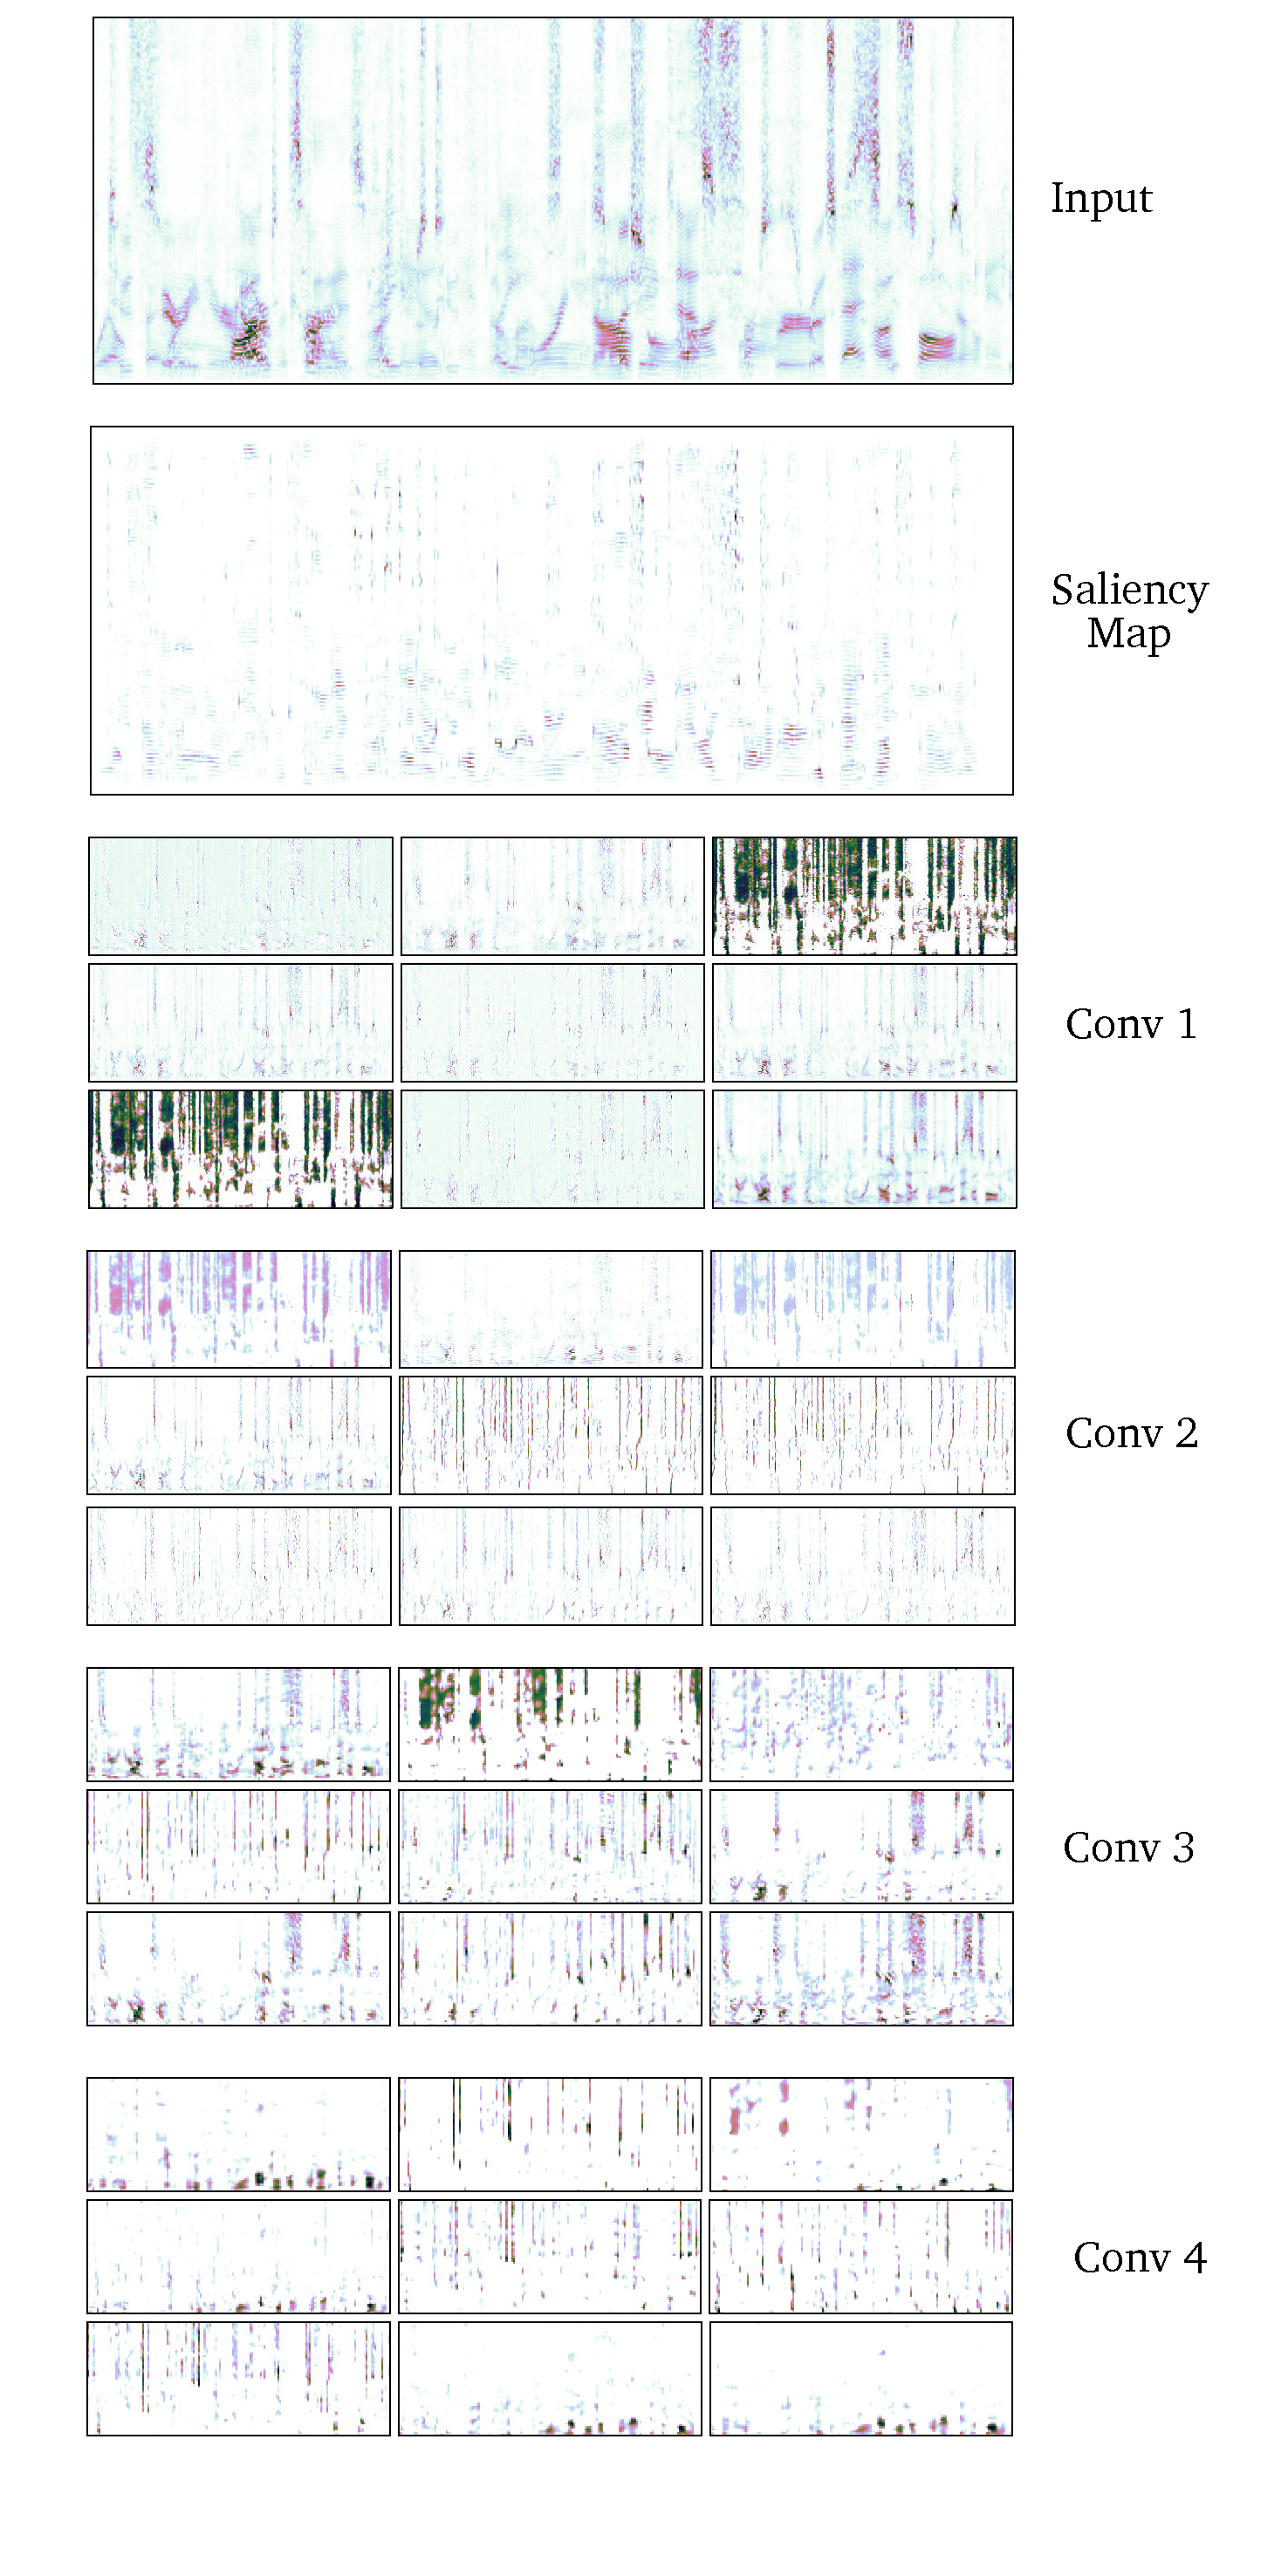
\includegraphics[width=\columnwidth, height=0.7\paperheight, keepaspectratio]{Chapters/08_Analysis_CountNet/figures/outputs.pdf}
  \caption{Illustration of intermediate outputs from the proposed CRNN for each convolutional layer for a given input with \(k=3\) speakers. Saliency map shows positive saliency of guided backpropagation~\cite{Springenberg14}. For each convolutional layer the nine most relevant filters were selected based on their loss with respect to the input. \textsuperscript{\textregistered}2019 IEEE.}%
\label{fig:convoutputs}
\end{figure}
In this section, we focus on the problem of interpreting the strategy undergone by this system for successfully estimating counts.

\subsection{Saliency Maps}
We first conducted a visual analysis based on salience map representations~\cite{simonyan13}.
In the deep learning context, saliency maps are visualizations that are able to show which specific input elements are important given a specific output prediction. In vision, this allows to show which pixels were most relevant to make up the decision to activate a specific output class. 
In the case of audio it can highlight which time-frequency bins in a spectrogram are most relevant.
The common idea is to compute the gradient of the model's prediction with respect to the input, holding the weights fixed. This determines which input elements need to be changed the least to affect the prediction the most.
\par
In this work, we used guided backpropagation, first introduced in~\cite{Springenberg14} and successfully deployed in~\cite{schluter16} to compute a saliency map for singing voice detection.
For a given input of a three-speaker mixture, we depicted the saliency map in Fig.~\ref{fig:convoutputs}.
The saliency map indicates that our proposed model does not rely much on the overlapped parts but instead utilize many of the single speaker time-frequency bins as well as many high-frequency components such as plosives and fricative phonemes.\par
While the saliency map confirms that the network does exploit both low and high-frequency content from the input signal, it is not sufficient to conjecture about the strategy implemented in the network.

\subsection{Ablation Analysis}
To provide further insight, we propose another layer-wise analysis, that provides information concerning the behavior of the model at different successive layers.
While we cannot show all filter outputs (e.g. 64, for the first layer), instead, for each filter, we compute its loss with respect to the input of the model using gradient update and sort the filters according to their loss behavior.\par

Figure~\ref{fig:convoutputs} depicts the nine highest loss outputs per convolutional layer.
We can observe that while the first layer shows only low-level variations of the input, already the second layer seems to be more abstract and emphasizes phoneme segmentations based on mid and high frequency content.
While filter outputs of layer 3 and 4 also show more low-frequency content such as the harmonic signals, the overall visual impression is that the proposed CRNN focuses on the temporal segmentation of phonemes.\par

The conducted analysis suggests that the network is doing count estimation based on the detection of phonemes. To assess the validity of this interpretation, we directly verified the performance of the method as a function of the phoneme activity. In the following, we verify whether count estimates are affected by the pronunciation speed.\par

We assume that the CRNN model learned the aggregated phoneme or syllable activity of all speakers in a fixed, given excerpt.

If that is the case, it would mean that the speaker count estimate would be affected if the speakers would speak slower or faster in relation to the fixed input window (speaking rate).
We therefore want to see if very slow or very fast speakers significantly increase the error of our proposed CRNN model.
In turn we define a null hypothesis that there is no association between the speaker count error probability and the value of the \emph{speaking rate}.\par

To verify our hypothesis, we created another experiment based on the \emph{TIMIT} dataset.
It comes with phoneme and word level annotations, from which the speaking rate (defined as syllables per second) can be computed for each input sample~\cite{Jiao16}.
To reduce the influence of the different acoustical environment in TIMIT compared to Libri Speech, we retrained the CRNN classification model on the \emph{TIMIT} training dataset, using the same parameters as described in Section~\ref{ssec:parameters}.
At test time we randomly generated 5 seconds excerpts of \(k=6\) from the TIMIT test subset and predicted the error \(E(k) = \hat{k} - k\) for each CRNN output.
We grouped the estimates into three classes: \(E(k) = 0\) (correct response), \(E(k) > 0\) (overestimation), \(E(k) < 0\) (underestimation).
For \(k=6\) we ended up with two groups of results because overestimation did not take place.
From the remaining two groups \emph{underestimation} and \emph{correct} responses we randomly selected 1000 samples each, resulting in an total sample size of \(n=2000\).
For these samples we computed an average speaking rate of \(3.40\) syllables per second and a standard deviation of \(0.2\).\par

We chose a Generalized Linear Model (GLM) for the statistical test, as described in~\cite{jaeger08}.
This allows us model the results with a binary logit regression model that turns the mean of E into a binomially distributed probability modeled by log linear values: \(\mbox{logit}(E) \sim \mbox{Intercept} + \beta \cdot{\mbox{Speaking Rate}}\).
\begin{table}[t]
\begin{center}
\begin{tabular}{lcccc}
\toprule
                        & \textbf{coef} & \textbf{std err} & \textbf{z} & \textbf{P$>$$|$z$|$} \\
\midrule
\textbf{speaking rate} &      -1.2697   &        0.232     &     -5.477  &         0.000        \\
\textbf{intercept}          &      4.3213  &        0.790     &    5.468  &         0.000  \\
\bottomrule
\end{tabular}
\caption{Results of a binary logit regression test for the dependent variable \emph{correct response} over the independent variable \emph{speaking rate}. The results are based on $n=2000$ randomly drawn results of the CRNN model trained and evaluated on the TIMIT dataset.}%
\label{tab:logit}
\end{center}
\end{table}
The results of our test are shown in Table~\ref{tab:logit} and indicate the speaking rate has statistically significant influence on the error \(p < 0.05, df=1, \textrm{Pseudo}\ R^2=0.0111\).
To better understand the effect of our predictor, we computed an odds ratio \(\exp(\mbox{speaking rate}) = 0.28\).\par
This indicates that a decrease in speaking rate of 1 syllable per second will increase the likeliness of an underestimation error by 28 percent.
Even though this is considered as a small effect size, it gives an interesting hint for the strategy taken of our proposed model and also suggests that for improved robustness, training would benefit from a large variety of speaking rates.
Furthermore, it still remains unclear if the model would suffer from languages with a speaking rate which is naturally higher or lower than English or Chinese (see~\cite{Osser64}).

\section{Summary and Discussion}%
\label{sec:conclusion}

We introduced the task of estimating the maximum number of concurrent speakers in a simulated ``cocktail-party'' environment using a data-driven approach, discussing how to frame this task in a deep learning context.
Building upon earlier work, we investigated what method is best to output integer source count estimates and also defined suitable cost functions for optimization.
In a comprehensive study, we performed experiments to evaluate different network architectures.
Furthermore, we investigated and evaluated other important parameters such as input representations or the input duration.
Our final proposed model uses a convolutional recurrent (CRNN) architecture, based on classification at the network's output.
Compared to several baselines, our proposed model has a significantly lower error rate;
it achieves error rates of less than 0.3 speakers in mean absolute error for classifying zero to ten speakers---a decrease of 28.95\% compared to~\cite{stoeter17}.
In further simulations, we revealed that our model is robust to unseen languages (such as Chinese), as well as varying acoustical conditions (except for reverberation, where the error increased significantly).
However, including reverberated samples in the training reduces the error.
Additionally, we conducted a perceptual experiment showing that these results clearly outperform humans.
We hope our research stimulates future research on data-driven count estimation, a task that currently lacks real-world datasets.
Future methods could also work on further reducing the duration of excerpts to improve the conceptual latency.\par
Lastly, in an ablation study, we found that the CRNN uses a strategy to segment phonemes/syllables to estimate the count.
Hence, we hypothesize that a speaker count estimate is influenced by the average speaking rates of certain languages.
To underpin this hypothesis, we showed that the speaking rate has a significant effect on the error of our model.
Interestingly, the speaking rate is an important source of modulations in speech~\cite{plomp83} and this discovery establishes a link between speech analysis in humans and machines.



%\addtocontents{toc}{\protect\clearpage} % <--- just debug stuff, ignore
% %************************************************
\chapter{Math Test Chapter}\label{ch:mathtest} % $\mathbb{ZNR}$
%************************************************
Ei choro aeterno antiopam mea, labitur bonorum pri no. His no decore
nemore graecis. In eos meis nominavi, liber soluta vim cu. Sea commune
suavitate interpretaris eu, vix eu libris efficiantur.

\section{Some Formulas}
Due to the statistical nature of ionisation energy loss, large
fluctuations can occur in the amount of energy deposited by a particle
traversing an absorber element\footnote{Examples taken from Walter
Schmidt's great gallery: \\
\url{http://home.vrweb.de/~was/mathfonts.html}}.  Continuous processes
such as multiple
scattering and energy loss play a relevant role in the longitudinal
and lateral development of electromagnetic and hadronic
showers, and in the case of sampling calorimeters the
measured resolution can be significantly affected by such fluctuations
in their active layers.  The description of ionisation fluctuations is
characterised by the significance parameter $\kappa$, which is
proportional to the ratio of mean energy loss to the maximum allowed
energy transfer in a single collision with an atomic electron:
\graffito{You might get unexpected results using math in chapter or
section heads. Consider the \texttt{pdfspacing} option.}
\begin{equation}
\kappa =\frac{\xi}{E_{\textrm{max}}} %\mathbb{ZNR}
\end{equation}
$E_{\textrm{max}}$ is the maximum transferable energy in a single
collision with an atomic electron.
\[
E_{\textrm{max}} =\frac{2 m_{\textrm{e}} \beta^2\gamma^2 }{1 +
2\gamma m_{\textrm{e}}/m_{\textrm{x}} + \left ( m_{\textrm{e}}
/m_{\textrm{x}}\right)^2}\ ,
\]
where $\gamma = E/m_{\textrm{x}}$, $E$ is energy and
$m_{\textrm{x}}$ the mass of the incident particle,
$\beta^2 = 1 - 1/\gamma^2$ and $m_{\textrm{e}}$ is the electron mass.
$\xi$ comes from the Rutherford scattering cross section
and is defined as:
\begin{eqnarray*} \xi  = \frac{2\pi z^2 e^4 N_{\textrm{Av}} Z \rho
\delta x}{m_{\textrm{e}} \beta^2 c^2 A} =  153.4 \frac{z^2}{\beta^2}
\frac{Z}{A}
  \rho \delta x \quad\textrm{keV},
\end{eqnarray*}
where

\begin{tabular}{ll}
$z$          & charge of the incident particle \\
$N_{\textrm{Av}}$     & Avogadro's number \\
$Z$          & atomic number of the material \\
$A$          & atomic weight of the material \\
$\rho$       & density \\
$ \delta x$  & thickness of the material \\
\end{tabular}

$\kappa$ measures the contribution of the collisions with energy
transfer close to $E_{\textrm{max}}$.  For a given absorber, $\kappa$
tends
towards large values if $\delta x$ is large and/or if $\beta$ is
small.  Likewise, $\kappa$ tends towards zero if $\delta x $ is small
and/or if $\beta$ approaches $1$.

The value of $\kappa$ distinguishes two regimes which occur in the
description of ionisation fluctuations:

\begin{enumerate}
\item A large number of collisions involving the loss of all or most
    of the incident particle energy during the traversal of an absorber.

    As the total energy transfer is composed of a multitude of small
    energy losses, we can apply the central limit theorem and describe
    the fluctuations by a Gaussian distribution.  This case is
    applicable to non-relativistic particles and is described by the
    inequality $\kappa > 10 $ (\ie, when the mean energy loss in the
    absorber is greater than the maximum energy transfer in a single
    collision).

\item Particles traversing thin counters and incident electrons under
    any conditions.

    The relevant inequalities and distributions are $ 0.01 < \kappa < 10
    $,
    Vavilov distribution, and $\kappa < 0.01 $, Landau distribution.
\end{enumerate}


\section{Various Mathematical Examples}
If $n > 2$, the identity
\[
    t[u_1,\dots,u_n] = t\bigl[t[u_1,\dots,u_{n_1}], t[u_2,\dots,u_n]
    \bigr]
\]
defines $t[u_1,\dots,u_n]$ recursively, and it can be shown that the
alternative definition
\[
    t[u_1,\dots,u_n] = t\bigl[t[u_1,u_2],\dots,t[u_{n-1},u_n]\bigr]
\]
gives the same result.

%*****************************************
%*****************************************
%*****************************************
%*****************************************
%*****************************************

%\include{multiToC} % <--- just debug stuff, ignore for your documents
% ********************************************************************
% Backmatter
%*******************************************************
\appendix
%\renewcommand{\thechapter}{\alph{chapter}}
\cleardoublepage
\part{Appendix}
% %********************************************************************
% Appendix
%*******************************************************
% If problems with the headers: get headings in appendix etc. right
%\markboth{\spacedlowsmallcaps{Appendix}}{\spacedlowsmallcaps{Appendix}}
\chapter{Appendix Test}
Lorem ipsum at nusquam appellantur his, ut eos erant homero
concludaturque. Albucius appellantur deterruisset id eam, vivendum
partiendo dissentiet ei ius. Vis melius facilisis ea, sea id convenire
referrentur, takimata adolescens ex duo. Ei harum argumentum per. Eam
vidit exerci appetere ad, ut vel zzril intellegam interpretaris.

Errem omnium ea per, pro congue populo ornatus cu, ex qui dicant
nemore melius. No pri diam iriure euismod. Graecis eleifend
appellantur quo id. Id corpora inimicus nam, facer nonummy ne pro,
kasd repudiandae ei mei. Mea menandri mediocrem dissentiet cu, ex
nominati imperdiet nec, sea odio duis vocent ei. Tempor everti
appareat cu ius, ridens audiam an qui, aliquid admodum conceptam ne
qui. Vis ea melius nostrum, mel alienum euripidis eu.

\section{Appendix Section Test}
Ei choro aeterno antiopam mea, labitur bonorum pri no. His no decore
nemore graecis. In eos meis nominavi, liber soluta vim cu. Sea commune
suavitate interpretaris eu, vix eu libris efficiantur.

\autoref{tab:moreexample}

\graffito{More dummy text.}
Nulla fastidii ea ius, exerci suscipit instructior te nam, in ullum
postulant quo. Congue quaestio philosophia his at, sea odio autem
vulputate ex. Cu usu mucius iisque voluptua. Sit maiorum propriae at,
ea cum primis intellegat. Hinc cotidieque reprehendunt eu nec. Autem
timeam deleniti usu id, in nec nibh altera.

\section{Another Appendix Section Test}
Equidem detraxit cu nam, vix eu delenit periculis. Eos ut vero
constituto, no vidit propriae complectitur sea. Diceret nonummy in
has, no qui eligendi recteque consetetur. Mel eu dictas suscipiantur,
et sed placerat oporteat. At ipsum electram mei, ad aeque atomorum
mea.

\begin{table}
    \myfloatalign
  \begin{tabularx}{\textwidth}{Xll} \toprule
    \tableheadline{labitur bonorum pri no} & \tableheadline{que vista}
    & \tableheadline{human} \\ \midrule
    fastidii ea ius & germano &  demonstratea \\
    suscipit instructior & titulo & personas \\
    %postulant quo & westeuropee & sanctificatec \\
    \midrule
    quaestio philosophia & facto & demonstrated \\
    %autem vulputate ex & parola & romanic \\
    %usu mucius iisque & studio & sanctificatef \\
    \bottomrule
  \end{tabularx}
  \caption[Autem usu id]{Autem usu id.}
  \label{tab:moreexample}
\end{table}

Ei solet nemore consectetuer nam. Ad eam porro impetus, te choro omnes
evertitur mel. Molestie conclusionemque vel at, no qui omittam
expetenda efficiendi. Eu quo nobis offendit, verterem scriptorem ne
vix.

  
\begin{lstlisting}[float,caption=A floating example]
for i:=maxint to 0 do
begin
{ do nothing }
end;
\end{lstlisting}
%********************************************************************
% Other Stuff in the Back
%*******************************************************
\cleardoublepage%********************************************************************
% Bibliography
%*******************************************************
% work-around to have small caps also here in the headline
% https://tex.stackexchange.com/questions/188126/wrong-header-in-bibliography-classicthesis
% Thanks to Enrico Gregorio
\defbibheading{bibintoc}[\bibname]{%
  \phantomsection
  \manualmark
  \markboth{\spacedlowsmallcaps{#1}}{\spacedlowsmallcaps{#1}}%
  \addtocontents{toc}{\protect\vspace{\beforebibskip}}%
  \addcontentsline{toc}{chapter}{\tocEntry{#1}}%
  \chapter*{#1}%
}
\printbibliography[heading=bibintoc]

% Old version, will be removed later
% work-around to have small caps also here in the headline
%\manualmark
%\markboth{\spacedlowsmallcaps{\bibname}}{\spacedlowsmallcaps{\bibname}} % work-around to have small caps also
%\phantomsection
%\refstepcounter{dummy}
%\addtocontents{toc}{\protect\vspace{\beforebibskip}} % to have the bib a bit from the rest in the toc
%\addcontentsline{toc}{chapter}{\tocEntry{\bibname}}
%\label{app:bibliography}
%\printbibliography

\cleardoublepage%*******************************************************
% Declaration
%*******************************************************
\refstepcounter{dummy}
\pdfbookmark[0]{Declaration}{declaration}
\chapter*{Declaration}
\thispagestyle{empty}
Put your declaration here.
\bigskip

\noindent\textit{\myLocation, \myTime}

\smallskip

\begin{flushright}
    \begin{tabular}{m{5cm}}
        \\ \hline
        \centering\myName \\
    \end{tabular}
\end{flushright}

\cleardoublepage\pagestyle{empty}

\hfill

\vfill


\pdfbookmark[0]{Colophon}{colophon}
\section*{Colophon}
This document was typeset using the typographical look-and-feel \texttt{classicthesis} developed by Andr\'e Miede. 
The style was inspired by Robert Bringhurst's seminal book on typography ``\emph{The Elements of Typographic Style}''. 
\texttt{classicthesis} is available for both \LaTeX\ and \mLyX: 
\begin{center}
\url{https://bitbucket.org/amiede/classicthesis/}
\end{center}
Happy users of \texttt{classicthesis} usually send a real postcard to the author, a collection of postcards received so far is featured here: 
\begin{center}
\url{http://postcards.miede.de/}
\end{center}
 
\bigskip

\noindent\finalVersionString

%Hermann Zapf's \emph{Palatino} and \emph{Euler} type faces (Type~1 PostScript fonts \emph{URW
%Palladio L} and \emph{FPL}) are used. The ``typewriter'' text is typeset in \emph{Bera Mono}, 
%originally developed by Bitstream, Inc. as ``Bitstream Vera''. (Type~1 PostScript fonts were made 
%available by Malte Rosenau and
%Ulrich Dirr.)

%\paragraph{note:} The custom size of the textblock was calculated
%using the directions given by Mr. Bringhurst (pages 26--29 and
%175/176). 10~pt Palatino needs  133.21~pt for the string
%``abcdefghijklmnopqrstuvwxyz''. This yields a good line length between
%24--26~pc (288--312~pt). Using a ``\emph{double square textblock}''
%with a 1:2 ratio this results in a textblock of 312:624~pt (which
%includes the headline in this design). A good alternative would be the
%``\emph{golden section textblock}'' with a ratio of 1:1.62, here
%312:505.44~pt. For comparison, \texttt{DIV9} of the \texttt{typearea}
%package results in a line length of 389~pt (32.4~pc), which is by far
%too long. However, this information will only be of interest for
%hardcore pseudo-typographers like me.%
%
%To make your own calculations, use the following commands and look up
%the corresponding lengths in the book:
%\begin{verbatim}
%    \settowidth{\abcd}{abcdefghijklmnopqrstuvwxyz}
%    \the\abcd\ % prints the value of the length
%\end{verbatim}
%Please see the file \texttt{classicthesis.sty} for some precalculated 
%values for Palatino and Minion.
%
%    \settowidth{\abcd}{abcdefghijklmnopqrstuvwxyz}
%    \the\abcd\ % prints the value of the length





% ********************************************************************
% Game Over: Restore, Restart, or Quit?
%*******************************************************
\end{document}
% ********************************************************************
